\documentclass[tcc]{ic}

\usepackage{indentfirst}
\usetikzlibrary{decorations}
\usetikzlibrary{shapes.symbols}
\usetikzlibrary{shapes.arrows}
\usepackage{icomma}
\usepackage{microtype}
\usepackage[binary-units]{siunitx}
\usepackage{pdfpages}

\newenvironment{demonst} 
               {\noindent \textit{\textbf{Demonstração.}}~ }	% begin demonst
               {\hfill\rule{2mm}{2mm} \vspace{\parskip} } 	% end demonst

\newtheorem{definicao}{Definição}[section]
\newtheorem{teorema}{Teorema}[section]
\newtheorem{lema}{Lema}
\newtheorem{corolario}{Corolário}
\newtheorem{proposicao}{Proposição}

\graphicspath{{../newPlots/}}

%======================================================%
%=========== Informações do documento PDF =============%
%======================================================%
\hypersetup{
colorlinks = {true},
linktocpage = {false},
plainpages = {false},
linkcolor = {Blue},
citecolor = {Blue},
urlcolor = {Red},
unicode = {true},
pdftitle ={Teste para Verificação da Hipótese de Ruído Branco utilizando Teoria da Informação},
pdfauthor = {Marcelo Queiroz de Assis Oliveira},
pdfsubject = {Disserta\c c\~ao de Mestrado},
pdfkeywords={Geradores de Números Aleatórios. Testes Teóricos. Testes Estatísticos. Teoria da Informação.},
pdfcreator = {LaTeX2e},
pdffitwindow = {false},
pdfstartview = {FitH},
pdftoolbar = {true},
pdfpagemode = {UseOutlines},
pdfview = {XYZ null null null}
}

%======================================================%
%================ CAPA DA DISSERTAÇÃO =================%
%======================================================%

\titulo{Teste para Verificação da Hipótese de Ruído Branco utilizando Teoria da Informação}

\autor{Marcelo Queiroz de Assis Oliveira}{marceloqao@gmail.com}{http://sites.google.com/site/marceloqao/}

\orientador{Dr. Alejandro C.\ Frery}{http://sites.google.com/site/acfrery/}{Instituto de Computação}{Universidade Federal de Alagoas}

\orientadorDois{Dr. Heitor Soares Ramos Filho}{https://sites.google.com/a/ic.ufal.br/heitor/}{Instituto de Computação}{Universidade Federal de Alagoas}

\examinador{Dr. Osvaldo Anibal Rosso}{oarosso@gmail.com}{Instituto de Física}{Universidade Federal de Alagoas}

\examinadorDois{Dra.\ Juliana Gambini}{mgambini@itba.edu.ar}{Departamento de Ingeniería Informática}{Instituto Tecnológico de Buenos Aires}

% \examinadorQuatro{Examinador 4}{ex4@email.com}{Instituto ou Departamento}{Universidade do Examinador 4}

\dataMesAno{Novembro}{2017}

\begin{document}

\selectlanguage{portuguese}

\capa

% %======================================================%
% %================= Aprovação - Banca ==================%
% %======================================================%
\newpage
\thispagestyle{empty}
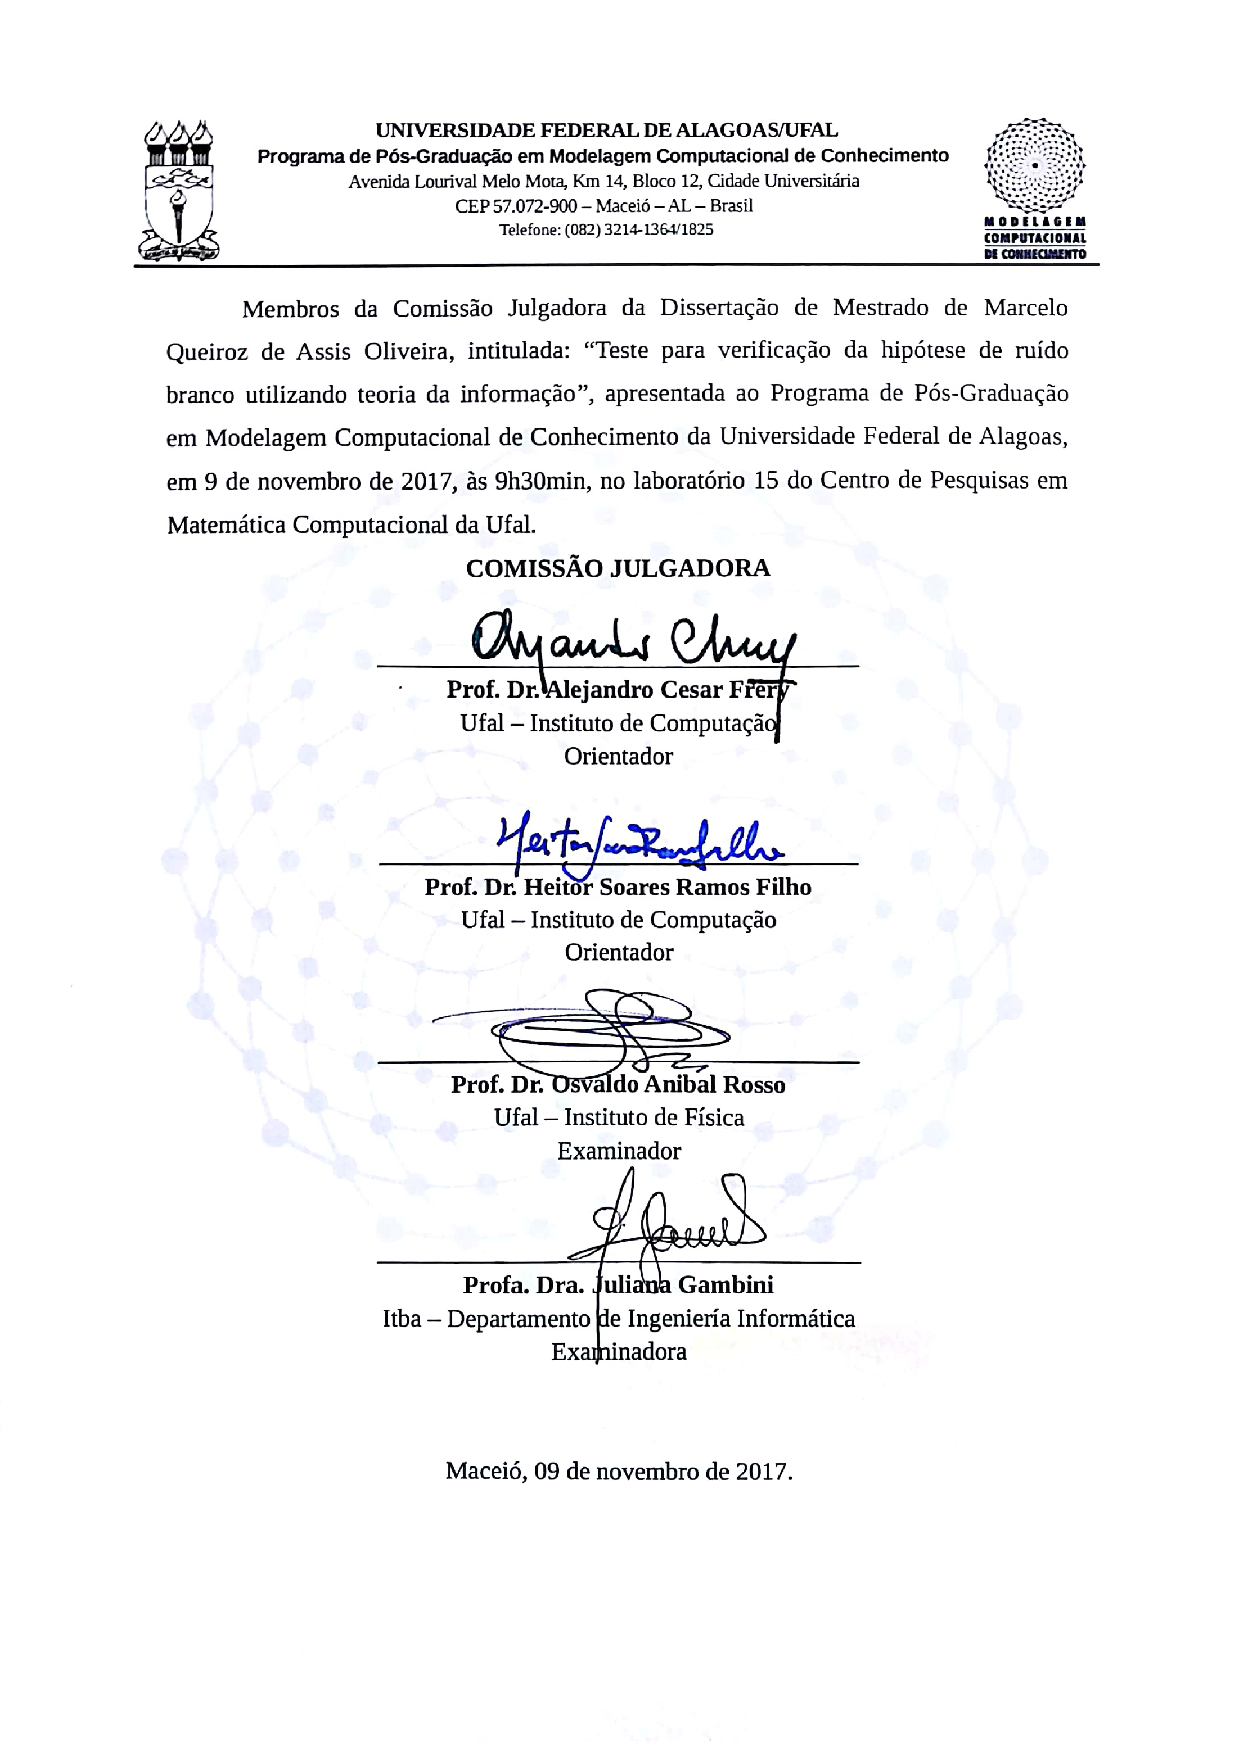
\includepdf[pages=1]{assinaturas_banca.pdf}

% %======================================================%
% %====================== DEDICAÇÃO =====================%
% %======================================================%
 \newpage
 \thispagestyle{empty}
 \mbox{}\vfill
 \begin{flushright}
 À minha amada esposa Élida, aos meus \emph{filhos} Duda, \\
 Gabriel, João Marcelo e Melissa, a minha querida Mãe,\\
 Francisca \textit{(In Memorian)} dedico este trabalho. \\
 Por vocês, faria tudo de novo.
 \end{flushright}

%======================================================%
%======================= RESUMO =======================%
%======================================================%
\begin{resumo}
\noindent 
O nosso ponto de partida é o desejo de analisar
se é viável verificar no plano ($H\times C$), dentro de uma abordagem estatística, se sequências de observações são ruído branco.

Na literatura encontramos diversos trabalhos que fazem isso de forma ``ad hoc'', verificando se o ponto característico de uma sequência nesse plano é próximo ao ponto ($1,0$). 
Contudo, tal como afirma \citet{NewPermutationEntropy}, não encontramos análises detalhadas que permitam atribuir significância estatística a tais afirmações.

Para elucidar essa questão, e diante da impossibilidade de contar com sequências infinitamente longas e que garantidamente sejam ruído branco, coletamos sequências de três fontes diferentes: duas físicas e uma algorítmica considerada de qualidade.
Verificamos se é possível considerá-las ideais para os nossos fins.

Analisamos a dispersão dos pontos característicos dessas sequências no plano ($H\times C$) utilizando quatro fatores: o tamanho da sequência ($N$), o tamanho da palavra ($D$), o \textit{delay} $(\tau)$ e a fonte geradora, observando a distância dos pontos característicos ao ponto de referência. Sugiram então evidências de que a fonte geradora seria um fator irrelevante para a análise.

Com o intuito de consolidar essa possibilidade, aplicamos o teste de Kolmogorov-Smirnov a pares de sequências comparáveis, porém verificamos que apenas duas das fontes geradoras são realmente irrelevantes, as duas fontes físicas.

Agrupamos, então os dados das fontes físicas e passamos a tratá-los como nossa referência, em seguida procuramos por regiões de confiança. 
Adotamos uma abordagem não-paramétrica por não termos nenhuma evidência teórica acerca da distribuição que segue a distância do ponto característico ao de referência quando é analisada uma sequência finita de ruído branco.

Calculamos então os quantis, respeitados os fatores tamanho da sequência ($N$), tamanho da palavra ($D$) e \textit{delay} ($\tau$), que servem como regiões de confiança para o teste que deu origem a este trabalho.

Concluímos a dissertação verificando que sequências produzidas por geradores aceitos pela comunidade geram pontos característicos dentro de regiões de confiança, enquanto que um gerador que foi descartado pelas estruturas que as suas sequências apresentam leva a pontos fora dessas mesmas regiões.
Analisamos também sequências estacionárias e não estacionárias, e para as primeiras fazemos uma análise preliminar do poder do teste.

\vspace{1em}
\noindent {\bf Palavras-chave}: Geradores de Números Aleatórios. Testes Teóricos. Testes Estatísticos. Teoria da Informação.
\end{resumo}

%======================================================%
%====================== ABSTRACT ======================%
%======================================================%
\selectlanguage{english}
\begin{abstract}
\noindent
%Our starting point is the desire to verify in the plane ($H\times C$) in a  statistical approach, if sequences of observations are white noise .

We want to verify  if sequences of observations are white noise  in the plane ($H\times C$).

In the literature, we find several works that do this in an ``ad hoc'' way, checking if the characteristic point of a sequence in that plane is close to the point ($1,0$).

However, as \citet{NewPermutationEntropy} states, we do not found detailed analyzes to assign statistical significance to such statements.

To elucidate this question, and in the face of the impossibility of counting infinitely long sequences that are guaranteed to be white noise, we gather candidate sequences from three different sources: two physical and one algorithmic considered as a good source. We checked, if we may consider them ideals for our purposes.

We analyze the dispersion of the characteristic points of these sequences in the plane ($H\times C$) using four factors: the size of the sequence ($N$), the size of the word ($D$), the delay ($\tau$) and the generating source, observing the distance from the characteristic points to the reference point. We observe that the generating source would be an irrelevant factor to the analyses.

To verify this hipothesis, we applied the Kolmogorov-Smirnov test to pairs of comparable sequences, however we verify that only two sources are equivalents, the both physical.

Therefore, we grouped the data from physical sources, and it became our groundtruth, then in sequence, we searched for trust regions. We adopted a non-parametric approach because we did not have no theoretical evidence about the distribution that follows the distance from the characteristic point to our groundtruth when a finite sequence of white noise candidate is analyzed.

We then calculated the quantiles, respecting the factors sequence size ($N$), size of the word ($D$) and delay ($\tau$), which serve as confidence regions for the test that gave rise to this work.

We conclude the dissertation by verifying that sequences produced by community accepted generators generate characteristic points within confidence regions, while a generator that has been discarded by the structures that its sequences present leads to points outside these regions.
We also applied the test to stationary and nonstationary sequences and, for the former, we make a preliminary assessment of the test power.

\vspace{1em}
\noindent 
{\bf Keywords}: Random Number Generators. Theoretical tests. Statistical Tests. Information theory.
\end{abstract}

%======================================================%
%=================== AGRADECIMENTOS ===================%
%======================================================%
\selectlanguage{portuguese}
\begin{agradecimentos}
\noindent

A Deus pelo dom da vida e por manter-me são durante o desenvolvimento deste trabalho.

A meus Pais pelos ensinamentos que não temos dentro da escola e pelo incentivo a buscar o aperfeiçoamento intelectual.

A minha esposa Elida, pelo companheirismo em tudo!

A meus filhos, Maria Eduarda, Gabriel, João Marcelo e Melissa, por sua enorme alegria de viver e seu sorriso.

Aos colegas do mestrado, com os quais vivi frutíferos e divertidos momentos de estudo, valeu Rodrigo, Domarques, Davy, 
Felipe, Brião, Pedro, Torres e todos os colegas do curso e do LaCCAN.

Ao colega Joao Borges pela grande contribuição na implementação.

Ao Professor Christoph Marquardt do \textit{Max Planck Institute for the Science of Light} e ao Professor Mads Haahr do \textit{Trinity College Dublin} e criador do \textit{www.random.org} pela gentileza em fornecer dados realmente aleatórios, sem os quais este trabalho não teria sido realizado.

A todos os colegas da UFAL que direta ou indiretamente contribuiram para este trabalho, no LCCV, NTI e na gesão central da universidade, em especial ao companheiro Kleymerson por segurar a barra durante os momentos finais e também à Magnífica Reitora da UFAL, Valéria Correia e José Vieira, Vice Reitor. E ainda a todos que sempre inquiriam acerca do desenvolvimento deste trabalho.

Aos servidores do Instito de Computação da UFAL, em especial Vitor Torres pela presteza e atenção em atender os alunos do curso de Mestrado em Modelagem Computacional de Conhecimento, da mesma forma aos professores do curso.

Ao professor Osvaldo Rosso pela imensa contribuição relativa à teoria da informação e pelas ricas conversas acerca do tema

E finalmente aos meus orientadores, Alejandro Frery e Heitor Ramos sem os quais este trabalho não teria se concretizado, obrigado pelo incentivo, pela disponibilidade e pela paciência. 

Muito obrigado!!

\vspace{1em}
\begin{flushright}
Marcelo Queiroz de A. Oliveira
\end{flushright}
\end{agradecimentos}

%======================================================%
%====================== EPÍGRAFE ======================%
%======================================================%
% \newpage
% \thispagestyle{empty}
% \mbox{}\vfill
% \begin{flushright}
% \emph{``frase.''}\\
% \vspace{1em}
% \textbf{Autor}
% \end{flushright}

%======================================================%
%======================= LISTAS =======================%
%======================================================%
\mylistoffigure

\mylistoftable

% \mylistofalgorithm

%\mylistofequation

\mylistofcontents

\inicio
\setcounter{page}{9} %verificar quantas páginas possuem até iniciar o capítulo 1 (subtraindo capa, folha de aprovação e catalogação).


%\mychapter{Introdução}{chp:introducao}
\lhead{INTRODUÇÃO}

  \lettrine{}{} 

\section{Motivação}
  
%   \lettrine{N}{a} .


\section{Visão geral}



%\section{Contribuições}

%   O trabalho proposto visa contribuir no tocante à sobrevida de Redes de Sensores sem Fios, aumentando o tempo de funcionamento das mesmas através da maior disponibilidade de energia nos nós que a constituem. O trabalho se apoia na estabilidade, desempenho e confiabilidade da linguagem R \citep{R} fazendo uso das boas práticas de \emph{Reproducible Research} como apresentadas em \citet{RR2010}.


%\section{Riscos}

%   Há riscos envolvidos no processo Científico aqui tratado, dentre eles, pode-se citar

\begin{center}
	\fbox{
	\colorbox[RGB]{227, 227, 227}{
	\parbox[t]{.8\linewidth}
		{Neste capítulo foram tratados os aspectos introdutórios ao tema como a motivação e uma visão geral do mesmo, no próximo capítulo é feita uma fundamentaćão teórica visando fundamentar a idéias propostas no trabalho.}} }
\end{center}

\mychapter{Introdução e Delimitação do Problema}{chp:Fundamentação Teórica}
\lhead{Introdução e Delimitação}

% Breve resumo do capítulo.
\lettrine{E}{ste} capítulo tem como objetivo apresentar uma fundamentação teórica necessária para embasar os conceitos aplicados no trabalho.
Delimitaremos aqui o problema a ser tratado nesta tese.

Em relação a fundamentação teórica, utilizou-se como principal fonte de pesquisa a área de indexação de periódicos científicos ISI \emph{Web of Knowledge}, onde foram obtidas a grande maioria das referências, usando como parâmetros o fator de impacto dos periódicos pesquisados, a quantidade de citações de cada publicação, o grau de relevância para o tema pesquisado e o nível de produtividade (fator-H) dos autores envolvidos. 
O apoio em livros, \textit{surveys}, \textit{lecture notes} e ferramentas complementares de busca, como o \emph{Google Acadêmico} foram utilizadas para complementar esta pesquisa.

\section{Números Aleatórios} %Simulação física, Von Neumann, Congruenciais Lineares, etc

A noção de aleatoriedade é fundamental em diversas áreas, entretanto uma definição precisa, até mesmo do ponto de vista matemático rigoroso, é bastante difícil. 
Algumas questões emergem naturalmente como, o que vem a ser aleatoriedade? 
Existem eventos aleatórios na natureza? 
Faz algum sentido buscar leis da aleatoriedade? 
É possível simular a aleatoriedade? 
Estas são questões muito difíceis, envolvendo, inclusive, os primórdios da investigação filosófica como discute \citep{Volchan:02}.
Essa dificuldade é bem ilustrada de forma humorística na Figura~\ref{fig:Dilbert}.

\begin{figure}[hbt]
\centering
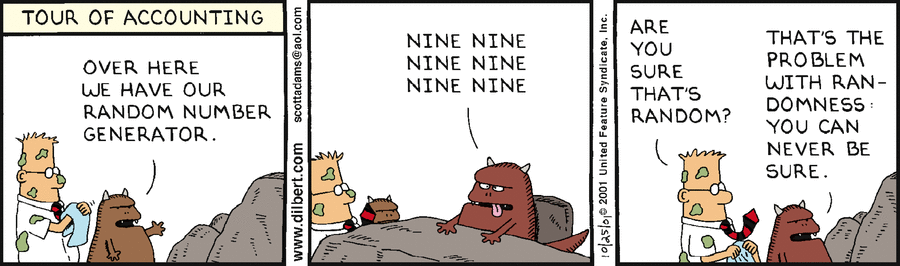
\includegraphics[width=.7\linewidth]{dilbert}
\caption{Visão de Dilbert de um gerador de números aleatórios}\label{fig:Dilbert}
\end{figure}

Números aleatórios perfazem uma das partes mais importantes em aplicações computacionais nos vários campos do conhecimento, como aborda \citep{Knuth:98}:
\begin{itemize}
     \item \textit{Simulação} - Quando um computador é usado para simular fenômenos naturais, números aleatórios são necessários para fazer as coisas de forma realística. Simulação abrange diversas áreas, desde o estudo de física nuclear (onde particulas são submetidas a colisões aleatórias) até pesquisa operacional (como, por exemplo, a taxa de pessoas que entram num aeroporto em intervalos aleatórios).
     \item \textit{Amostragem} - É praticamente impossível examinar todos os possíveis casos, porém uma amostra aleatória provê um palpite sobre como é o comportamento típico do fenômeno em questão.
     \item \textit{Análise Numérica} - Técnicas elaboradas para a solução de complexos problemas numéricos foram desenvolvidas utilizando-se números aleatórios.
     \item \textit{Programação de Computadores} - Valores aleatórios são uma ótima fonte de dados para testar a eficácia de algoritimos computacionais.
     \item \textit{Tomada de Decisão} - Existem relatos de que diversos executivos tomam suas decisões lançando moedas ou atirando dardos. Também há rumores de que professores universitários lançam suas notas de forma similar. Em alguns momentos é importante tomar decisões de forma não influenciada por qualquer agente externo.
     \item \textit{Criptografia} - Uma fonte de bits não viesada é essencial para diversos tipos de comunicações seguras, quando os dados precisam ser mantidos em sigilo.
     \item \textit{Estética} - Um pouco de aleatoriedade faz com que gráficos e músicas geradas por computador aparentem ser menos artificiais.
     \item \textit{Diversão} - Rolar dados, embaralhar cartas, girar rodas de roletas, etc., são passatempos facinantes para muitos. Estes usos tradicionais de números aleatórios sugeriram o nome ``Método de Monte Carlo''.
    \end{itemize}

Existem dois tipos básicos de geradores utilizados para produzir sequências aleatórias: GNAs -- Geradores de Números Aleatórios, do inglês (\textit{RNGs} -- \textit{Random Number Generators}) e GNPA -- Geradores de Números Pseudoaleatórios, do inglês (\textit{PRNGs} -- Pseudorandom Number Generators).

\subsection{Geradores de Números Aleatórios -- GNA}
  
Geradores de Números Aleatórios utilizam uma fonte não determinística juntamente com algumas funções de processamento para produzir aleatoriedade. 
As saídas deste tipo de gerador podem ser usadas diretamente como números aleatórios, desde que satisfaçam critérios de aleatoriedade, ou ainda podem servir como parâmetro de entrada para geradores de números pseudoaleatórios, vistos com mais detalhes na sequência. 

A maior parte dos geradores utiliza-se de fenômenos físicos naturais como, decaimento radioativo, ruidos termais em semiconcutores, amostras de som num local ruidoso, ruído no espectro eletromagnético, dentre outros que, por óbvia dedução, carecem de algum hardware específico para serem capturados. 

Na literatura é possível encontrar trabalhos relatando detalhadamente a criação de geradores de números aleatórios utilizando fontes de aleatoriedade apropriadas.
\citet{Fairfield:85} descrevem a geração de um fluxo de bits aleatórios baseado na instabilidade da frequência de um oscilador.
Evidentemente a construção de um gerador como o descrito anteriormente demanda o emprego de técnicas apuradas e um grande conhecimento teórico, além de necessitar, em sua grande maioria, de hardware especializado, o que gera uma barreira para os usuários que demandam tais dados aleatórios.
Desta sorte, frequentemente os usuários precisam se valer de técnicas alternativas para obter aleatoriedade.

\subsection{Geradores de Números Pseudoaleatórios -- GNPA}

Dadas as dificuldades descritas anteriormente, atualmente a maneira mais conveniente e confiável de se gerar números aleatórios para diversas aplicações é através de algoritmos com um sólido embasamento matemático. 
Tais algoritmos produzem sequências de números sabidamente não aleatórios ao todo, mas que aparentam comportar-se como números aleatórios independentes, isto é, tomada uma sequência de variáveis aleatórias independentes e identicamente distribuídas sobre o Intervalo $(0,1)$. 
Tal sequência pode ser chamada de ``Pseudoaleatória'' e o programa utilizado em sua produção de ``Gerador de Números Pseudoaleatórios'' como definem \citet{LEcuyer:98}.

\section{Principais Testes Clássicos} %Revisão Cronológica/Conceitual

Existem duas abordagens para testar-se a capacidade de geradores aleatórios ou pseudoaleatórios produzirem sequências ditas aleatórias.
Segundo \citet{LEcuyer:92} são elencados em teóricos e empíricos.

Os testes teóricos são bastante específicos para cada tipo de GNPA, pois analisam o as propriedades das sequências a partir da definição do gerador.
Já os testes empíricos valem-se de técnicas estatísticas objetivando avaliar o quão boas são as sequências produzidas por um determinado gerador.
Estes últimos podem ser aplicados tanto a GNAs quanto a GNPAs.

Neste trabalho propomos um teste empírico não paramétrico baseado em ferramentas da teoria da informação.
Na seção a seguir daremos uma breve introdução cronológica aos testes disponíveis na literatura e ao estado da arte.
  
% \subsection{Diehard}
 
 \subsection{NIST}
 
Fundado em 1991, o NIST (\textit{National Institute of Standards and Technology}) é uma agência não regulatória do Departamento de Comércio dos Estados Unidos da América que tem por missão promover a inovação e a competitividade nos EUA através da ciência de medidas, padrões e tecnologia de forma a alavancar a segurança econômica e melhorar a qualidade de vida do povo americano.

A sua Divisão de Segurança de Computadores (CSD) e o Centro de Pesquisa em Segurança Computacional (CSRC) facilitam a ampla disseminação de práticas e ferramentas de segurança da informação, provendo recursos para a definição de padrões além de identificar recursos de segurança na Web para suportar usuários na industria, governo e academia. 

CSRC é o portal de acesso primário para se ter acesso às publicações de segurança de computadores, padrões e instruções, além de outras informações relacionadas a segurança.

Desde 1997, o Grupo de Trabalho Técnico em Geração de Números Aleatórios (RNG-TWG) tem trabalhado no desenvolvimento de uma bateria de testes estatísticos apropriados para a avaliação de geradores de números aleatórios e pseudoaleatórios utilizados em aplicações criptográficas. 

Os principais objetivos do grupo são:
  \begin{itemize}
   \item Desenvolvimento de uma bateria de testes estatísticos para detectar não aleatoriedade em sequencias binárias construidas através de geradores de números aleatórios e pseudoaleatórios utilizados em aplicações criptográficas;
   \item Produzir documentação e uma implementação em software destes testes;
   \item Prover auxílio no uso e aplicação destes testes.
  \end{itemize}

%Um total de quinze testes estatísticos foram desenvolvidos, implementados e avaliados. A seguir fazemos um breve descritivo acerca dos testes.

%  \begin{itemize}
%   \item \textbf{Frequency (Monobits) Test} - O foco do teste está na proporção de $zeros$ e $uns$ em toda a sequência. O propósito deste teste é determinar em que momento o número de $zeros$ e $uns$ numa sequência é aproximadamente o mesmo como é o esperado para uma sequência realmente aleatória. O teste avalia a proximidade da porção de $uns$ a $½$, ou seja, o número de $zeros$ e $uns$ numa sequência deve ser o mesmo.
%%    The focus of the test is the proportion of zeroes and ones for the entire sequence. The purpose of this test is to determine whether that number of ones and zeros in a sequence are approximately the same as would be expected for a truly random sequence. The test assesses the closeness of the fraction of ones to ½, that is, the number of ones and zeroes in a sequence should be about the same.
%   \item \textbf{Test For Frequency Within A Block} - O teste avalia a proporção de $zeros$ e $uns$ em blocos de M bits. O propósito principal deste teste é determinar se a frequência de $uns$ em um bloco de $M$ bits é aproximadamente $M/2$.
%%    The focus of the test is the proportion of zeroes and ones within M-bit blocks. The purpose of this test is to determine whether the frequency of ones is an M-bit block is approximately M/2.
%   \item \textbf{Runs Test} -  Dada uma sequência ininterrupta de zeros ou de $uns$, chamaremos esta sequência de ``rodada'' e de ``k'' tamanho da sequência. O objetivo do teste é determinar a proporção de rodadas de zeros e $uns$ de diversos tamanhos ``k'' necessária para caracterizar uma sequência com aleatória. Em particular, este teste determina quando a oscilação enter estas substrings é muito rápida ou muito lenta.
%%    The focus of this test is the total number of zero and one runs in the entire sequence, where a run is an uninterrupted sequence of identical bits. A run of length k means that a run consists of exactly k identical bits and is bounded before and after with a bit of the opposite value. The purpose of the runs test is to determine whether the number of runs of ones and zeros of various lengths is as expected for a random sequence. In particular, this test determines whether the oscillation between such substrings is too fast or too slow.
%   \item \textbf{Test For The Longest Run Of Ones In A Block} - O teste tem como objetivo determinar quando o comprimento da maior rodada de $uns$ na sequência testada é equivalente ao tamanho da maior rodada esperada em uma sequência aleatória. Note que uma irregularidade no tamanho esperado no valor da maior rodada de $uns$ implica que também há uma irregularidade no tamanho esperado da rodada de $zeros$ mais longa.
%%    The focus of the test is the longest run of ones within M-bit blocks. The purpose of this test is to determine whether the length of the longest run of ones within the tested sequence is consistent with the length of the longest run of ones that would be expected in a random sequence. Note that an irregularity in the expected length of the longest run of ones implies that there is also an irregularity in the expected length of the longest run of zeroes. Long runs of zeroes were not evaluated separately due to a concern about statistical independence among the tests.
%   \item \textbf{Random Binary Matrix Rank Test} - O teste avalia a categoria das submatrizes disjuntas da sequência toda. O objetivo do teste é verificar a ocorrência de dependência linear entre substrings de tamanho fixo da sequência original.
%%    The focus of the test is the rank of disjoint sub-matrices of the entire sequence. The purpose of this test is to check for linear dependence among fixed length substrings of the original sequence.
%   \item \textbf{Discrete Fourier Transform (Spectral) Test} - O teste foca nos picos da \texttt{Transformada Rápida de Fourrier} com o propósito de detectar característica periódicas.
%%    The focus of this test is the peak heights in the discrete Fast Fourier Transform. The purpose of this test is to detect periodic features (i.e., repetitive patterns that are near each other) in the tested sequence that would indicate a deviation from the assumption of randomness.
%   \item \textbf{Non-Overlapping (Aperiodic) Template Matching Test} - O teste observa o número de ocorrências de substrings predefinidas com o propósito de rejeitar sequências que possuam muitas ocorrências de um dado padrão aperiódico. Para tal uma janela de $m$ bits é usada para procurar por um padrão específico de "m" bits.
%%    The focus of this test is the number of occurrences of pre-defined target substrings. The purpose of this test is to reject sequences that exhibit too many occurrences of a given non-periodic (aperiodic) pattern. For this test and for the Overlapping Template Matching test, an m-bit window is used to search for a specific m-bit pattern. If the pattern is not found, the window slides one bit position. For this test, when the pattern is found, the window is reset to the bit after the found pattern, and the search resumes.
%   \item \textbf{Overlapping (Periodic) Template Matching Test} - O teste, assim com o o anterior, procura por substrings predefinidas de rodadas de $uns$ com um dado tamanho. O objetivo do teste é rejeitar sequências que mostrem um desvio do número esperado de $uns$ de um dado tamanho. Note que, quando há um desvio no número de $uns$, este desvio também ocorre com o número de $zeros$. Da mesma forma que o teste anterior, uma janela de $m$ bits é usada para detectar a presença de padrões.
%%    The focus of this test is the number of pre-defined target substrings. The purpose of this test is to reject sequences that show deviations from the expected number of runs of ones of a given length. Note that when there is a deviation from the expected number of ones of a given length, there is also a deviation in the runs of zeroes. Runs of zeroes were not evaluated separately due to a concern about statistical independence among the tests. For this test and for the Non-overlapping Template Matching test, an m-bit window is used to search for a specific m-bit pattern. If the pattern is not found, the window slides one bit position. For this test, when the pattern is found, the window again slides one bit, and the search is resumed.
%   \item \textbf{Maurer's Universal Statistical Test} - O teste observa o número de bits entre padrões casados com o objetivo de detectar ou não se a sequência pode ser significativamente comprimida sem a perda de informação. Uma sequência que pode ser totalmente comprimida é considerada como não aleatória.
%%    The focus of this test is the number of bits between matching patterns. The purpose of the test is to detect whether or not the sequence can be significantly compressed without loss of information. An overly compressible sequence is considered to be non-random.
%   \item \textbf{Linear Complexity Test} - O teste focaliza no tamanho de um registro gerador de informação com o objetivo de determinar quando ou não a sequência é complexa o suficiente para ser considerada aleatória. Sequências aleatórias são caracterizadas por um registro gerador de informação longo.
%%    The focus of this test is the length of a generating feedback register. The purpose of this test is to determine whether or not the sequence is complex enough to be considered random. Random sequences are characterized by a longer feedback register. A short feedback register implies non-randomness.
%   \item \textbf{Serial Test} - O teste detem o foco sobre a frequência de cada bit e de todos os padrões sobrepostos de $m$ bits em toda a sequência, com o propósito de determinar quando o número de ocorrências de padrões sobrepostos de 2m $m$ bits é o mesmo do esperado para sequências aleatórias, sabendo que o padrão pode ser sobreposto.
%%    The focus of this test is the frequency of each and every overlapping m-bit pattern across the entire sequence. The purpose of this test is to determine whether the number of occurrences of the 2m m-bit overlapping patterns is approximately the same as would be expected for a random sequence. The pattern can overlap.
%   \item \textbf{Approximate Entropy Test} - O teste se detém na frequência de cada um dos padrões sobrepostos de $m$ bits com o objetivo de comparar a frequência de dois blocos sobrepostos de tamanhos consecutivos/adjacentes ($m$ e $m+1$) com os valores esperados para uma sequência aleatória.
%%    The focus of this test is the frequency of each and every overlapping m-bit pattern. The purpose of the test is to compare the frequency of overlapping blocks of two consecutive/adjacent lengths (m and m+1) against the expected result for a random sequence.
%   \item \textbf{Cumulative Sum (Cusum) Test} - O teste verifica a distância máxima do ``passeio aleatório'' definido pela soma dos dígitos ajustados ($-1$, $+1$) na sequência com o objetivo de determinar quando a soma cumulativa da sequência parcial que ocorre nas sequências testadas é muito grande ou muito pequeno em relação ao comportamento esperado para sequências aleatórias. Esta sequência cumulativa pode ser considerada como um ``passeio aleatório''. Para uma sequência aleatória, o ``passeio aleatório'' deve ser próximo a $zero$ e para sequências não aleatórias a excursão máxima do ``passeio aleatório'' se distancia de zero e tende a ser grande.
%%    The focus of this test is the maximal excursion (from zero) of the random walk defined by the cumulative sum of adjusted (-1, +1) digits in the sequence. The purpose of the test is to determine whether the cumulative sum of the partial sequences occurring in the tested sequence is too large or too small relative to the expected behavior of that cumulative sum for random sequences. This cumulative sum may be considered as a random walk. For a random sequence, the random walk should be near zero. For non-random sequences, the excursions of this random walk away from zero will be too large.
%   \item \textbf{Random Excursions Test} - O teste verifica o número de ciclos que possuem exatamente $K$ visitas em uma soma cumulativa do tipo ``passeio aleatório''. A soma cumulativa é encontrada se a soma parcial das sequências de ($0$, $1$) está ajustada a ($-1$, $+1$). Uma ``jornada aleatória'' de um ``passeio aleatório'' consiste em uma sequência de $n$ passos de tamanho unitário tomados aleatoriamente iniciando e terminando na origem. O objetivo deste teste é determinar se o número de visitas a um estado em um ``passeio aleatório'' excede o esperado para uma sequência aleatória.
%%    The focus of this test is the number of cycles having exactly K visits in a cumulative sum random walk. The cumulative sum random walk is found if partial sums of the (0,1) sequence are adjusted to (-1, +1). A random excursion of a random walk consists of a sequence of n steps of unit length taken at random that begin at and return to the origin. The purpose of this test is to determine if the number of visits to a state within a random walk exceeds what one would expect for a random sequence.
%   \item \textbf{Random Excursions Variant Test} - O teste verifica o número de vezes que um estado em particular ocorreu na soma cumulativa de um ``passeio aleatório'' com o objetivo de detectar desvios do número esperado de ocorrências de vários estados do ``passeio aleatório''.
%%    The focus of this test is the number of times that a particular state occurs in a cumulative sum random walk. The purpose of this test is to detect deviations from the expected number of occurrences of various states in the random walk.
%  \end{itemize}

\subsection{Diehard e Dieharder}

George Marsaglia desenvolveu a bateria de testes Diehard em 1995, e os disponibilizou em CD-ROM.
Robert Brown identificou limitações nessa bateria de testes, os implementou novamente na linguagem de programação C, acrescentou testes da bateria NIST e disponibilizou um conjunto ampliado de testes denominado Dieharder.
A página Web \url{http://webhome.phy.duke.edu/~rgb/General/dieharder.php} é o portal de acesso a esses testes bem como a resultados de aplicá-los a diversas fontes de dados.

%A suíte de testes Diehard tem algumas limitações como, Robert RGB reescreveu-os numa linguagem portável como C e acrescentou ao conjunto de testes disponíveis no Diehard alguns outros testes do NIST e mais alguns de sua autoria, listados na tabela %\ref{Tab:DieharderTests} e explicados abaixo.

%   \begin{itemize}
%   \item \textbf{``Birthdays'' test (modificado). Id(0)} -  Este teste baseia-se no Paradoxo do Aniversário Cada teste determina o número de intervalos que combinam 512 ``aniversários'' (por padrão) tomados num ``ano'' fictício de 24 bits (por padrão). Este processo é repetido (por padrão) 100 vezes e o resultado é acumulado em um histograma. Intervalos repetidos podem ser distribuidos em uma distribuição Poisson se o gerador em questão for aleatório o suficiente, e em uma Chi Quadrado com o p-valor avaliado relativamente à hipótese nula. É recomendado rodar este teste próximo ou com exatamente 100 amostras por p-valor com \texttt{-t 100}. Dois parametros adicionais foram incluidos. No Diehard, nms=512, porém isto pode ser variado e todas as fórmulas de Marsaglia continuam a funcionar. Pode ser ajustado para valores diferentes com \texttt{-x nmsvalue}. Similarmente, o parâmetro \texttt{nbits}pode ser 24, mas podemos fazê-lo assumir qualquer valor desde que seja menor ou igual a \texttt{rmax\_bits = 32}. E pode ser atribuido qualquer valor com o parâmetro \texttt{-y nbits}. Ambos são padrão para os valores do Diehard se as opções \texttt{-x e -y} não forem utilizadas.
%   
%   \item \textbf{Diehard Overlapping 5-Permutations Test. Id(1)} - O teste procura por uma sequência aleatória de $10^6$ inteiros. Cada conjunto de cinco inteiros consecutivos pode estar em um dos $120$ estados, para as $5!$ possíveis combinações de cinco números. Portanto, cada um dos $5^{o}$, $6^{o}$, $7^{o}$, \dots fornecem um estado. Assim, como milhares de transições de estado são observadas, contadores cumulativos são gerados a partir do número de ocorrências de cada estado. Logo, a forma quadrática na inveresa fraca da matriz de covariância $120\times120$ produz um teste equivalente ao do teste da taxa de verossimilhança, onde as 120 células vêem da distribuição normal (assintoticamente) especificada com a específica matriz de covariância $120\times120$ (com rank 99). Esta versão usa $1.000.000$ de inteiros, duas vezes. Note que o Dieharder executa o teste 100 vezes por padrão e não 2.
%%    This is the OPERM5 test.  It looks at a sequence of one million 32-bit random integers.  Each set of five consecutive integers can be in one of 120 states, for the 5! possible orderings of five numbers.  Thus the 5th, 6th, 7th, \dots numbers each provide a state. As many thousands of state transitions are observed,  cumulative counts are made of the number of occurences of each state.  Then the quadratic form in the weak inverse of the 120x120 covariance matrix yields a test equivalent to the likelihood ratio test that the 120 cell counts came from the specified (asymptotically) normal distribution with the specified 120x120 covariance matrix (with rank 99).  This version uses 1.000.000 integers, twice. Note that Dieharder runs the test 100 times, not twice, by default.
%   
%   \item \textbf{Diehard 32x32 Binary Rank Test. Id(2)} - Neste teste uma matriz binária $32\times32$ é formada com cada linha contendo um inteiro aleatório de 32 bits. O rank é determinado e pode assumir valores de $0$ a $32$, ranks menores de 29 são raros e suas ocorrências são acumuladas no rank 29. Os ranks são calculados para as $40.000$ matrizes e um teste chi quadrado é realizado nas contagens para os ranks $32, 31, 30 e \leqslant 29$. Como de costume na bateria de testes, o teste é repetido e um teste KS (Kolmogorov Smirnov) é aplicado aos $p-valores$ obtidos afim de verificar se eles são uniformes.
%%    This is the BINARY RANK TEST for $32\times32$ matrices. A random $32\times32$ binary matrix is formed, each row a 32\-bit random integer. The rank is determined. That rank can be from 0 to 32, ranks less than 29 are rare, and their counts are pooled with those for rank 29.  Ranks are found for $40.000$ such random matrices and a chisquare test is performed on counts for ranks $32, 31, 30 and \leqslant 29$. As always, the test is repeated and a KS test applied to the resulting p \textendash values to verify that they are approximately uniform.
%
%   \item \textbf{Diehard 6x8 Binary Rank Test. Id(3)} - Neste teste cada uma dos $seis$ inteiros aleatórios de $32$ bits do gerador submetido ao teste tem um $byte$ escolhido e os $seis$ bits resultantes formam uma matriz binária $6\times8$ cujo rank é determindado. Este rank pode ser de $0$ a $6$, porém ranks $0, 1, 2, 3$ são raros e seus valores são armazendados juntamente daqueles de rank $4$. São encontrados os ranks para $100.000$ matrizes aleatórias e um testes chi quadrado é aplicado aos contadores para os ranks $6, 5 e \leqslant4$. Como sempre, o teste é repetido e um teste KS é aplicado ao $p-valor$ resultante para verificar se eles são uniformmes.
%%    This is the BINARY RANK TEST for $6\times8$ matrices.  From each of six random 32\-bit integers from the generator under test, a specified byte is chosen, and the resulting six bytes form a $6\times8$ binary matrix whose rank is determined.  That rank can be from 0 to 6, but ranks $0, 1, 2, 3$ are rare; their counts are pooled with those for rank 4. Ranks are found for $100.000$ random matrices, and a chi-square test is performed on counts for ranks $6, 5 and \leqslant4$. As always, the test is repeated and a KS test applied to the resulting p \textendash values to verify that they are approximately uniform.
%   
%   \item \textbf{Diehard Bitstream Test. Id(4)} - O arquivo sob teste é visto como um fluxo de bits. Chamaremo-os $b_1$,$b_2$,$\dots$ . Considere um alfabeto de duas ``letras'', $0$ e $1$ e pense no fluxo de bits como uma sucessão de ``palavras'' de $20$ letras com sobreposição. Então, a primeira palavra é $b_1$ $b_2$ $\dots$ $b_{20}$, o segundo é $b_2$ $b_3$ $\dots$ $b_{21}$ e assim por diante. O teste conta o número de palavras de $20$ letras ou $20$ bits ausentes numa string de $2^{(21)}$ sobrepondo palavras de $21$ letras. Dado que existem $2^{20}$ possíveis palavras de $20$ letras, para uma string realmente aleatória de $2^{21}+19$ bits, o número de palavras ausentes ``j'' deve ser (ou bem próximo de) normalmente distribuido com média $141.909$ e $\sigma = 428$. Logo, $(j-141909)/428$ deve ser a variação (z score) que nos leva a um ($p-value$) uniforme $[0.1)$. O teste é repetido vinte vezes. Note que o teste é repetido 100 vezes por padrão no $dieharder$, mas o tamanho da amostra é fixo ($t-samples$ não devem/podem ser modificados do padrão), neste teste $\sigma$ requer o uso de amostras sobrepostas, e tais amostras não são independentes. Caso queira usar a versão sem sobreposição do teste, $\sigma = 290$ precisa ser utilizado.
%%    The file under test is viewed as a stream of bits. Call them  $b_1$,$b_2$,\dots  .  Consider an alphabet with two ``letters'', 0 and 1 and think of the stream of bits as a succession of 20-letter ``words'', overlapping.  Thus the first word is $b_1$ $b_2$\dots$b_{20}$, the second is $b_2$ $b_3$\dots$b_{21}$, and so on.  The bitstream test counts the number of missing 20\-letter (20\-bit) words in a string of 2(21) overlapping 20\-letter words.  There are $2^{20}$ possible 20 letter words.  For a truly random string of $2^{21}+19$ bits, the number of missing words j should be (very close to) normally distributed with mean $141.909$ and sigma 428. Thus (j-141909)/428 should be a standard normal variate (z score) that leads to a uniform [0,1) p\-value. The test is repeated twenty times.
%%    NOTE WELL!
%%    The test is repeated 100 times by default in dieharder, but the size of the sample is fixed (tsamples cannot/should not be varied from the  default).  The sigma of this test REQUIRES the use of overlapping samples, and overlapping samples are not independent. If one uses the non-overlapping version of this test, sigma = 290 is used instead, smaller because now there are $2^{21}$ INDEPENDENT samples.
%   
%   \item \textbf{Diehard Overlapping Pairs Sparse Occupance (OPSO). Id (5)} - O teste considera palavras de $2$ letras em um alfabeto de $1024$ letras, cada letra é determinada por $10$ bits específicos em uma sequência inteira de $32$ bits a ser testada. O mesmo gera $2^{21}$ palavras (sobrepostas) de $2$ bits (de um total de $2^{21}+1$ ``teclas pressionadas'' e conta o número de palavras ausentes, ou seja, palavras de $2$ letras que não aparecem em toda a sequência. Esta contagem precisa ser muito próxima de normalmente distribuida com média $141909$, $\sigma 290$. Logo $(ausentes-141909)/290$ deve ser a variação padrão normal. O teste toma 32 bits do arquivo a ser testado por vez e usa um conjunto específico de dez bits consecutivos. Então reinicia o arquivo para os próximos dez bits e assim por diante. Note que $2^{21}=2097152$, $tsamples$ não podem ser variados.
%%    The OPSO test considers 2\-letter words from an alphabet of 1024 letters.  Each letter is determined by a specified ten bits from a 32\-bit integer in the sequence to be tested. OPSO generates  $2^{21}$ (overlapping) 2\-letter words (from $2^{21}+1$ ``keystrokes'')  and counts the number of missing words that is 2\-letter words which do not appear in the entire sequence. That count should be very close to normally distributed with mean $141.909, \sigma290$. Thus $(missingwrds\-141909)\diagup290$ should be a standard normal variable. The OPSO test takes 32 bits at a time from the test file and uses a designated set of ten consecutive bits. It then restarts the file for the next designated 10 bits, and so on. Note $2^{21} = 2097152$, tsamples cannot be varied.
%   
%   \item \textbf{Diehard Overlapping Quadruples Sparce Occupancy (OQSO) Test. Id(6)} - Similarmente ao teste anterior, exceto pelo fato de considerar palavras de $4$ letras em um alfabeto de 32 letras, cada letra determinada por uma determinada string de $5$ bits consecutivos do arquivo testado. O número médio de palavras ausentes numa sequência de $2^{21}$ palavras de $4$ letras, ($2^{21}+3$ ``teclas pressionadas'') é novamente $141909$, com $\sigma=295$. A média é baseada na teoria, $\sigma$ vem de exaustiva simulação. Note que $2^{21}=2097152$, tsamples não podem ser variados.
%%    Similar, to OPSO except that it considers 4\-letter words from an alphabet of 32 letters, each letter determined by a designated string of 5 consecutive bits from the test file, elements of which are assumed 32\-bit random integers. The mean number of missing words in a sequence of $2^{21}$ four\-letter words, ( $2^{21}$ + 3 ``keystrokes'' ), is again $141909$, with $\sigma$ = 295. The mean is based on theory, $\sigma$ comes from extensive simulation. Note $2^{21} = 2097152$, tsamples cannot be varied.
%   
%   \item \textbf{Diehard DNA Test. Id(7)} - O teste considera um alfabeto de $4$ letras \texttt{C,G,A,T}, determinadas por dois bits significativos na sequência de inteiros aleatórios que está sendo testada. Avaliando palavras de $10$ letras, assim como no OPSO e OQSO, existem $2^{20}$ possíveis palavras, e o número médio de palavras faltantes em uma sequência de $2^{21}$ sobrepondo palavras de $10$ letras ($2^{21}+9$ ``teclas pressionadas'') é 141909. O desvio padrão $\sigma=339$ foi determinado assim como para OQSO, por simulação.
%%    The DNA test considers an alphabet of 4 letters: \texttt{C,G,A,T}, determined by two designated bits in the sequence of random integers being tested. It considers 10\-letter words, so that as in OPSO and OQSO, there are $2^{20}$ possible words, and the mean number of missing words from a string of $2^{21}$ (over-lapping)  10\-letter words ($2^{21}+9$ ``keystrokes'') is 141909. The standard deviation $\sigma$=339 was determined as for OQSO by simulation. ($\sigma$ for OPSO, $290$, is the true value (to three places), not determined by simulation. Note $2^{21} = 2097152$. Note also that we don't bother with overlapping keystrokes (and sample more rands \- rands are now cheap). 
%
%   \item \textbf{Diehard Count the 1s (stream) (modified) Test. Id(8)} - Neste teste o arquivo avaliado é tratado como um fluxo de bytes (quatro para cada inteiro de 32 bits). Cada byte pode conter de $0 a 8$ uns, Com probabilidades $1, 8, 28, 56, 70, 56, 28, 8, 1 sobre  256$. Desta forma, deixemos que o fluxo de bytes forneça uma string de $5$ palavras com sobreposição, onde cada ``letra'' assume os valores $A, B, C, D, E$. As letras são determinadas pela quantidades de ``uns'' em um byte: 0, 1 ou 2 representam A, 3 representa B, 4 representa C, 5 representa D e 6, 7 ou 8 representam E. Desta forma, temos 5 teclas sendo pressionadas com diversas probabilidades ($37,56,70,56,37 sobre 256$). Existem $5^{5}$ palavras de $5$ letras, e para uma sequência de palavras de $5$ letras de tamanho $256.000$ com sobreposição, a contagem é realizada a partir da frequência com a qual cada palavra ocorre. A forma quadrática da contagem de células na matriz de covarância inversa fraca provê um teste chi quadrado: $Q5-Q4$ a diferença das somas de Pearson de $(OBS-EXP)^2/EXP$ nas contagens para células de 5 letras e 4 letras.
%%    Consider the file under test as a stream of bytes (four per 32 bit integer).  Each byte can contain from 0 to 8 1's, with probabilities 1,8,28,56,70,56,28,8,1 over 256.  Now let the stream of bytes provide a string of overlapping  5-letter words, each ``letter'' taking values A,B,C,D,E. The letters are determined by the number of 1's in a byte:  0, 1, or 2 yield A, 3 yields B, 4 yields C, 5 yields D and 6, 7 or 8 yield E. Thus we have a monkey at a typewriter hitting five keys with various probabilities (37,56,70,56,37 over 256).  There are $5^{5}$ possible 5\-letter words, and from a string of 256.000 (over-lapping) 5\-letter words, counts are made on the frequencies for each word. The quadratic form in the weak inverse of the covariance matrix of the cell counts provides a chisquare test: Q5-Q4, the difference of the naive Pearson sums of $(OBS-EXP)^2/EXP$ on counts for 5 and 4-letter cell counts.
%   
%   \item \textbf{Diehard Count the 1s Test (byte) (modified). Id(9)} - Este é o teste ``Conte os uns'' para bytes específicos. Considera o arquivo testado como um fluxo de inteiros de 32 bits. Para cada inteiro, um byte específico é escolhido, digamos que os bits de $1 a 8$ à esquerda. Como cada byte pode conter de $0 a 8$ uns, com probabilidades $1, 8, 28, 56, 70, 56, 28, 8, 1 sobre 256$. Então tomemos os bytes específicos dos sucessivos inteiros proverem uma sequência de palavras de $5$ letras com sobreposição, onde cada letra podendo assumir os valores $A, B, C, D, E$. Sendo as letras determinadas pela quantidade de uns em um dado byte desta forma: $0, 1, ou 2 \rightarrow A, 3 \rightarrow B, 4 \rightarrow C, 5 \rightarrow D,  and 6, 7 ou 8 \rightarrow E$. Desta forma, temos 5 teclas sendo pressionadas com diversas probabilidades ($37,56,70,56,37 sobre 256$). Existem $5^{5}$ palavras de $5$ letras, e para uma sequência de palavras de $5$ letras de tamanho $256.000$ com sobreposição, a contagem é realizada a partir da frequência com a qual cada palavra ocorre. A forma quadrática da contagem de células na matriz de covarância inversa fraca provê um teste chi quadrado: $Q5-Q4$ a diferença das somas de Pearson de $(OBS-EXP)^2/EXP$ nas contagens para células de 5 letras e 4 letras. Nota: O teste é executado em rodadas sobre amostras em todo o espaço de $0-31$ bits, logo, se há algum problema com alguma sequência em particular, há chance deste problema ser detectado. Pode-se imaginar problemas com sequências ímpares e não com sequências pares. O parâmetro ``tsamples'' e ``psamples'' podem ser livremente variados, porém é sensato manter ``tsamples'' $\gg 100.000$ para obter-se um resultado confiável num teste KS.
%%    This is the COUNT\-THE\-1's TEST for specific bytes. Consider the file under test as a stream of 32\-bit integers. From each integer, a specific byte is chosen, say the left\-most: bits 1 to 8. Each byte can contain from 0 to 8 1's, with probabilitie 1, 8, 28, 56, 70, 56, 28, 8, 1 over 256.  Now let the specified bytes from successive integers provide a string of (overlapping) 5\-letter words, each ``letter'' taking values A,B,C,D,E. The letters are determined  by the number of $1's$, in that byte: $0,  1,  or  2 \rightarrow A,  3 \rightarrow B,  4 \rightarrow C,  5 \rightarrow D,  and  6,  7 or  8 \rightarrow E$. Thus we have a monkey at a typewriter hitting five keys with with various probabilities: 37, 56, 70, 56, 37 over 256. There are $5^5$ possible 5\-letter words, and from a string of 256.000 (overlapping) 5\-letter words, counts are made on the frequencies for each word. The quadratic form in the weak inverse of the covariance matrix of the cell counts provides a chisquare test: Q5\-Q4, the difference of the naive Pearson sums of $(OBS-EXP)^2/EXP$ on counts for 5 and 4-letter cell counts. Note: We actually cycle samples over all 0\-31 bit offsets, so that if there is a problem with any particular offset it has a chance of being observed.  One can imagine problems with odd offsets but not even, for example, or only with the offset 7. tsamples and psamples can be freely varied, but you'll likely need $tsamples \gg 100.000$ to have enough to get a reliable kstest result. 
%
%   \item \textbf{Diehard Parking Lot Test (modified). Id(10)} - Este teste verifica a distribuição das tentativas de estacionar um ``carro quadrado'' de tamanho 1 em um estacionamento que mede $100\times100$ sem causar nenhum acidente. O resultado é plotado em $n \times k$ onde $n$ é o número de tentativas e $k$ o números de tentativas que foram bem sucedidas, ou seja, não houve um acidente de se colocar um carro onde já havia um (sobreposição), comparado com o resultado esperado de um conjunto perfeitamente randômico de coordenadas de vagas. Isto não é realmente conhecido no campo teórico, então ao invés de comparar com $n=12.000$ onde k deve ter média $3523$ com $\sigma=21.9$ e é muito próxima da normal. Então, $(k-3523)/21.9$ é uma variável normal padrão, a qual convertida a um $p-valor$ uniforme, provê valores para um teste KS com $100$ amostras padrão.
%%    This tests the distribution of attempts to randomly park a square car of length 1 on a 100x100 parking lot without crashing.  We plot n (number of attempts) versus k (number of attempts that didn't "crash" because the car squares  overlapped and compare to the expected result from a perfectly random set of parking coordinates.  This is, alas, not really known on theoretical grounds so instead we compare to n=12,000 where k should average 3523 with sigma 21.9 and is very close to normally distributed. Thus (k-3523)/21.9 is a standard normal variable, which converted to a uniform p-value, provides input to a KS test with a default 100 samples.
%   
%   \item \textbf{Diehard Minimum Distance (2d Circle) Test Id(11)} - O teste repete $100$ vezes: escolhe $n=8.000$ pontos aleatórios em um quadrado de lados $10.000$. Encontra $d$, a distância mínima entre os $(n^2-n)/2$ pares de pontos. Se os pontos são realmente independentes e uniformes, então $d^2$, o quadrado da distância mínima deve ser distribuido exponencialmente (ou muito próximo disto) com média $0.995$. Então $1-exp(-d^2/0.995)$ deve ser uniforme em $[0,1)$ e um teste KS nos 100 valores resultantes serve como um teste de uniformidade para pontos aleatórios no quadrado. $numbers=0 mod 5$ são apresentados, porém o teste KS é baseado no conjunto completo de 100 escolhas dentre os $8.000$ pontos no  quadrado de $10.000 \times 10.000$. Este teste usa um número fixo de amostras (tsamples é ignorado). Ele também usa o valor padrão de 100 psamples no teste KS final.
%%    It does this 100 times: choose $n=8.000$ random points in a square of side 10.000. Find d, the minimum distance between the $(n^2-n)/2$ pairs of points.  If the points are truly independent uniform, then $d^2$, the square of the minimum distance should be (very close to) exponentially distributed with mean $0.995$.  Thus $1-exp(-d^2/0.995)$ should be uniform on $[0,1)$ and a KSTEST on the resulting 100 values serves as a test of uniformity for random points in the square. Test $numbers=0 mod 5$  are printed but the KSTEST is based on the full set of 100 random choices of 8.000 points in the $10.000x10.000$ square. This test uses a fixed number of samples \- tsamples is ignored. It also uses the default value of 100 psamples in the final KS test, for once agreeing precisely with Diehard.
%   
%   \item \textbf{Diehard 3d Sphere (Minimum Distance) Test. Id(12)} - Neste teste são escolhidos $4.000$ pontos em um cubo de aresta $1.000$. Em cada ponto, centralize uma esfera grande o suficiente para alcançar o ponto mais próximo. Então, o volume da menor esfera é exponencialmete distribuido com média $120\pi/3$. E o raio ao cubo é exponencial com média 30. (A média é obtida através de exaustivas simulações). O teste gera $4.000$ esferas repetidas por $20$ vezes. Cada raio mínimo inscrito no cubo leva-nos a uma variável aleatória uniforme com média $1-exp(-r^3/30)$, então é realizado um teste KS nos $20$ p-valores. Este teste ignora ``tsamples'' e roda o padrão de $100$ psamples para usar no teste KS final. 
%%    Choose  4.000 random points in a cube of edge 1.000.  At each point, center a sphere large enough to reach the next closest point. Then the volume of the smallest such sphere is (very close to) exponentially distributed with mean $120\pi/3$. Thus the radius cubed is exponential with mean 30. (The mean is obtained by extensive simulation). The 3DSPHERES test generates 4.000 such spheres 20 times. Each min radius cubed leads to a uniform variable by means of $1-exp(-r^3/30)$, then a KSTEST is done on the 20 p-values. This test ignores tsamples, and runs the usual default 100 psamples to use in the final KS test.
%   
%   \item \textbf{Diehard Squeeze Test. Id(13)} - 
%Random integers are floated to get uniforms on [0,1). Starting with $k=2^{31}$=2147483647, the test finds j, the number of iterations necessary to reduce k to 1, using the reduction $k = ceiling(k \times U)$, with U provided by floating integers from the file being tested. Such j's are found 100.000 times, then counts for the number of times j was $\leq 6, 7,\dots, 47, \geq 48$ are used to provide a chi\-square test for cell frequencies. 
%   
%   \item \textbf{Diehard Sums Test Id(14)} - Integers are floated to get a sequence $U(1),U(2),\dots$ of uniform [0,1) variables. Then overlapping sums, $S(1) = U(1)+ \dots + U(100), S2 = U(2)+ \dots +U(101), \dots$ are formed. The S's are virtually normal with a certain covariance matrix.  A linear transformation of the S's converts them to a sequence of independent standard normals, which are converted  to uniform variables for a KSTEST. The p\-values from ten KSTESTs are given still another KSTEST. Comments At this point I think there is rock solid evidence that this test is completely useless in every sense of the word. It is broken, and it is so broken that there is no point in trying to fix it. The problem is that the transformation above is not linear, and doesn't work. Don't use it. For what it is worth, rgb\_lagged\_sums with ntuple 0 tests for exactly the same thing, but scalably and reliably without the complication of overlapping samples and covariance. Use it instead.
%   
%   \item \textbf{Diehard Runs Test. Id(15)} - This is the RUNS test. It counts runs up, and runs down, in a sequence of uniform [0,1) variables, obtained by floating the 32-bit integers in the specified file. This example    shows how runs are counted:  .123,.357,.789,.425,.224,.416,.95 contains an up-run of length 3, a down-run of length 2 and an  up-run of (at least) 2, depending on the next values.  The     covariance matrices for the runs-up and runs-down are well     known, leading to chisquare tests for quadratic forms in the   weak inverses of the covariance matrices.  Runs are counted    for sequences of length 10.000.  This is done ten times. Then  repeated. In Dieharder sequences of length tsamples = 100000 are used by default, and 100 p-values thus generated are used in a final KS test.
%   
%   \item \textbf{Diehard Craps Test. Id(16)} - This is the CRAPS TEST. It plays 200.000 games of craps, finds  the number of wins and the number of throws necessary to end  each game.  The number of wins should be (very close to) a normal with mean 200000p and variance 200000p(1-p), with p=244/495.  Throws necessary to complete the game can vary from 1 to infinity, but counts for all > 21 are lumped with 21. A chi-square test is made on the number-of-throws cell counts. Each 32-bit integer from the test file provides the value for the throw of a die, by floating to [0,1), multiplying by 6 and taking 1 plus the integer part of the result.
%   
%   \item \textbf{Marsaglia and Tsang GCD Test. Id(17)} - $10^7$ tsamples (default) of uint rands u, v are generated and two statistics are generated: their greatest common divisor (GCD) (w) and the number of steps of Euclid's Method required to find it (k). Two tables of frequencies are thus generated - one for the number of times each value for k in the range 0 to 41 (with counts greater than this range lumped in with the endpoints). The other table is the frequency of occurrence of each GCD with k is be distributed approximately binomially, but this is useless for the purposes of performing a stringent test.  Instead four ``good'' RNGs (gfsr4, mt19937\_1999, rndlxs2, taus2) were used to construct a simulated table of high precision probabilities for k (a process that obviously begs the question as to whether or not THESE generators are ``good'' wrt the test). At any rate, they produce very similar tables and pass the test with each other's tables (and are otherwise very different RNGs).  The table of probabilities for the gcd distribution is generated dynamically per test (it is easy to compute).  Chisq tests on both of these binned distributions yield two p\-values per test, and 100 (default) p\-values of each are accumulated and subjected to final KS tests and displayed in a histogram.
%   
%   \item \textbf{STS Monobit Test. Id(100)} - Very simple. Counts the 1 bits in a long string of random uints. Compares to expected number, generates a p-value directly from erfc().  Very effective at revealing overtly weak generators; Not so good at determining where stronger ones eventually fail.
%   
%   \item \textbf{STS Runs Test. Id(101)} - Counts the total number of 0 runs + total number of 1 runs across a sample of bits.  Note that a 0 run must begin with 10 and end with 01.  Note that a 1 run must begin with 01 and end with a 10. This test, run on a bitstring with cyclic boundary conditions, is absolutely equivalent to just counting the 01 + 10 bit pairs. It is therefore totally redundant with but not as good as the rgb\_bitdist() test for 2-tuples, which looks beyond the means to the moments, testing an entire histogram  of 00, 01, 10, and 11 counts to see if it is binomially distributed with p = 0.25.
%   
%   \item \textbf{STS Serial Test. Id(102)} - Accumulates the frequencies of overlapping n-tuples of bits drawn from a source of random integers.  The expected distribution of n-bit patterns is multinomial with p = $2^{(-n)}$ e.g. the four 2-bit patterns 00 01 10 11 should occur with equal probability. The target distribution is thus a simple chisq with $2^{n} - 1$ degrees of freedom, one lost due to the constraint that: p\_00 + p\_01 + p\_01 + p\_11 = 1 With overlap, though the test statistic is more complex. For example, given a bit string such as 0110100111000110 without overlap, it becomes 01|10|10|01|11|00|01|10 and we count 1 00, 3 01s, 3 10s, and 1 11. WITH overlap we get all of these patterns as well as (with cyclic wrap): 0|11|01|00|11|10|00|11|0 and we count 4 00s, 4 01s, 4 10s, and 3 11s. There is considerable covariance in the bit frequencies and a simple chisq test no longer suffices. The STS test uses target statistics that are valid for overlapping samples but which require multiple orders to generate. It is much easier to write a test that doesn't use overlapping samples and directly checks to ensure that the distribution of bit ntuples is consistent with a multinomial distribution with uniform probability $p = 1/2^n$, e.g. 1/8 for n = 3 bit, 1/16 for n = 4 bit NON-overlapping samples, and the rgb\_bitdist is just such a test. This test doesn't require comparing different orders. An open research question is whether or not test sensitivity significantly depends on managing overlap testing software RNGs where it is presumed that generation is cheap and unlimited. This question pertains to related tests, such as overlapping permutations tests (where non-overlapping permutation tests are isomorphic to non-overlapping frequency tests, fairly obviously). This test does all the possible bitlevel tests from n=1 to n=24 bits (where n=1 is basically sts\_monobit, and n=2 IMO is redundant with sts\_runs).  However, if I understand things correctly it is not possible to fail a 2 bit test and pass a 24 bit test, as if 2 bits are biased so that (say) 00 occurs a bit too often, then 24 bit strings containing 00's MUST be imbalanced as well relative to ones that do not, so we really only need to check n=24 bit results to get all the rest for free, so to speak.
%   
%   \item \textbf{RGB Bit Distribution Test. Id(200)} - Accumulates the frequencies of all n-tuples of bits in a list of random integers and compares the distribution thus generated with the theoretical (binomial) histogram, forming chisq and the associated p-value.  In this test n-tuples are selected without WITHOUT overlap (e.g. 01|10|10|01|11|00|01|10) so the samples are independent.  Every other sample is offset modulus of the sample index and ntuple\_max. This test must be run with -n ntuple for ntuple > 0.  Note that if ntuple > 12, one should probably increase tsamples so that each of the $2^{ntuple}$ bins should end up with an average of around 30 occurrences. Note also that the memory requirements and CPU time requirements will get quite large by e.g. ntuple = 20 - use caution when sampling the distribution of very large ntuples. 
%   
%   \item \textbf{THE GENERALIZED MINIMUM DISTANCE TEST. Id(201)} - This is the generalized minimum distance test, based on the paper of M. Fischler in the doc directory and private communications.  This test utilizes correction terms that are essential in order for the test not to fail for large numbers of trials.  It replaces both diehard\_2dsphere.c and diehard\_3dsphere.c, and generalizes the test itself so that it can be run for any d = 2,3,4,5.  There is no fundamental obstacle to running it for d = 1 or $d\>5$, but one would need to compute the expected overlap integrals (q) for the overlapping d-spheres in the higher dimensions.  Note that in this test there is no real need to stick to the parameters of Marsaglia.  The test by its nature has three controls: n (the number of points used to sample the minimum distance) which determines the granularity of the test - the approximate length scale probed for an excess of density; p, the usual number of trials; and d the dimension.  As Fischler points out, to actually resolve problems with a generator that had areas $20\%$ off the expected density (consistently) in $d = 2, n = 8000$ (Marsaglia's parameters) would require around 2500 trials, where p = 100 (the old test default) would resolve only consistent deviations of around 1.5 times the expected density.  By making both of these user selectable parameters, dieharder should be able to test a generator pretty much as thoroughly as one likes subject to the generous constraints associated with the eventual need for still higher order corrections as n and p are made large enough.
%   
%   \item \textbf{RGB Permutations Test. Id(202)} -  This is a non-overlapping test that simply counts order permutations of random numbers, pulled out n at a time.  There are n! permutations and all are equally likely.  The samples are independent, so one can do a simple chisq test on the count vector with n! - 1 degrees of freedom.  This is a poor-man's version of the overlapping permutations tests, which are much more difficult because of the covariance of the overlapping samples.
%   
%   \item \textbf{RGB Lagged Sums Test. Id(203)} - This package contains many very lovely tests.  Very few of them, however, test for lagged correlations -- the possibility that the random number generator has a bitlevel correlation after some fixed number of intervening bits. The lagged sums test is therefore very simple.   One simply adds up uniform deviates sampled from the rng, skipping lag samples in between each rand used.  The mean of tsamples samples thus summed should be 0,5*tsamples.  The standard deviation should be sqrt(tsamples/12). The experimental values of the sum are thus converted into a p-value (using the erf()) and a ks-test applied to psamples of them.
%   
%   \item \textbf{The Kolmogorov-Smirnov Test Test. Id(204)} - This test generates a vector of tsamples uniform deviates from the selected rng, then applies an Anderson-Darling or Kuiper KS test to it to directly test for uniformity.  The AD version has been symmetrized to correct for weak left bias for small sample sets; Kuiper is already ring-symmetric on the interval.  The AD code corresponds roughly to what is in R (thanks to a correction sent in by David Bauer). As always, the test is run pvalues times and the (same) KS test is then used to generate a final test pvalue, but the real purpose of this test is to test ADKS and KKS, not to test rngs.  This test clearly reveals that kstests run on only 100 test values (tsamples, herein) are only approximately accurate; their pvalues are distinctly high-biased (but less so than Kuiper or KS before the fix).  This bias is hardly visible for less than 1000 trivals (psamples, herein) but will constently cause failure for -t 100, -p 10000 or higher.  For -t 1000, it is much more difficult to detect, and the final kstest is approximately valid for the test in question.
%   
%   \item \textbf{DAB Byte Distribution Test. Id(205)} - Extract n independent bytes from each of k consecutive words. Increment indexed counters in each of n tables.  (Total of 256 $\times$ n counters.) Currently, n=3 and is fixed at compile time. If n>=2, then the lowest and highest bytes will be used, along with n-2 bytes from the middle. If the generator's word size is too small, overlapped bytes will be used. Current, k=3 and is fixed at compile time. Use a basic chisq fitting test (chisq\_pearson) for the p-value. Previous version also used a chisq independence test (chisq2d); it was found to be slightly less sensitive. I envisioned this test as using a small number of samples and large number of separate tests. Experiments so far show that keeping -p 1 and increasing -t performs best.
%   
%   \item \textbf{DCT (Frequency Analysis) Test. Id(206)} - This test performs a Discrete Cosine Transform (DCT) on the output of the RNG. More specifically, it performs tsamples transforms, each over an independent block of ntuple words. If tsamples is large enough, the positions of the maximum (absolute) value in each transform are recorded and subjected to a chisq test for uniformity/independence. [1] (A standard type II DCT is used.)  If tsamples is smaller than or equal to 5 times ntuple then a fallback test will be used, whereby all DCT values are converted to p-values and tested for uniformity via a KS test. This version is significantly less sensitive, and is not recommended. Power: With the right parameters, this test catches more GSL generators than any other; however, that count is biased by each of the randomNNN generators having three copies. Limitations: ntuple is required to be a power of 2, because a radix 2 algorithm is used to calculate the DCT. False positives: targets are (mostly) calculated exactly, however it will still return false positives when ntuple is small and tsamples is very large. For the default ntuple value of 256, I get bad scores with about 100 million or more tsamples (psamples set to 1). [1] The samples are taken as unsigned integers, and the DC coefficient is adjusted to compensate for this.
%   
%   \item \textbf{DAB Fill Tree Test. Id(207)} - This test fills small binary trees of fixed depth with words from the the RNG.  When a word cannot be inserted into the tree, the current count of words in the tree is recorded, along with the position at which the word would have been inserted. The words from the RNG are rotated (in long cycles) to better detect RNGs that may bias only the high, middle, or low bytes. The test returns two p-values.  The first is a Pearson chi-sq test against the expected values (which were estimated empirically).  The second is a Pearson chi-sq test for a uniform distribution of the positions at which the insert failed. Because of the target data for the first p-value, ntuple must be kept at the default (32).
%   
%   \item \textbf{DAB Fill Tree 2 Test. Id(208)} - Bit version of Fill Tree test. This test fills small binary trees of fixed depth with `visited´ markers.  When a marker cannot be placed, the current count of markers in the tree and the position that the marker would have been inserted, if it hadn't already been marked. For each bit in the RNG input, the test takes a step right (for a zero) or left (for a one) in the tree. If the node hasn't been marked, it is marked, and the path restarts.  Otherwise, the test continues with the next bit. The test returns two p-values.  The first is a Pearson chi-sq test against the expected values (which were estimated empirically.  The second is a Pearson chi-sq test for a uniform distribution of the positions at which the insert failed. Because of the target data for the first p-value, ntuple must be kept at the default (128).
%   
%   \item \textbf{DAB Monobit 2 Test. Id(209)} - Block-monobit test. Since we don't know what block size to use, try multiple block sizes. In particular, try all block sizes of $2^k$ words, where k={0 \dots n}.  The value of n is calculated from the word size of the generator and the sample size used, and is shown as ntuple.
% \end{itemize} 

\subsection{ENT}

ENT \citet{ENTTestSuite} realiza uma variedade de testes no fluxo de bytes de um arquivo (ou na entrada padrão se nenhum arquivo for especificado) e produz uma saída como esta:

\begin{verbatim}
Entropy = 7.980627 bits per character.

Optimum compression would reduce the size
of this 51768 character file by 0 percent.

Chi square distribution for 51768 samples is 1542.26, and randomly
would exceed this value less than 0.01 percent of the times.

Arithmetic mean value of data bytes is 125.93 (127.5 = random).
Monte Carlo value for Pi is 3.169834647 (error 0.90 percent).
Serial correlation coefficient is 0.004249 (totally uncorrelated = 0.0).
\end{verbatim}

ENT é distribuido em forma de binário para a plataforma Win32 e pode ter descarregado o seu código fonte para construção sob ambiente \textit{Unix-Like}
  
\subsection{TestU01}	

Considerado como o estado da arte dos testes para geradores de números aleatórios \citet{LEcuyer:07}, o $TestU01$ se apresenta como uma biblioteca de software escrita em $ANSI$ $C$ que oferece uma coleção de utilitários para testagem, ele provê implemetações generalistas dos testes estatísticos clássicos para geradores de números aleatórios, bem como de vários outros propostos na literatura, além de propor alguns originais. Pode ser aplicado a números aleatórios produzidos por qualquer tipo de dispositivo ou armazenados em arquivos.

O principal problema com o uso dos testes NIST, Diehard$[$er$]$, Test$U01$ e outros similares é que estão direcionados a usuários especializados.
Uma parcela significativa de pesquisadores prefere ferramentas visuais, como a descrita a seguir.

\subsection{Visualização}

O intuito desses testes é a verificação de que os dados produzidos por um gerador, seja ele algoritmico ou físico, não se afastam significativamente da hipótese de serem eventos de variáveis independentes e identicamente distribuídas segundo uma lei Uniforme no intervalo $(0,1]$.

Verificar que os dados seguem uma lei Uniforme é relativamente simples, e há para eles uma bateria de testes que observam diversas propriedades.

A componente mais difícil é a de verificar a independência, por se tratar de independência coletiva e não apenas aos pares.

A falta de independência de uma sequência de $N$ pontos pode se manifestar de várias maneiras.
Uma dela é quando os pontos jazem em subespaços de dimensão menor a $N$, ao invés de preencher o espaço por completo.

As figuras~\ref{fig:3DMT} e~\ref{fig:3DRandu} mostram sequências de três pontos não sobrepostos desenhadas no cubo unitário.
A primeira perspectiva (figs.~\ref{MTa} e~\ref{Ra}) mostram uma perspectiva dos pontos que não levanta nenhuma suspeita.
Já as figuras~\ref{MTb} e~\ref{Rb} mostram que as sequências produzidas pelo gerador RANDU não preenchem o espaço, mas ficam confinadas a alguns planos, enquanto que as produzidas por Mersenne-Twister não apresentam essa deficiência.

\begin{figure}[hbt]
\centering
\subfigure[Primeira perspectiva\label{MTa}]{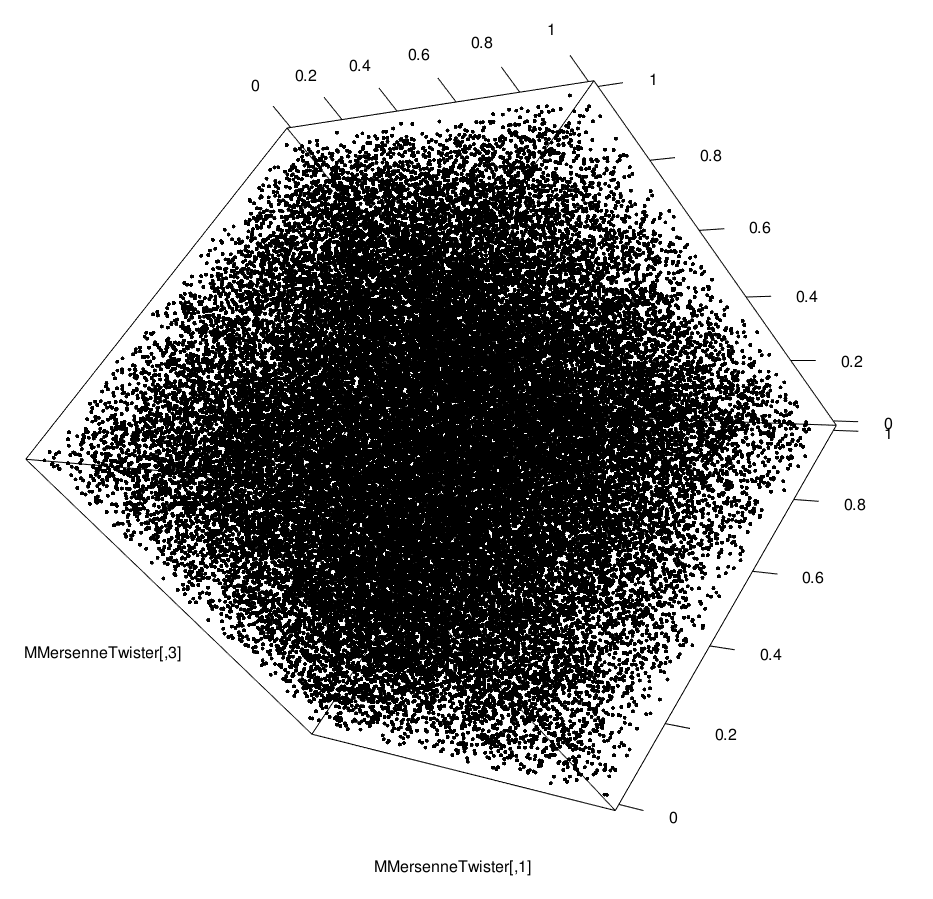
\includegraphics[width=.48\linewidth]{MT3D}}
\subfigure[Segunda perspectiva\label{MTb}]{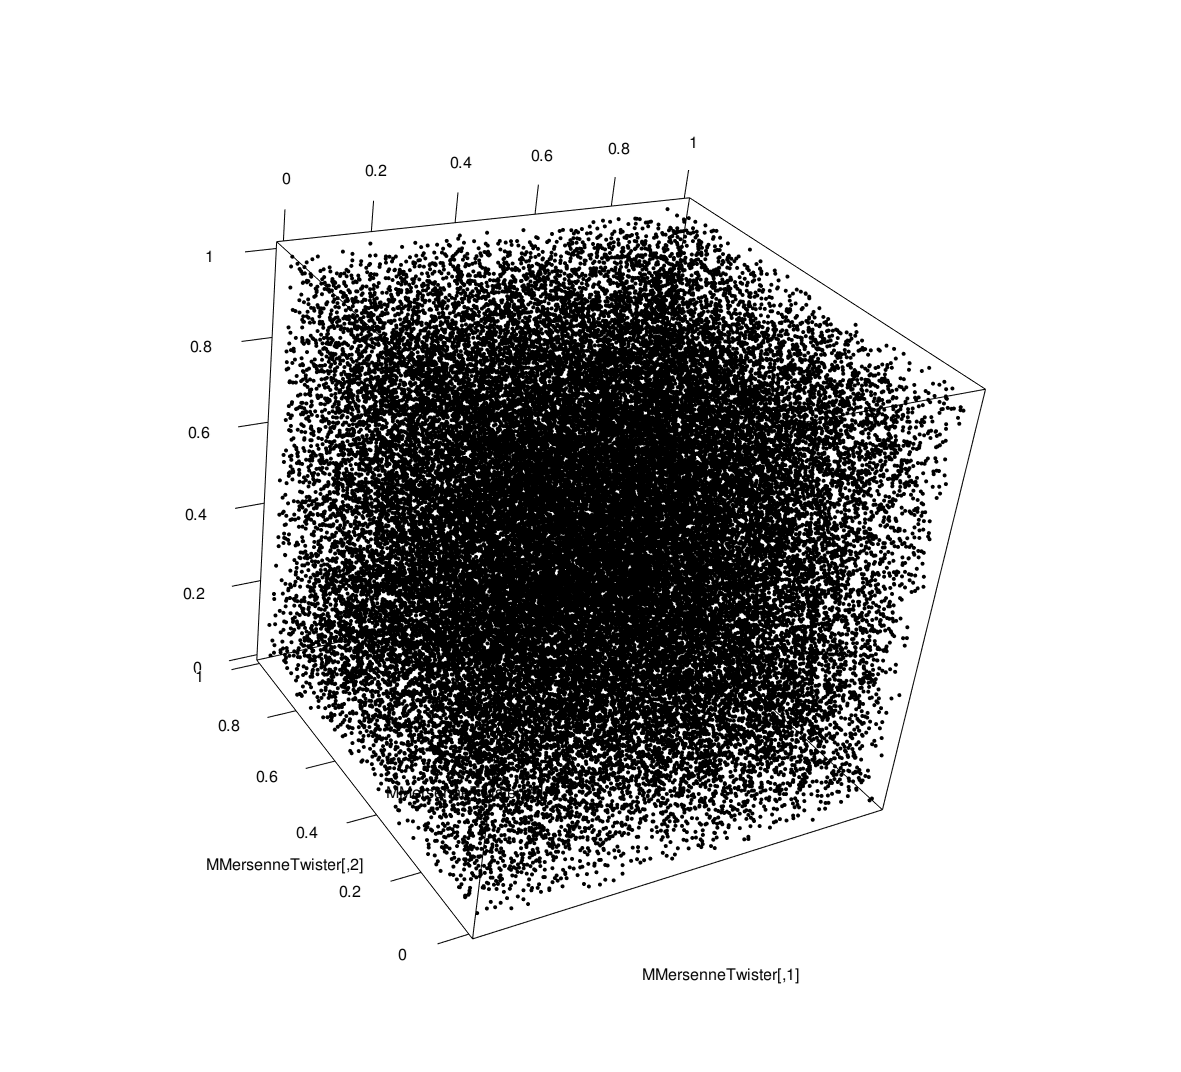
\includegraphics[width=.48\linewidth]{MT3Dsubspace}}
\caption{Visualização 3D de sequências disjuntas produzidas pelo gerador Mersenne-Twister}\label{fig:3DMT}
\end{figure}

\begin{figure}[hbt]
\centering
\subfigure[Primeira perspectiva\label{Ra}]{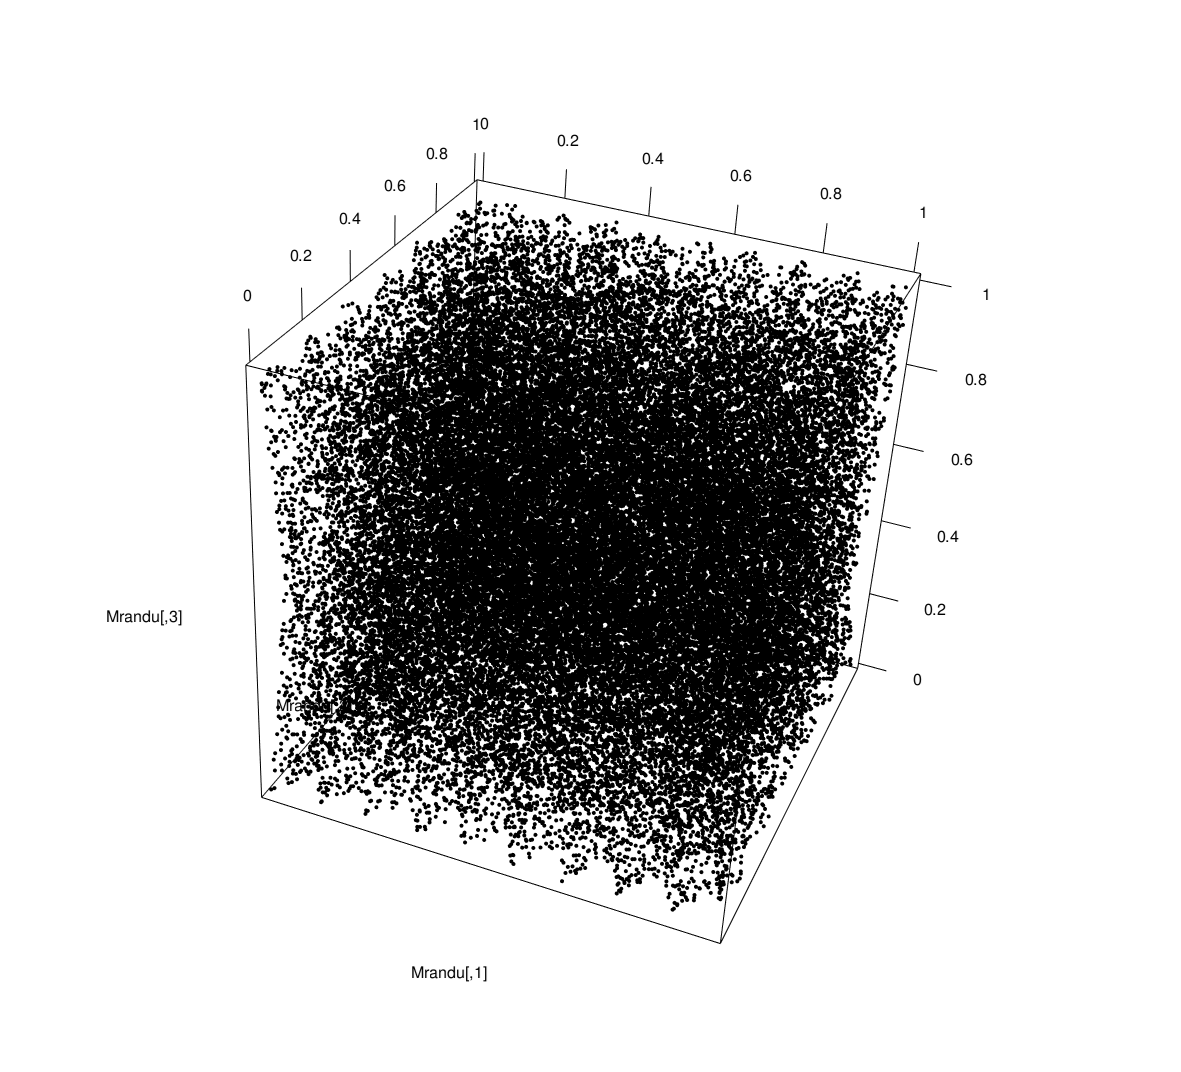
\includegraphics[width=.48\linewidth]{Randu3D}}
\subfigure[Segunda perspectiva\label{Rb}]{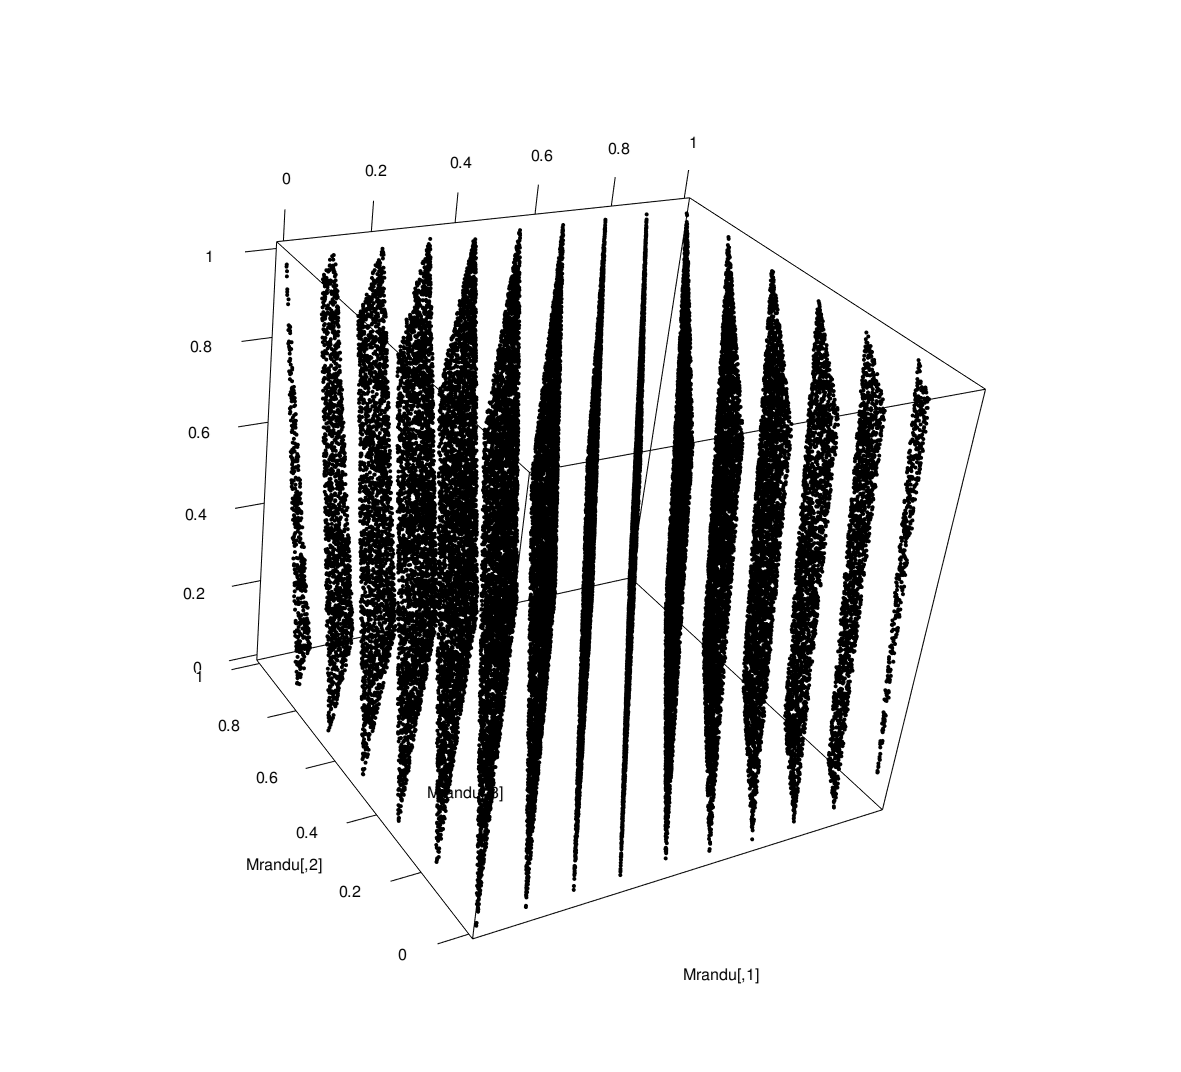
\includegraphics[width=.48\linewidth]{Randu3Dsubspace}}
\caption{Visualização 3D de sequências disjuntas produzidas pelo gerador RANDU}\label{fig:3DRandu}
\end{figure}

Embora o exemplo mostre claramente que o gerador RANDU apresenta problemas, nem sempre é fácil identificar esse tipo de estrutura.
Isso se deve a que ela pode ocorrer em espaços de dimensão maior, ou seguindo estruturas mais complexas.

\subsection{Descritores baseados em Teoria da Informação}

O trabalho pioneiro de \citet{PermutationEntropyBandtPompe} representa uma mudança de paradigma na análise de séries temporais, e será o nosso marco referencial teórico.

Eles propõem uma técnica não-paramétrica de análise de sequências que consiste em transformar palavras de $D$ dados não necessariamente subsequentes em símbolos ordinais.
Esses símbolos codificam a ordem que as $D$ observações têm na sequência e, portanto, são bem menos sucetíveis a contaminação dos que os próprios valores.
Forma-se então um histograma de proporções dos símbolos observados, e calculam-se duas quantidades: a Entropia e a Divergência de Jensen-Shannon a uma distribuição de referência (usualmente a uniforme).
A série, finalmente, é representada pelo par de valores Entropia-Complexidade Estatística, sendo que esta última é o produto da Entropia e a Divergência de Jensen-Shannon.

O conjunto de valores possíveis dos pontos característicos de qualquer série não varre $\mathbbm R^2$, mas constitui-se em um subconjunto compacto do plano: o plano Entropia-Complexidade.
Uma grande quantidade de trabalhos mostra que a posição dos pontos característicos no plano Entropia-Complexidade é capaz de caracterizar diversos tipos de dinâmicas, sendo as duas extremas o ponto $(0,1)$, que corresponde a sequências determinísticas, e o ponto $(1,0)$, típico de ruído branco.

Alguns dos trabalhos emblemáticos que empregam essa abordagem são:
\begin{description}
\item[\citet{RandomNumberGeneratorsCausality}] mostram que o plano Entropia-Complexidade permite prever o resultado dos testes Diehard de qualidade de GNPA.
\item[\citet{GeneralizedStatisticalComplexityMeasuresGeometricalAnalyticalProperties}] analisam o mapa caótico logístico e discutem cotas no plano Entropia-Complexidade.
\item[\citet{EEGAnalysisWaveletInformationTools}] analisam estados do sono utilizando decomposição wavelet e o plano Entropia-Complexidade.

\item[\citet{De_Micco_2008}] avaliam melhorias da qualidade de sequências pseudoaleatórias.
\item[\citet{De_Micco_2009}] estudam as componentes caóticas de GNPAs.
\item[\citet{ComplexNetworksEvolution}] analisam a evolução de redes dinâmicas com descritores baseados em Teoria da Informação.
\item[\citet{DistinguishingChaoticStochasticDynamicsTimeSeriesMultiscaleSymbolicApproach}] analisam a relação entre dinâmicas caóticas e estocásticas com uma abordagem multiescala.
\item[\citet{StructuralChangesDataCommunicationWSN}] utilizam descritores de Teoria da Informação para descrever a dinâmica de redes de sensores sem fios.
\item[\citet{DistinguishingNoiseFromChaos}] caracterizam sequências com componentes caóticas e estocásticas no plano Entropia-Complexidade.
\item[\citet{CharacterizationVehicleBehaviorInformationTheory}] analisam o comportamento de veículos em larga escala em função da topologia de diversas cidades.
\item[\citet{DiagnosingDynamicsObservedSimulatedEcosystem}] analisam séries temporais de fenômenos ambientais.
\item[\citet{InformationTheoryPerspectiveNetworkRobustness}] verificam o efeito de ataques em redes complexas através de descritores no plano Entropia-Complexidade.
\item[\citet{ClassificationVerificationOnlineHandwrittenSignatures}] mostram a expressividade dos descritores de Teoria da Informação para o problema de classificação e verificação de assinaturas.
\item[\citet{CharacterizationElectricLoadInformationTheoryQuantifiers}] conseguem caracterizar o tipo de dispositivo elétrico observando o ponto no plano Entropia-Complexidade em que o histórico do seu consumo é mapeado.
\end{description}

Uma limitação de todos esses trabalhos é que os pontos no plano são atribuídos a padrões prototipicos, isto é, a modelos, de forma \textit{ad hoc}.
O autor desta dissertação só conhece um trabalho em que é feita uma análise da significância da posição de pontos característicos no plano Entropia-Complexidade: o artigo de \citet{NewPermutationEntropy}.

Nesse contexto, esta dissertação fornece regiões de confiança para uma boa diversidade de situações que permitem verificar a significância da hipótese de uma sequência aleatória ou pseudoaleatória é aderente à hipótese dela ser ruído branco.

\section{Delimitação do problema} %Delimitação do problema  

A motivação deste trabalho é o desenvolvimento de um teste baseado em Teoria da Informação para verificar a hipótese de que uma sequência é ruído branco, isto é, formada por observações de variáveis aleatórias independentes e identicamente distribuídas.
Para tanto, trabalharemos com atributos derivados da simbolização de Bandt \& Pompe.
Cada sequência sob análise será transformada em um ponto no plano Entropia-Complexidade, e será medida a sua distância ao ponto característico de sequências ideais.
Analisaremos, então, a distribuição empírica de uma variedade de situações de interesse para, finalmente, propor regiões de confiança da hipótese nula.
Por fim, analisaremos sequências com o ferramental aqui proposto.

\mychapter{Proposta}{chp:Proposta}
\lhead{PROPOSTA}

% Breve resumo do capítulo.
  \lettrine{E}{ste} capítulo tem como objetivo apresentar a proposta bem como os materiais e métodos utilizados na realização do trabalho.
  
\section{Fundamentação Teórica}

Trataremos a sequência de saída de um gerador de números pseudoaleatórios como uma série temporal.
Procuraremos por estruturas indesejadas em um gerador ideal utilizando ferramentas de Teoria da Informação.

Há diversas abordagens para a análise de séries temporais, sendo que uma das mais importantes surge a partir do trabalho de \citet{PermutationEntropyBandtPompe}.

Essa abordagem consiste em transformar a série de entrada em uma sequência de símbolos.
Feito isso, computa-se o histograma de proporções dos símbolos, e calculam-se descritores a partir dele.

A hipótese subjacente a toda análise de séries temporais é que os dados observados são o resultado da operação de um sistema causal, possivelmente sujeito a ruído observacional.
Esse sistema, ou dinâmica, é responsável pela criação de padrões através de cuja observação deseja-se inferir a respeito da dinâmica.
 
A análise de séries temporais é um ramo clássico da Estatística~\cite{BrockwellDavis91} que se divide, tipicamente, na análise nos domínios do tempo e da frequência.
Ambas abordagens empregam diretamente os valores observados e, portanto, são suscetíveis ao efeito danoso de diversos tipos de contaminação.
Uma forma de tornar as análises mais imunes a contaminação é através de técnicas robustas~\cite{BustosFraiman1984}.
Outra, mais moderna, é pelo uso de métodos não-paramétricos.
 
Há diversas ferramentas que auxiliam na análise clássica de séries temporais; na data de redação deste trabalho havia \num{238} bibliotecas para essa finalidade (ver \url{https://cran.r-project.org/web/views/TimeSeries.html}).
Para essa mesma plataforma, apenas três delas trabalham exclusivamente com técnicas não paramétricas.

Seja a série temporal $\bm x = (x_1, x_2, \dots, x_n)$.
Ao invés de analisarmos os valores, transformaremos grupos de $N$ valores (não necessariamente adjacentes) em padrões ordinais, e analisaremos a sua distribuição de frequência.
Por exemplo e sem perda de generalidade, com $N=3$ e para qualquer $i$ viável,
se $x_i<x_{i+1}<x_{i+2}$ atribuiremos a esta tripla o padrão $\pi_0$;
caso $x_i>x_{i+1}>x_{i+2}$ o padrão será $\pi_1$ e assim por diante.
Com isso, há $N!$ possíveis padrões.
Esta é conhecida como \textit{simbolização de Bandt \& Pompe}~\cite{PermutationEntropyBandtPompe}.
Forma-se, então, um histograma e, a partir dele, extraem-se quantificadores como, por exemplo, entropia, distância estocástica a uma distribuição de equilíbrio, e complexidade estatística.
 
Esta simbolização é muito resistente a vários tipos de contaminação, por exemplo, o padrão $\pi_0$ não será alterado para qualquer $k>1$ que afete de forma multiplicativa $x_{i+2}$.
Ainda que o padrão seja alterado, por exemplo se $k=-1$, a mudança será local e afetará, no máximo, $N$ padrões.
 
A análise da dinâmica subjacente a uma série temporal utilizando a simbolização de Bandt \& Pompe tem sido usada com sucesso em diversas áreas como, por exemplo, 
a discriminação entre fenómenos estocásticos e caóticos~\cite{DistinguishingNoiseFromChaos}, 
a identificação de padrões de comportamento em redes veiculares~\cite{CharacterizationVehicleBehaviorInformationTheory},
a classificação e verificação de assinaturas \textit{online}~\cite{ClassificationVerificationOnlineHandwrittenSignatures},
na análise da robustez de redes~\cite{InformationTheoryPerspectiveNetworkRobustness},
a classificação de padrões de consumo de energia elétrica~\cite{CharacterizationElectricLoadInformationTheoryQuantifiers}.

O processo de simbolização, também conhecido como particionamento de dados, representa o procedimento de distribuição dos elementos em conjuntos de símbolos capazes de fornecer a sua informação causal. 
De acordo com a abordagem de Bandt e Pompe, substituímos a série por sequências de postos, obtidos pela análise desta ao longo do tempo.

Dada uma série temporal a tempo discreto $X = {x_t:1\leq t\leq M}$ de comprimento $N$, uma dimensão $D$ e um tempo de atraso (\textit{delay}) $\tau$, o particionamento é efetuado por meio da reorganização do sistema em conjuntos seguindo os passos:
\begin{itemize}
%%% ACF Reescreva usando modo matemático sempre que necessário, e respeitando a notação
%%% Use o pacote "listings"
	\item \textbf{Composição dos grupos:} Os conjuntos, ou palavras, de comprimento $D$ e \textit{delay} $\tau$ são definidas por um segmento da série: 
	 $$ (x_{t+1},x_{t+\tau},\ldots, x_{t+D\tau}).$$ 

	\item \textbf{Formação dos padrões: } Cada palavra é então relacionada a um padrão ordinal $\pi_j$ de ordem $D$, isto é, um elemento indexado univocamente por
	$$ j\in\{1, 2,\ldots, D-1, D\}. $$
\end{itemize}

Há várias formas de atribuir palavras a símbolos; neste trabalho utilizaremos a atribuição lexicográfica, isto é, se os valores da palavra $(x_{t+1},x_{t+\tau},\ldots, x_{t+D\tau})$ são tais que, ordenados, eles têm índices crescentes $b_1,b_2,\dots,b_D$, então o padrão correspondente será $\pi=b_1b_2\dots b_D$.

Calcula-se, então, o histograma de proporções $\mathcal{H} =(p_1,\dots,p_{D!})$ dos padrões observados:
$$
p_j = \frac{1}{t-N+1} \# \{
\text{padrões } \pi_j \text{ observados}
\}.
$$

O seguinte passo consiste em calcular descritores a partir desse histograma.

Os trabalhos já citados utilizam dois descritores: a Entropia de Shannon e a Complexidade Estatística da série.

A Entropia de Shannon é definida como
$$
E(\mathcal H) = -\sum_{j=1}^{D!} p_j \log p_j,
$$
em que adotamos a convenção $0(-\infty)=0$.
Esta é uma medida da desordem ou imprevisibilidade da lei subjacente a $\mathcal H$.
Quando todas as proporções são iguais, isto é, quando se tem uma lei uniforme $p_1=\dots=p_{D!}$, então a entropia é máxima e igual a $1$.
Chamaremos a lei uniforme ``medida de referência'', e a denotaremos $\mathcal H_R$.
Quando toda a probabilidade está concentrada em um único símbolo, ou seja há um símbolo $k$ tal que $p_k=1$, então a entropia é nula.

A entropia apenas não consegue caracterizar de forma plena a dinâmica que produz a série.
Torna-se interessante, então, o uso de um outro descritor baseado em quão diferente o histograma $\mathcal H$ é de uma lei de probabilidade de referência.
A nossa referência será a lei uniforme, e a medida de distância entre elas será a distância de Jensen-Shannon:
$$
JS(\mathcal H, \mathcal H_R) = E((\mathcal H+ \mathcal H_R)/2) -\frac{1}{2}(E(\mathcal H) + E(\mathcal H_R)).
$$



\section{Regiões de Confiança no Plano Entropia-Complexidade}

Seja $\bm X = (X_1, \dots, X_n)$ uma amostra a respeito da qual temos uma conjectura que queremos verificar.
Essa conjectura é a respeito dos parâmetros que caracterizam a distribuição da amostra, ou a respeito de parâmetros que caracterizam a distribuição de atributos relacionados à distribuição da amostra.
Chamaremos ``hipótese nula'' àquela que convimos em não rejeitar a não ser que obtenhamos suficiente evidência para isso; a denotaremos $H_0$.
Por vezes precisaremos da ``hipótese alternativa'', que denotaremos $H_1$.

Classicamente, um teste de hipótese se baseia em uma estatística de teste $T$ que depende exclusivamente da amostra $\bm X$, isto é, $T(\bm X)$, e é construída de tal forma que adota valores ``pequenos'' sob $H_0$ e ``cresce'' conforme ``se afasta'' de $H_0$.
Idealmente, conhecemos a distribuição de $T$ sob a hipótese nula e, com isso, somos capazes de aferir a probabilidade de observarmos valores ``grandes'' mesmo sob $H_0$.
Definimos, assim, o $p$-valor do teste baseado em $T(\bm X)$ para o valor observado $\eta$ como $\Pr_{H_0}(T(\bm X) \geq \eta)$.
O procedimento básico consiste em rejeitar a hipótese nula ao nível de significância $100(1-\alpha)\%$ se o $p$-valor for inferior a $\alpha$, e em não rejeitá-la caso contrário.
Mais modernamente, não se fala em ``rejeição'', reporta-se o $p$-valor, deixando a decisão para o leitor. Desta forma, chamaremos de ``valor crítico'' o conjunto de valores, definidos pelo leitor tais que, quando assumidos pela estatística de teste $T$ levam à rejeição da hipótese, nula $H_0$. 

Um teste pode incorrer em dois tipos de erro, ou rejeitar a hipótese nula quando, na verdade, os dados provêm dela, ou não rejeitá-la quando os dados provêm de outro modelo.
O primeiro chama-se ``Erro Tipo~I'' ou ``Falso Positivo'', e o segundo ``Erro Tipo~II'' ou ``Falso Negativo''.
A probabilidade de incorrer no Erro Tipo~I chama-se ``Tamanho do Teste'', enquanto a probabilidade do complementar do evento que leva ao Erro Tipo~II é o ``Poder do Teste''.


% De forma análoga, utilizaremos o termo ``nível de significância'' como a probabilidade máxima de $\alpha$ que nos leve a não rejeitar $H_0$ e acima da qual rejeita-se $H_0$, ou seja a probabilidade de rejeitar $H_0$ quando a mesma é verdadeira.

Diversos testes foram desenvolvidos ao longo do tempo com o objetivo de testar a aleatoriedade de sequências de números.
Como ``aleatoriedade'' é uma noção vaga, cada teste procura identificar uma ou algumas falhas dos dados.
Por esse motivo é que há classes ou conjuntos de testes que, aplicados de forma criteriosa, permitem aferir o quanto uma sequência se afasta da hipótese de aleatoriedade.
A partir dessa análise, pode se ter uma ideia do comportamento global do gerador que a produziu.

Sob a conjectura de aleatoriedade, cada estatística de teste $T$ tem uma distribuição, que pode ser determinada ou de forma exata ou de forma aproximada, mas sempre precisa ser conhecida.
Com ela é possível informar o $p$-valor de uma determinada amostra.

Não conhecemos, contudo, a distribuição conjunta do par $(E,JS)$ para uma sequência de variáveis aleatórias coletivamente independente e identicamente distribuídas segundo uma lei uniforme.
Como também não conhecemos a distribuição do par $(H,C)$ decidimos fazer a análise empírica de dados obtidos de fontes ``confiáveis''.

Para isso, utilizamos três fontes de dados: duas físicas e uma algorítmica.
As fontes físicas foram dados de medidas de estados quânticos \citep{RNGVacuumStates} (que denominaremos \textit{sequências quânticas}) e de sinais de rádio \citep{RandomHostingAdvice} (que chamaremos \textit{sequências de rádio}).
A fonte algorítmica é o gerador Mersenne-Twister \citep{Matsumoto98}, considerado um padrão de qualidade de algoritmos de geração de números pseudoaleatórios.

Obtivemos com os autores \num{54000000} de observações de cada gerador físico, e as submetemos à análise dos padrões de Bandt \& Pompe.

Obtivemos os valores de entropia e complexidade estatística para todas as sequências possíveis de tamanho \num{18000}, palavras de tamanho $D\in\{3, 4, 5, 6\}$ e \textit{lag} $\tau\in\{1, 10, 30,50\}$.

Seguindo a proposta de \citet{NewPermutationEntropy}, nossa medida de qualidade é a distância do ponto padrão observado $(E,C)$ no plano Entropia-Complexidade ao ponto ideal $(1,0)$.
Empregamos, como esse autor, a distância euclidiana.


\section{Artefatos}Para organizar, catalogar e facilitar a consulta a todo material obtido, as referências foram gerenciadas com a ferramenta \emph{JabRef}. Um gerenciador de referências bibliográficas multiplataforma gratuito que permite organizar de maneira centralizada vários vínculos entre as referências utilizadas, bem como visualizar e anotar as mesmas dentro da própria ferramenta. Quanto à editoração eletrônica do trabalho, fez-se uso da plataforma \LaTeX, com editor de textos \emph{TeXstudio} de código aberto. Este trabalho foi desenvolvido num equipamento com as configurações constantes na tabela~\ref{local_env}.

Adicionalmente, para o processamento dos dados das sequências, foi utilizado a infraestrutura computacional do Laboratório de Computação Científica e Análise Numérica da Universidade Federal de Alagoas \textit{LaCCAN-UFAL}, descrito na tabela~\ref{virt_env}.

\begin{table}[hbt]
\centering
\caption{Ambiente local utilizado no desenvolvimento do trabalho}\label{local_env}
\begin{tabular}{c|c}
	\toprule
	Arquitetura & Intel core $i5$ $2,4$ GHz $64$ bits - $8$GB RAM\\
	\midrule
	S.O. & MacOS High Sierra $10.13$ \\
	\midrule
	Ambiente R & R v$3.4.2$ e RStudio v$1.0.153$\\
	\midrule
	\LaTeX & MacTeX v$2017$ e TeXstudio v$2.1.3$\\
	\bottomrule
\end{tabular}
\end{table}


\begin{table}[hbt]
\centering
\caption{Ambiente remoto virtual utilizado no desenvolvimento do trabalho}\label{virt_env}
\begin{tabular}{c|c}
	\toprule
	Arquitetura & Intel Xeon $E312xx$ 16 Cores 32GB RAM\\
	\midrule
	S.O. & Debian 8 GNU/Linux Kernel v$3.16.0-4-amd64$\\
	\midrule
	Ambiente R & R v$3.4.1$ - ``Single Candle''\\
	\bottomrule
\end{tabular}
\end{table}


Do ponto de vista técnico deste trabalho, foi utilizada a plataforma de análise estatística R. 
Esta plataforma foi desenvolvida originalmente por Ross Ihaka e Robert Gentleman, com o intuito de ser uma linguagem de código aberto voltada para a análise estatística e, consequentemente, a precisão numérica com fortes características funcionais \citep{Rmanual}. 
Por este motivo, ela será utilizada para a geração e manipulação das sequências pseudoaleatórias, análise dos dados e geração dos gráficos desse trabalho. A precisão numérica desta ferramenta, sendo aferida por \citet{Almiron:09}, é adequada para essa abordagem.

As ferramentas utilizadas no desenvolvimento deste trabalho, são preferencialmente multiplataforma e código aberto com licença de uso \emph{GNU General Public License}~(GPL).

Todos esses aplicativos, métodos e informações obtidas, forneceram grandes contribuições para o traçado da linha mestra deste trabalho, indicando que o mesmo está na fronteira do conhecimento produzindo um estado da arte fidedigno aos temas e ferramentas adotadas para norteá-lo.

\mychapter{Resultados}{chp:resultados}
\lhead{RESULTADOS}


Trabalhamos com sequências de observações provindas de três geradores: dois físicos (considerados ``verdadeiramente aleatórios'') e um algorítmico (o gerador Mersenne-Twister, que é reputado um dos melhores geradores pseudoaleatórios).

Para cada gerador considerado coletamos sequências disjuntas de tamanho \num{1000} e \num{50000}, de cada tamanho de palavra $D$ e a cada \textit{lag} $\tau$.
Temos, assim, quatro fatores a serem analisados.

Cada sequência passou pelo processo de simbolização, e foi calculado o histograma dos símbolos.
Foram então calculados os valores de Entropia e de Complexidade de cada histograma, bem como a distância euclidiana desses valores ao ponto de referência $(1,0)$.

O primeiro passo consistiu em fazer uma análise visual das distâncias dentro do plano $(H,C)$.
Dessa análise visual concluímos que é plausível eliminar o fator gerador e, para tanto, aplicamos o teste de Kolmogorov-Smirnov aos pares de distâncias oriundas de distâncias comparáveis, isto é, provindas dos mesmo fatores $N$, $D$ e $\tau$.

Os testes de Kolmogorov-Smirnov não nos fazem rejeitar a hipótese de que os diferentes geradores produzem sequências com idênticas propriedades no que diz respeito à distância ao ponto de referência.
Assim, nos passos seguintes analisamos o agregado das distâncias provindas dos três geradores considerados.

Acompanhando a análise realizada por \citet{NewPermutationEntropy}, calculamos os quantis de ordem $999/1000$, $1/100$, $5/100$ e $10/100$ das distâncias agrupadas pelos fatores relevantes ($N$, $D$ e $\tau$).
Com isso, produzimos intervalos de confiança para testar a hipótese de que a
distância do ponto característico de uma sequência é compatível com a de uma sequência de ruído branco.
No repositório associado a esta dissertação deixamos disponíveis as funções de distribuição acumuladas dessas distâncias, com as quais é possível calcular o $p$-valor, e não apenas a decisão binária ``rejeita'' ou ``não rejeita''.

\section{Análise global das sequências}

Em todos os casos os pontos foram desenhados com \SI{1}{\percent} de transparência, para evidenciar as regiões mais e menos densas.

As figuras~\ref{Fig:ScatterAll_Quant_1k} e~\ref{Fig:ScatterAll_Quant_50k} mostram os planos Entropia-Complexidade com as respectivas curvas de complexidade mínima e máxima para cada par $D\in\{3, 4, 5, 6\}$ (colunas) e $\tau\in\{1, 10, 30, 50\}$ (linhas), com os \num{52429} pontos observados a partir das sequências obtidas pelo gerador quântico tomando $1.000$ e $50.000$ sequências respectivamente.


\begin{figure}[hbt]
	\centering
	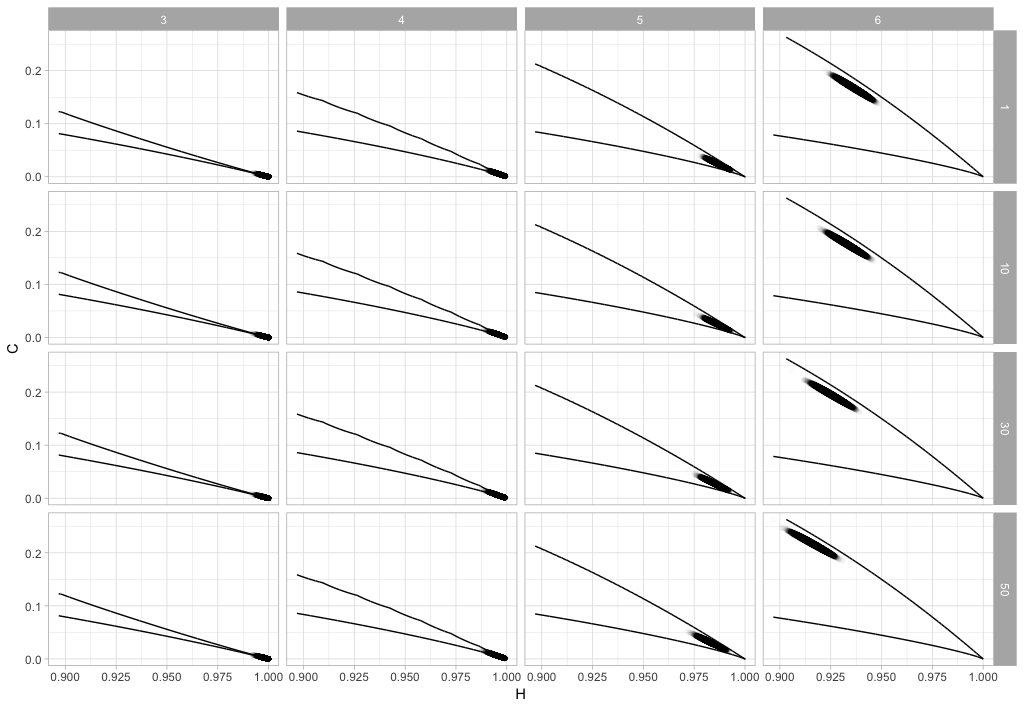
\includegraphics[width=\linewidth]{ScatterAll_Quant_1k}
	\caption{Diagramas de dispersão das sequências quânticas com $1.000$ observações para $D\in\{3, 4, 5, 6\}$ (colunas) e $\tau\in\{1, 10, 30, 50\}$ (linhas), com curvas de complexidade mínima e máxima no plano Entropia-Complexidade.}\label{Fig:ScatterAll_Quant_1k}
\end{figure}

\begin{figure}[hbt]
	\centering
	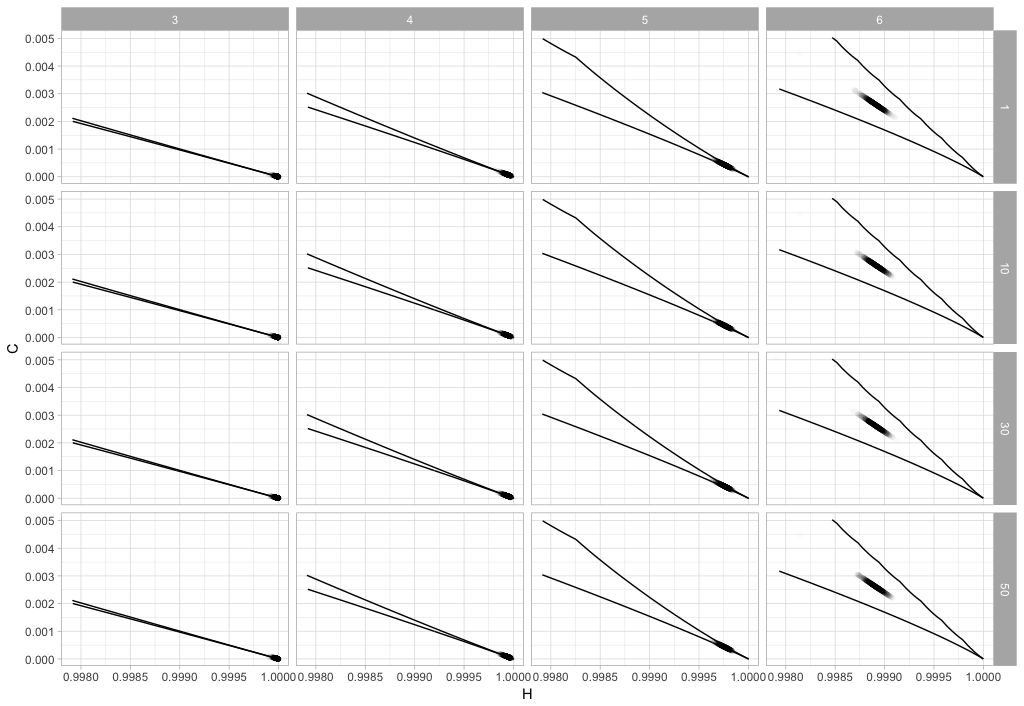
\includegraphics[width=\linewidth]{ScatterAll_Quant_50k}
	\caption{Diagramas de dispersão das sequências quânticas com $50.000$ observações para $D\in\{3, 4, 5, 6\}$ (colunas) e $\tau\in\{1, 10, 30, 50\}$ (linhas), com curvas de complexidade mínima e máxima no plano Entropia-Complexidade.}\label{Fig:ScatterAll_Quant_50k}
\end{figure}

As figuras~\ref{Fig:ScatterAll_Radio_1k} e~\ref{Fig:ScatterAll_Radio_50k} mostram os planos Entropia-Complexidade com as respectivas curvas de complexidade mínima e máxima para cada par $D\in\{3, 4, 5, 6\}$ (colunas) e $\tau\in\{1, 10, 30, 50\}$ (linhas), com os \num{52429} pontos observados a partir das sequências obtidas pelo gerador de rádio tomando $1.000$ e $50.000$ sequências respectivamente.


\begin{figure}[hbt]
	\centering
	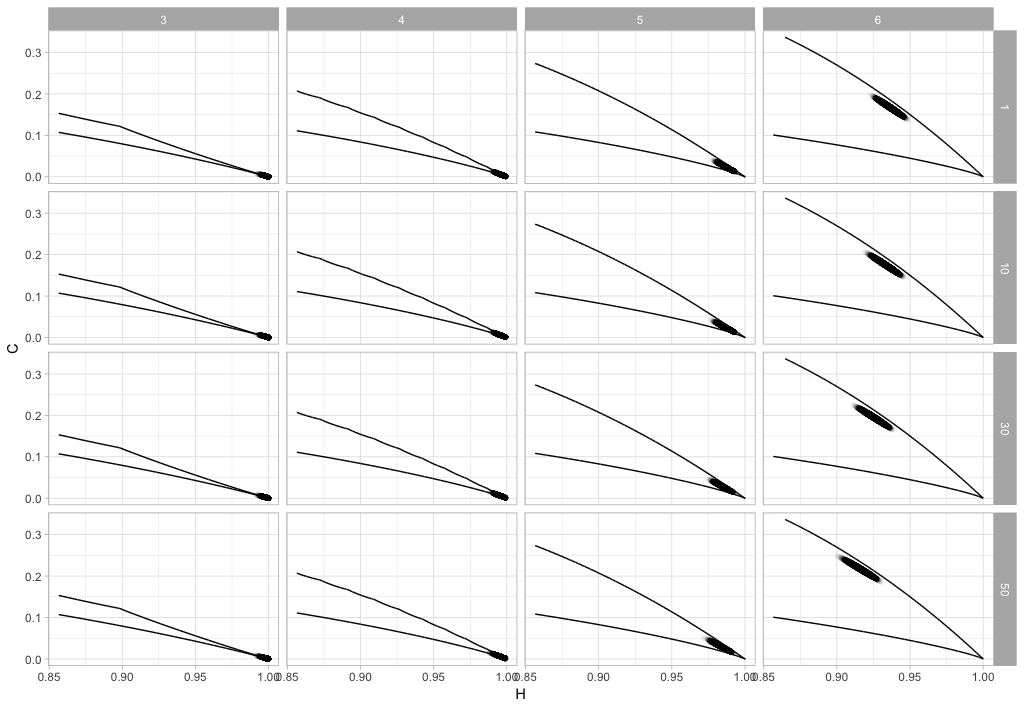
\includegraphics[width=\linewidth]{ScatterAll_Radio_1k}
	\caption{Diagramas de dispersão das sequências de rádio com $1.000$ observações para $D\in\{3, 4, 5, 6\}$ (colunas) e $\tau\in\{1, 10, 30, 50\}$ (linhas), com curvas de complexidade mínima e máxima no plano Entropia-Complexidade.}\label{Fig:ScatterAll_Radio_1k}
\end{figure}

\begin{figure}[hbt]
	\centering
	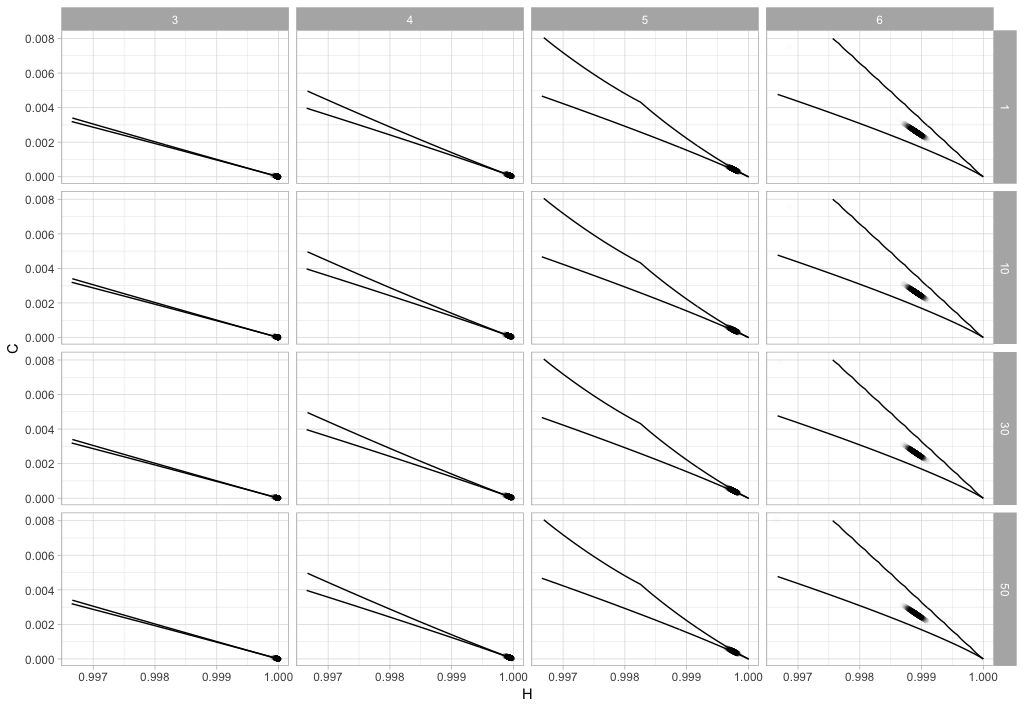
\includegraphics[width=\linewidth]{ScatterAll_Radio_50k}
	\caption{Diagramas de dispersão das sequências de rádio com $50.000$ observações para $D\in\{3, 4, 5, 6\}$ (colunas) e $\tau\in\{1, 10, 30, 50\}$ (linhas), com curvas de complexidade mínima e máxima no plano Entropia-Complexidade.}\label{Fig:ScatterAll_Radio_50k}
\end{figure}

As figuras~\ref{Fig:ScatterAll_MT_1k} e~\ref{Fig:ScatterAll_MT_50k} mostram os planos Entropia-Complexidade com as respectivas curvas de complexidade mínima e máxima para cada par $D\in\{3, 4, 5, 6\}$ (colunas) e $\tau\in\{1, 10, 30, 50\}$ (linhas), com os \num{52429} pontos observados a partir das sequências obtidas pelo gerador Mersenne-Twister tomando $1.000$ e $50.000$ sequências respectivamente.

\begin{figure}[hbt]
	\centering
	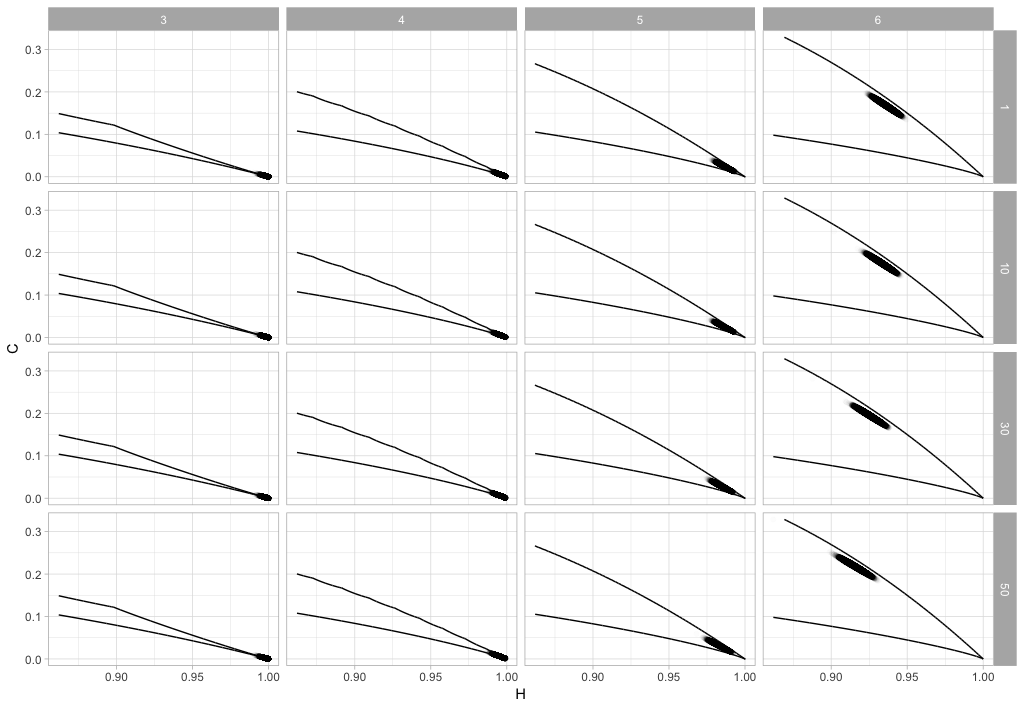
\includegraphics[width=\linewidth]{ScatterAll_MT_1k}
	\caption{Diagramas de dispersão das sequências de Mersenne-Twister com $1.000$ observações para $D\in\{3, 4, 5, 6\}$ (colunas) e $\tau\in\{1, 10, 30, 50\}$ (linhas), com curvas de complexidade mínima e máxima no plano Entropia-Complexidade.}\label{Fig:ScatterAll_MT_1k}
\end{figure}

\begin{figure}[hbt]
	\centering
	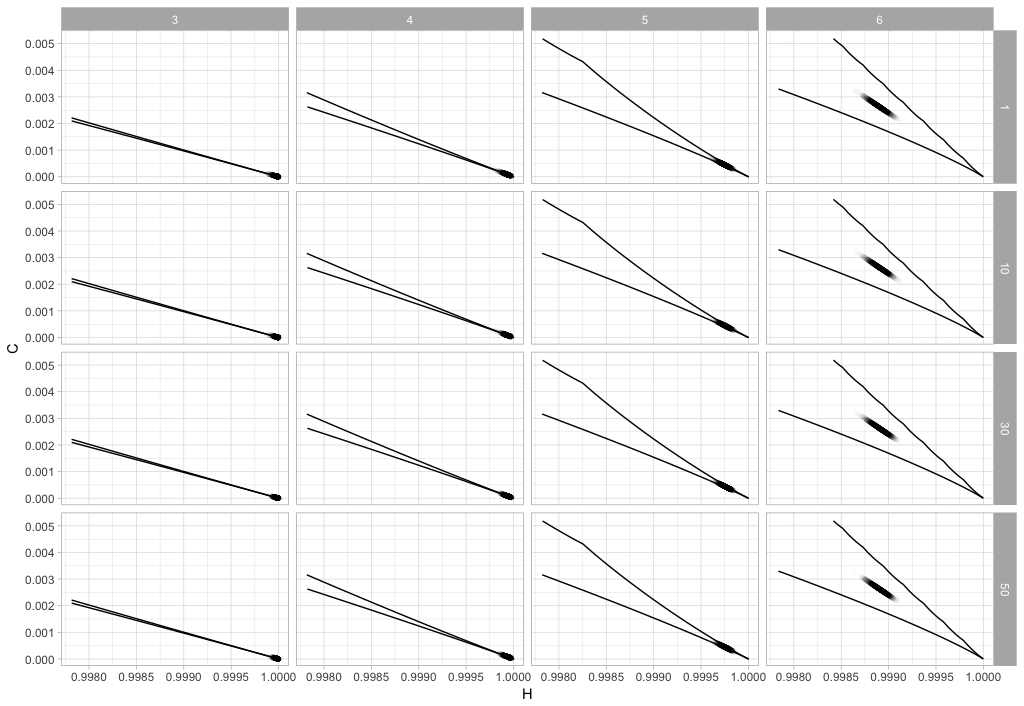
\includegraphics[width=\linewidth]{ScatterAll_MT_50k}
	\caption{Diagramas de dispersão das sequências de Mersenne-Twister com $50.000$ observações para $D\in\{3,4,5,6\}$ (colunas) e $\tau\in\{1,10,30,50\}$ (linhas), com curvas de complexidade mínima e máxima no plano Entropia-Complexidade.}\label{Fig:ScatterAll_MT_50k}
\end{figure}

A olho nu, $D$ é um fator relevante pois os diagramas de dispersão mostram comportamentos que merecem uma análise mais aprofundada, por outro lado não temos certeza de como $\tau$ e o gerador influenciam os resultados. 

As figuras~\ref{fig:GeradorIrrelevante1k} e~\ref{fig:GeradorIrrelevante50k} mostram os histogramas suavizados das distâncias para sequências de tamanho ($N=1.000$, $50.000$) respectivamente, com palavras de tamanho $D=6$  e valores de \textit{lag} ($\tau=1, 50$), sobrepondo os três geradores.
Os gráficos sugerem que o gerador é um fator irrelevante para a distribuição da distância.
Mais adiante veremos que esta impressão não se confirma totalmente.

\begin{figure} %D=6 %N 1000 t1 t 50
	\centering
		\subfigure[$D=6, \tau=1$]{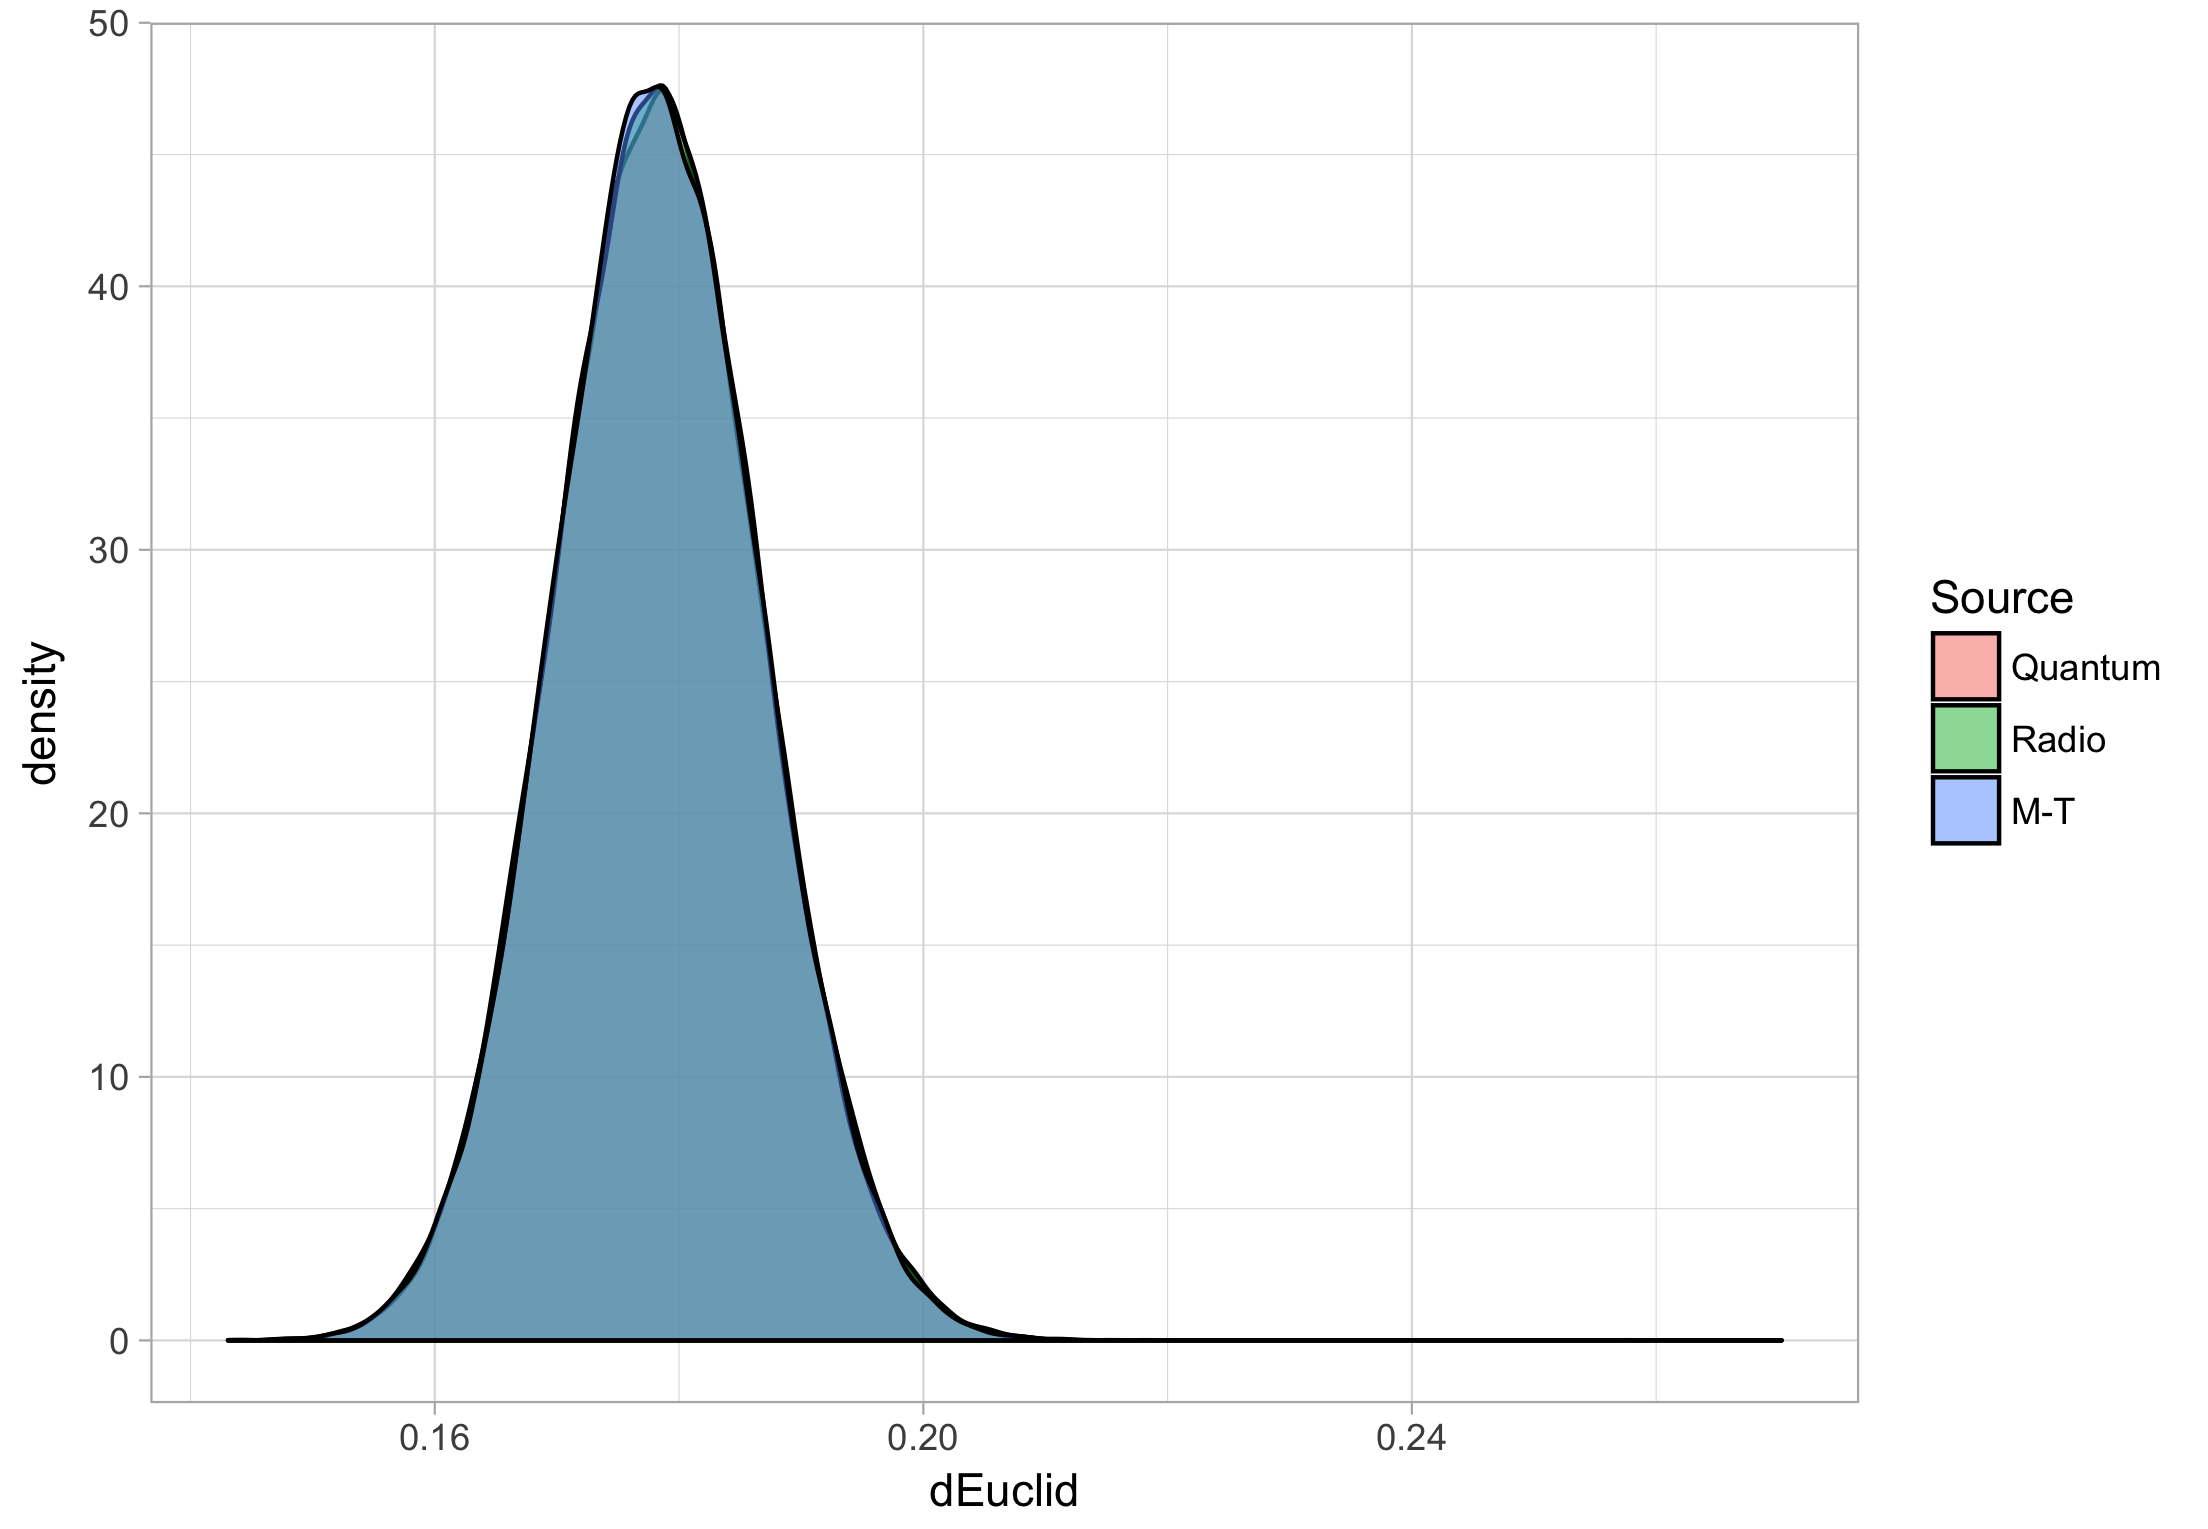
\includegraphics[width=.48\linewidth]{Hist_D6_1k_t1}}
		\subfigure[$D=6, \tau=50$]{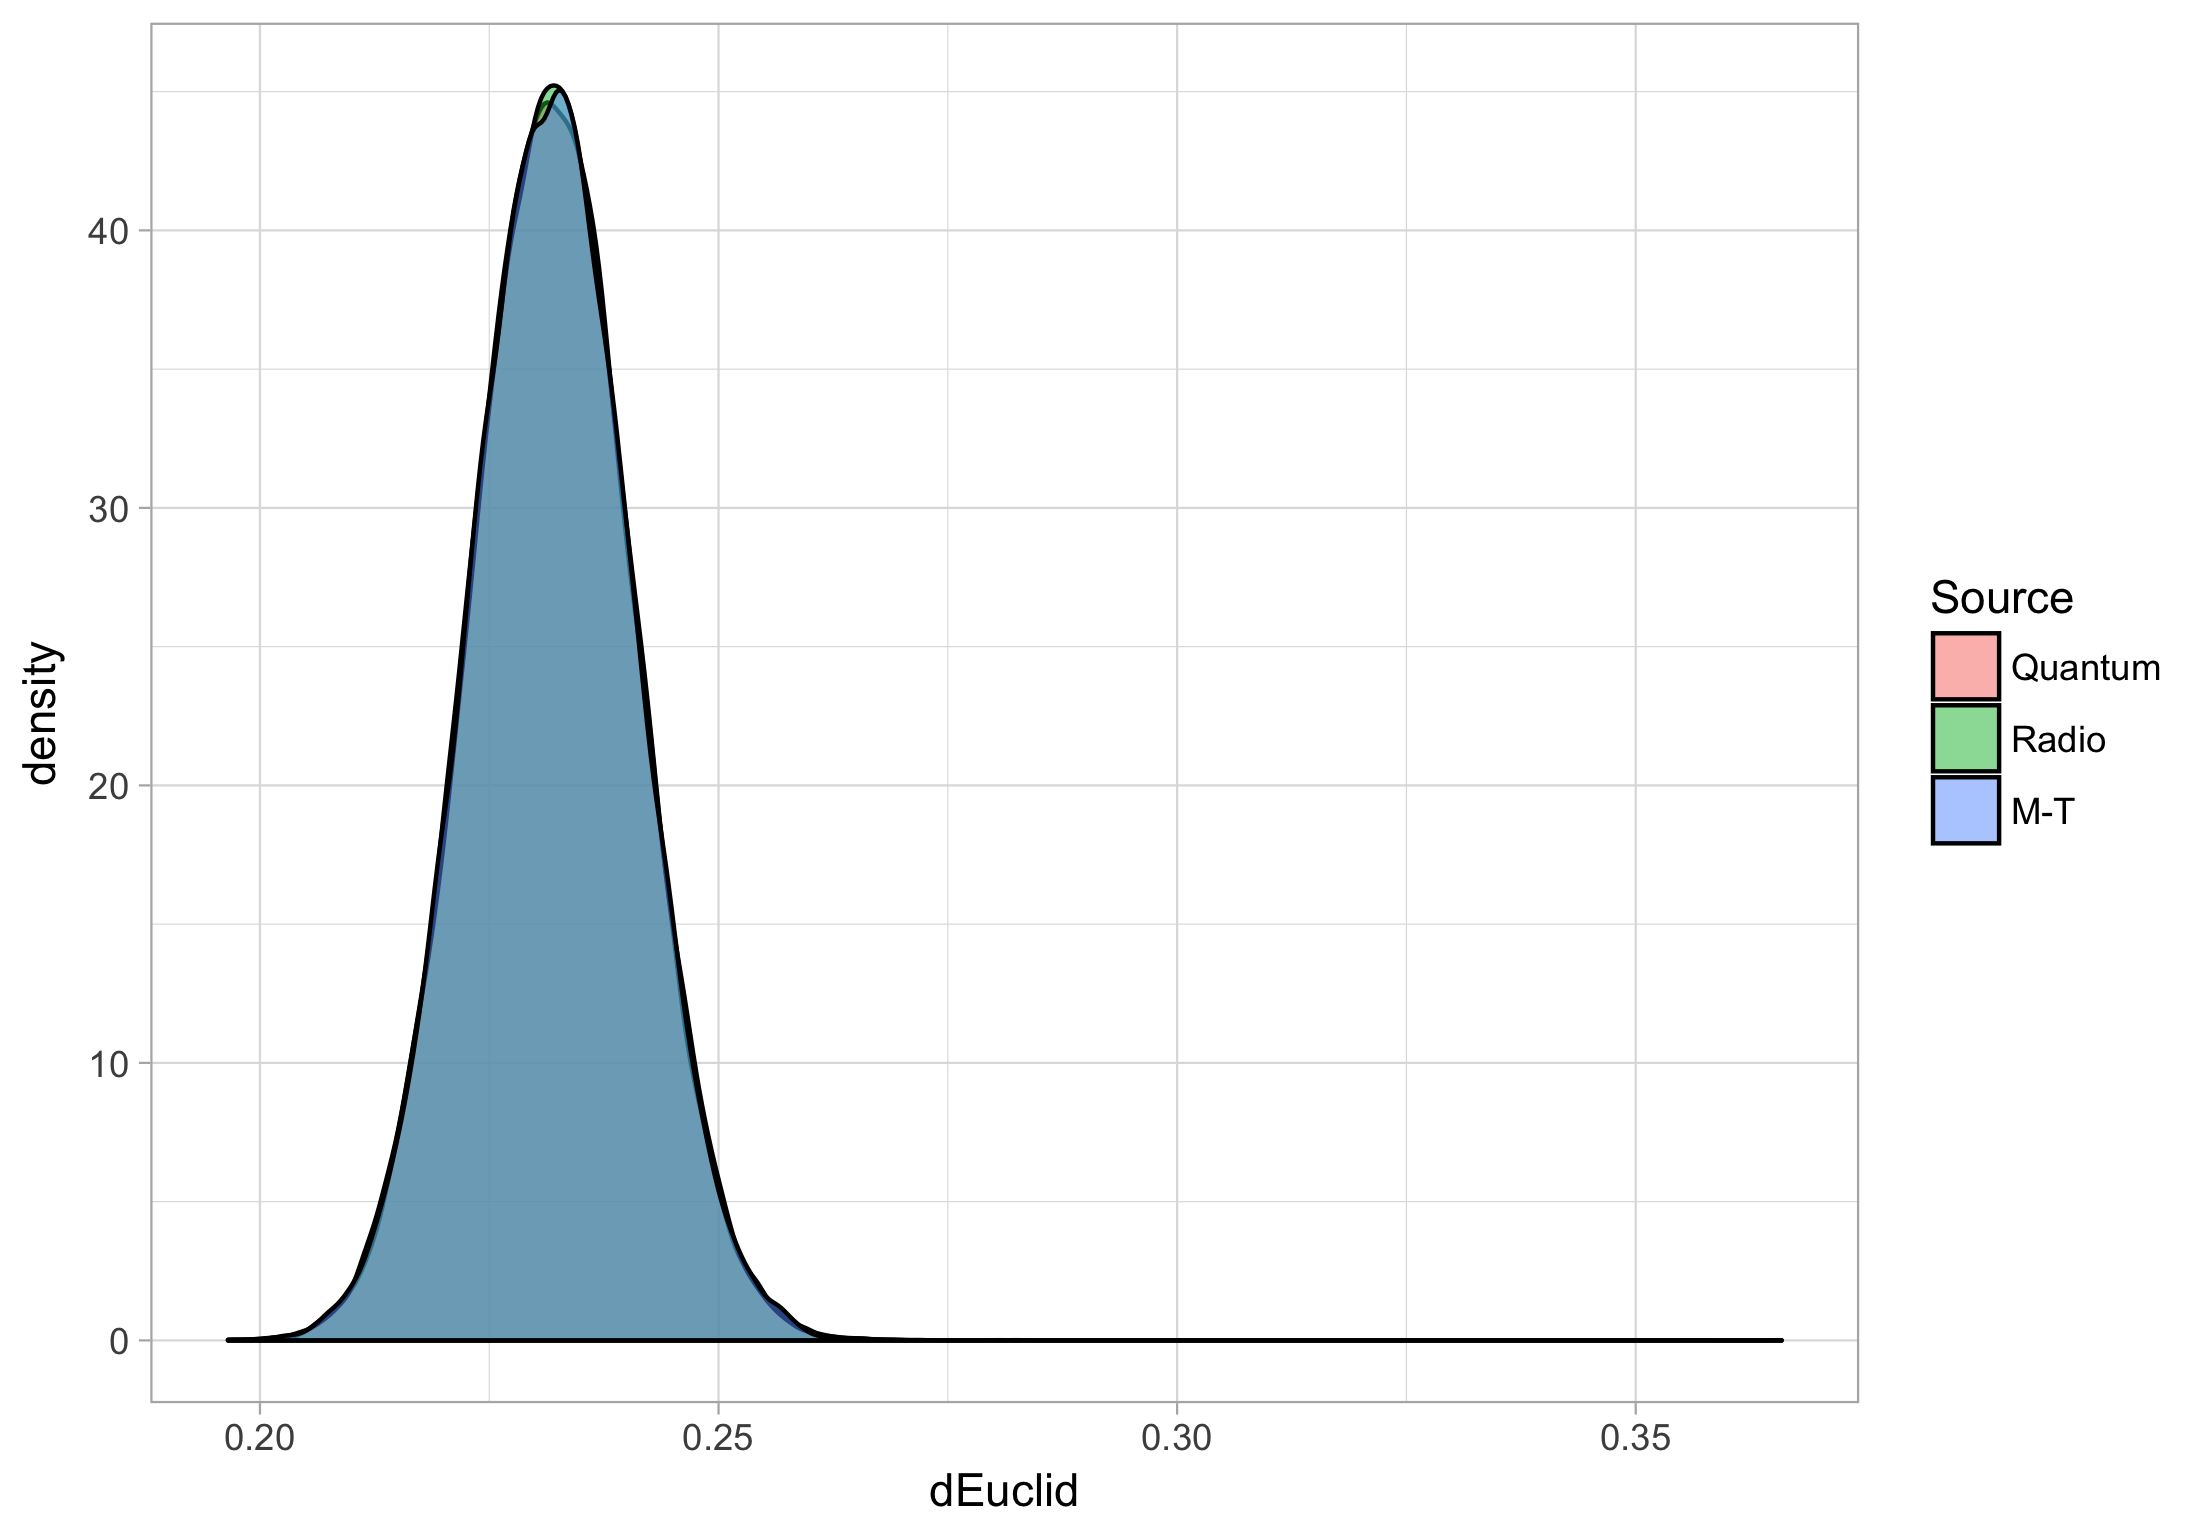
\includegraphics[width=.48\linewidth]{Hist_D6_1k_t50}}
		\caption{Histogramas suavizados de situações que sugerem que o gerador é um fator irrelevante para $N=1.000$}\label{fig:GeradorIrrelevante1k}
\end{figure}

\begin{figure} %D=6 %N 50000 t1 t 50
	\centering
		\subfigure[$D=6, \tau=1$]{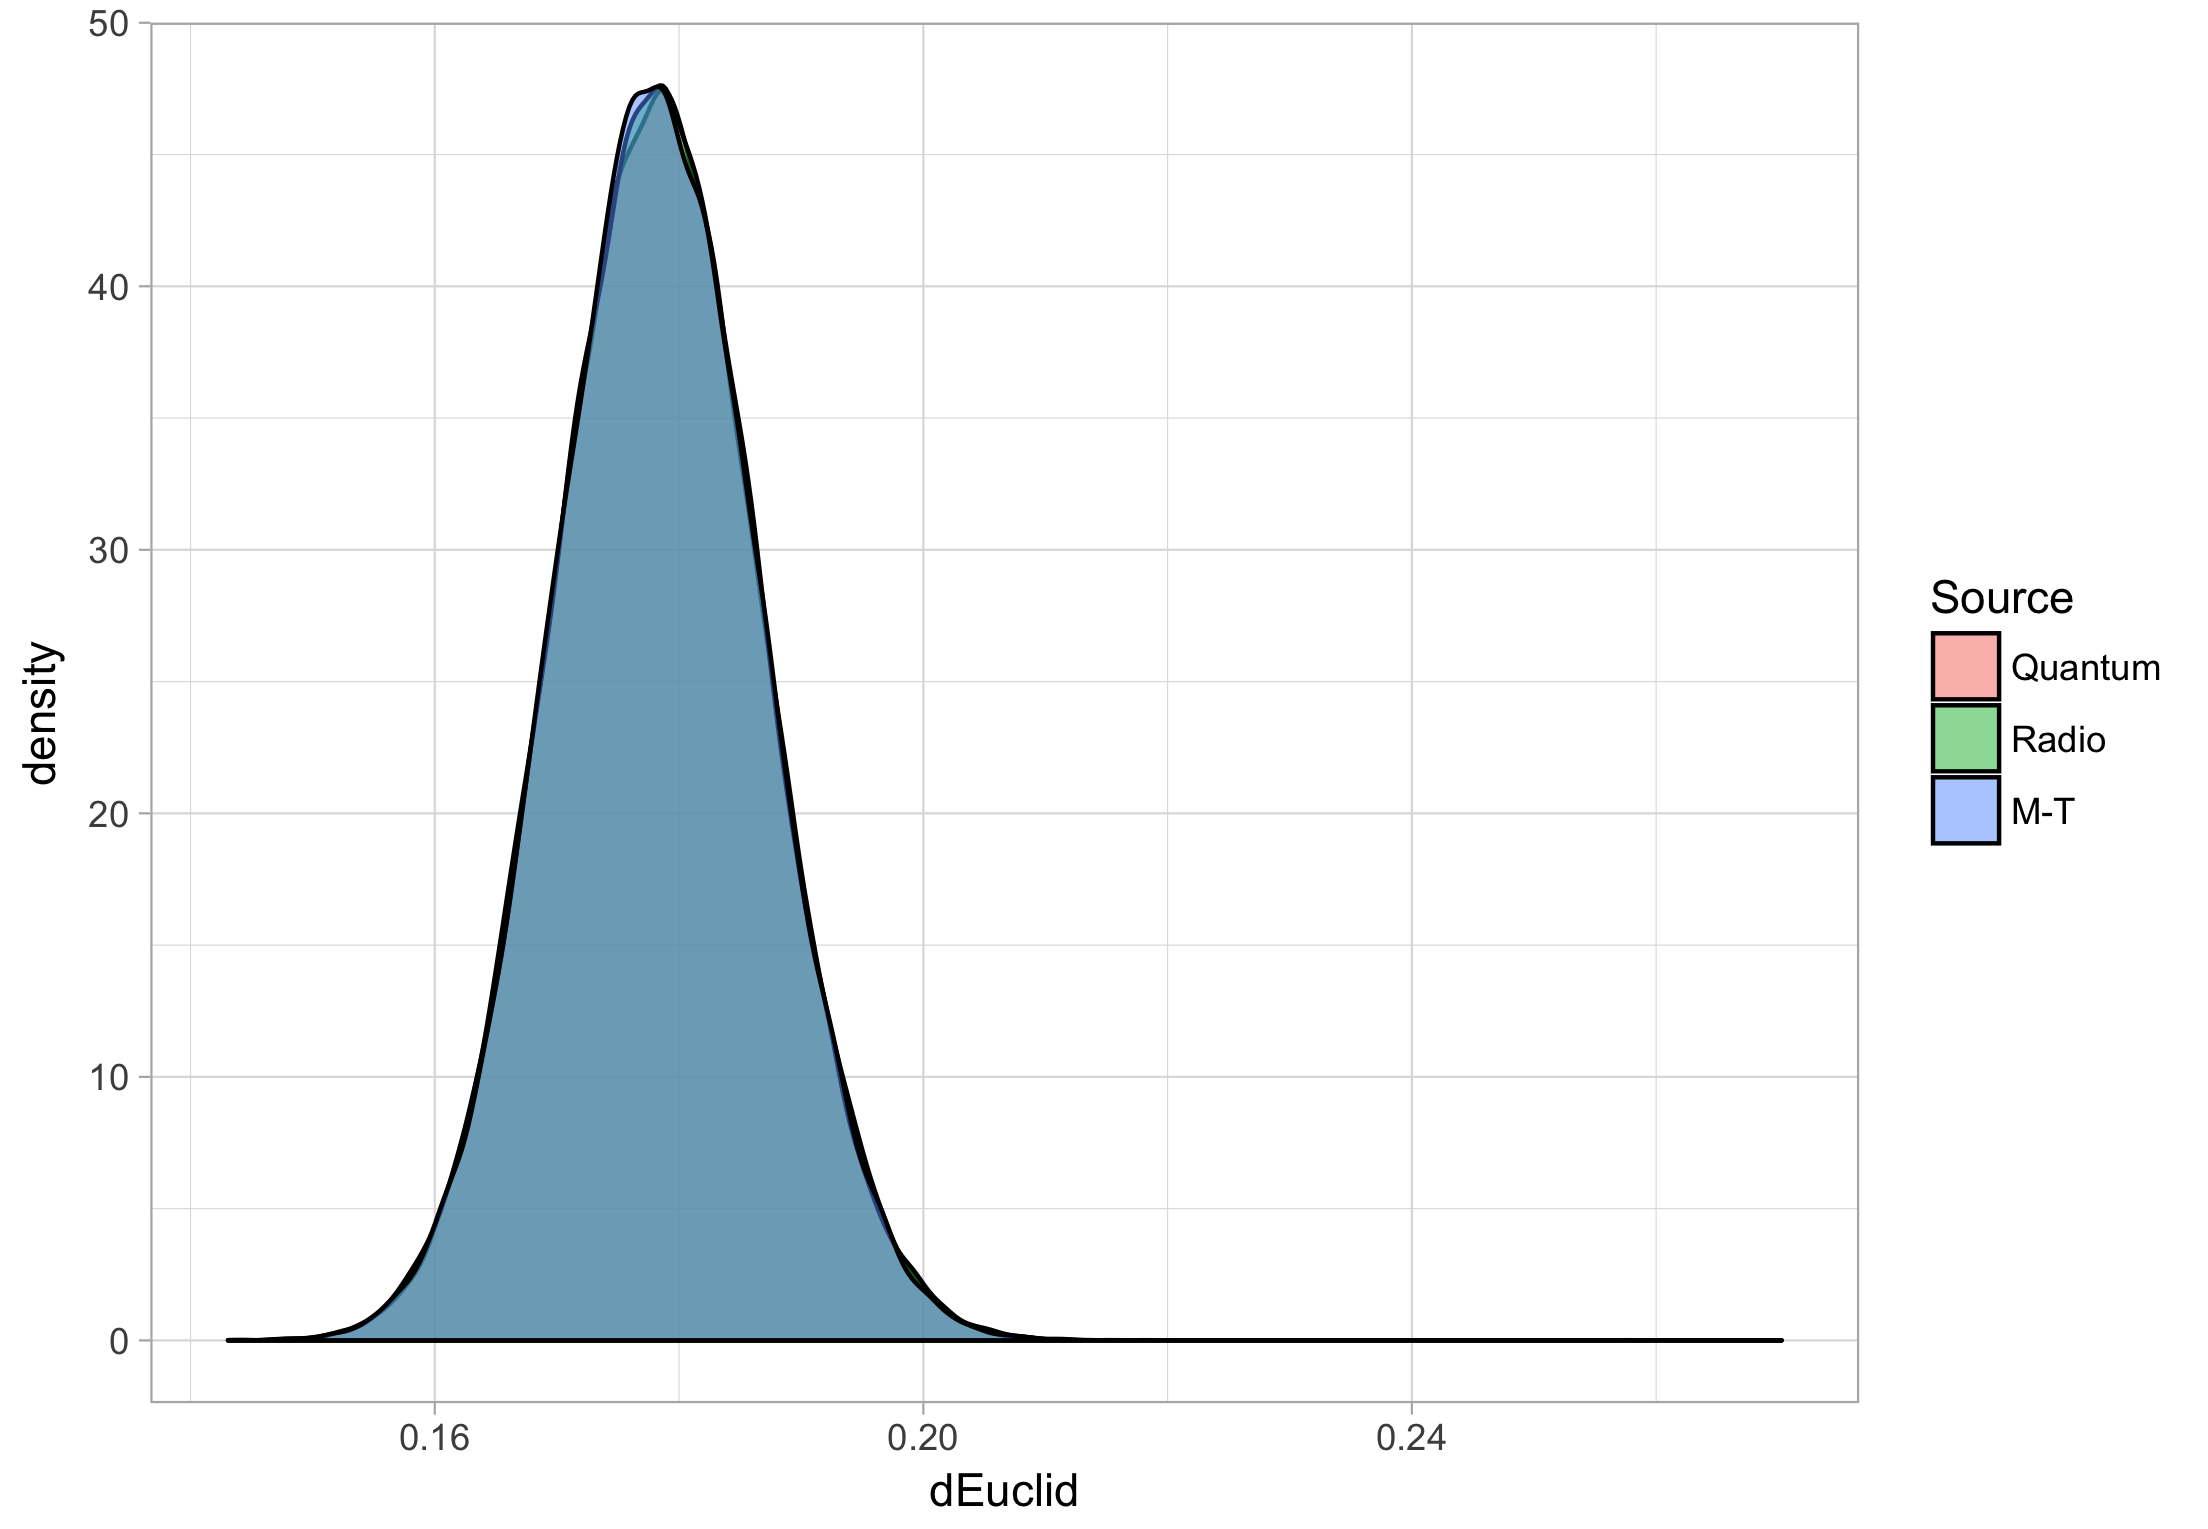
\includegraphics[width=.48\linewidth]{Hist_D6_50k_t1}}
		\subfigure[$D=6, \tau=50$]{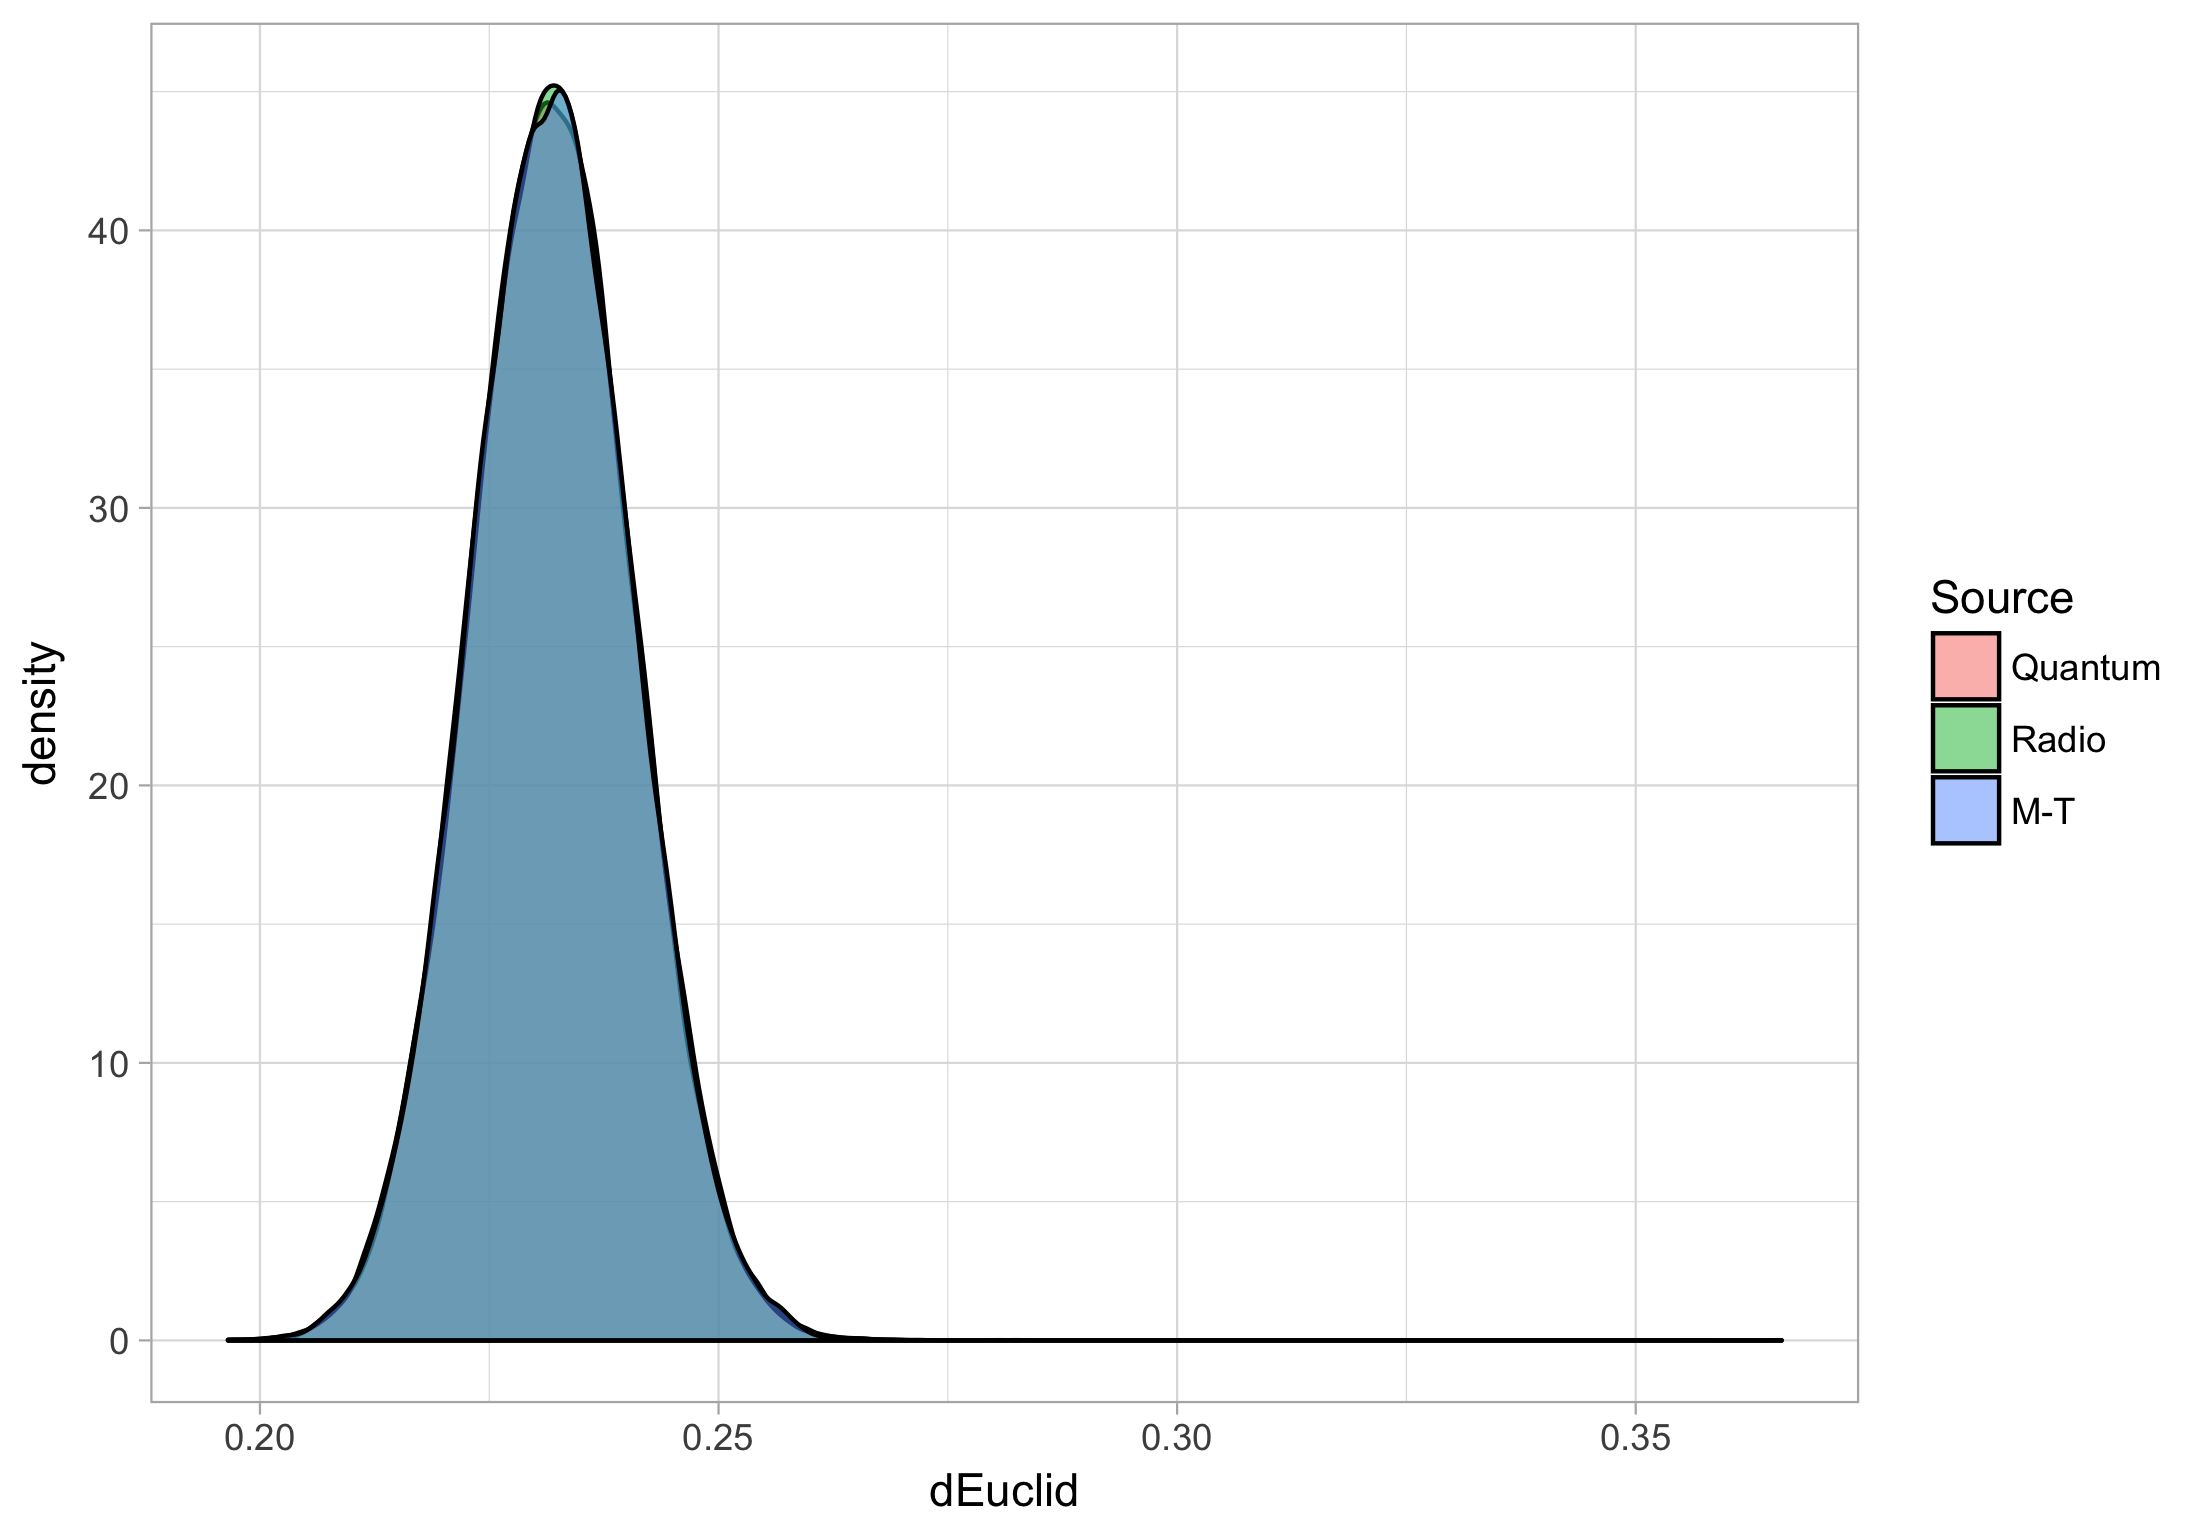
\includegraphics[width=.48\linewidth]{Hist_D6_50k_t50}}
		\caption{Histogramas suavizados de situações que sugerem que o gerador é um fator irrelevante também para $N=50.000$}\label{fig:GeradorIrrelevante50k}
\end{figure}

A figura~\ref{fig:NRelevante} mostra os histogramas suavizados das distâncias dos três geradores para palavras de tamanho $D=6$ e dois valores de \textit{lag} ($\tau=1$, $50$), sobrepondo os resultados obtidos com os dois tamanhos de sequências ($N=1.000$, $50.000$).
Os gráficos sugerem fortemente que o tamanho das sequências é um fator relevante para a distribuição da distância.

\begin{figure} %D=6 %t 1 N 1000 N 50000 (três geradores) %t 50 N 1000 N 50000 (três geradores)
	\centering
		\subfigure[$D=6$, $\tau=1$]{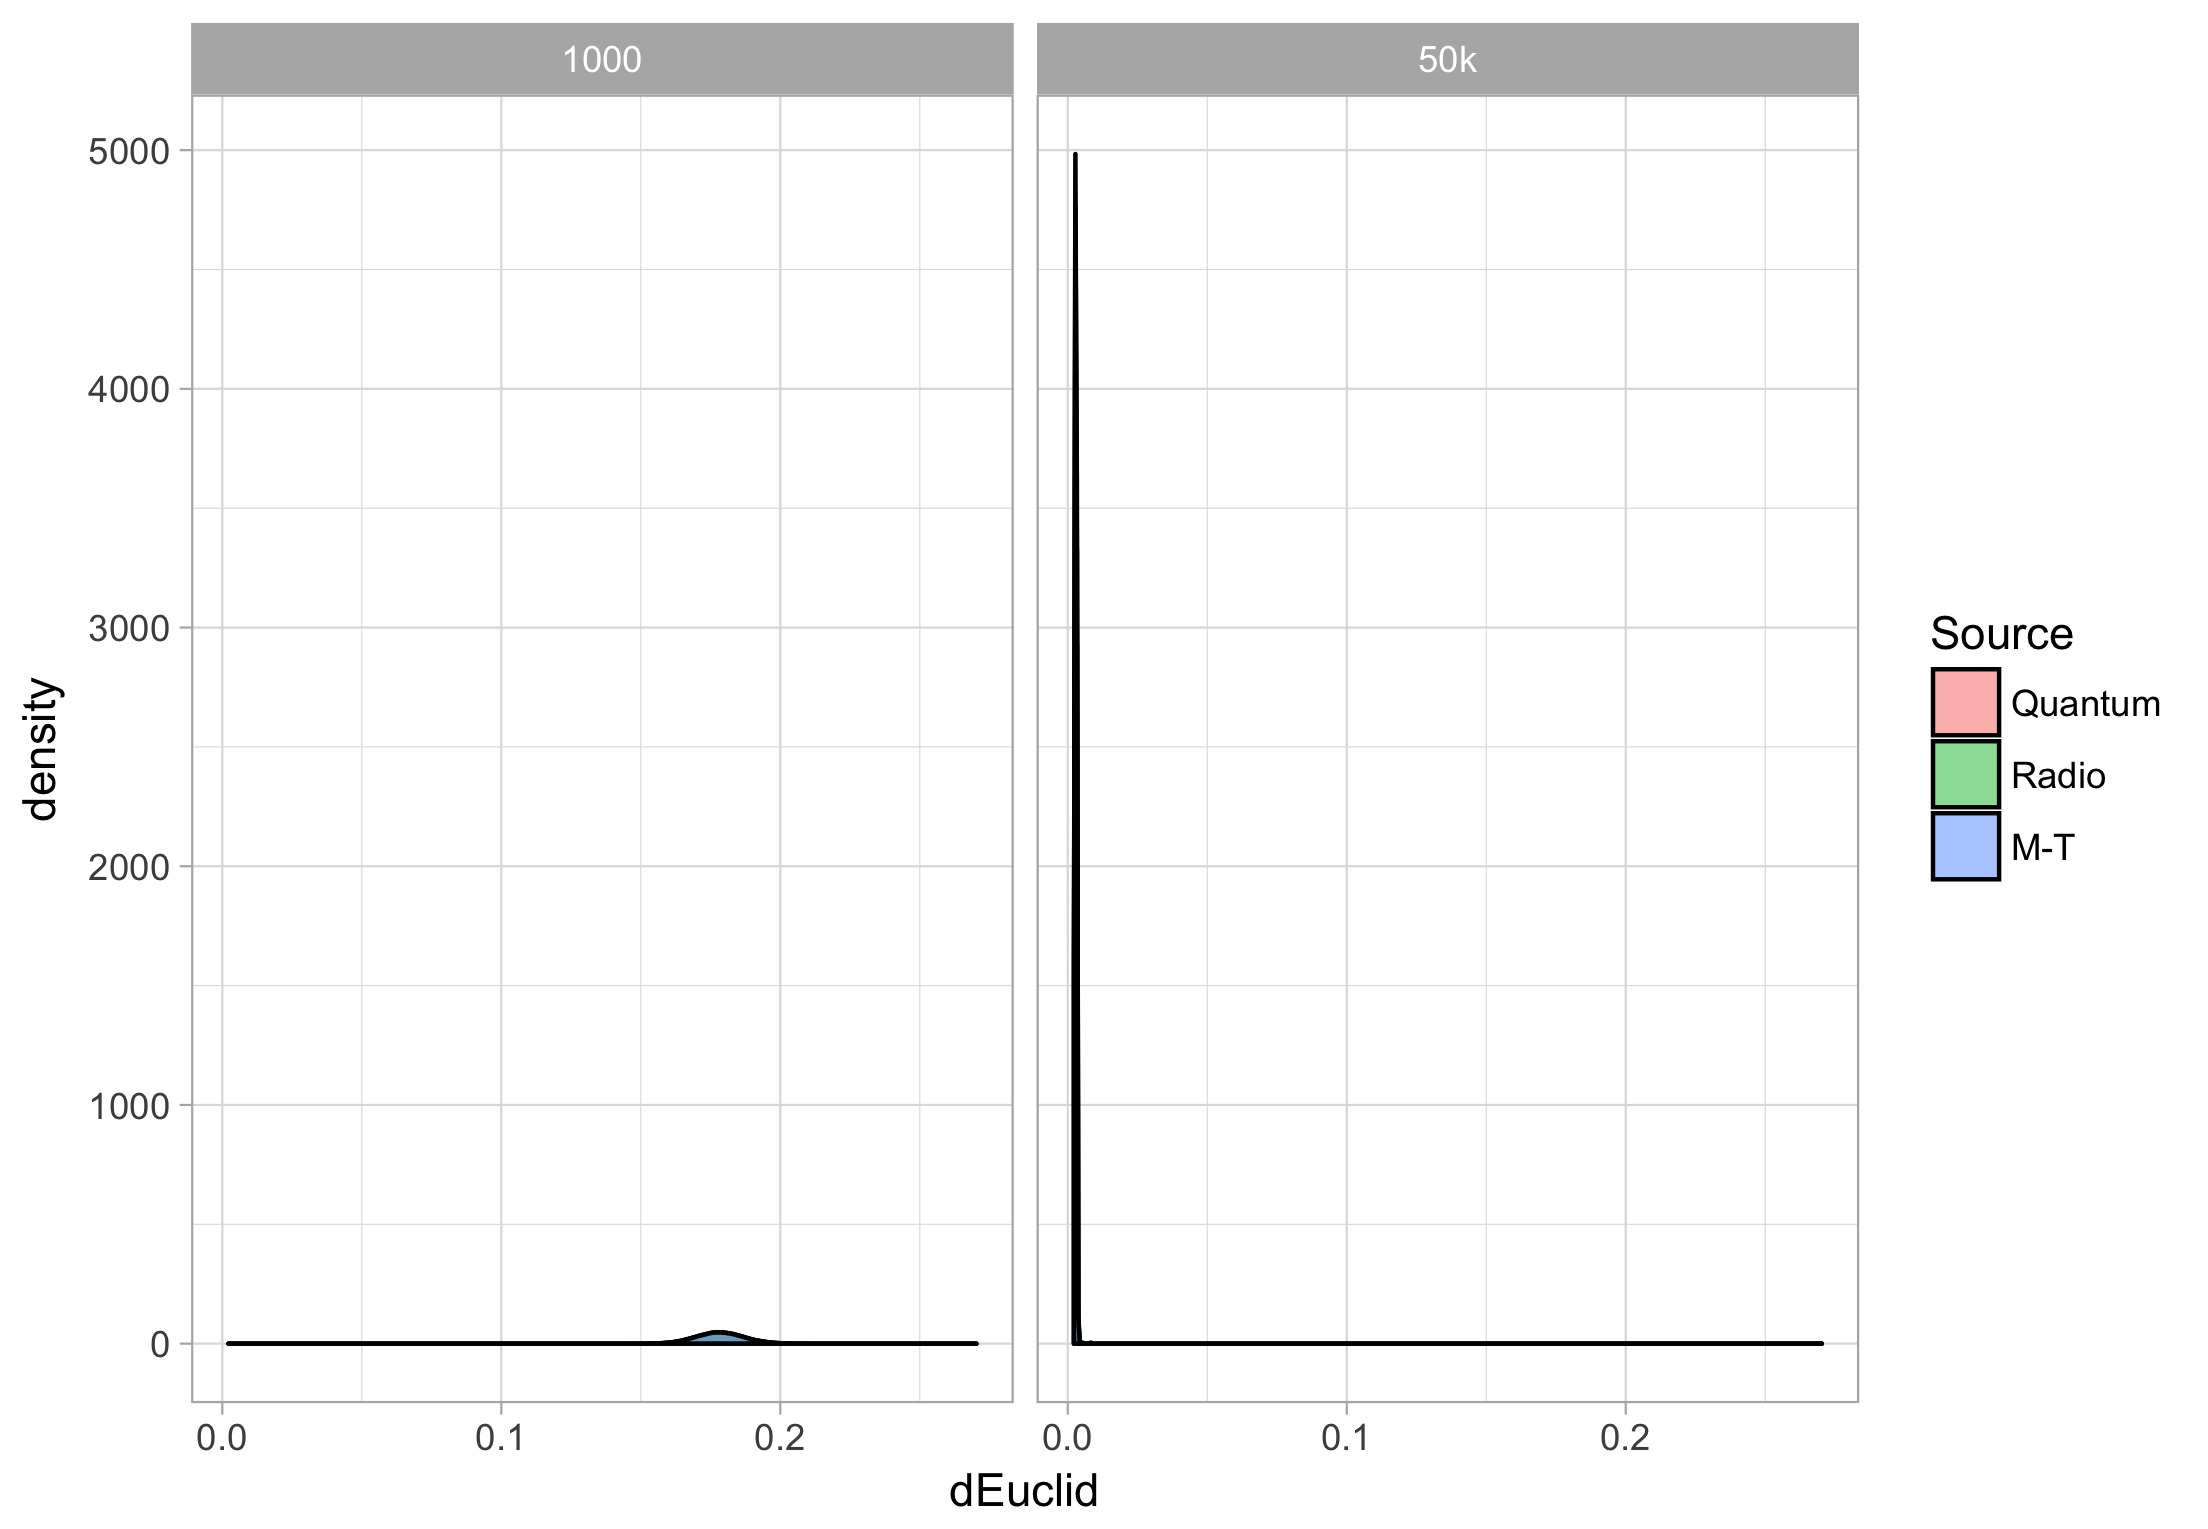
\includegraphics[width=.48\linewidth]{Hist_D6_t1}}
		\subfigure[$D=6$, $\tau=50$]{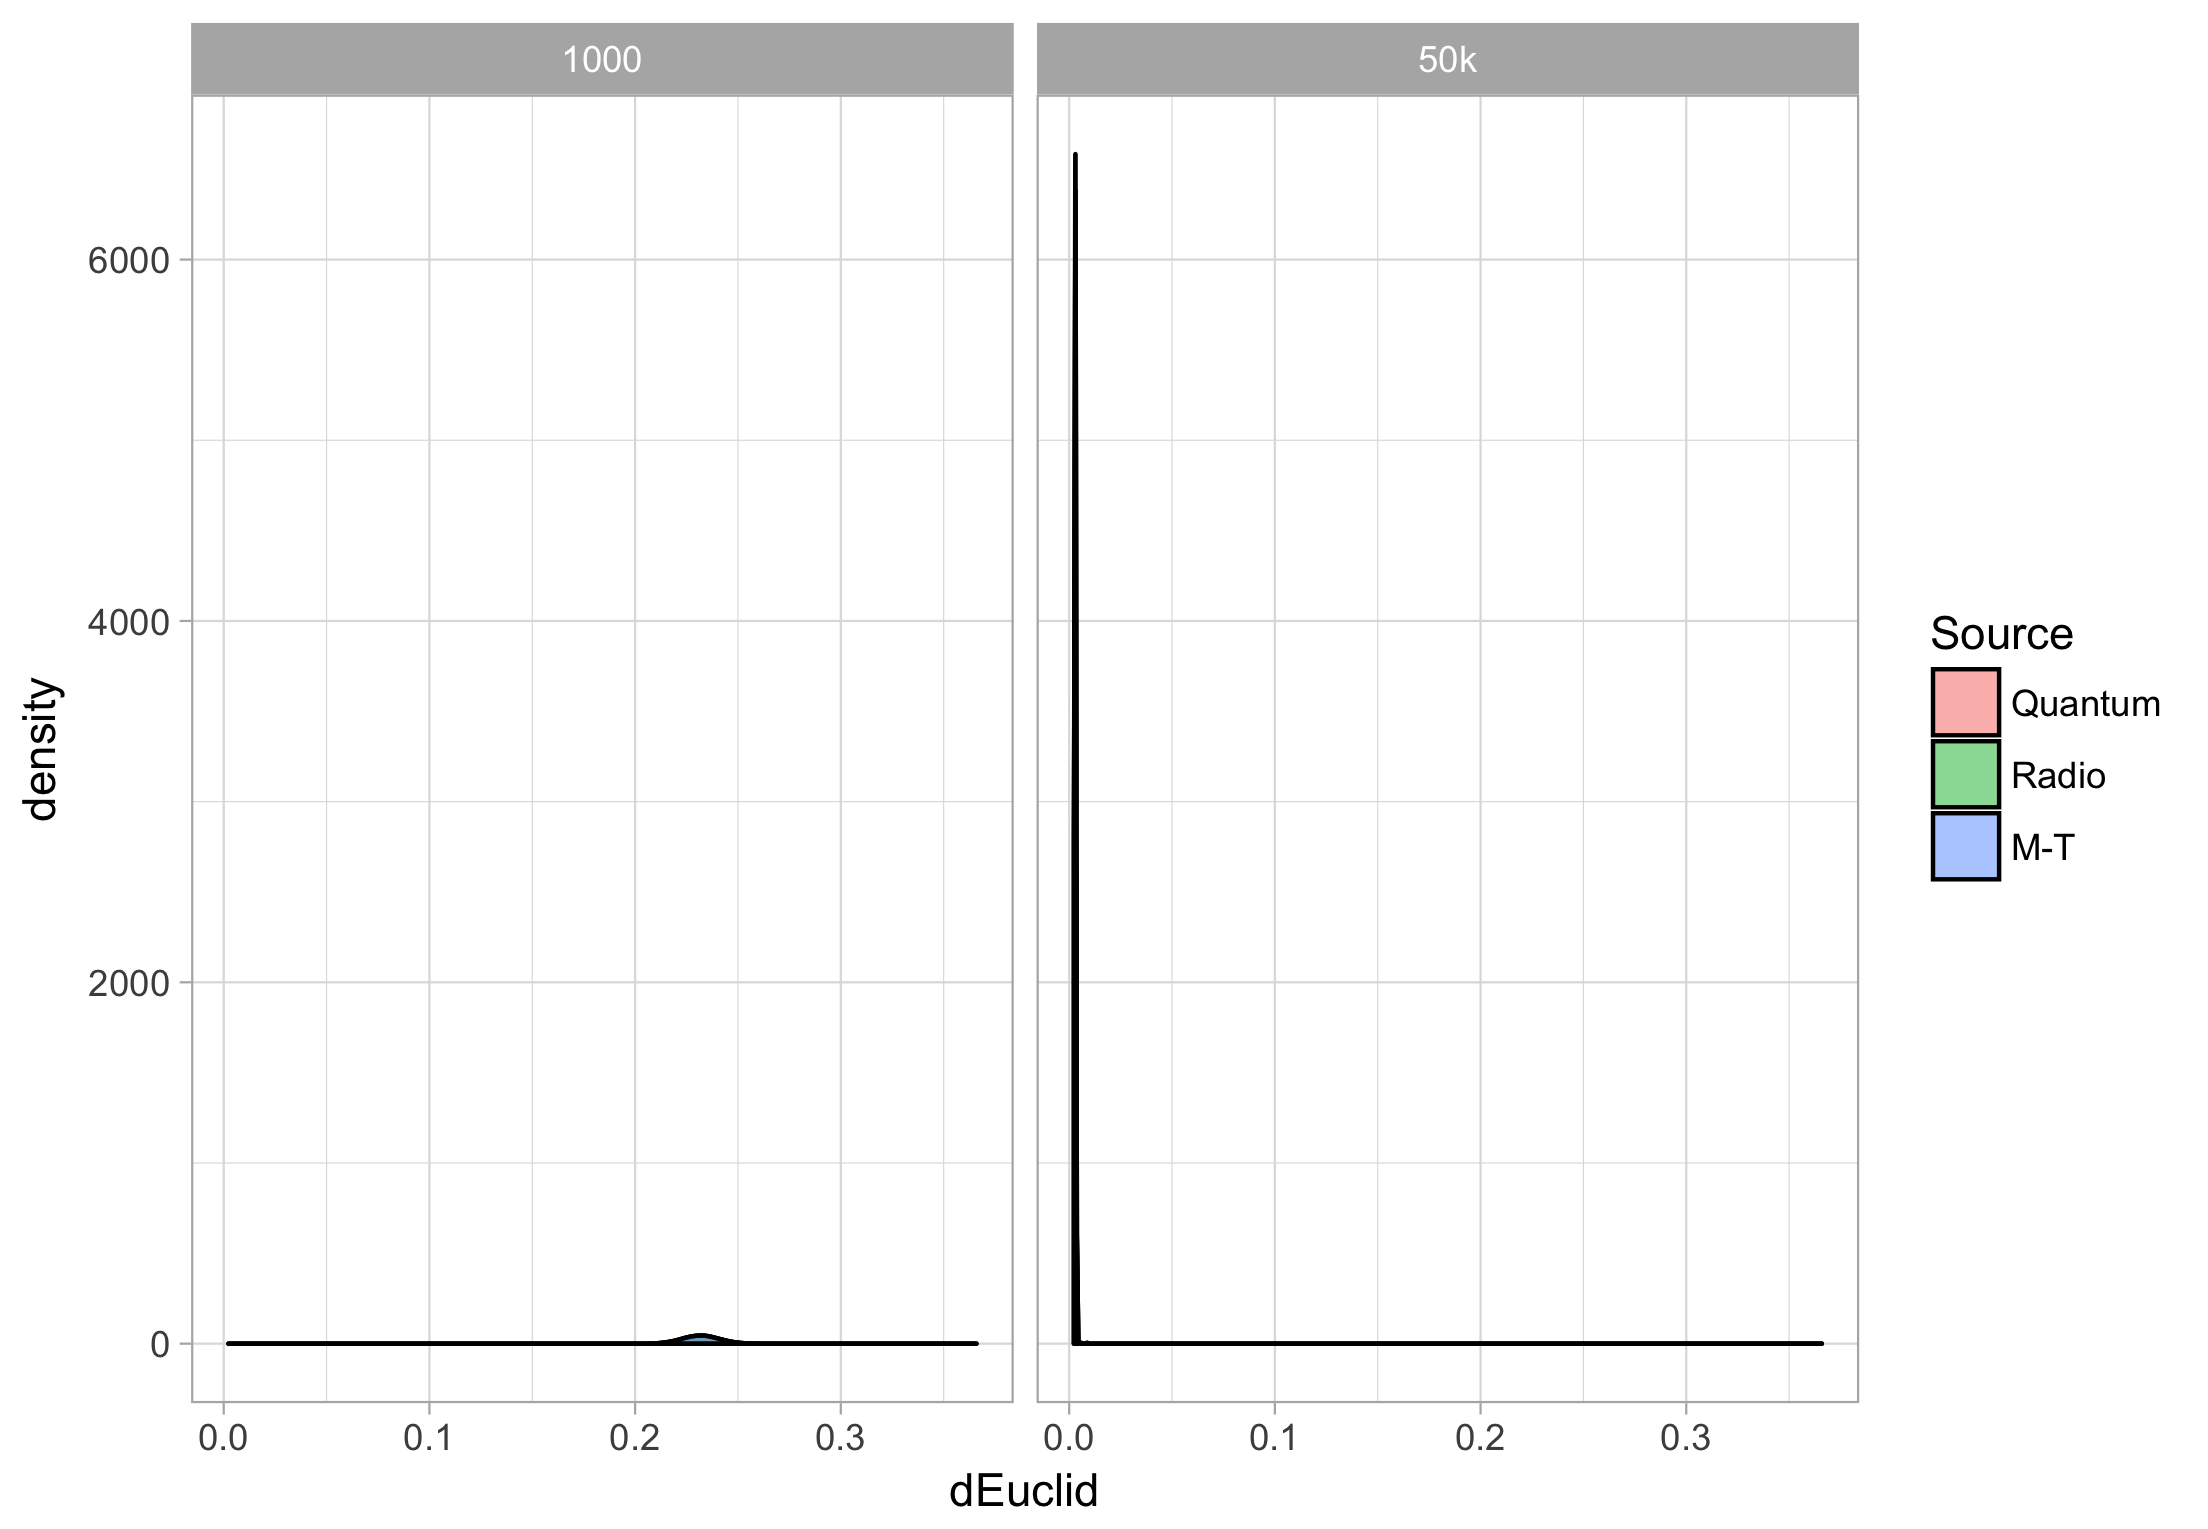
\includegraphics[width=.48\linewidth]{Hist_D6_t50}}
	\caption{Histogramas suavizados de situações que sugerem que o $N$ é um fator relevante}\label{fig:NRelevante}
\end{figure}

A figura~\ref{fig:DRelevante} mostra os histogramas suavizados das distâncias dos três geradores para dois tamanhos de sequências ($N=1.000$, $50.000$) e dois valores de \textit{lag} ($\tau=1$, $50$), sobrepondo os resultados obtidos com os diferentes tamanhos de palavras ($D=3$, $4$, $5$, $6$).
Os gráficos sugerem fortemente que o tamanho das palavras é um fator relevante para a distribuição da distância.

\begin{figure} %t 1 N 1000, D 3 D 4 D 5 D 6 %t 50 N 50000, D 3 D 4 D 5 D 6
	\centering
		\subfigure[$\tau=1$, $D=1.000$]{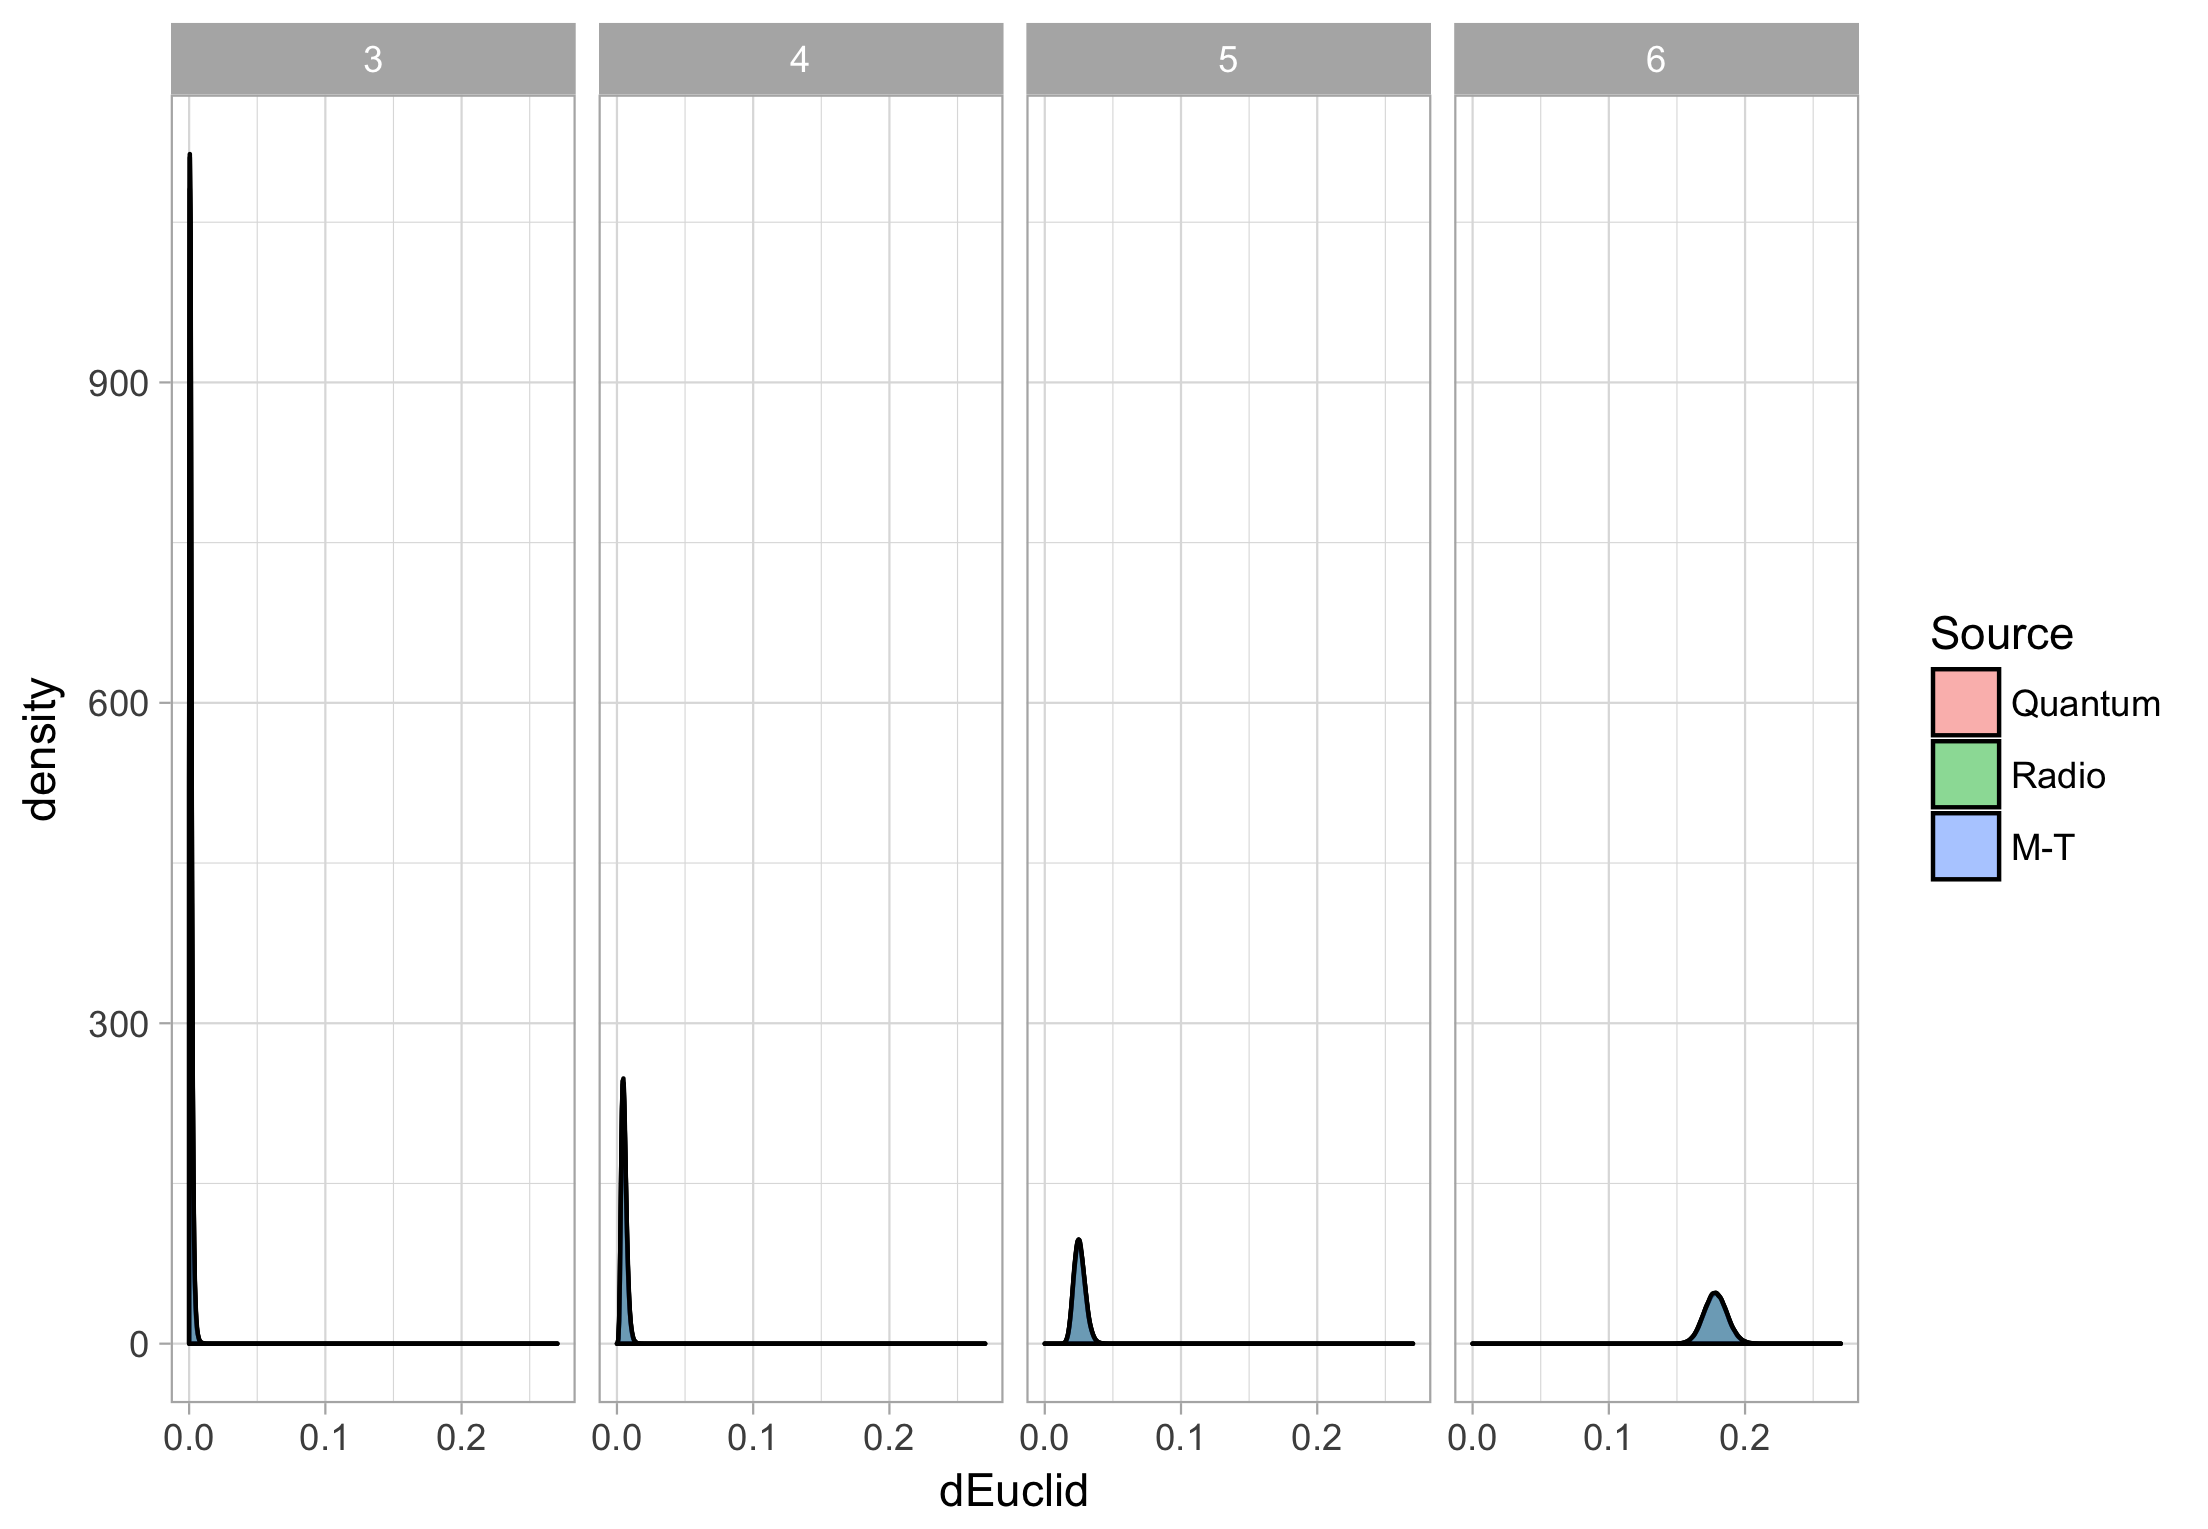
\includegraphics[width=.48\linewidth]{Hist_t1_1k}}
		\subfigure[$D=6$, $\tau=50$]{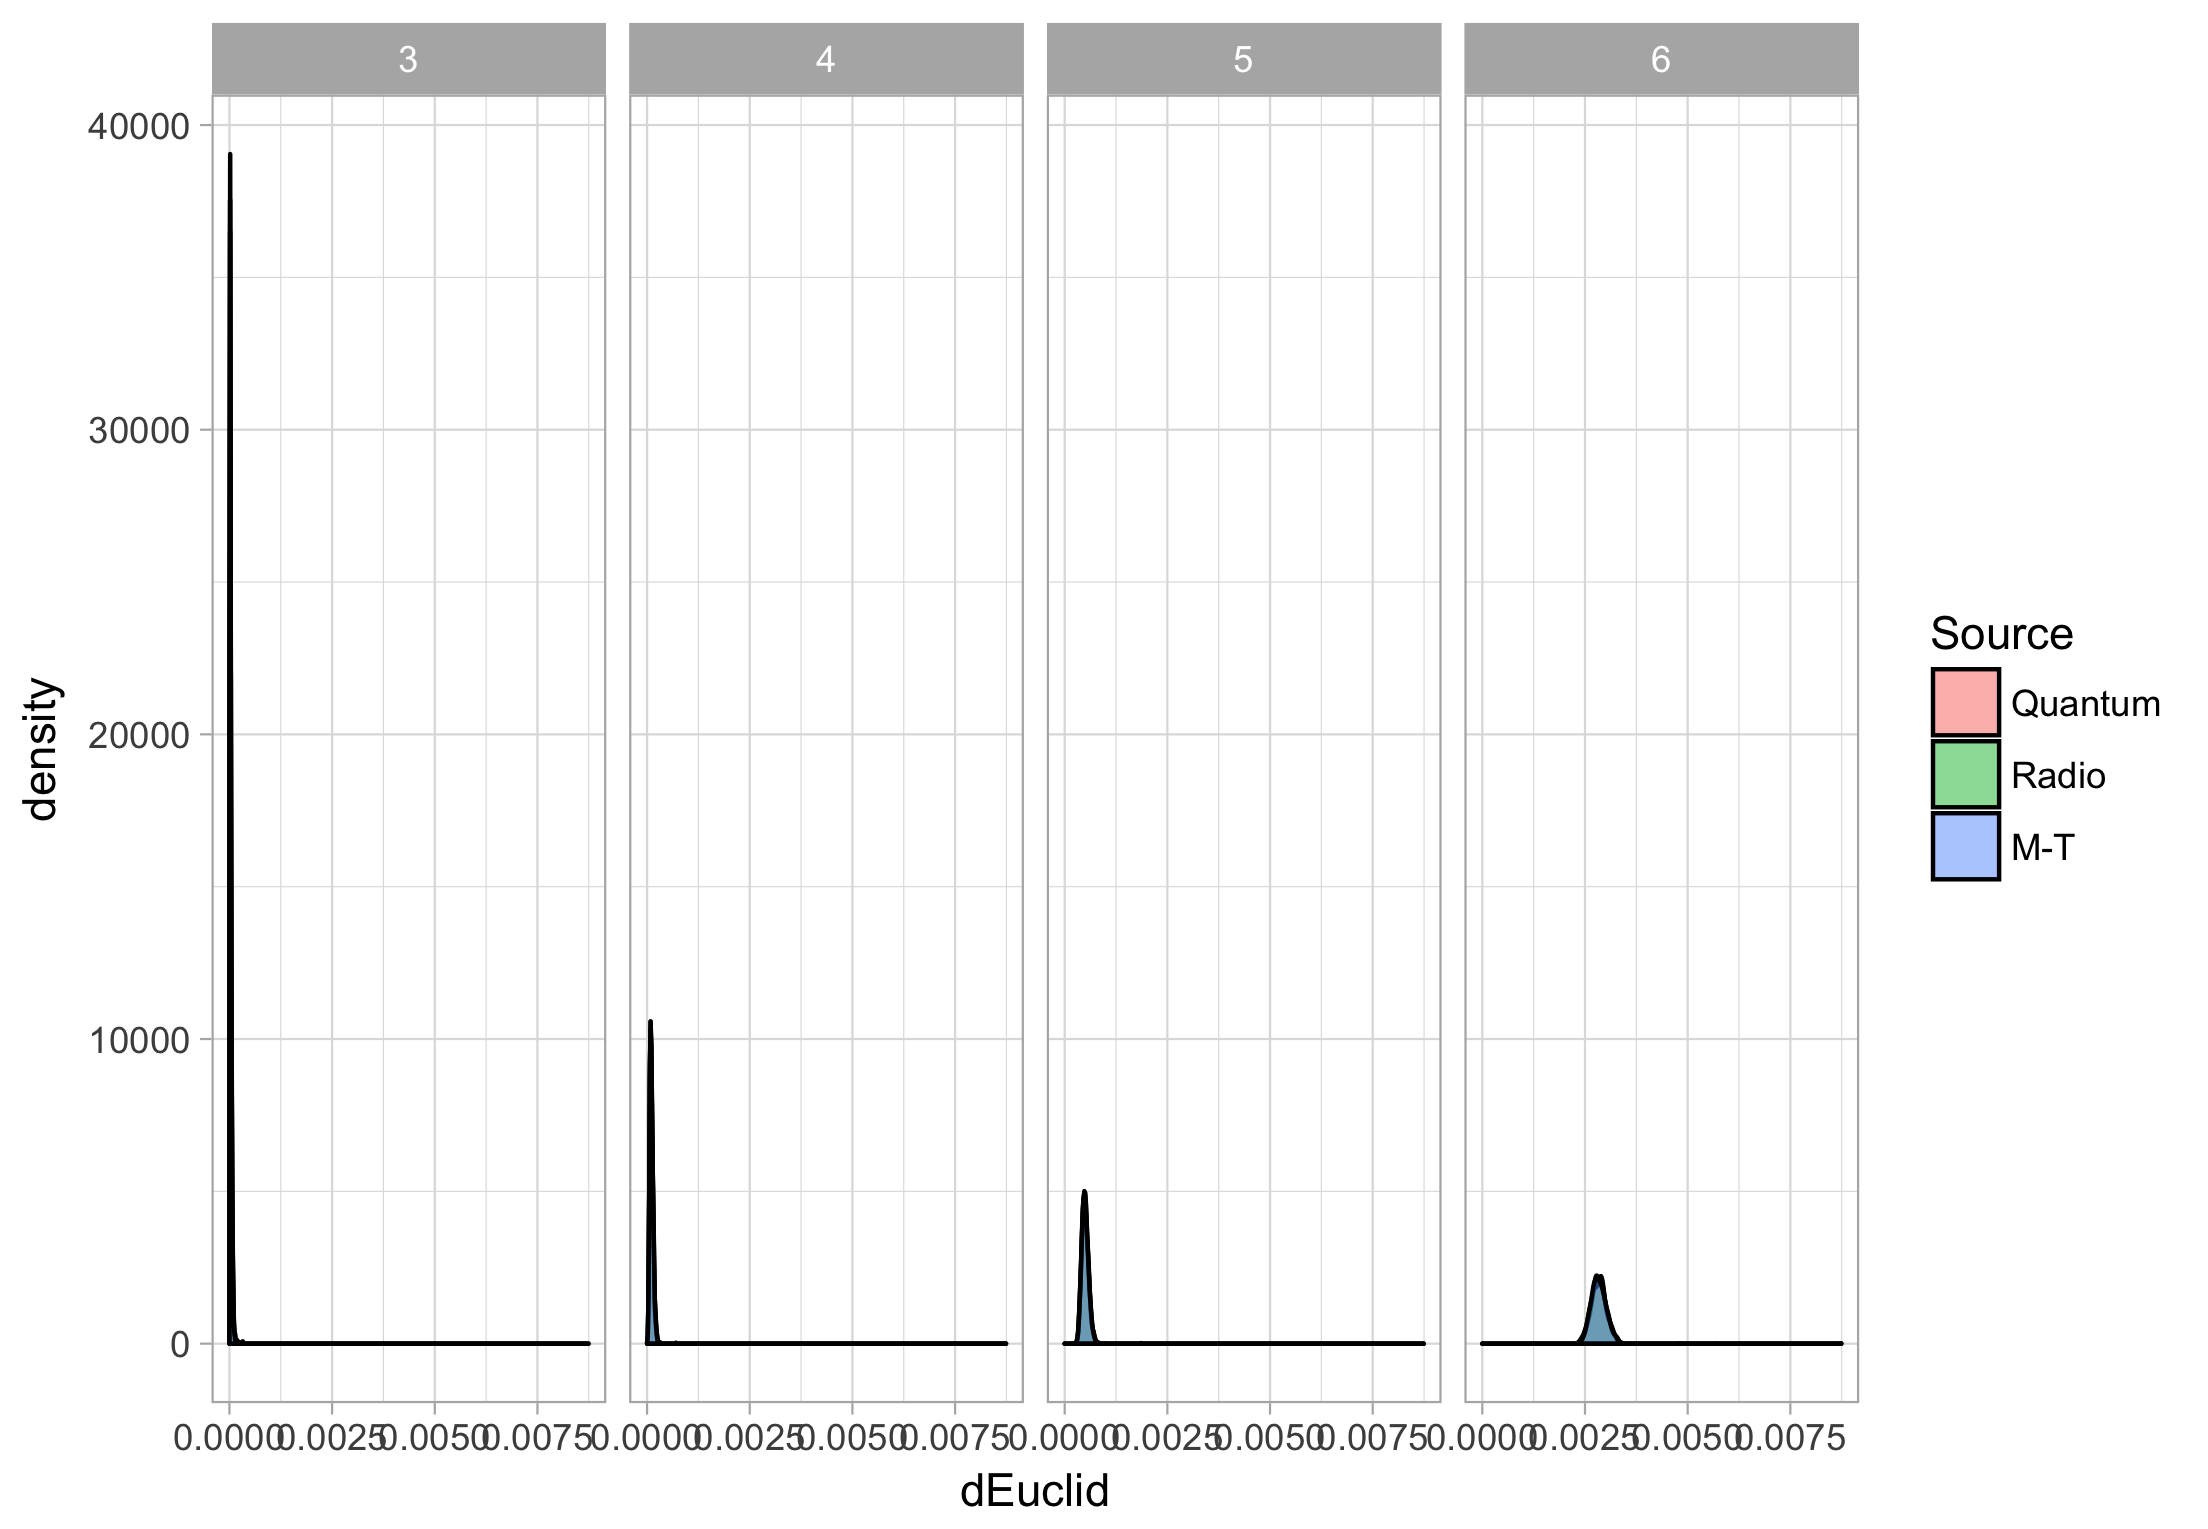
\includegraphics[width=.48\linewidth]{Hist_t50_50k}}
	\caption{Histogramas suavizados de situações que sugerem que o $D$ é um fator relevante}\label{fig:DRelevante}
\end{figure}



\begin{figure} %D 6 %N 1000, t 1 t 10 t 30 t 50 %N 50000, t 1 t 10 t 30 t 50
	\centering
	\subfigure[$\tau=1$, $D=1.000$]{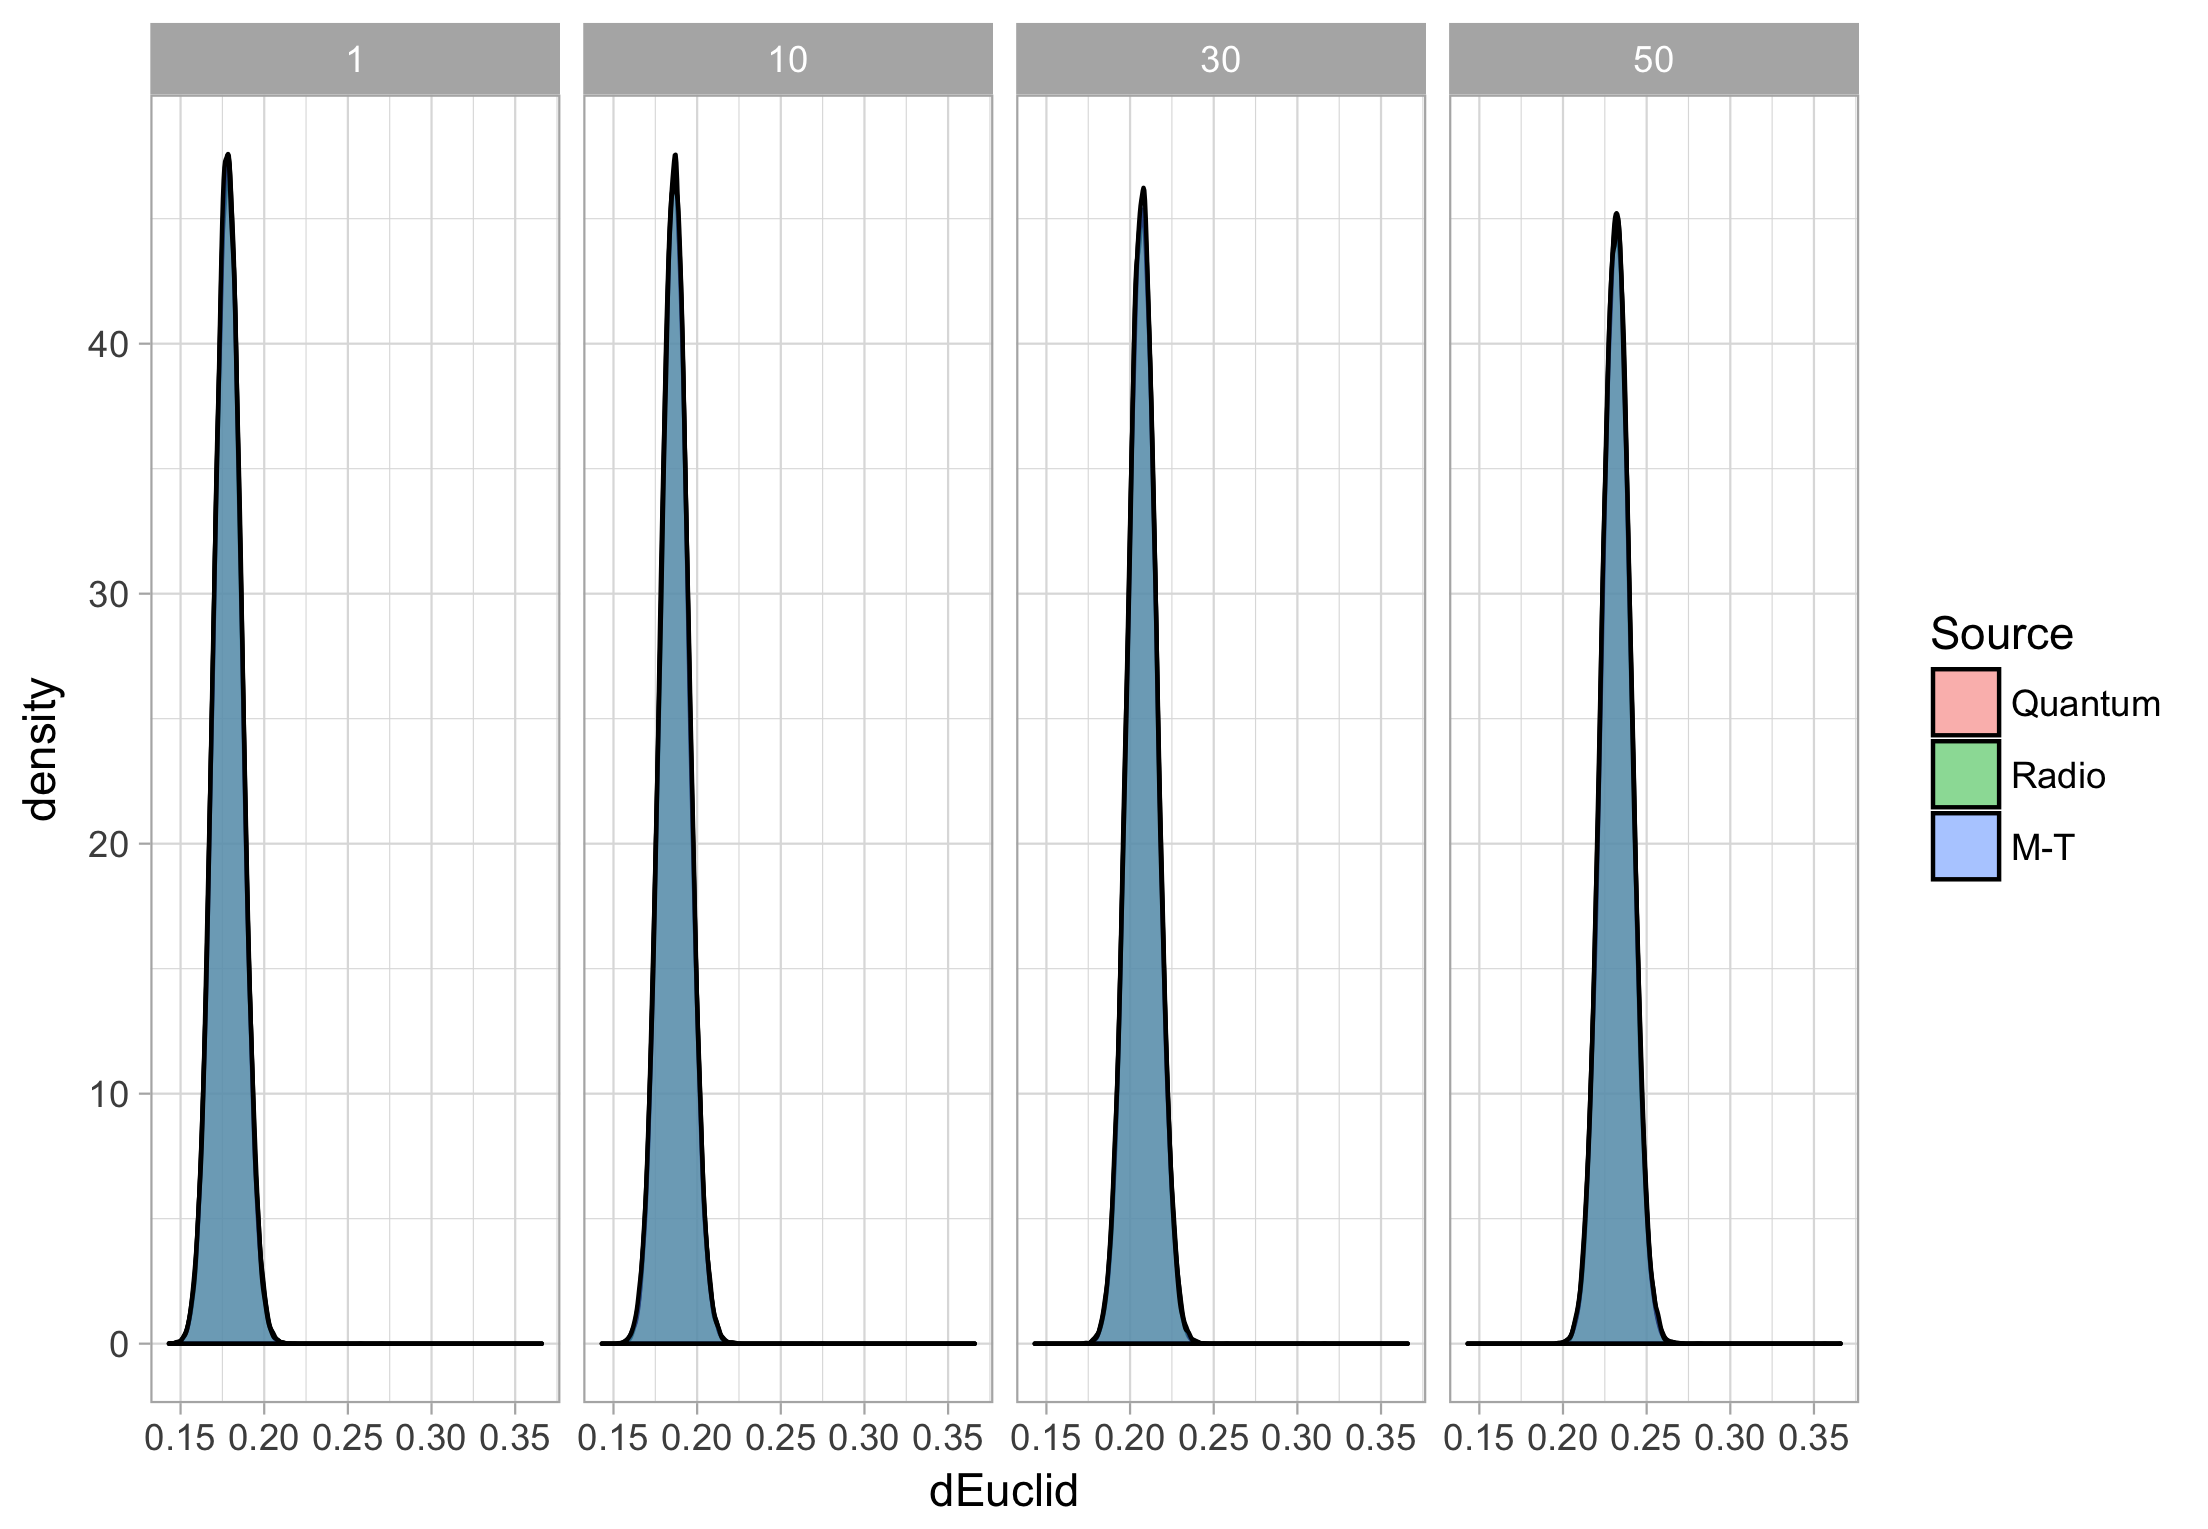
\includegraphics[width=.48\linewidth]{Hist_D6_1k}}
	\subfigure[$D=6$, $\tau=50$]{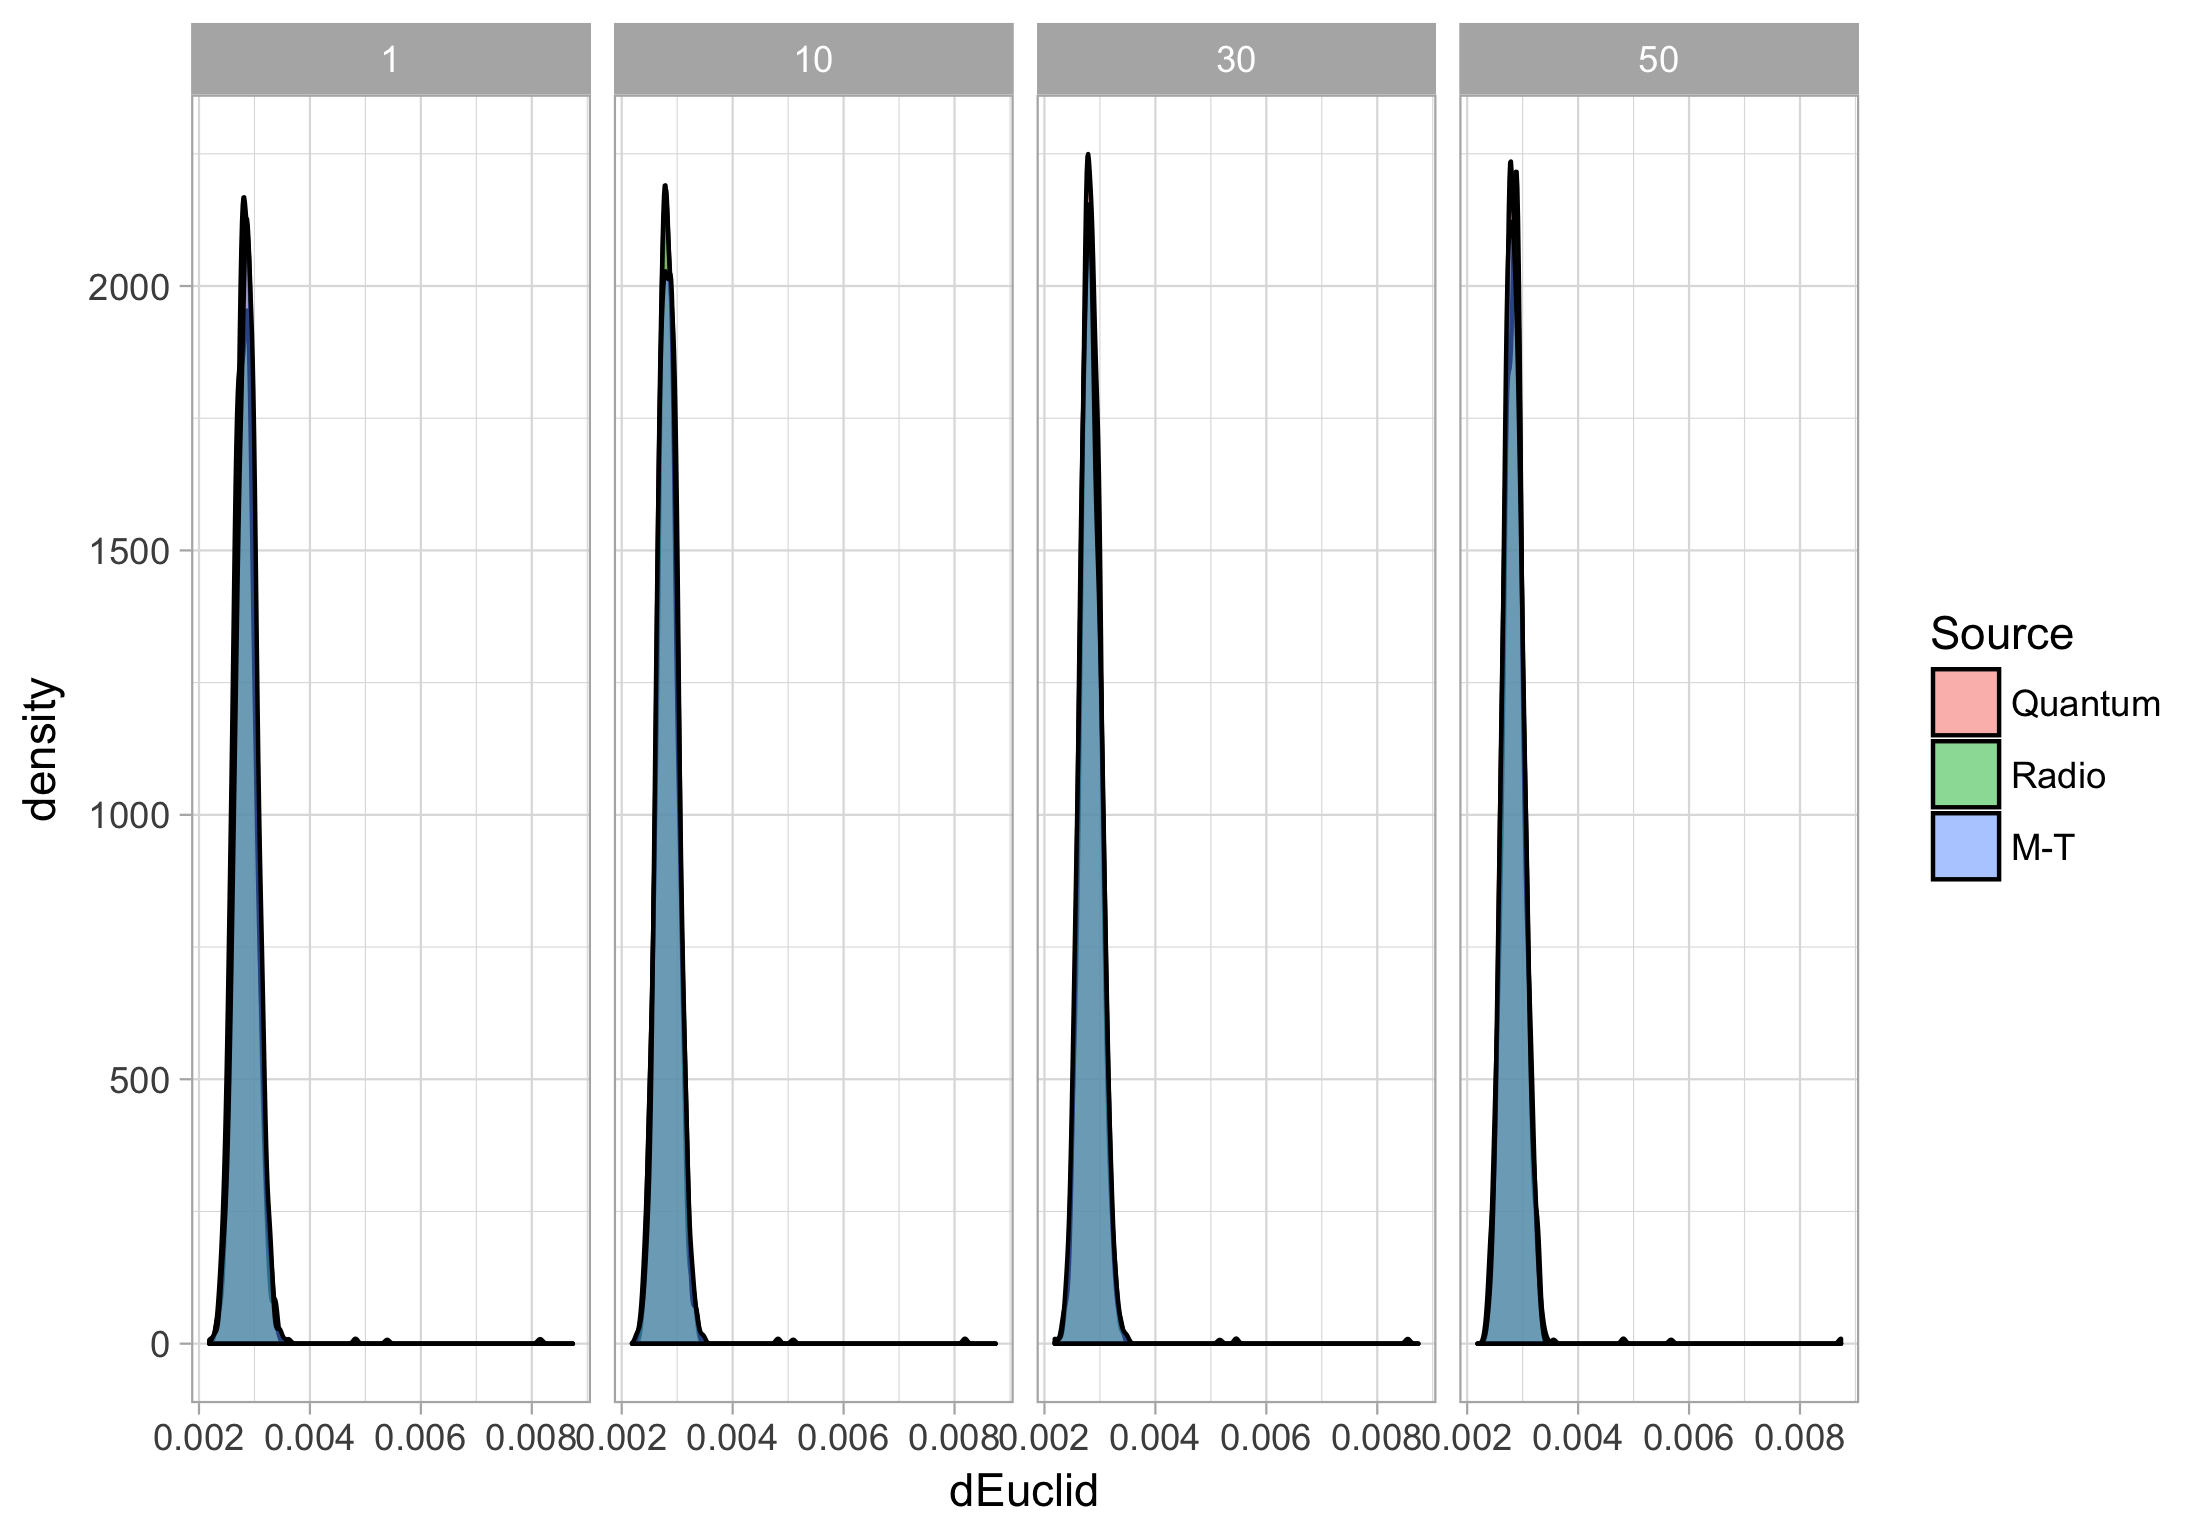
\includegraphics[width=.48\linewidth]{Hist_D6_50k}}
\caption{Histogramas suavizados de situações que sugerem que o $\tau$ é um fator relevante}\label{fig:tRelevante}
\end{figure}

Para consolidar esta análise realizamos a seguir testes Kolmogorov-Smirnov afim de analisar a influência dos fatores envolvidos nesta análise.

A Tabela~\ref{tab:KS_1000} mostra os $p$-valores dos testes de Kolmogorov-Smirnov aplicados a pares de distâncias calculadas sobre sequências de tamanho $1000$, variando $D$ e $\tau$.
Verificamos que há excelente aderência entre os pares de distâncias de sequências Quânticas e de Rádio.
Já quando a comparação é feita com distâncias de sequências de Mersenne-Twister (M-T), a aderência diminui um pouco.

\begin{table}[hbt]
	\centering
	\caption{Teste de Kolmogorov-Smirnov aplicado a pares de sequências para $1.000$ observações.}\label{tab:KS_1000}
	\begin{tabular}{cccccc}
		\toprule
		Par  &    $D$ & $\tau=1$   &   $\tau=10$   &   $\tau=30$   &   $\tau=50$   \\ \midrule
Quântica vs.\ Rádio		& $D=3$ & 0.18034676 & 0.08582490 & 0.58096350 & 0.32626542 \\
		& $D=4$ & 0.21708776 & 0.60690204 & 0.08116764 & 0.46372312  \\
		& $D=5$ & 0.32388371 & 0.53394280 & 0.46970138 & 0.02768674  \\
		& $D=6$ & 0.61501858 & 0.63403661 & 0.54795745 & 0.15353799  \\ \midrule
Quântica vs. M-T & $D=3$ & 0.09400120 & 0.22995096 & 0.36766759 &  0.03706359 \\
		& $D=4$ & 0.25188769 & 0.35844686 & 0.16768952 &  0.18237754 \\
		& $D=5$ & 0.97552039 & 0.79878301 & 0.12852918 &  0.08764347 \\
		& $D=6$ & 0.47615384 & 0.42420007 & 0.55290011 &  0.79669144 \\ \midrule
Rádio vs.\ M-T & $D=3$ & 0.008560614 & 0.496450214 & 0.982419336 & 0.390237891 \\
		& $D=4$ & 0.003804157 & 0.229503619 & 0.629158543 & 0.651783589 \\
		& $D=5$ & 0.254216237 & 0.179697451 & 0.824743440 & 0.071709252 \\
		& $D=6$ & 0.846441994 & 0.033726860 & 0.493286733 & 0.184856861 \\
		\bottomrule
	\end{tabular}
\end{table}

Os $p$-valores reportados para distâncias obtidas com sequências de tamanho $N=1000$ não permitem concluir que haja diferenças significativas.
Essa constatação será revertida ao analisar distâncias entre sequências de tamanho $N=50000$.

A Tabela~\ref{tab:KS_50k} mostra os $p$-valores dos testes de Kolmogorov-Smirnov aplicados a pares de distâncias calculadas sobre sequências de tamanho $50000$, variando $D$ e $\tau$.
Verificamos que há excelente aderência entre os pares de distâncias de sequências Quânticas e de Rádio.
Já quando a comparação é feita com distâncias de sequências de Mersenne-Twister (M-T), a aderência diminui de forma sistemática e significativa para $\tau=1$.

\begin{table}[hbt]
	\centering
	\caption{Teste de Kolmogorov-Smirnov aplicado a pares de sequências para $50.000$ observações.}\label{tab:KS_50k}
	\begin{tabular}{cccccc}
		\toprule
		Par  & $D$ &   $\tau=1$   &   $\tau=10$   &   $\tau=30$   &   $\tau=50$   \\ \midrule
Quântica vs.\ Rádio		& $D=3$ & 0.13862662 & 0.93677447 & 0.07714702 &  0.46405291 \\
		& $D=4$ & 0.68079537 & 0.90035466 & 0.60801914 &  0.77908261 \\
		& $D=5$ & 0.14371256 & 0.76662067 & 0.64456996 &  0.91315843 \\
		& $D=6$ & 0.02268670 & 0.49307044 & 0.53135926 &  0.30074267 \\ \midrule
Quântica vs.\ M-T & $D=3$ & 6.074571e-10 & 1.388898e-01 & 2.682058e-01 & 4.822849e-01 \\
		& $D=4$ & 6.592620e-09 & 2.987721e-02 & 8.438134e-01 & 7.923220e-01 \\
		& $D=5$ & 9.424114e-08 & 3.289299e-02 & 7.681676e-01 & 8.405168e-01 \\
		& $D=6$ & 9.058821e-04 & 7.075225e-01 & 2.982731e-01 & 3.614763e-01 \\ \midrule
Rádio vs.\ M-T		& $D=3$ & 1.226271e-09 & 1.609665e-01 & 1.465970e-01 & 1.914937e-01 \\
		& $D=4$ & 2.190462e-10 & 1.277762e-02 & 2.069821e-01 & 9.963221e-01 \\
		& $D=5$ & 1.438372e-11 & 1.267622e-02 & 4.364935e-01 & 9.999998e-01 \\
		& $D=6$ & 3.749001e-06 & 2.263466e-01 & 7.419248e-01 & 4.014641e-01 \\
		\bottomrule
	\end{tabular}
\end{table}

Os $p$-valores observados na Tabela~\ref{tab:KS_50k} nos levam a concluir que não é possível desconsiderar a fonte de dados como um fator relevante quando se trata do gerador de Mersenne-Twister.
Já as distâncias das sequências produzidas pelos geradores Quântico e de Rádio são indistinguíveis e, portanto, não podemos descartar a hipótese dessas fontes serem idênticas para a medida considerada.

%A figura~\ref{Fig:ScatterAllRandom} mostra os planos Entropia-Complexidade com as respectivas curvas de complexidade mínima e máxima para cada par $D\in\{3,4,5,6\}$ (colunas) e $\tau\in\{1,10,30,50\}$ (linhas), com os \num{52429} pontos observados a partir das sequências obtidas pelo gerador de rádio.
%Os pontos foram desenhados com \SI{1}{\percent} de transparência, para evidenciar as regiões mais e menos densas.
%
%\begin{figure}[hbt]
%	\centering
%	\includegraphics[width=\linewidth]{ScatterAllRandom}
%	\caption{Diagramas de dispersão das sequências de rádio para $D\in\{3,4,5,6\}$ (colunas) e $\tau\in\{1,10,30,50\}$ (linhas), com curvas de complexidade mínima e máxima no plano Entropia-Complexidade.}\label{Fig:ScatterAllRandom}
%\end{figure}
%
%A figura~\ref{Fig:ScatterAllMT} mostra os planos Entropia-Complexidade com as respectivas curvas de complexidade mínima e máxima para cada par $D\in\{3,4,5,6\}$ (colunas) e $\tau\in\{1,10,30,50\}$ (linhas), com os \num{52429} pontos observados a partir das sequências obtidas pelo gerador de Mersenne-Twister.
%Os pontos foram desenhados com \SI{1}{\percent} de transparência, para evidenciar as regiões mais e menos densas.
%
%\begin{figure}[hbt]
%	\centering
%	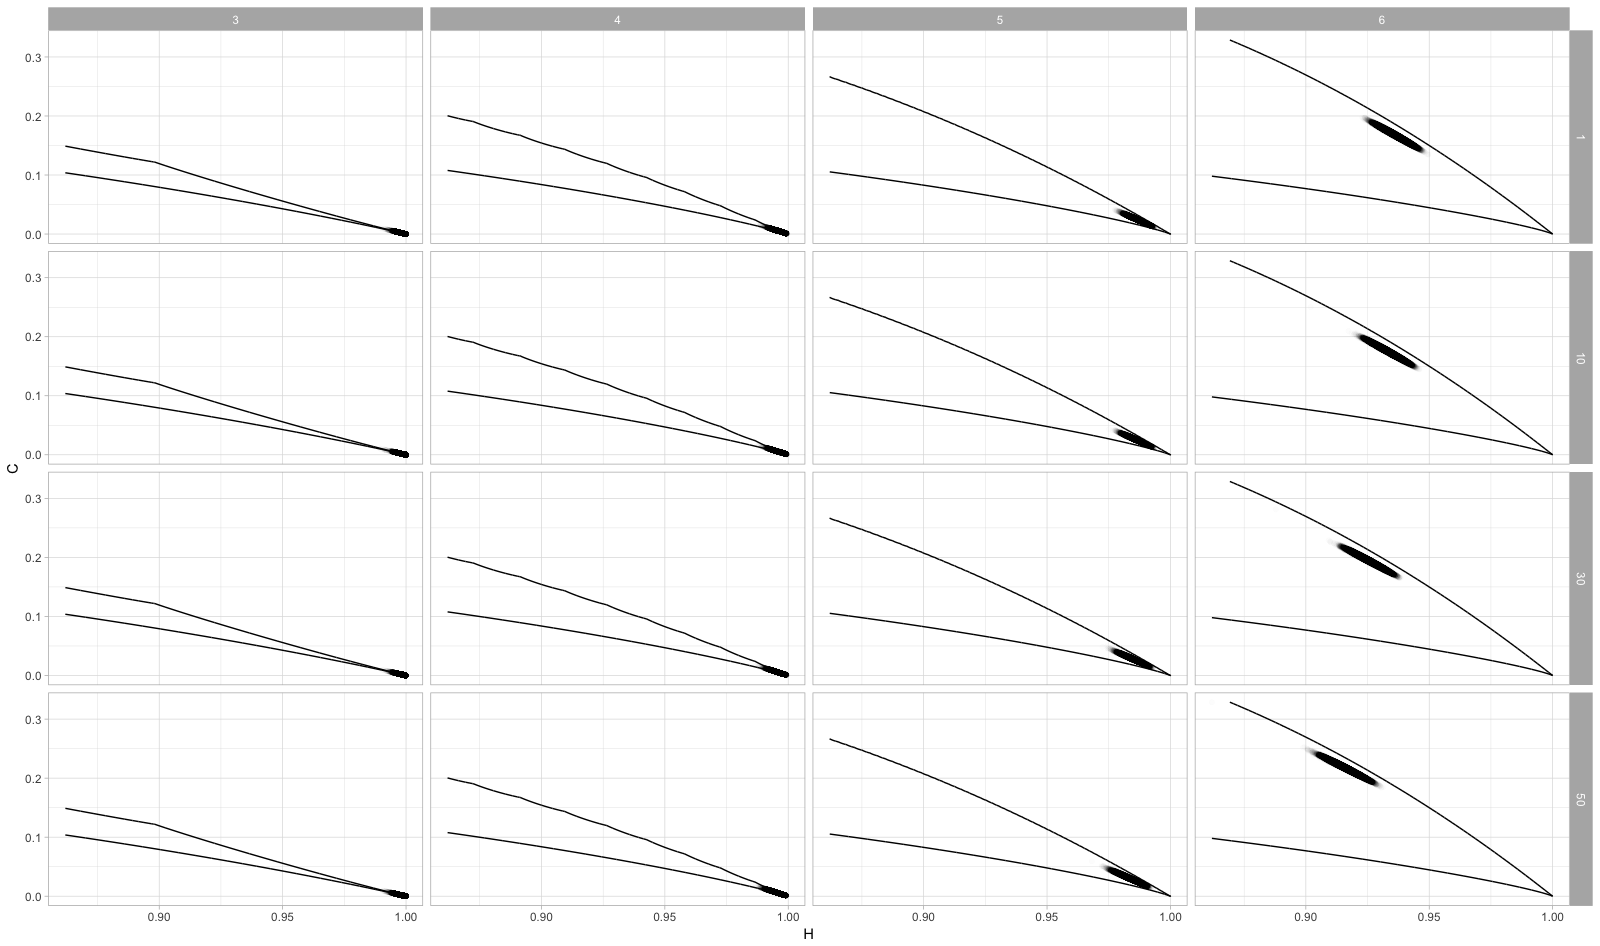
\includegraphics[width=\linewidth]{ScatterAllMT}
%	\caption{Diagramas de dispersão das sequências de Mersenne-Twister para $D\in\{3,4,5,6\}$ (colunas) e $\tau\in\{1,10,30,50\}$ (linhas), com curvas de complexidade mínima e máxima no plano Entropia-Complexidade.}\label{Fig:ScatterAllMT}
%\end{figure}

\begin{figure}[hbt]
\centering
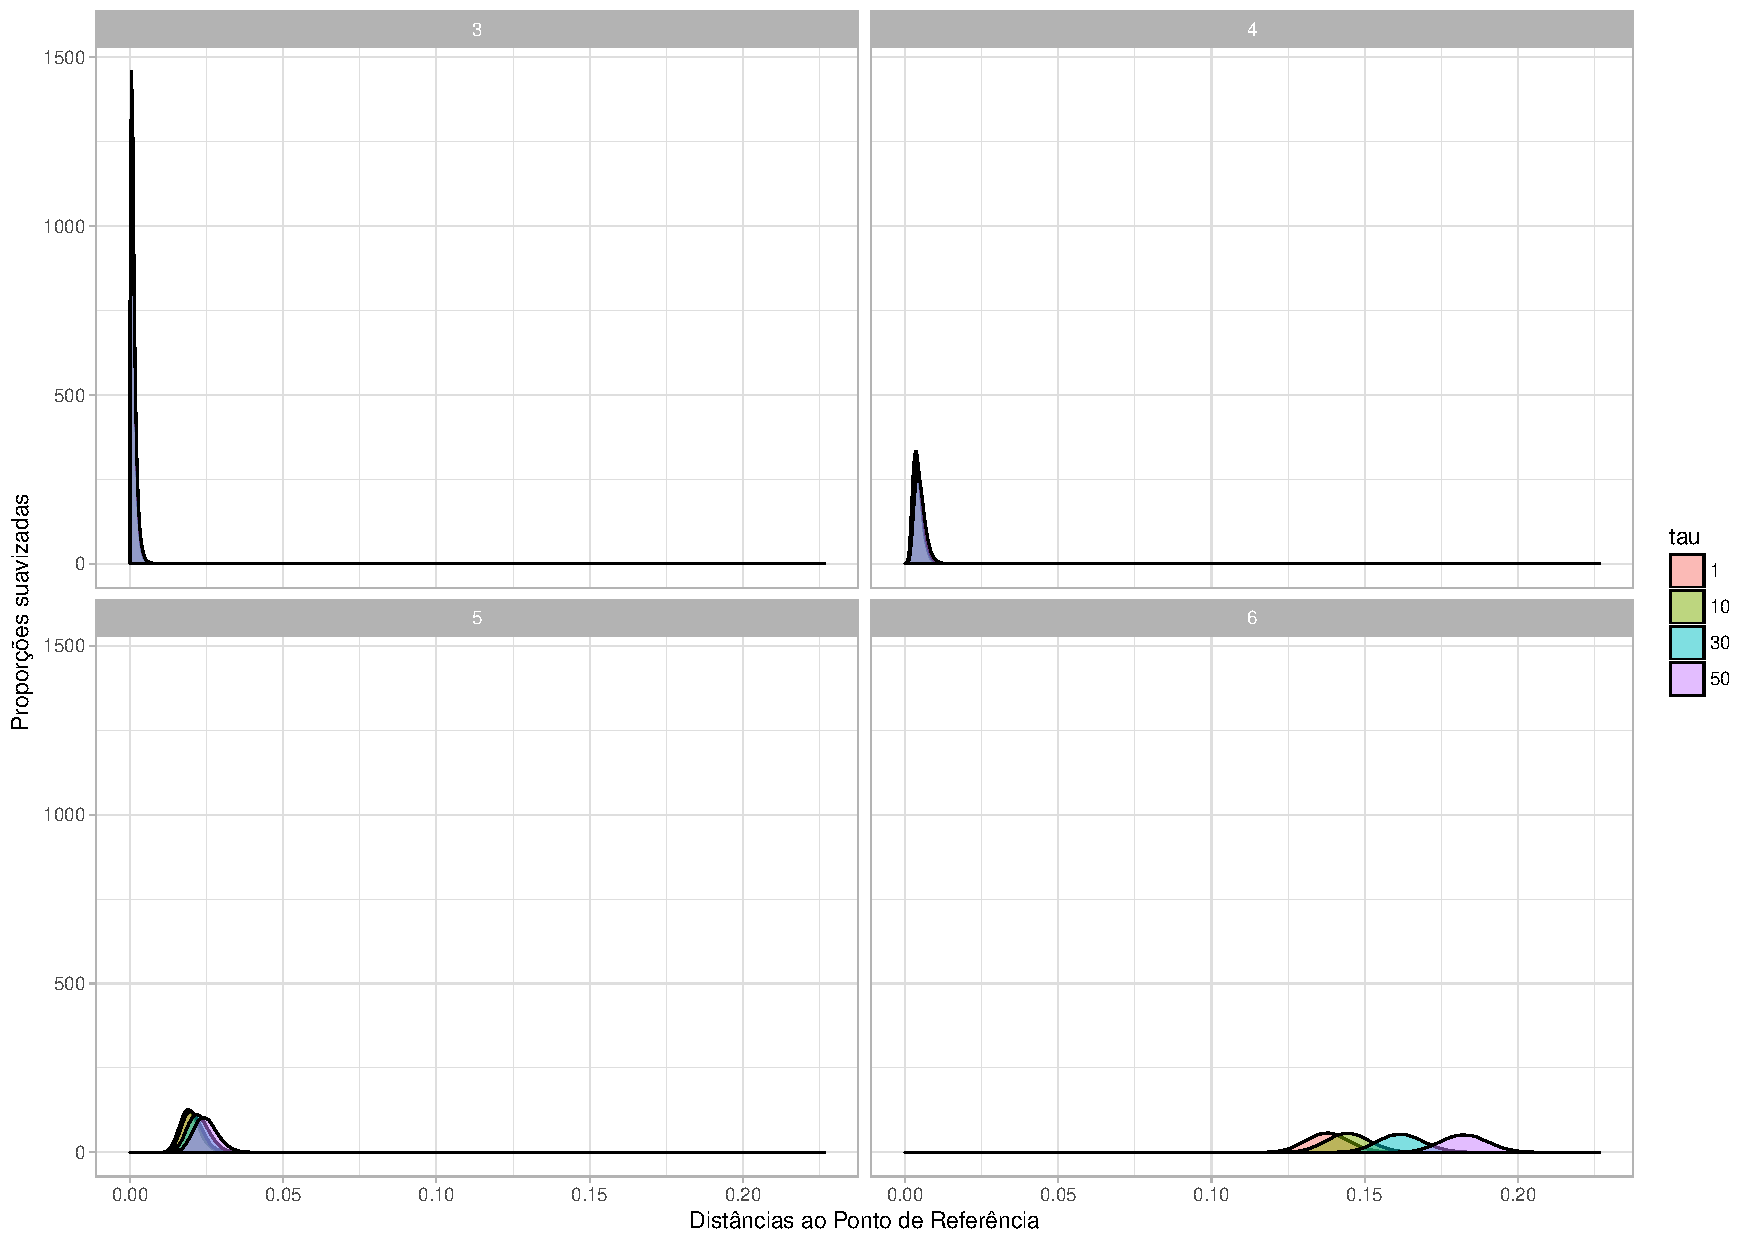
\includegraphics[width=\linewidth]{HistoDistanciasQuantTodas}
\caption{Histogramas suavizados das distâncias euclidianas dos padrões ao ponto de referência, para $D\in\{3,4,5,6\}$ (colunas) e $\tau\in\{1,10,30,50\}$ (linhas).}\label{Fig:HistoDistanciasQuantTodas}
\end{figure}

A figura~\ref{Fig:HistoDistanciasQuantTodas} sugere que o comportamento das distâncias euclidianas ao ponto de referência muda conforme o tamanho do padrão $D$ varia.
Além disso, também são perceptíveis mudanças de comportamento em função do \textit{lag} $\tau$ quando $D=5,6$.

Da análise aqui apresentada concluímos que, à luz da distância do ponto característico de uma sequência ao ponto de referência, os dois geradores físicos produzem sequências indistinguíveis.
Diante disso, nos cálculos subsequentes faremos a junção desses conjuntos de dados, que denominaremos simplesmente ``aleatórios'' no que segue.

Já o gerador de Mersenne-Twister apresenta diferenças em relação aos geradores de origem física.
Por se tratar de um gerador algorítmico e, portanto, pseudoaleatório, ele será tratado como objeto de análise e não como padrão para estabelecer critérios de qualidade.

\section{Análise das sequências aleatórias}

\begin{figure}
\centering
\subfigure[Escala linear\label{Fig:scatter1000D3t1}]{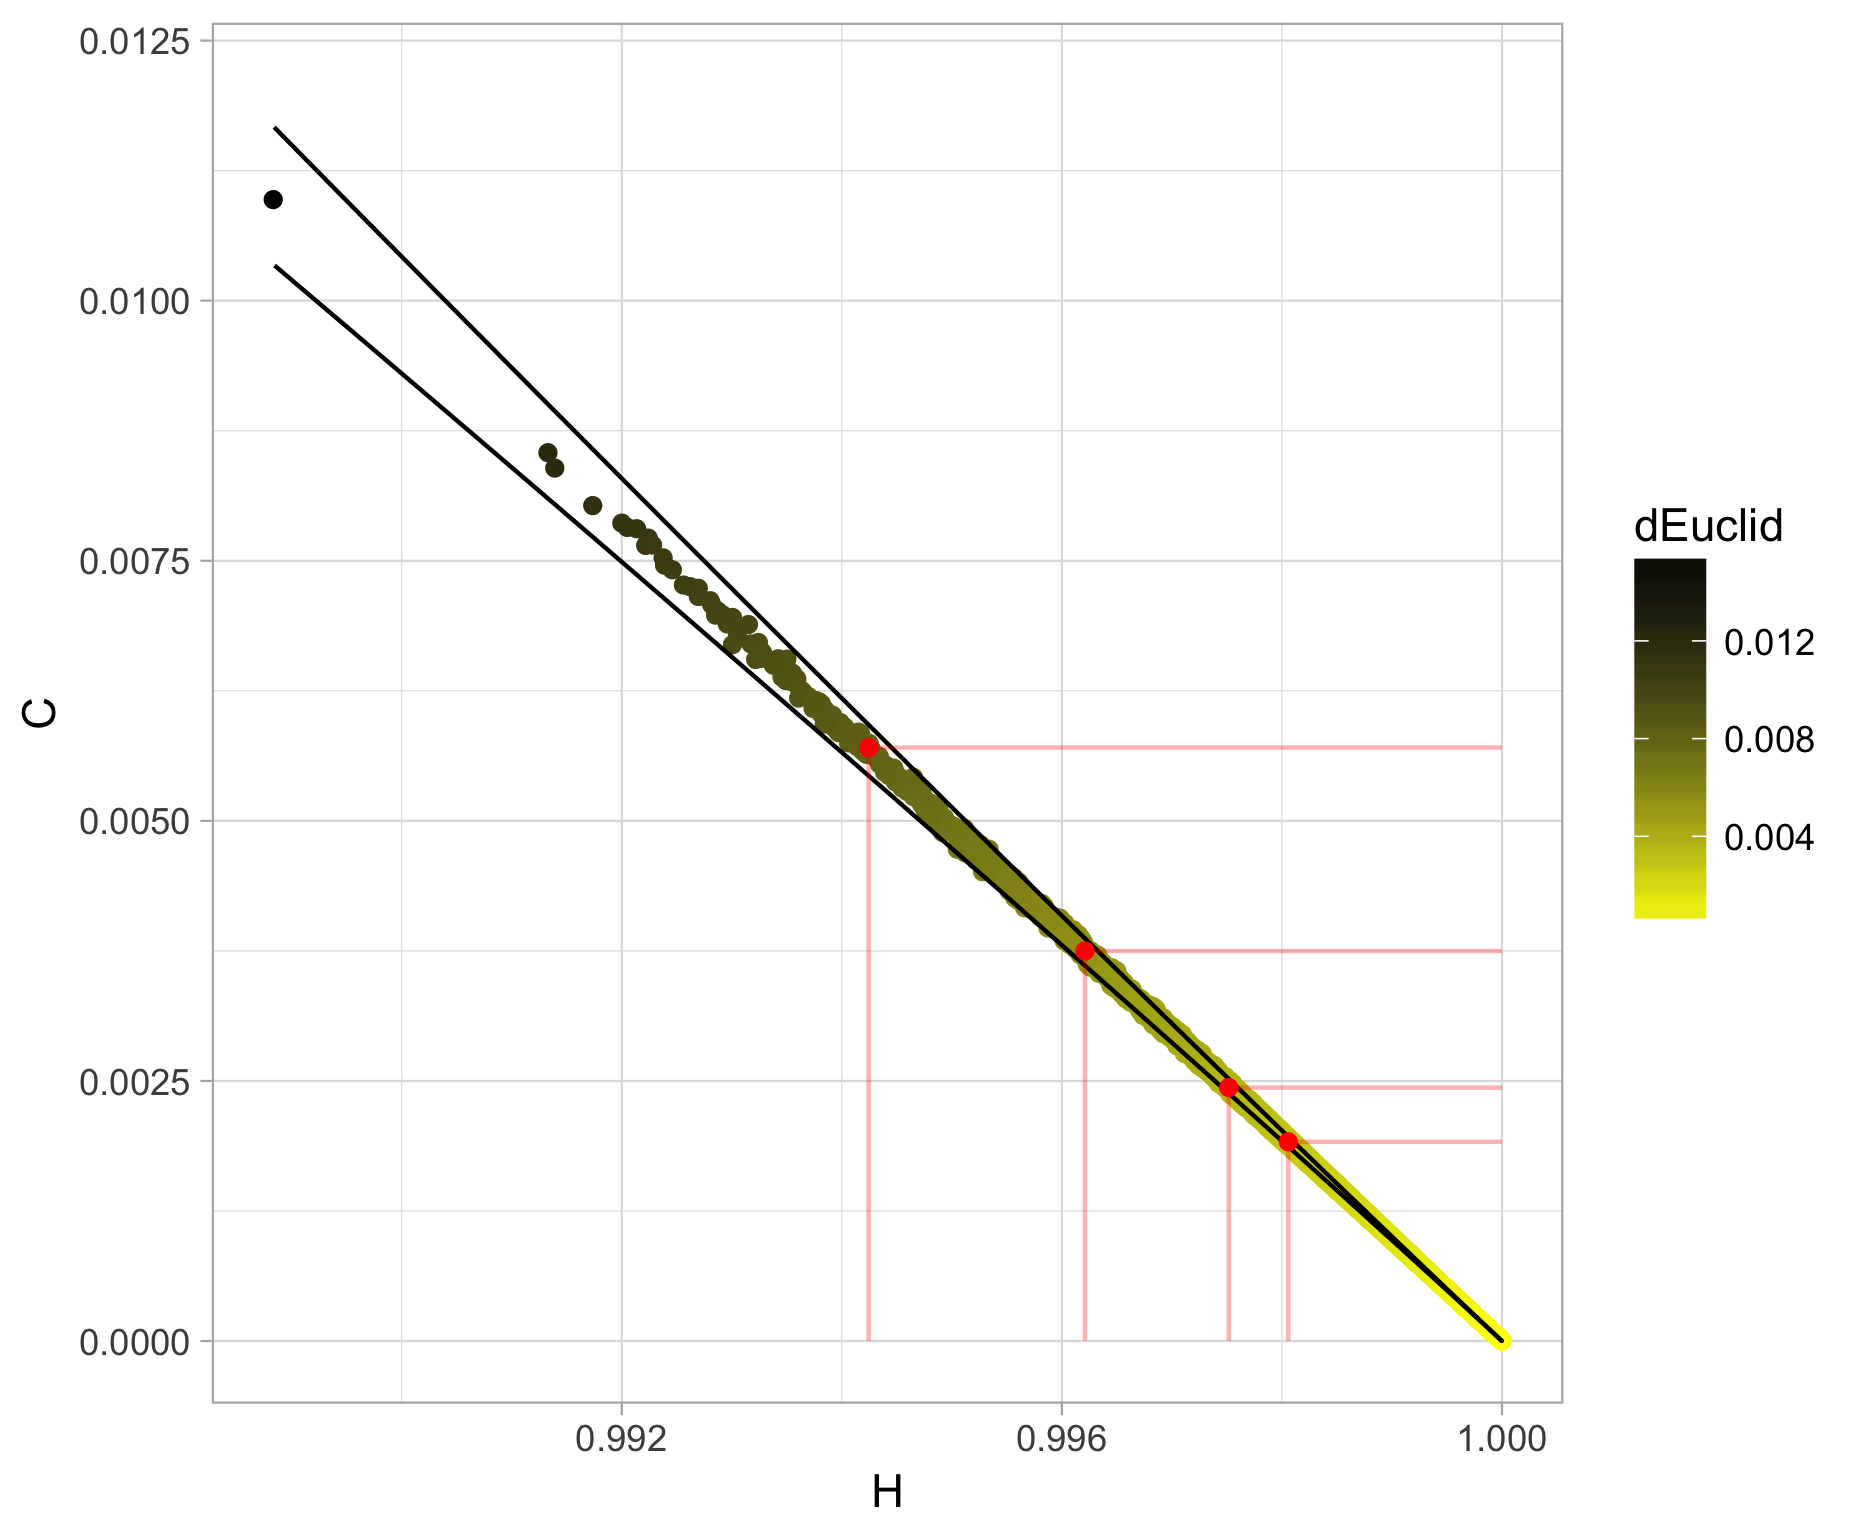
\includegraphics[width=.48\linewidth]{scatter1000D3t1}}
\subfigure[Escala logarítmica\label{Fig:scatter1000D3t1_log}]{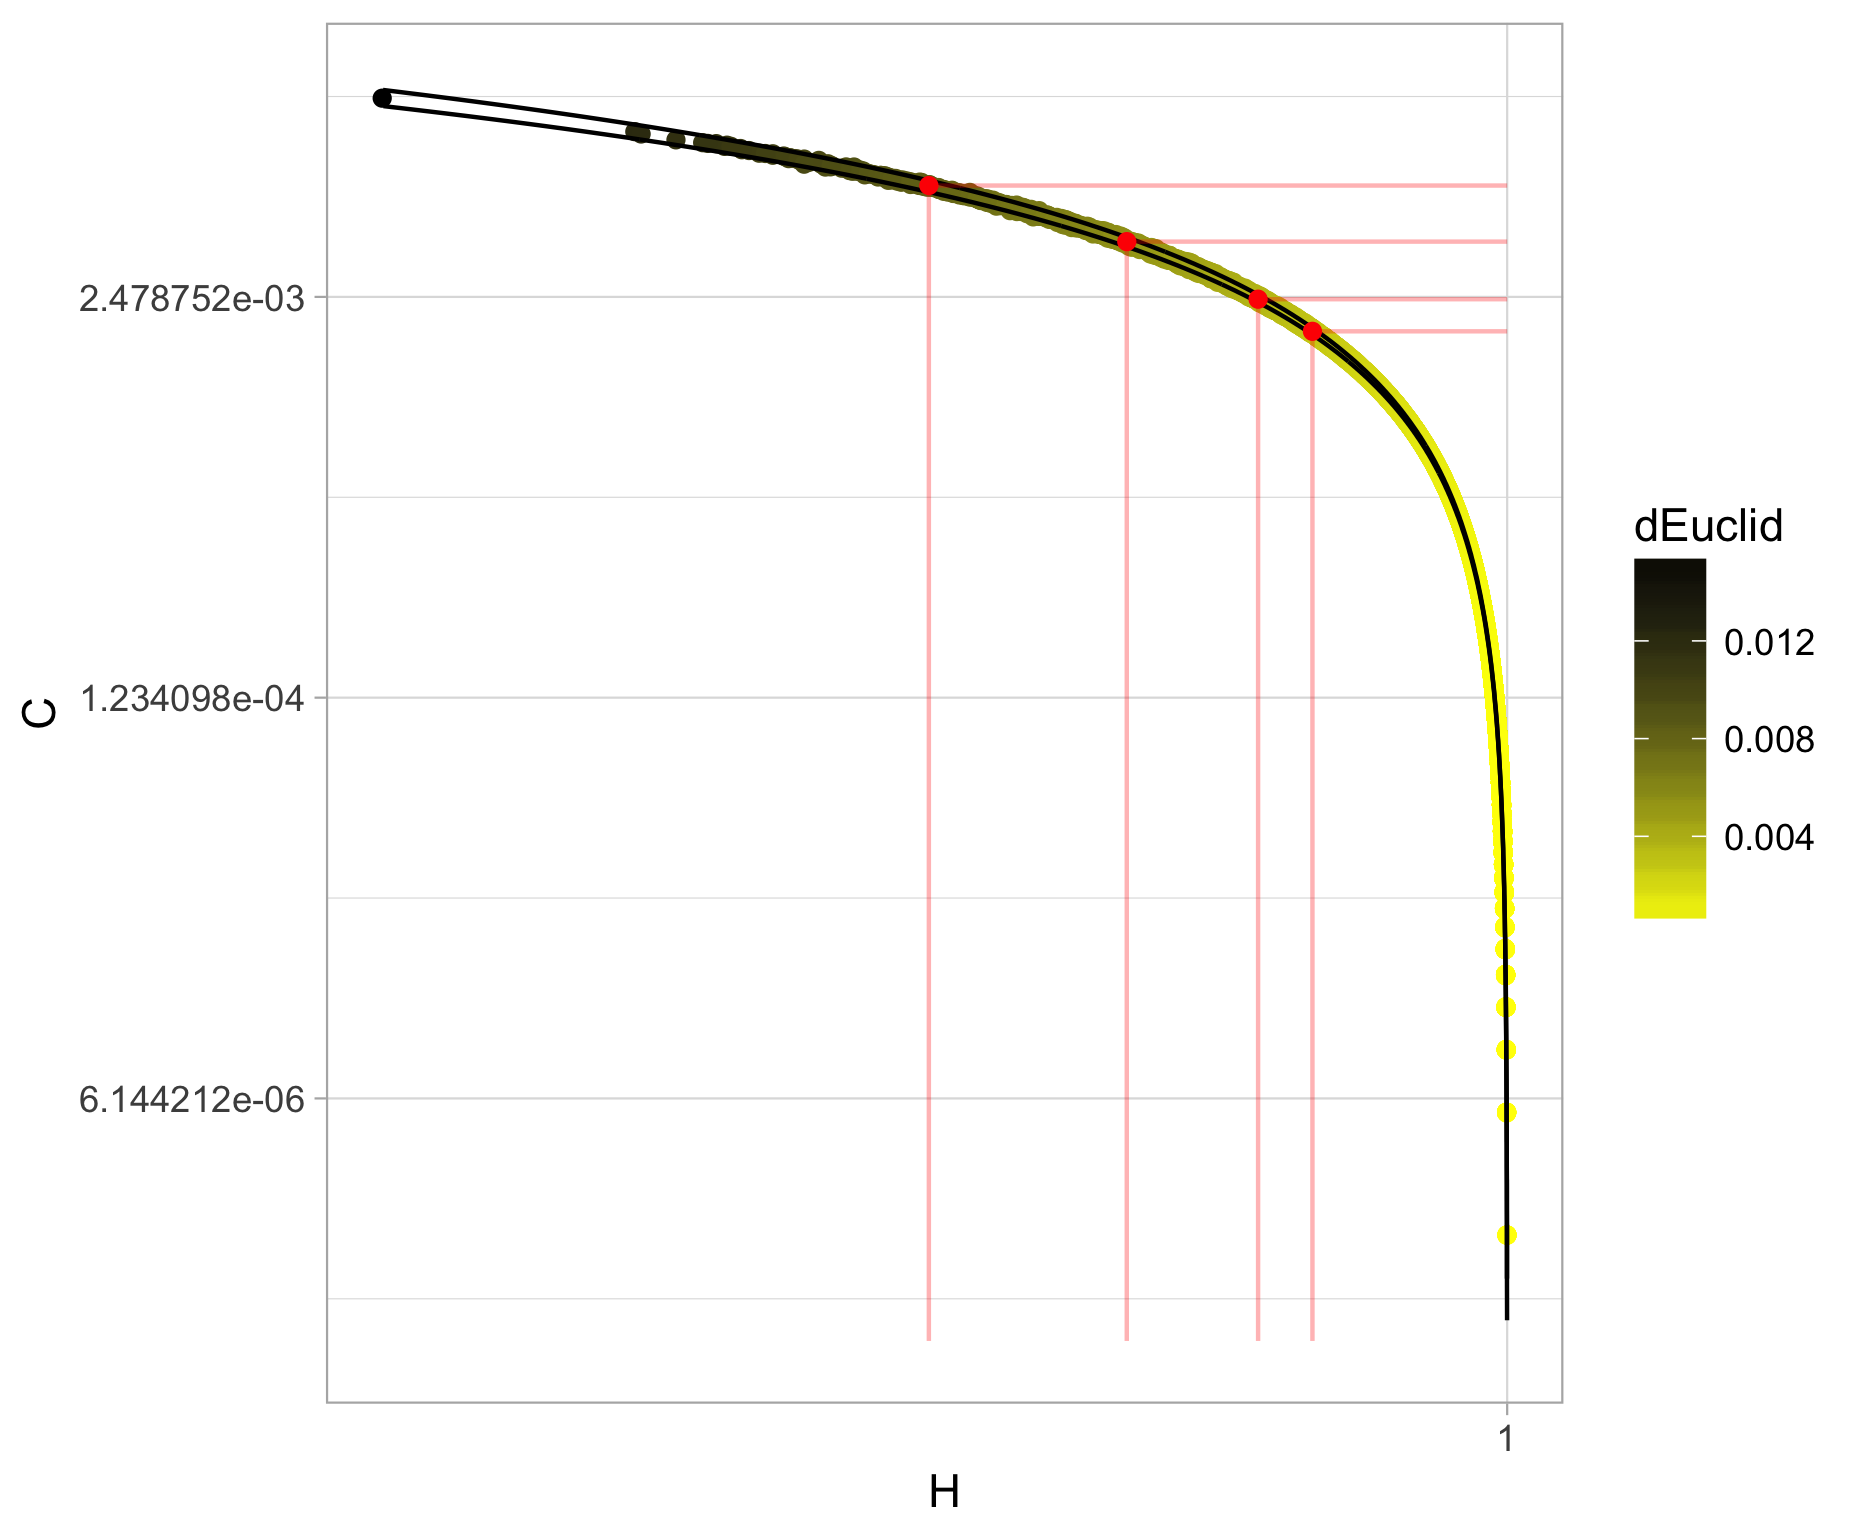
\includegraphics[width=.48\linewidth]{scatter1000D3t1_log}}
\caption{Diagramas de dispersão das sequências aleatórias para o caso $N=1.000$, $D=3$ e $\tau=1$.}\label{Fig:AleattD3tau1}
\end{figure}

\begin{figure}
\centering
\subfigure[Escala linear\label{Fig:scatter50kD6t50}]{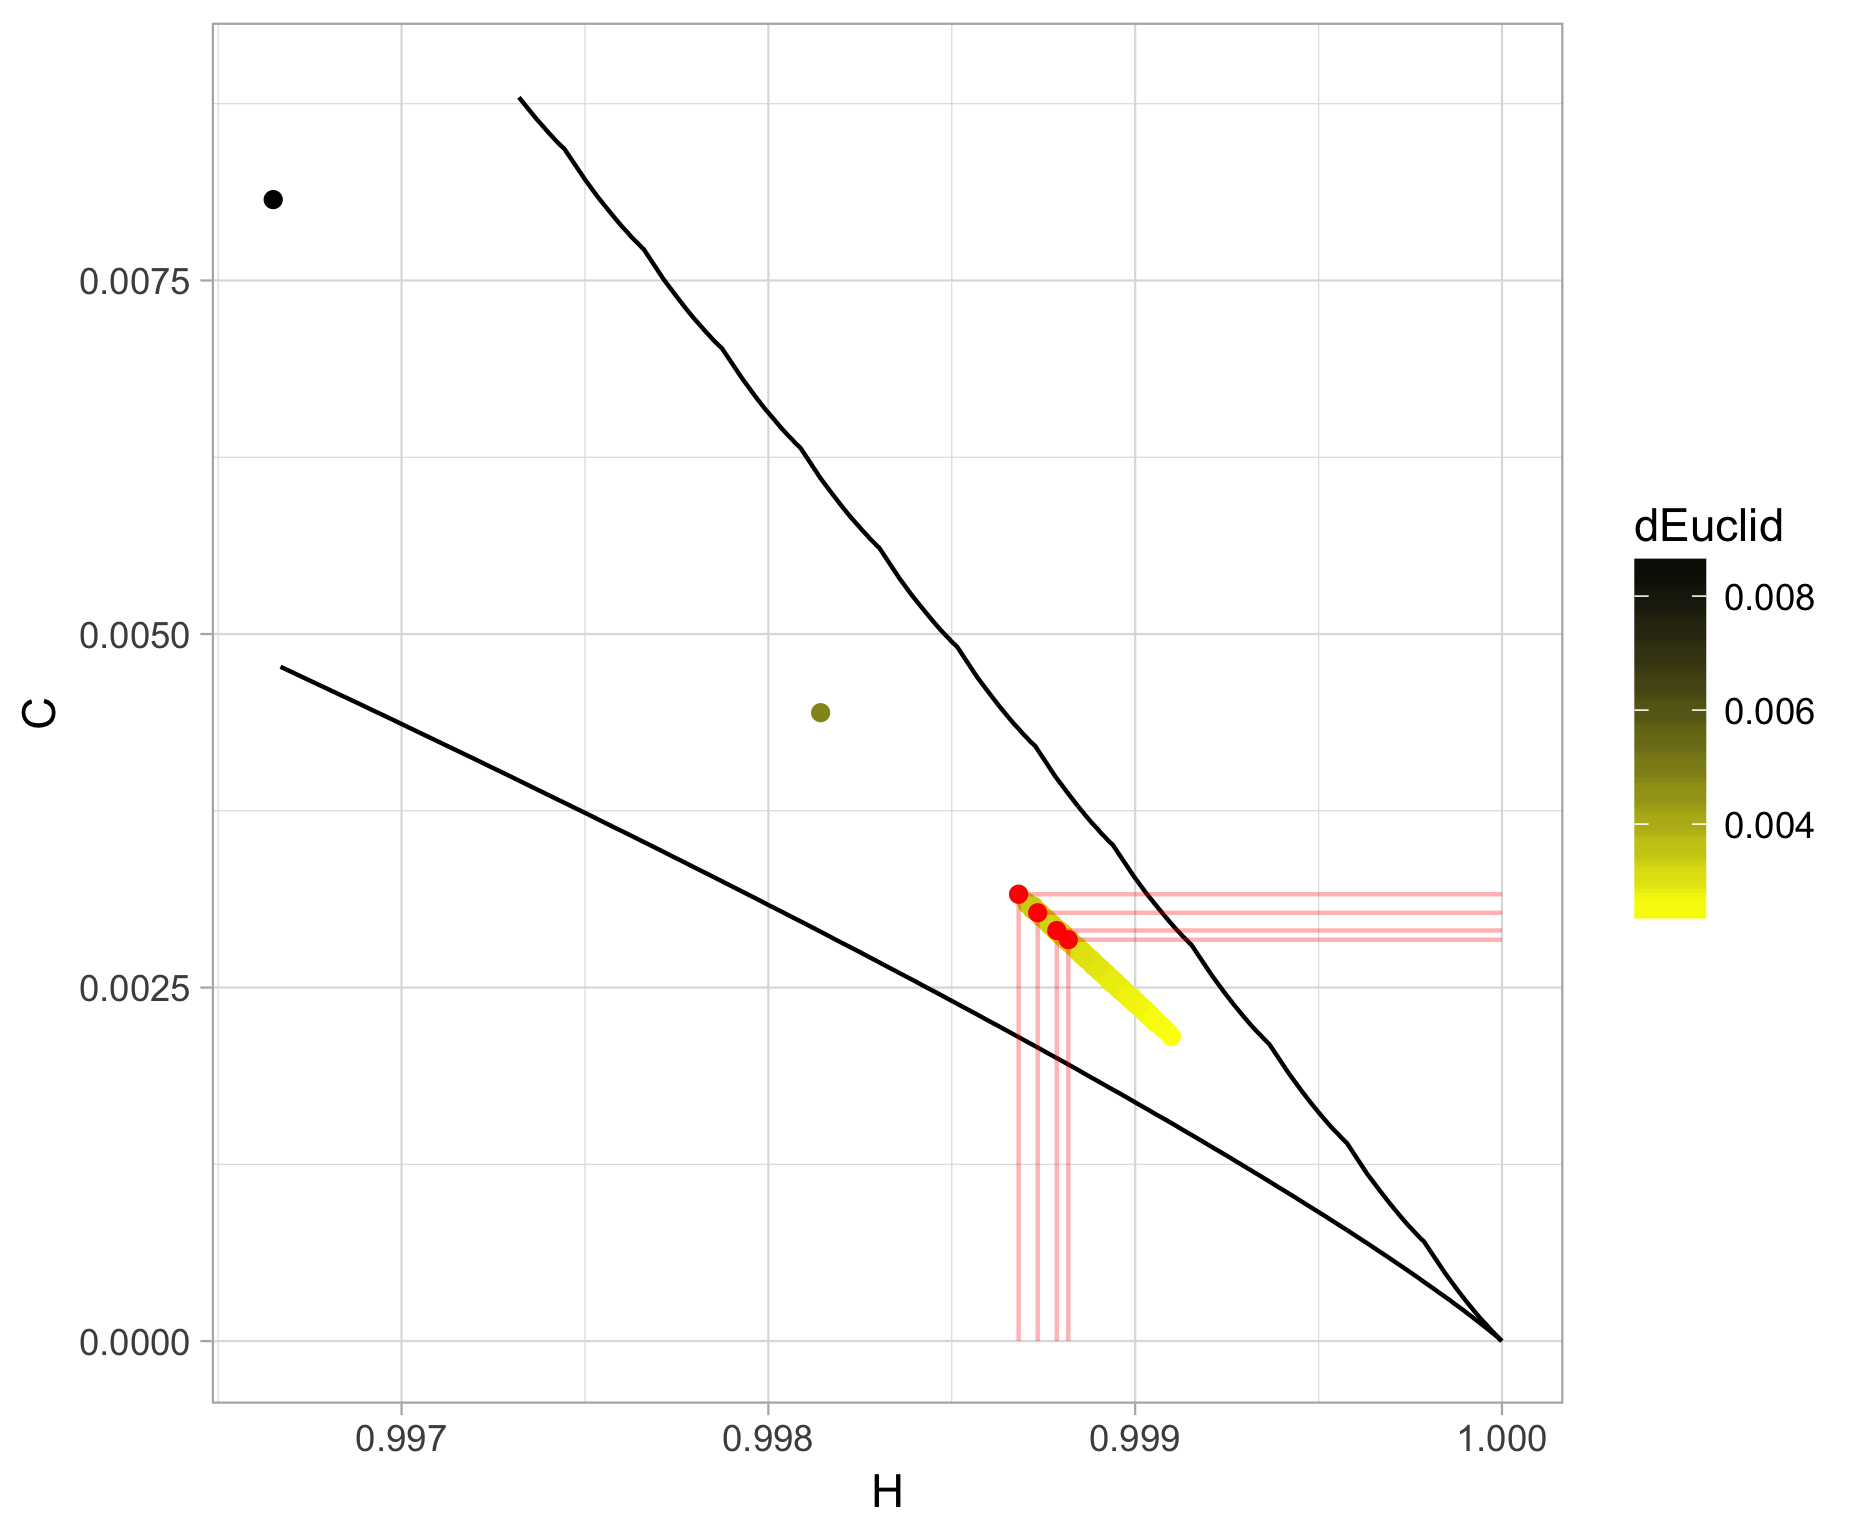
\includegraphics[width=.48\linewidth]{scatter50kD6t50}}
\subfigure[Escala logarítmica\label{Fig:scatter50kD6t50_log}]{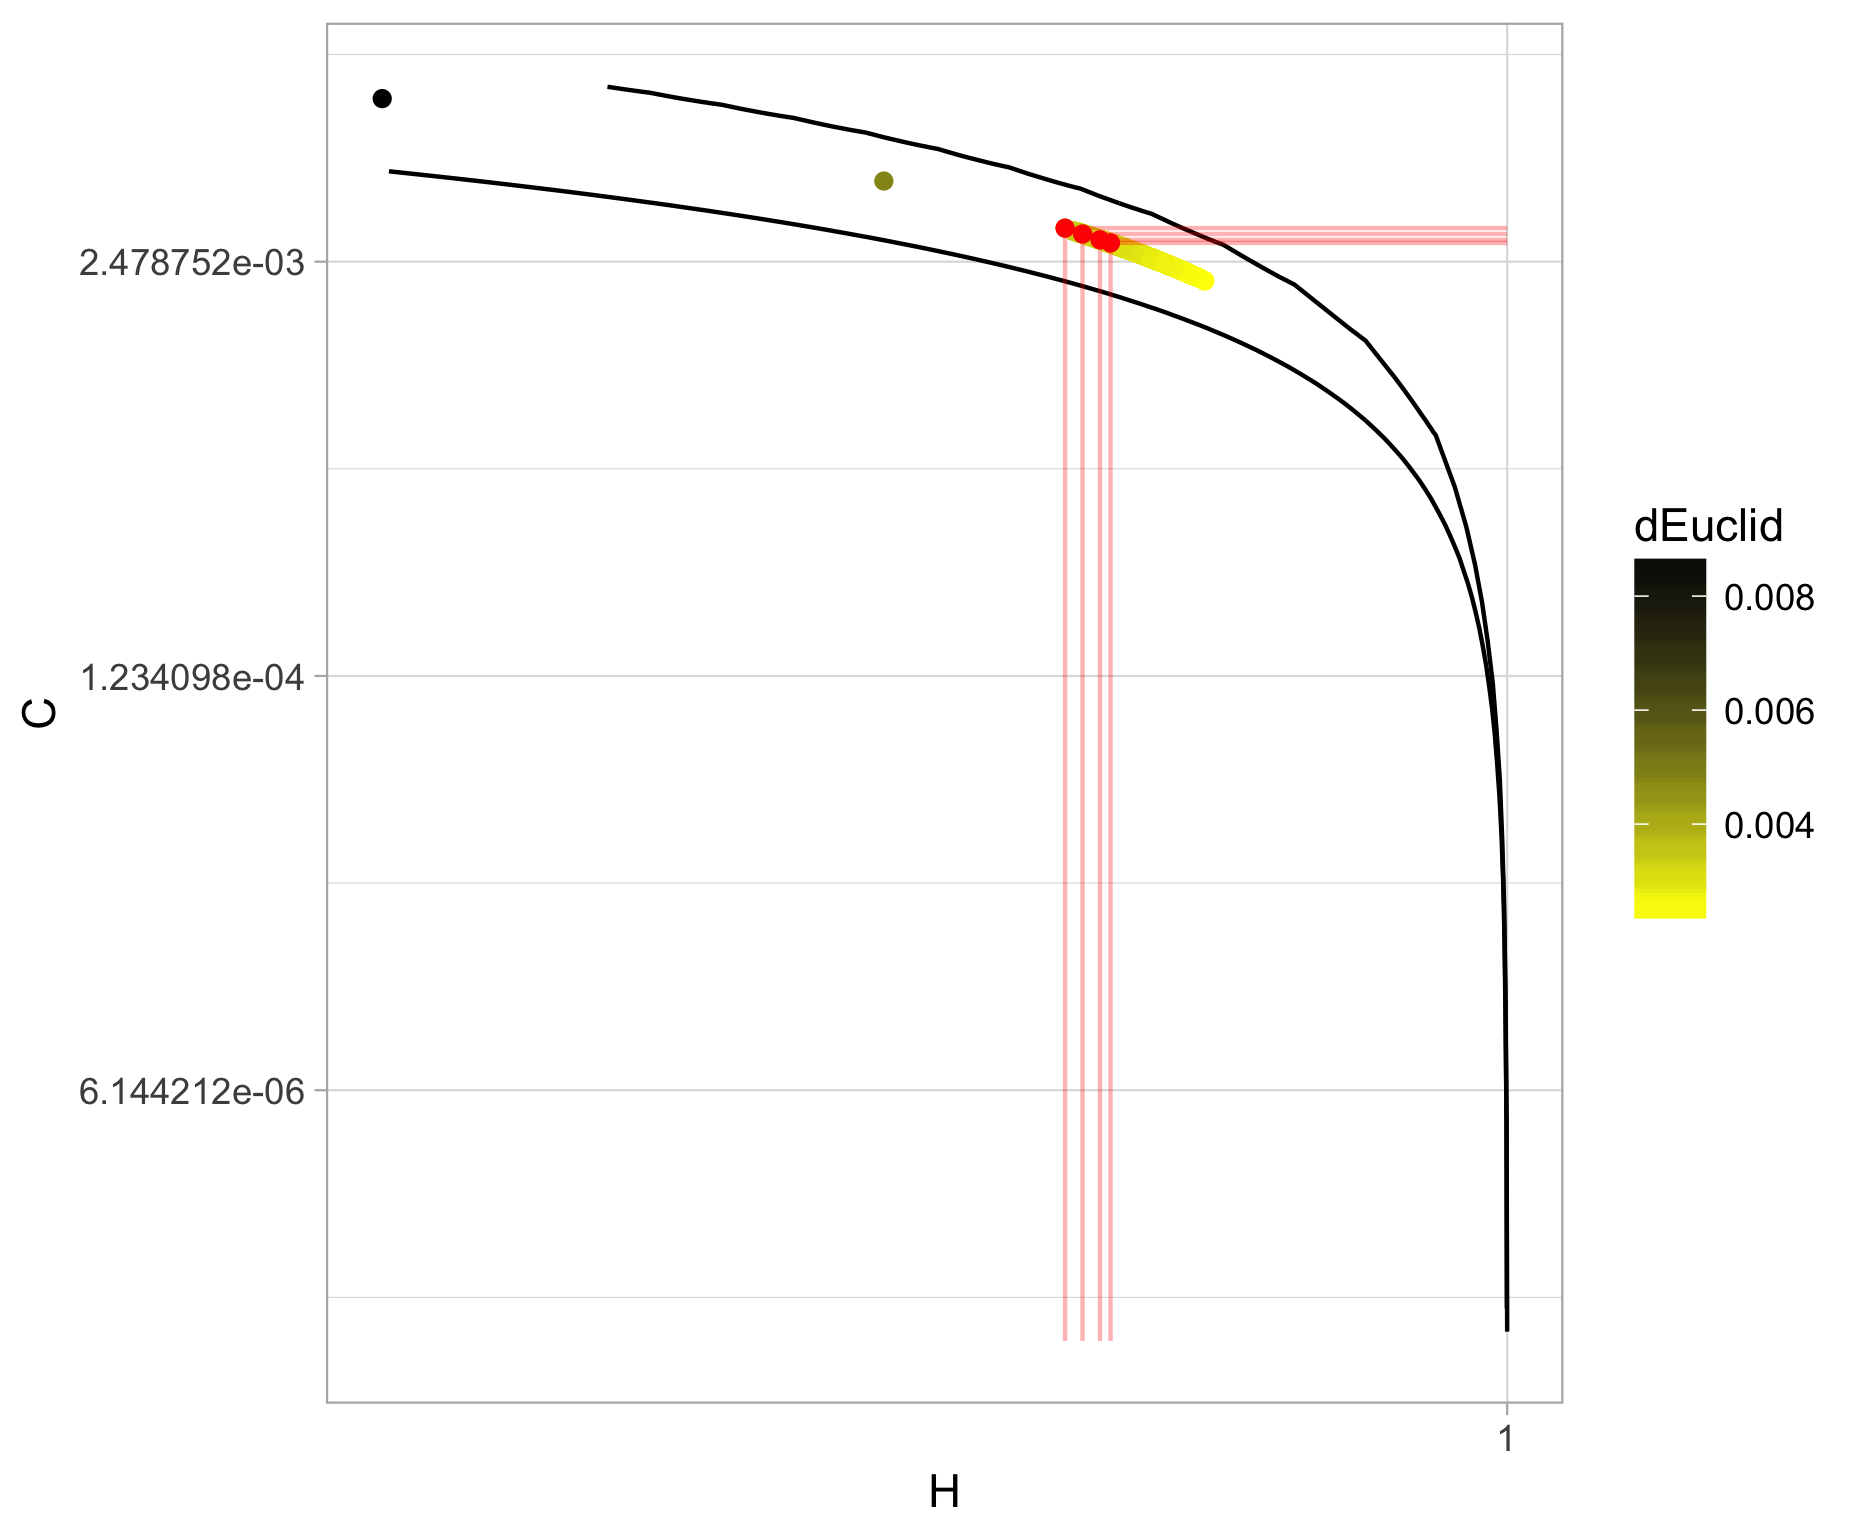
\includegraphics[width=.48\linewidth]{scatter50kD6t50_log}}
\caption{Diagramas de dispersão das sequências aleatórias para o caso $N=50.000$, $D=6$ e $\tau=50$.}\label{Fig:QuantD3tau10log}
\end{figure}

\begin{figure}[hbt]
	\centering
	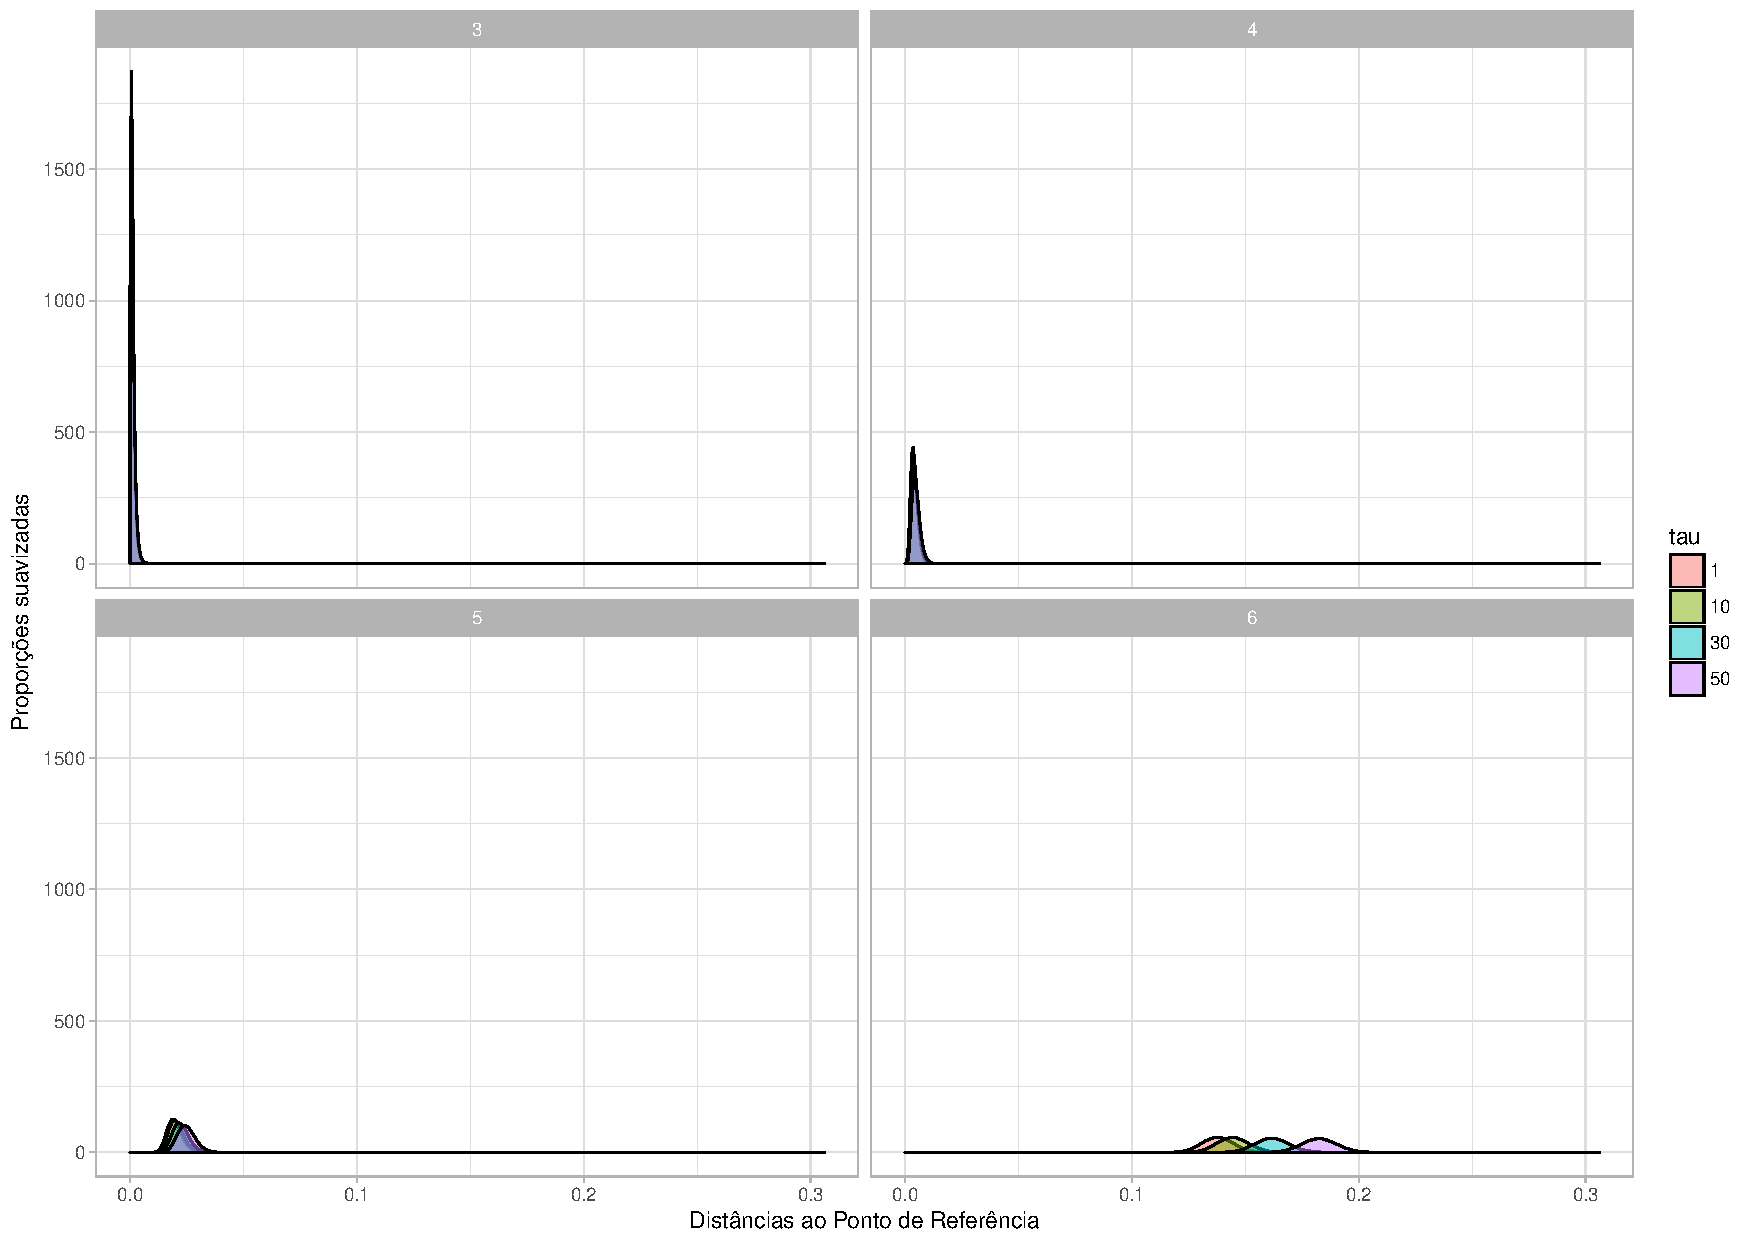
\includegraphics[width=\linewidth]{HistoDistanciasRandTodas}
	\caption{Histogramas suavizados das distâncias euclidianas dos padrões ao ponto de referência, para $D\in\{3,4,5,6\}$ (colunas) e $\tau\in\{1,10,30,50\}$ (linhas).}\label{Fig:HistoDistanciasRandTodas}
\end{figure}



\section{Análise das sequências de rádio}


Antes de analisar os diagramas de dispersão, analisaremos a distribuição empírica das distâncias ao ponto de referência.

A figura~\ref{Fig:HistoDistanciasRandTodas} sugere que o comportamento das distâncias euclidianas ao ponto de referência muda conforme o tamanho do padrão $D$ varia.
Além disso, também são perceptíveis mudanças de comportamento em funçao do \textit{lag} $\tau$ quando $D=5,6$.

No que segue analisaremos o comportamento dessas distâncias em detalhes.


\begin{figure}
	\centering
	%\subfigure[Escala linear\label{Fig:ScatterRandD3tau1}]{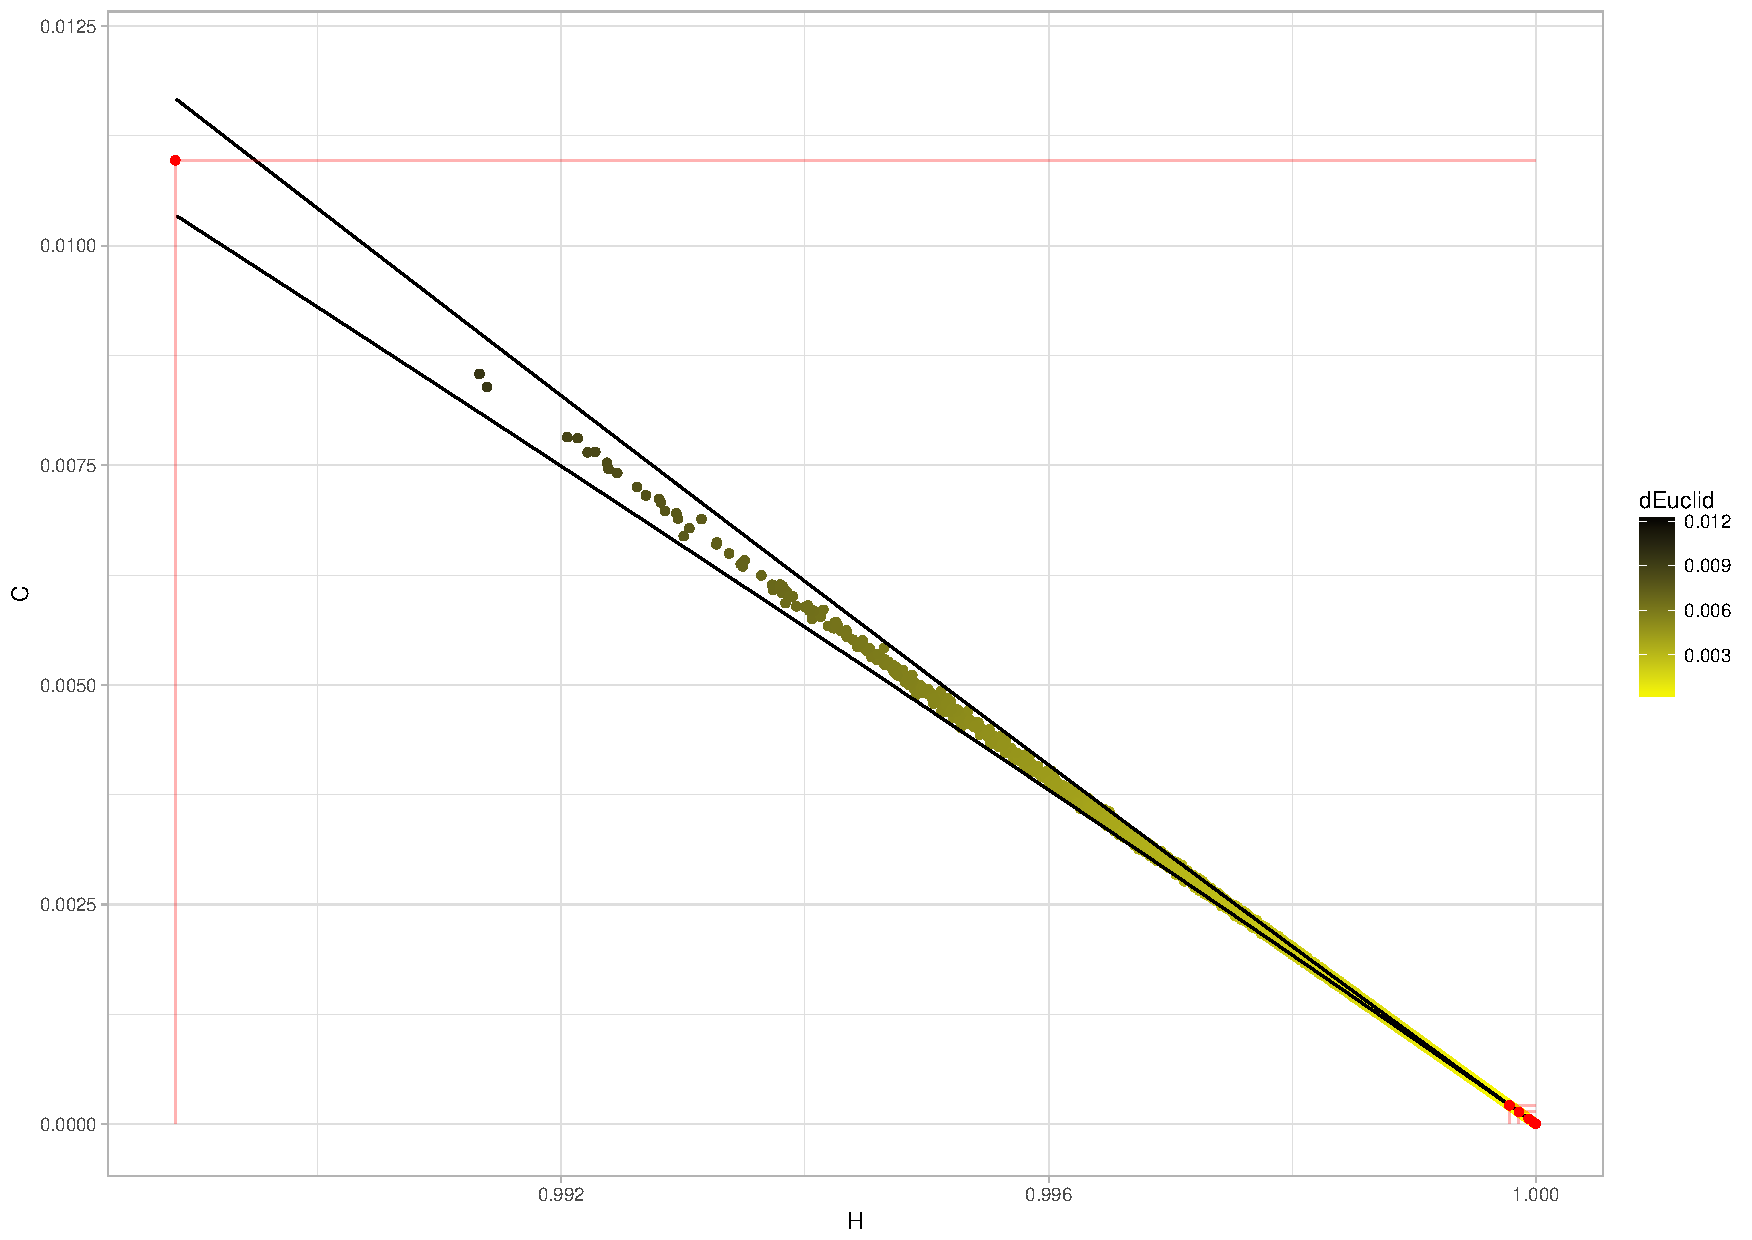
\includegraphics[width=.48\linewidth]{ScatterRandD3tau1}}
	\subfigure[Escala logarítmica\label{Fig:ScatterRandD3tau1log}]{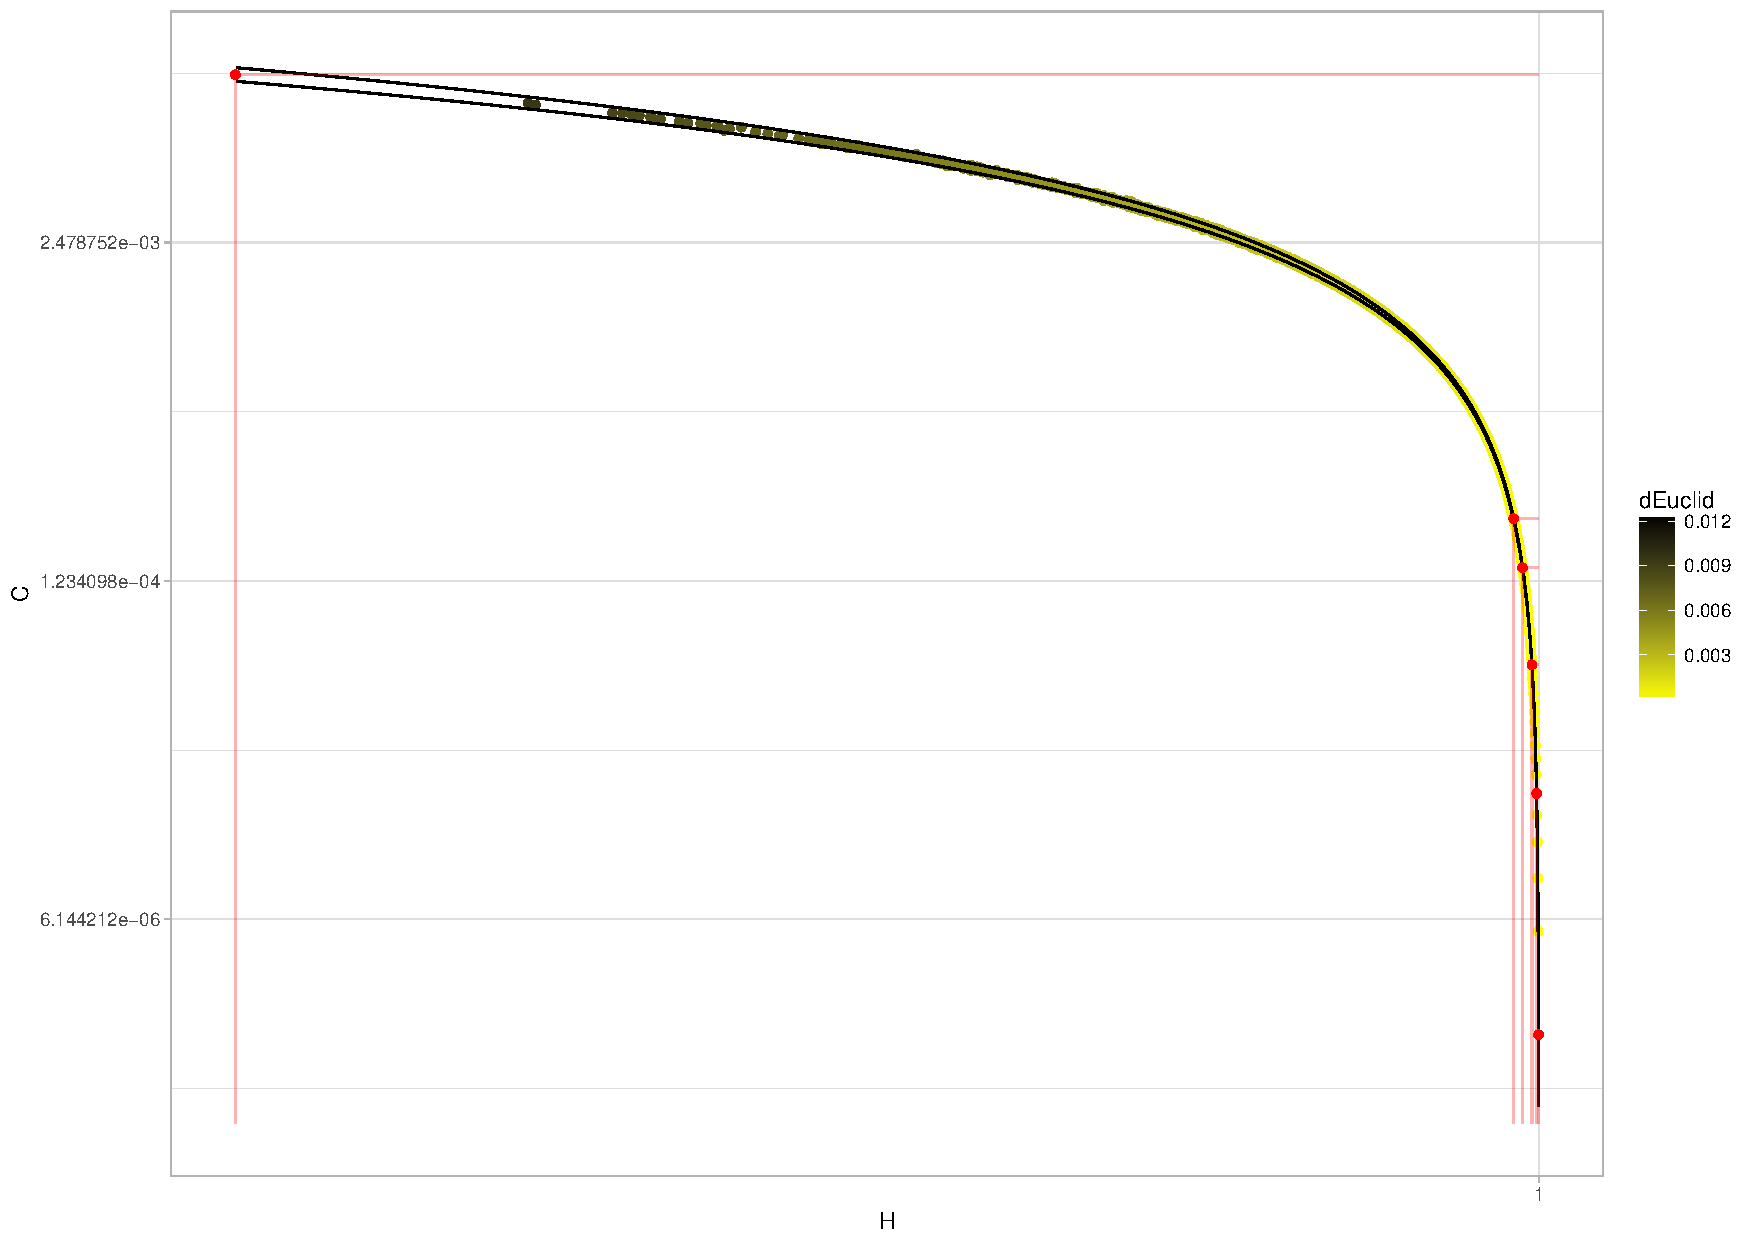
\includegraphics[width=.48\linewidth]{ScatterRandD3tau1log}}
	\caption{Diagramas de dispersão das sequências de rádio para o caso $D=3$ e $\tau=1$.}\label{Fig:RadioD3tau1}
\end{figure}

\begin{figure}
	\centering
%	\subfigure[Escala linear\label{Fig:ScatterRandD3tau10}]{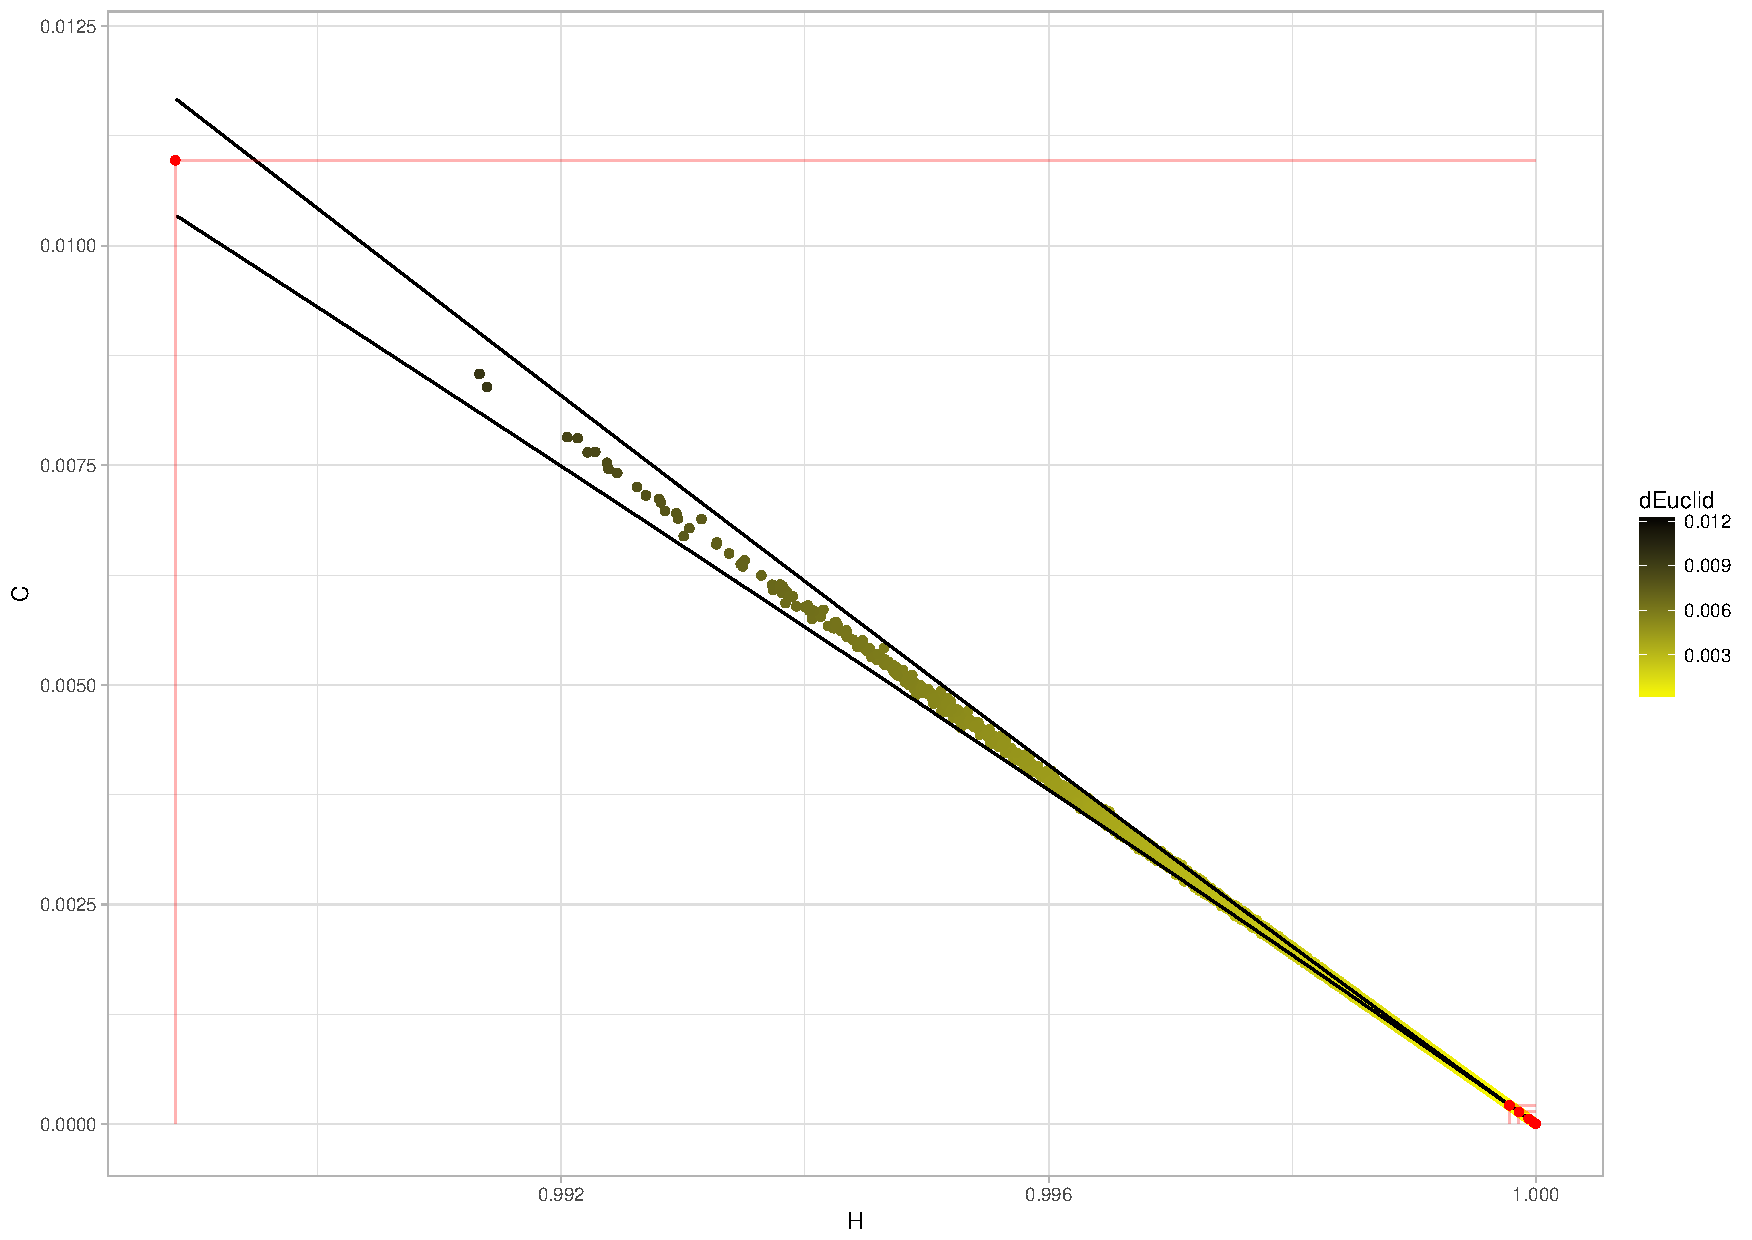
\includegraphics[width=.48\linewidth]{ScatterRandD3tau1}}
	\subfigure[Escala logarítmica\label{Fig:ScatterRandD3tau10log}]{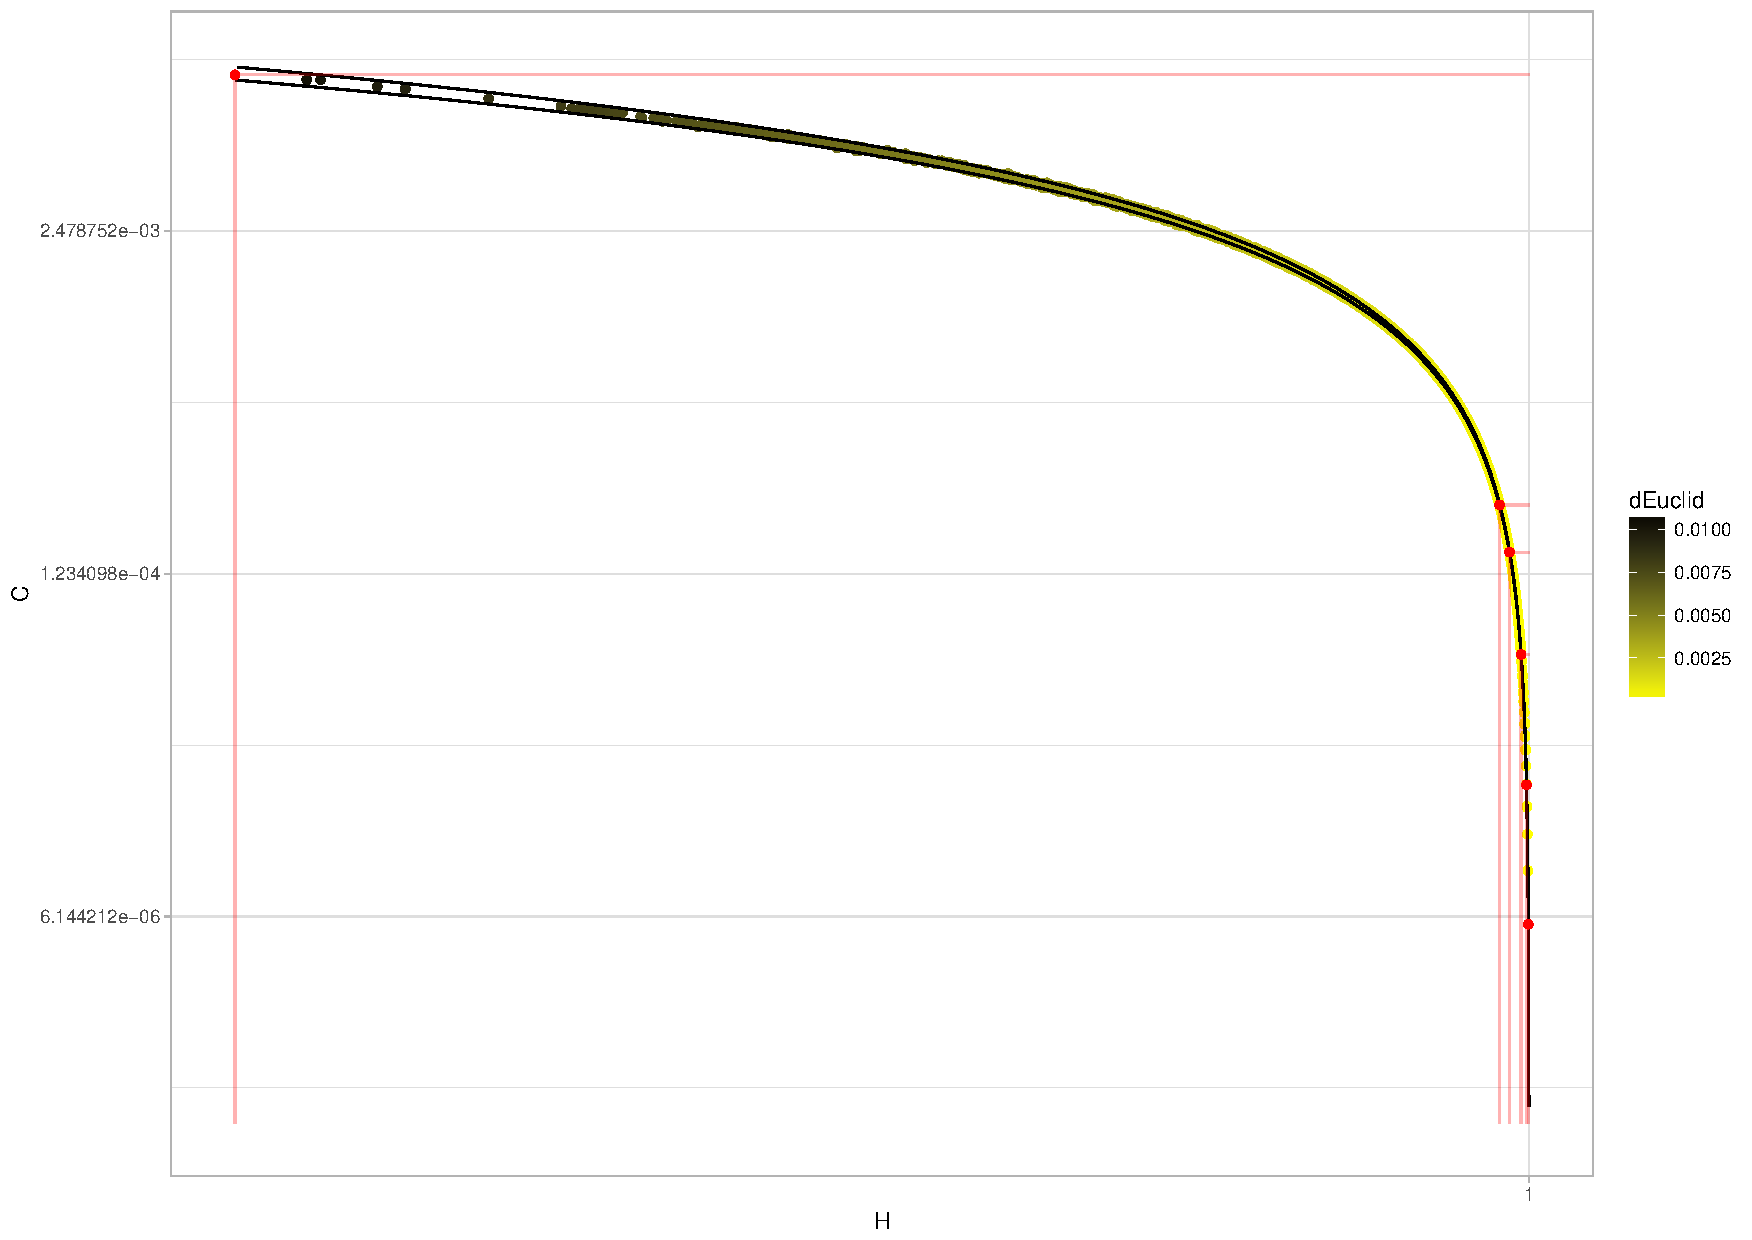
\includegraphics[width=.48\linewidth]{ScatterRandD3tau10log}}
	\caption{Diagramas de dispersão das sequências quânticas para o caso $D=3$ e $\tau=10$.}\label{Fig:QuantD3tau10}
\end{figure}


\section{Análise das sequências Mersenne-Twister}

%\begin{figure}
%	\centering
%	%	\subfigure[Escala linear\label{Fig:ScatterRandD3tau10}]{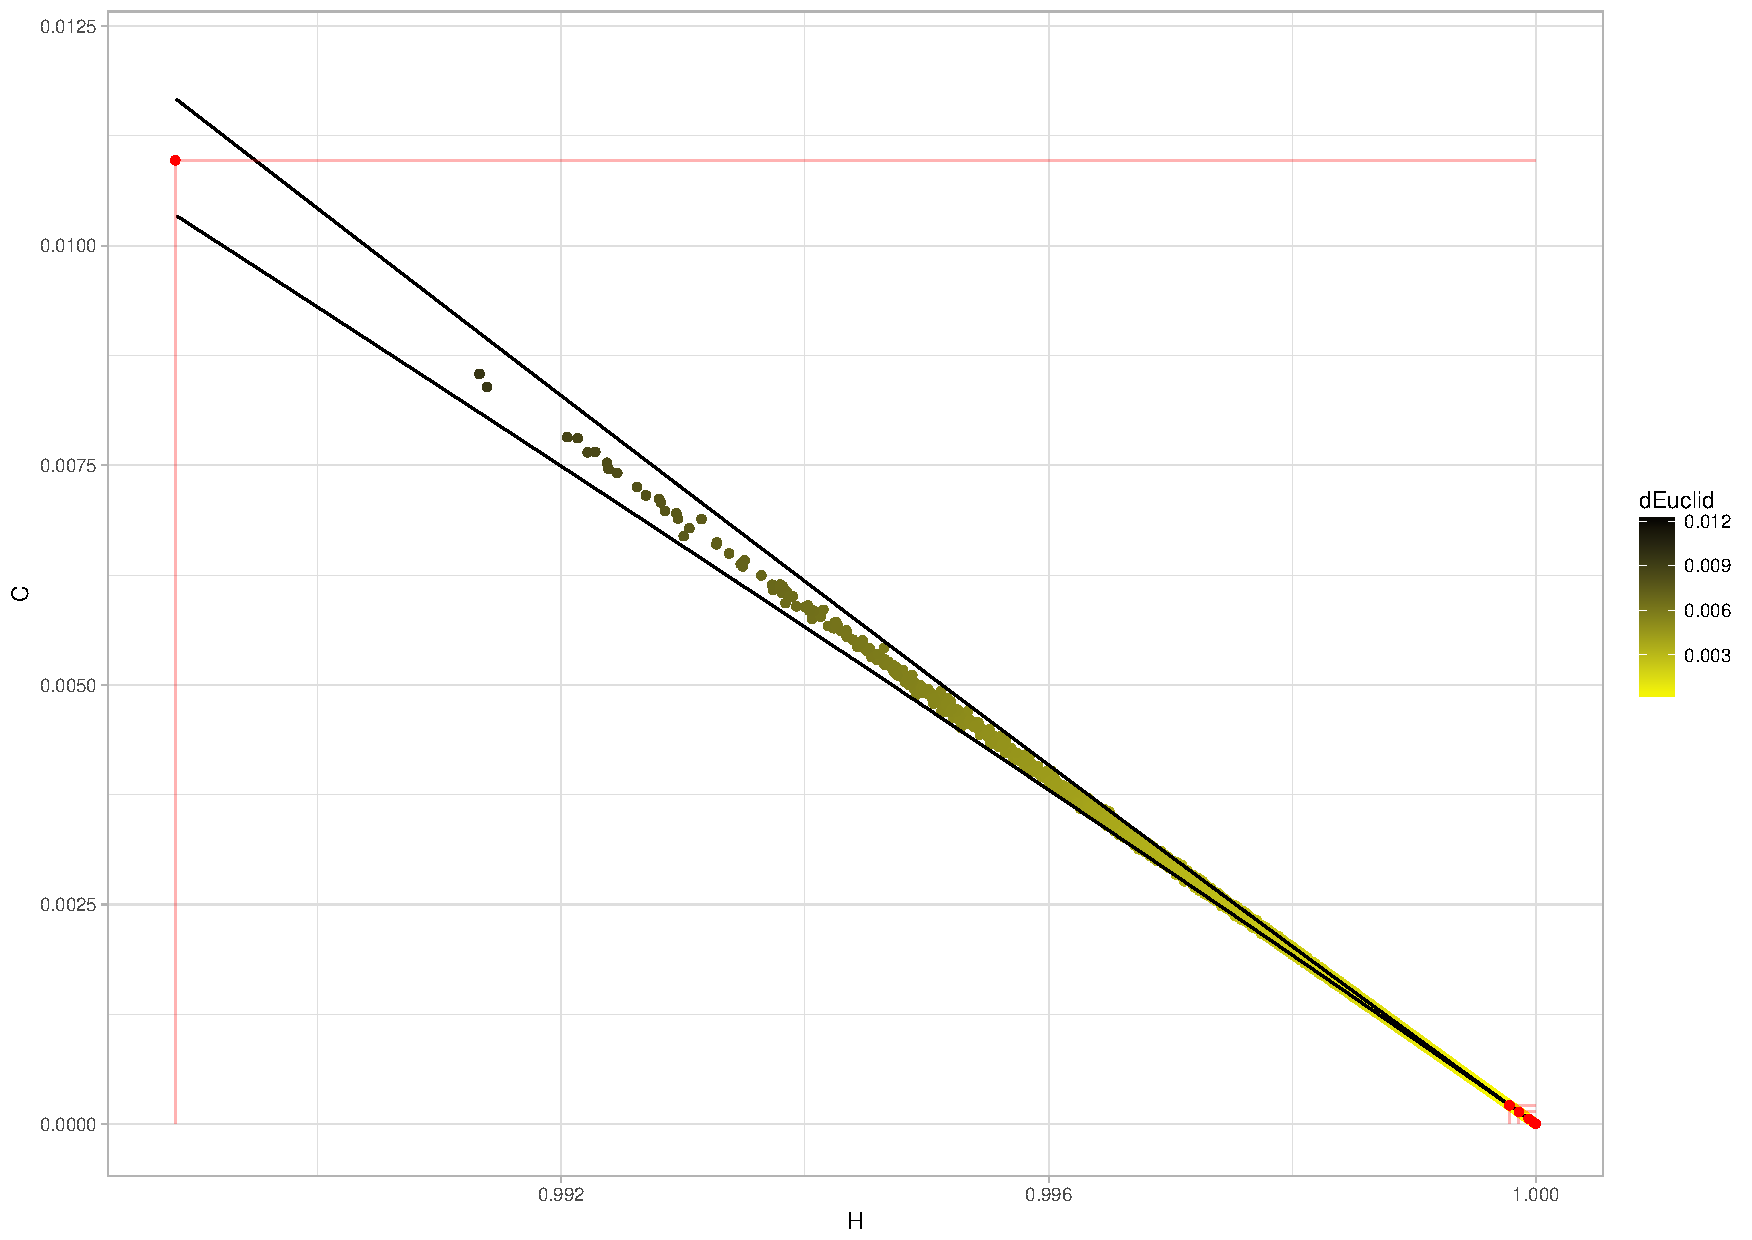
\includegraphics[width=.48\linewidth]{ScatterRandD3tau1}}
%	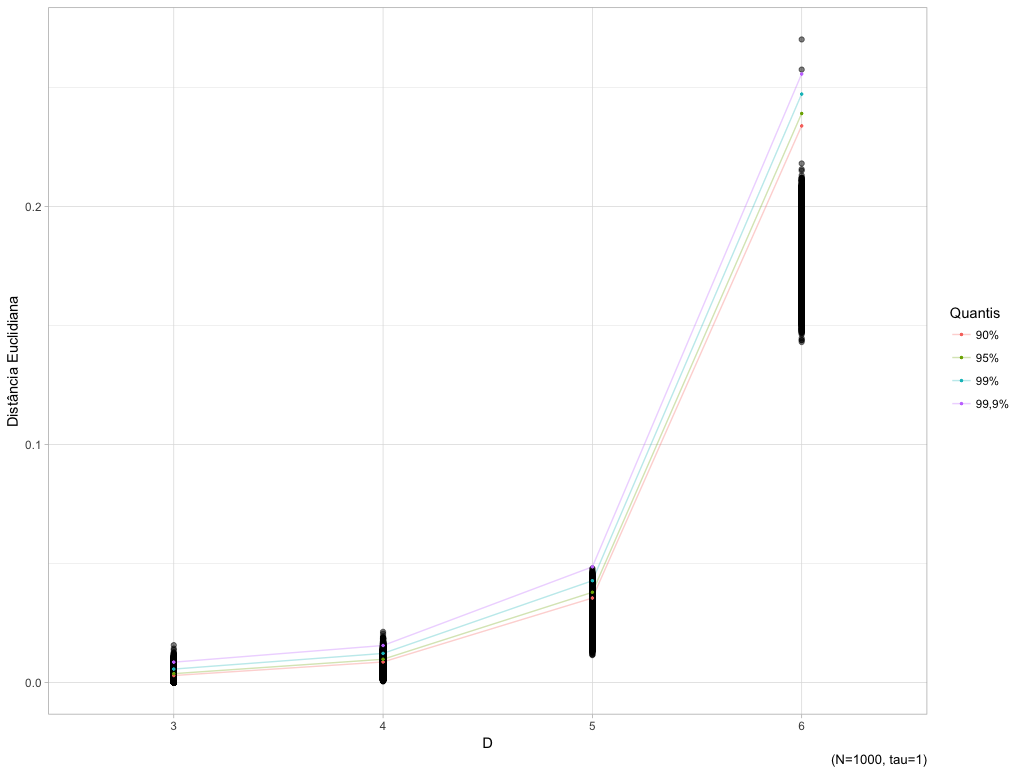
\includegraphics[width=.8\linewidth]{Conf_Int_1k_T1}
%	\caption{Intervalos de confiança para o caso $N=1000$ e $\tau=1$.}\label{Fig:Conf_Int_1k_T1}
%\end{figure}

\section{Análise das regiões de confiança}

%% N=1.000
\begin{figure}
	\centering
	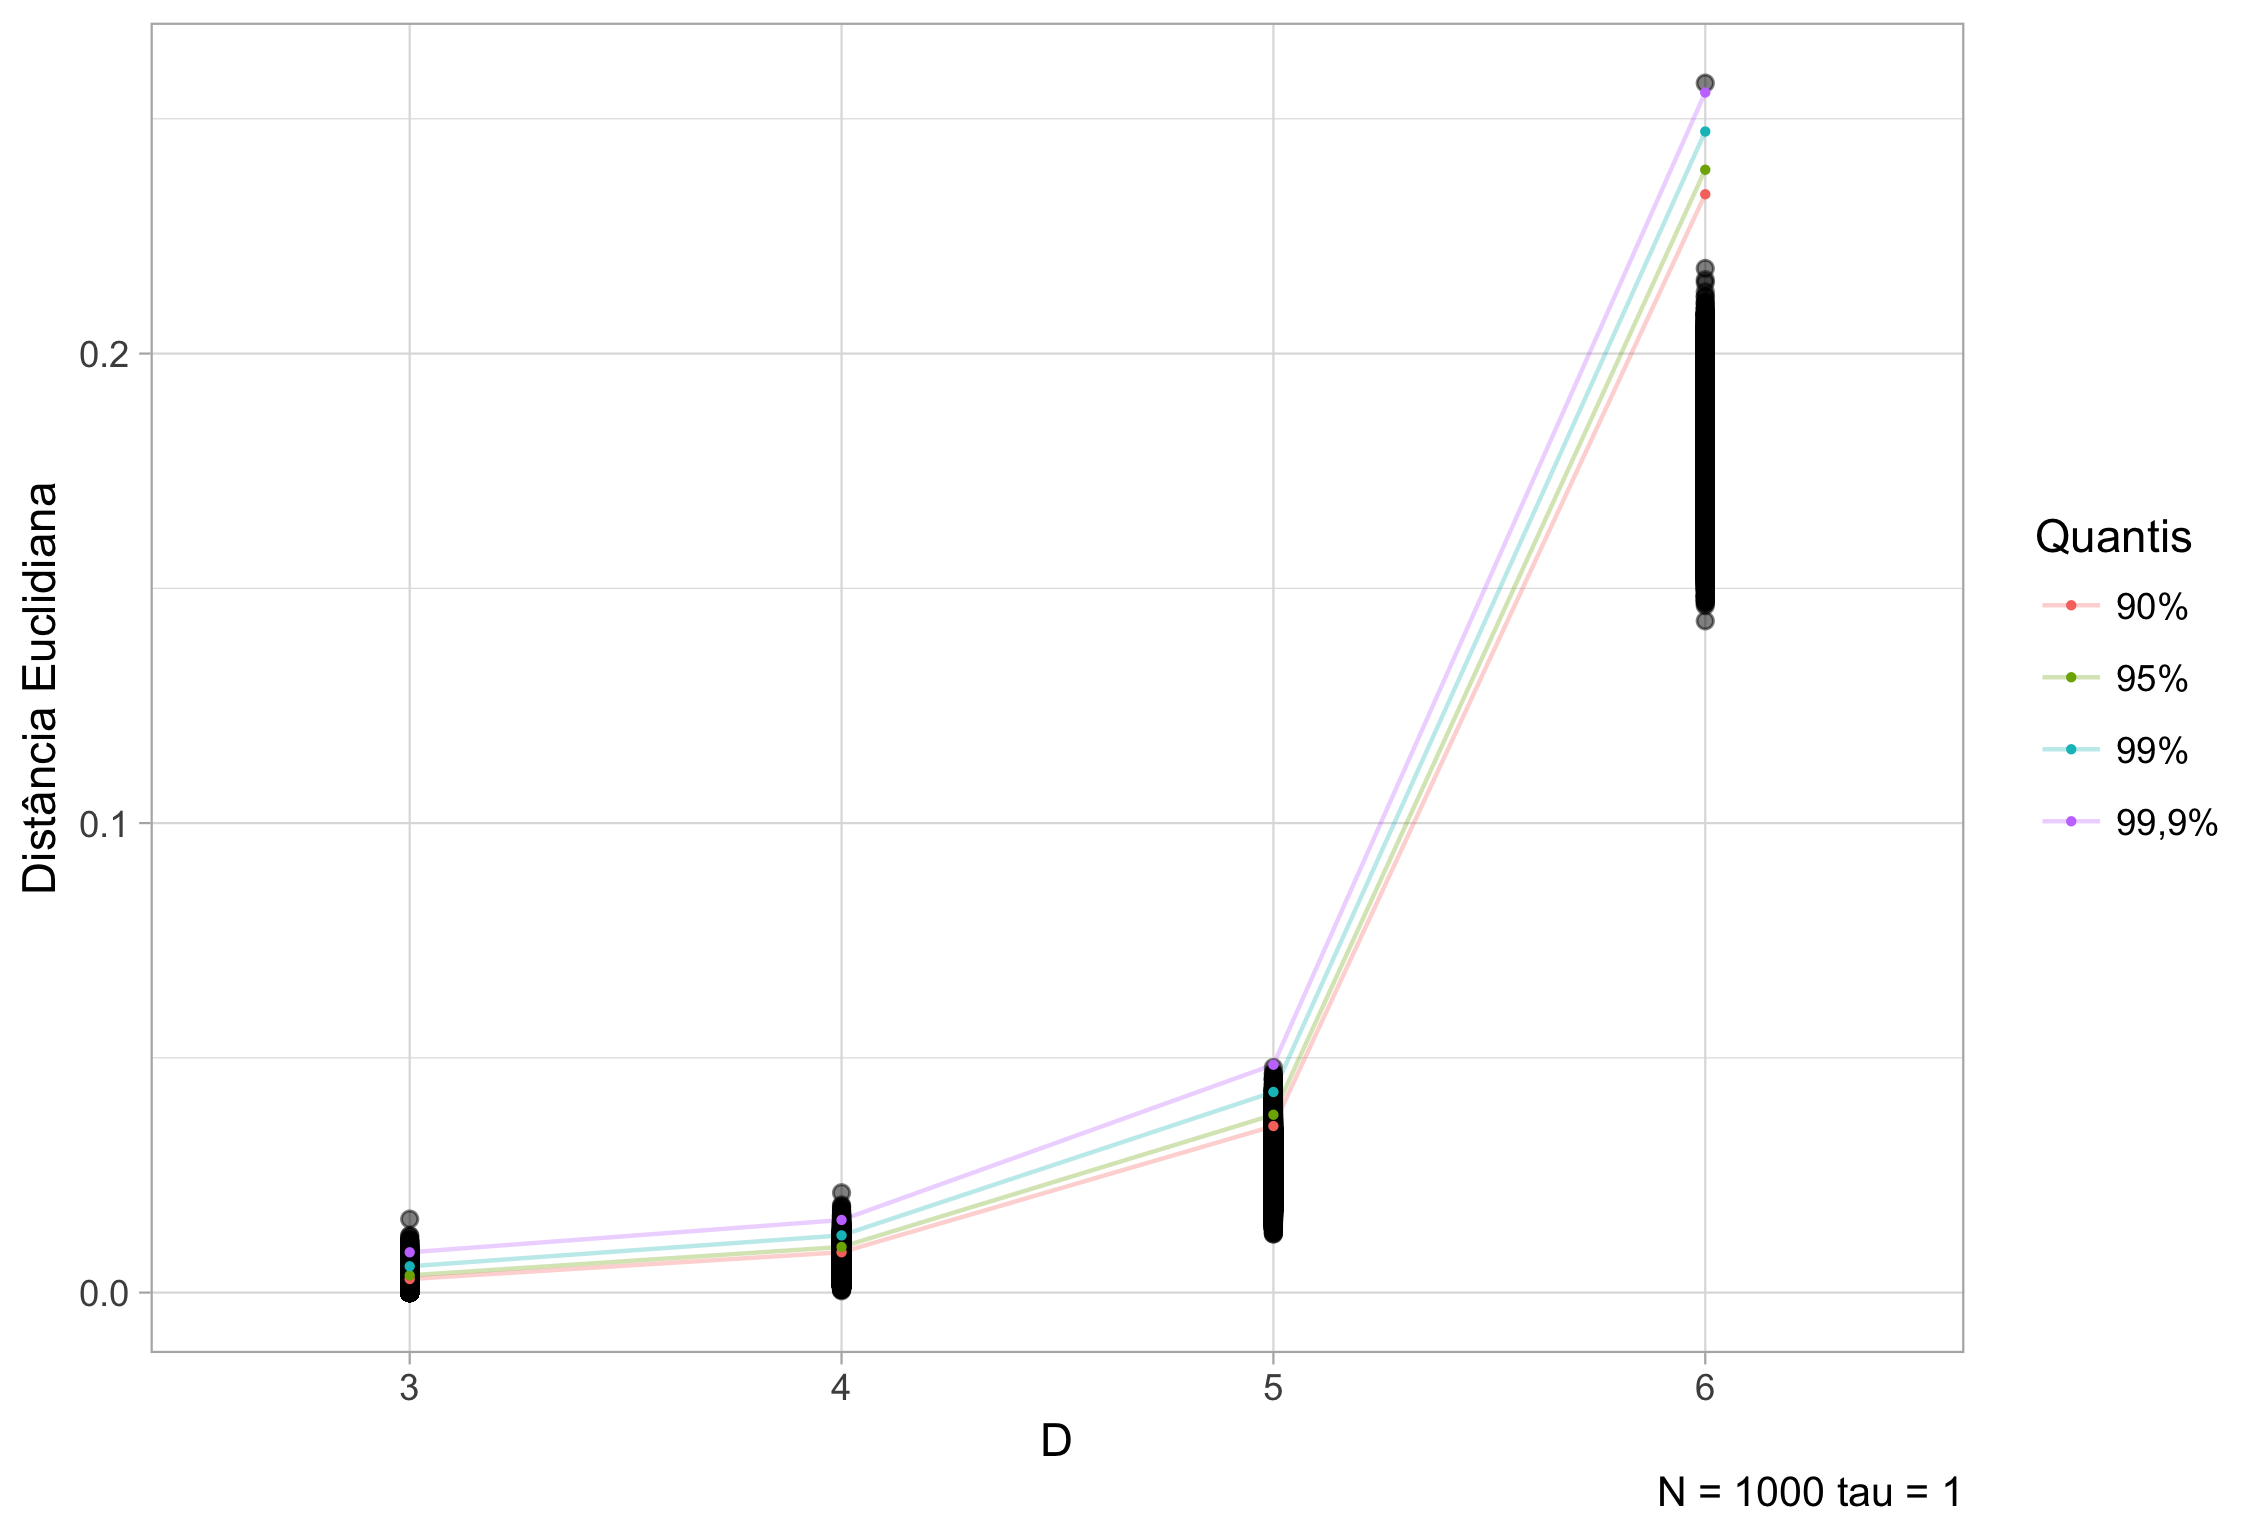
\includegraphics[width=1\linewidth]{Conf_Int_1k_T1_noMT}
	\caption{Intervalos de confiança para o caso $N=1.000$ e $\tau=1$.}\label{Fig:Conf_Int_1k_T1}
\end{figure}

\begin{figure}
	\centering
	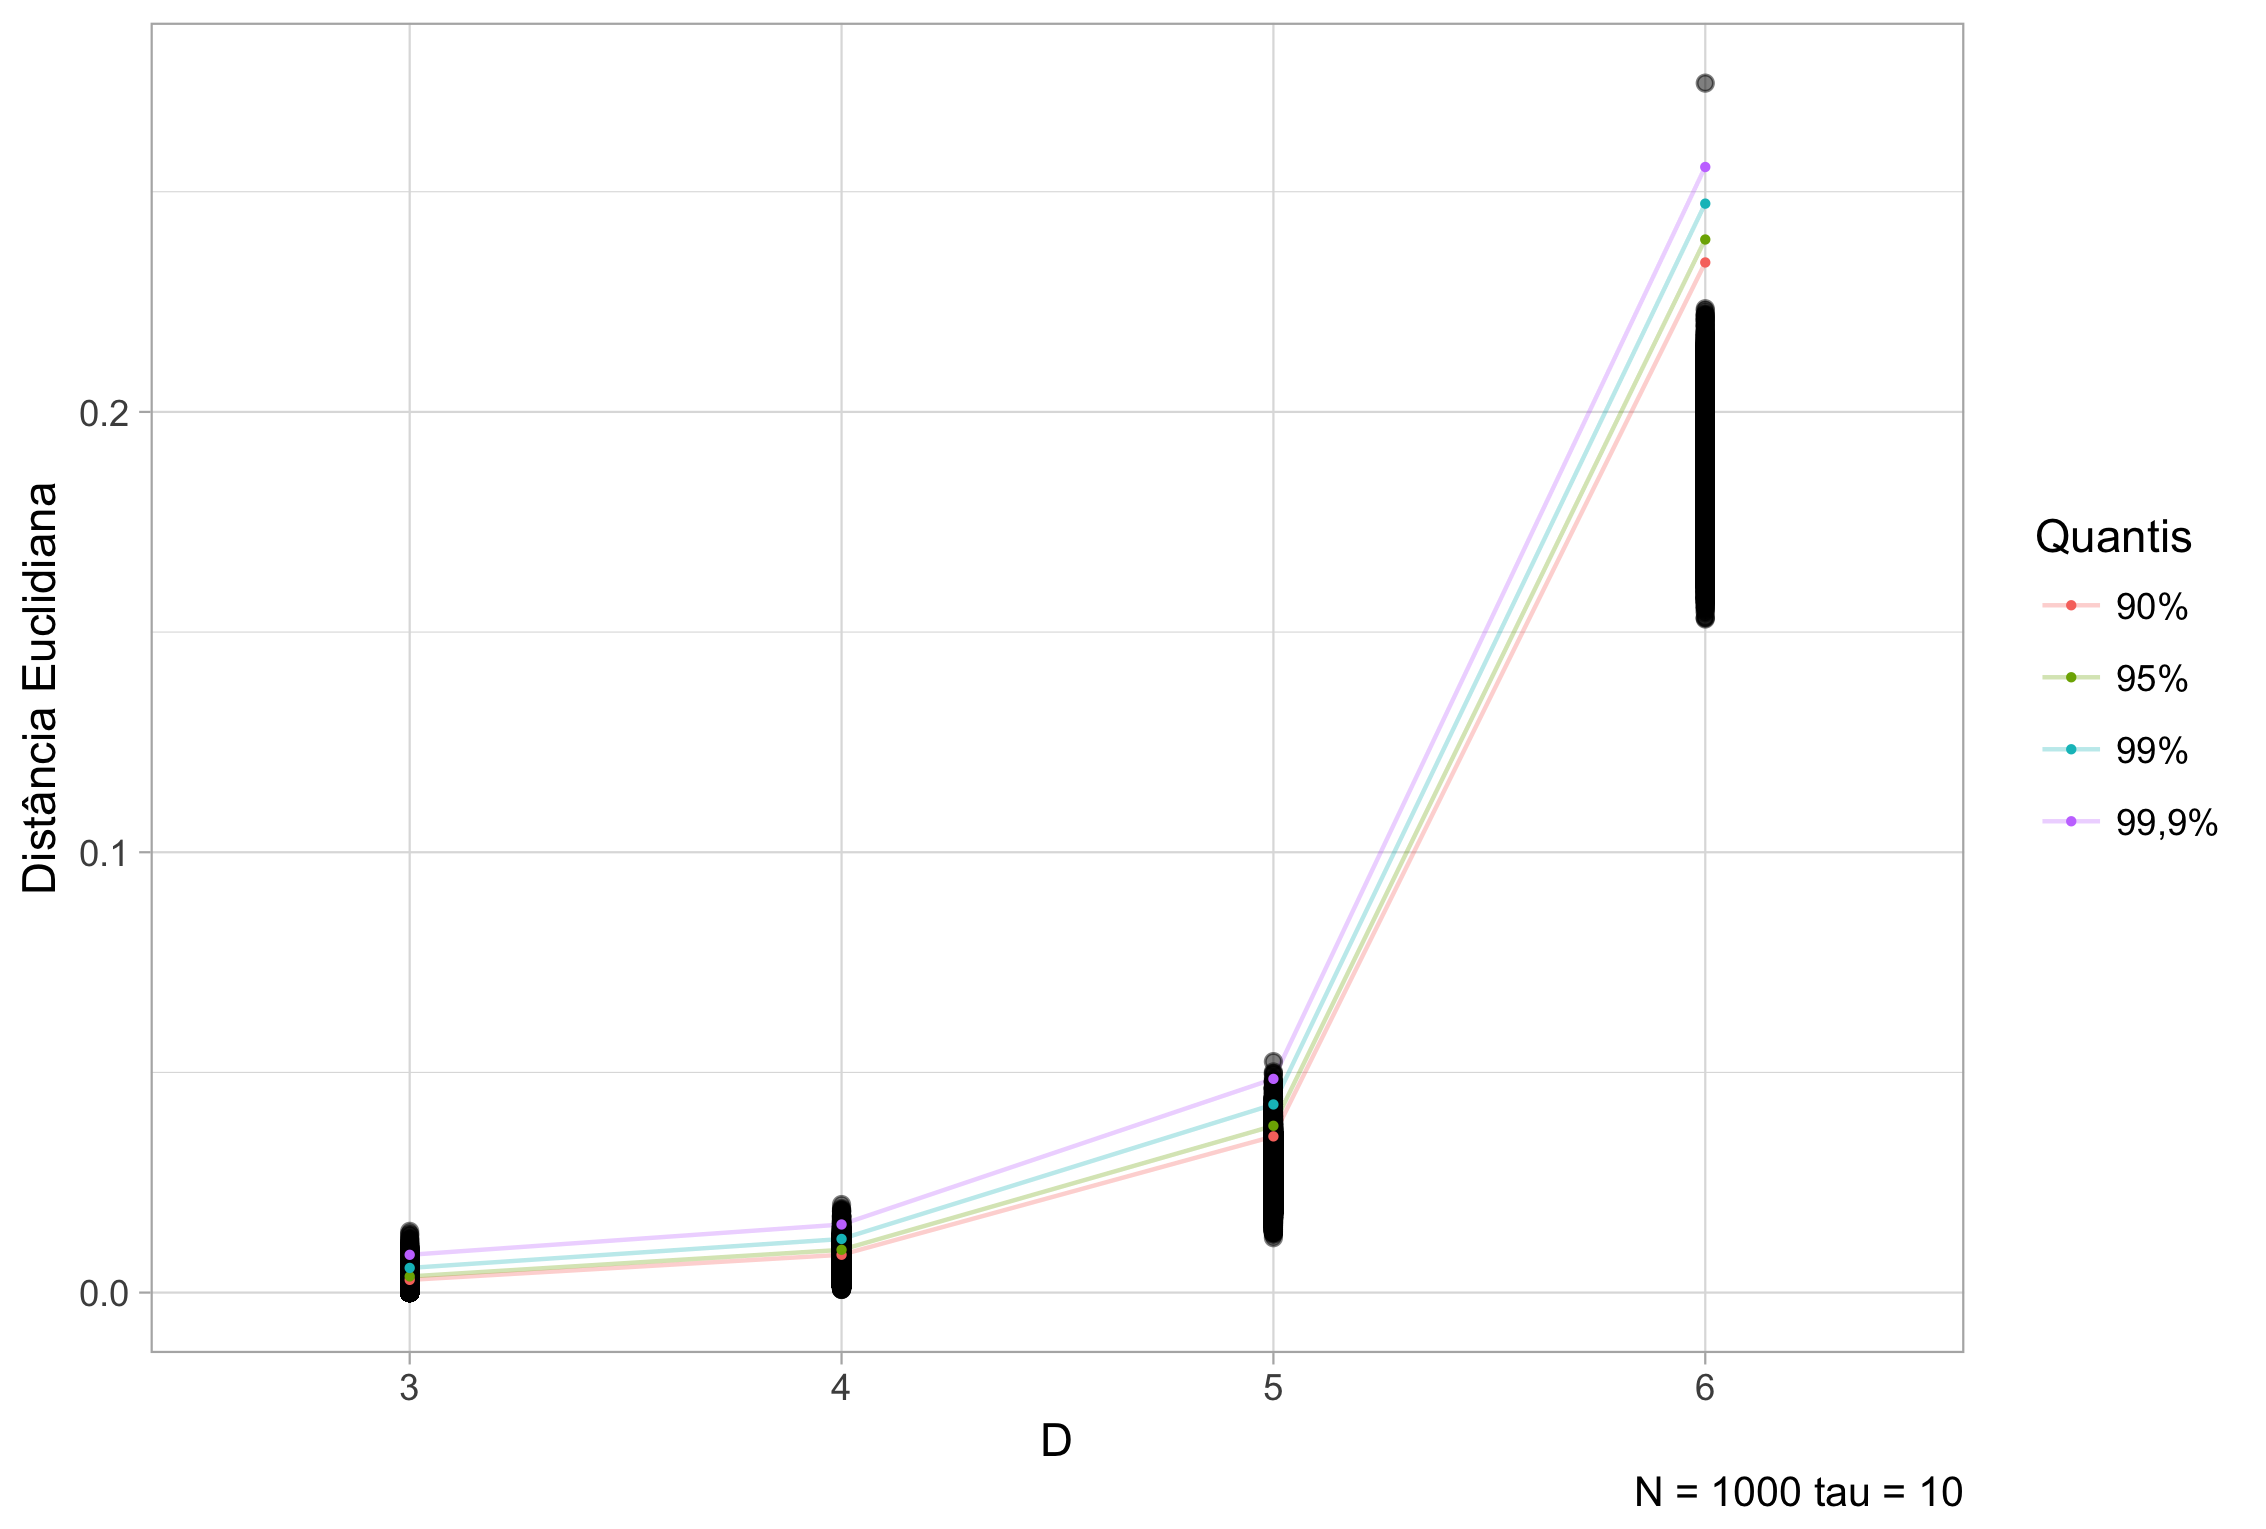
\includegraphics[width=1\linewidth]{Conf_Int_1k_T10_noMT}
	\caption{Intervalos de confiança para o caso $N=1.000$ e $\tau=10$.}\label{Fig:Conf_Int_1k_T10}
\end{figure}

\begin{figure}
	\centering
	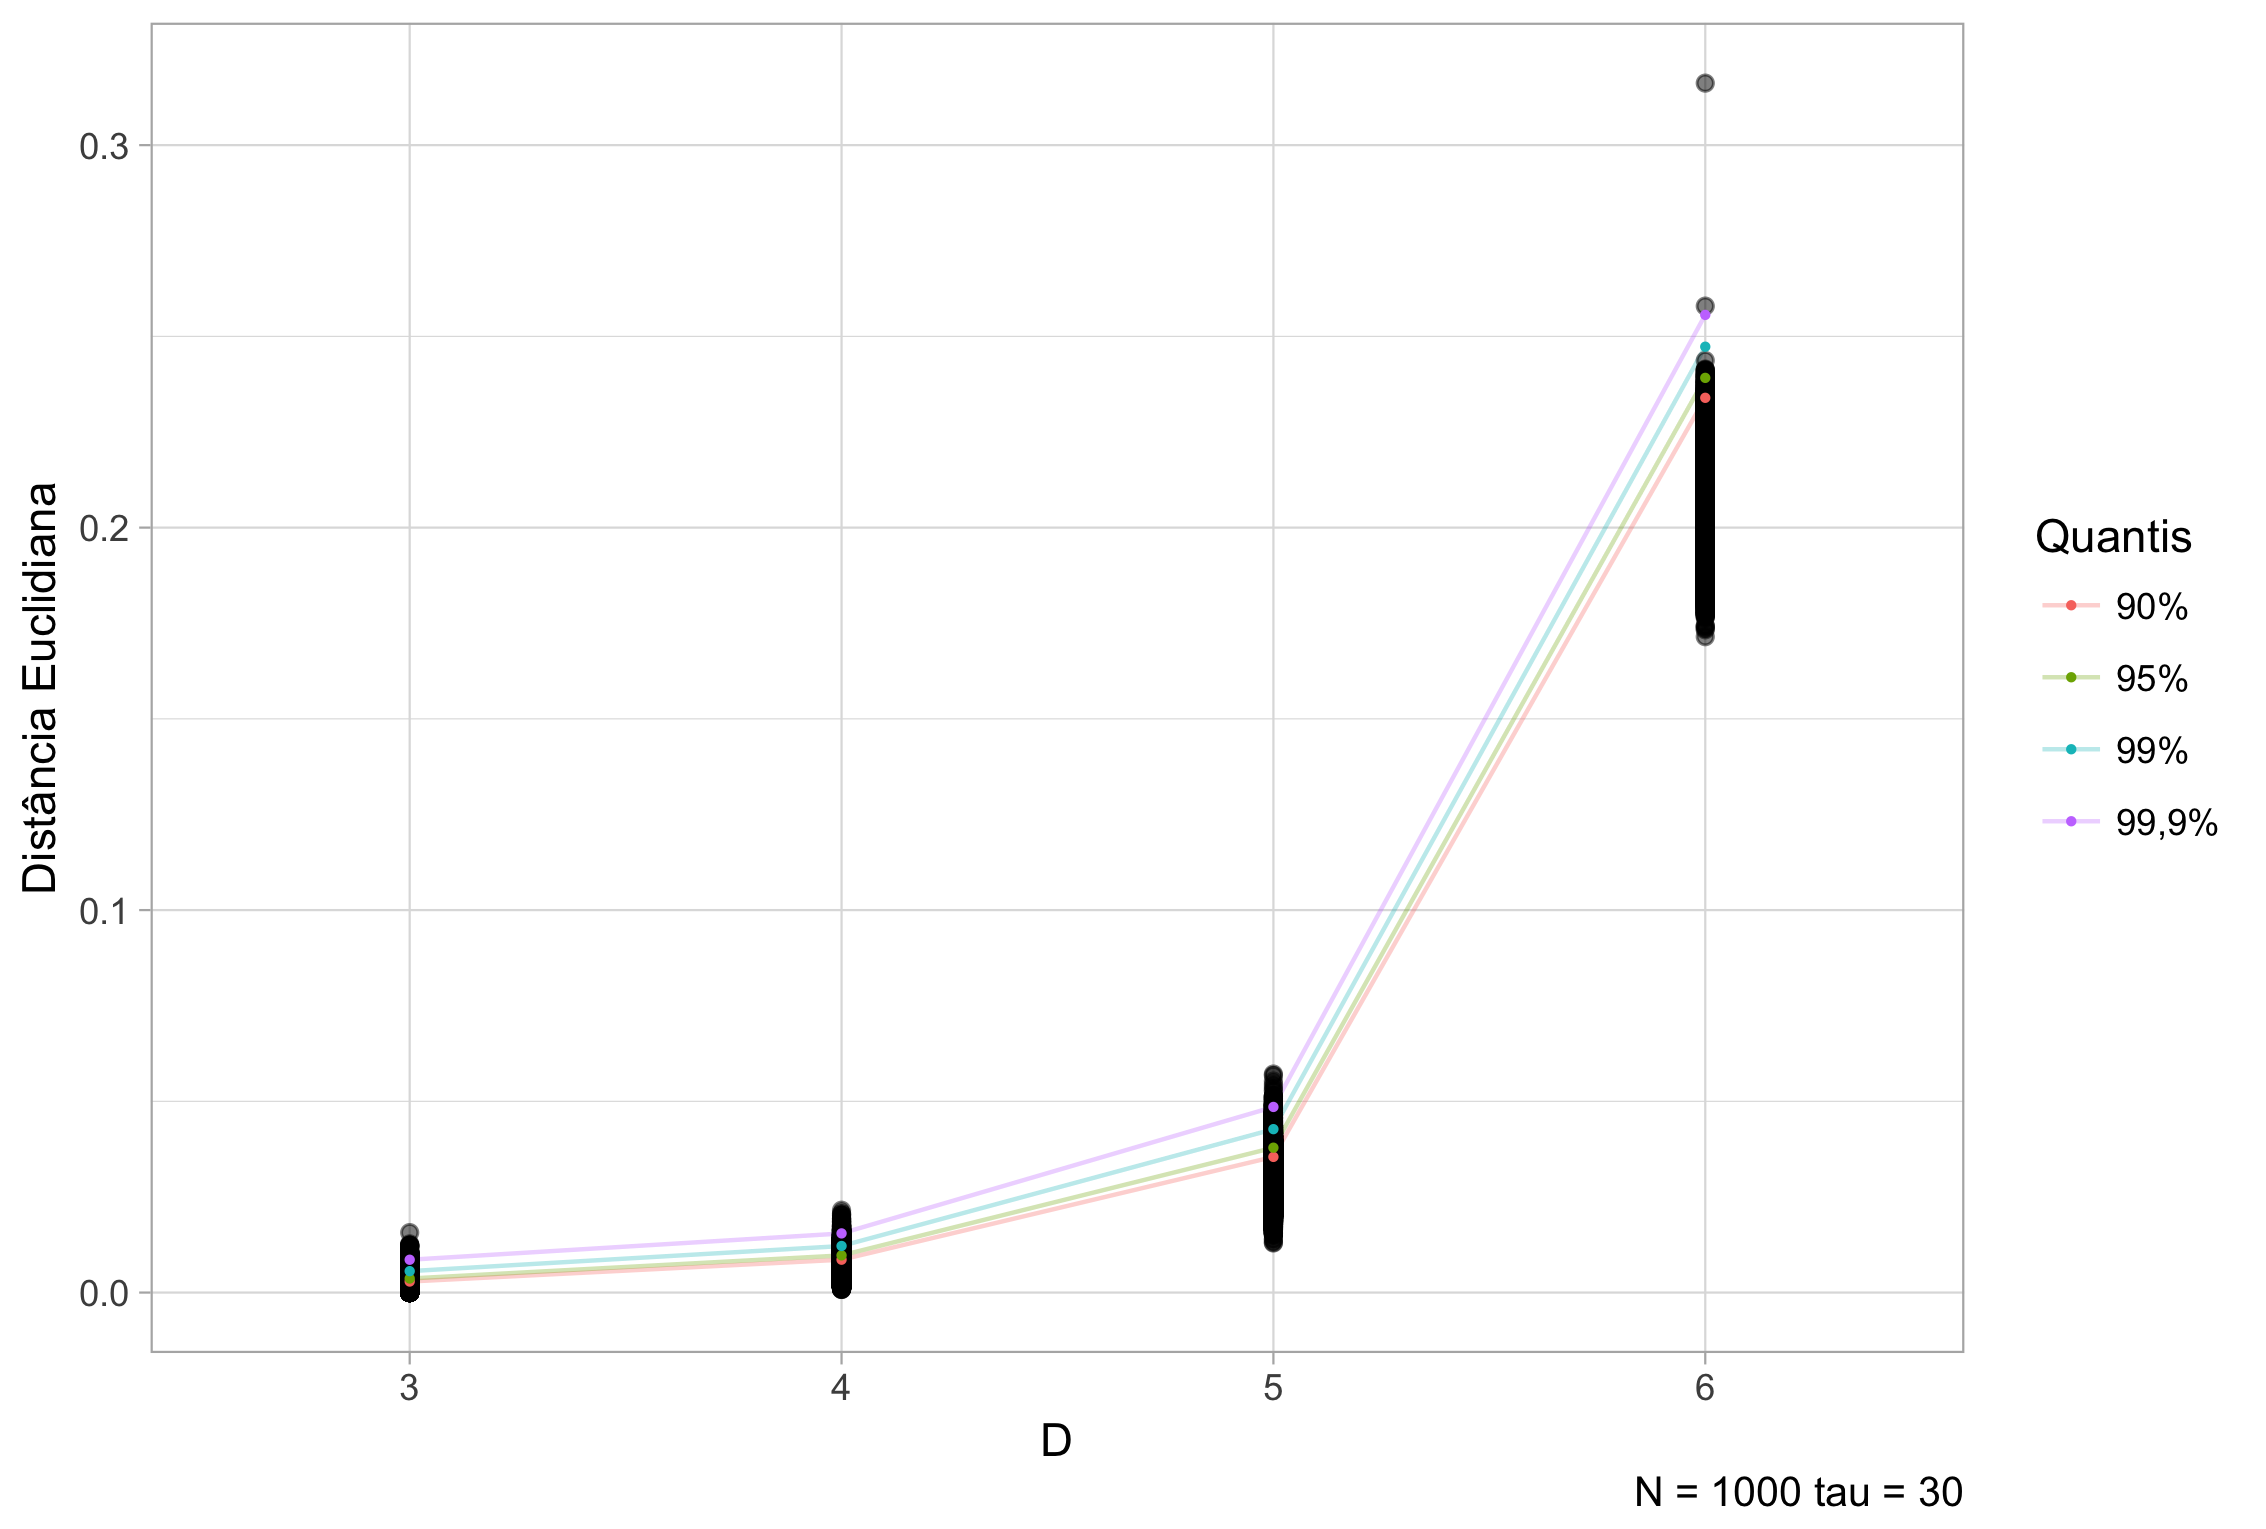
\includegraphics[width=1\linewidth]{Conf_Int_1k_T30_noMT}
	\caption{Intervalos de confiança para o caso $N=1.000$ e $\tau=30$.}\label{Fig:Conf_Int_1k_30}
\end{figure}

\begin{figure}
	\centering
	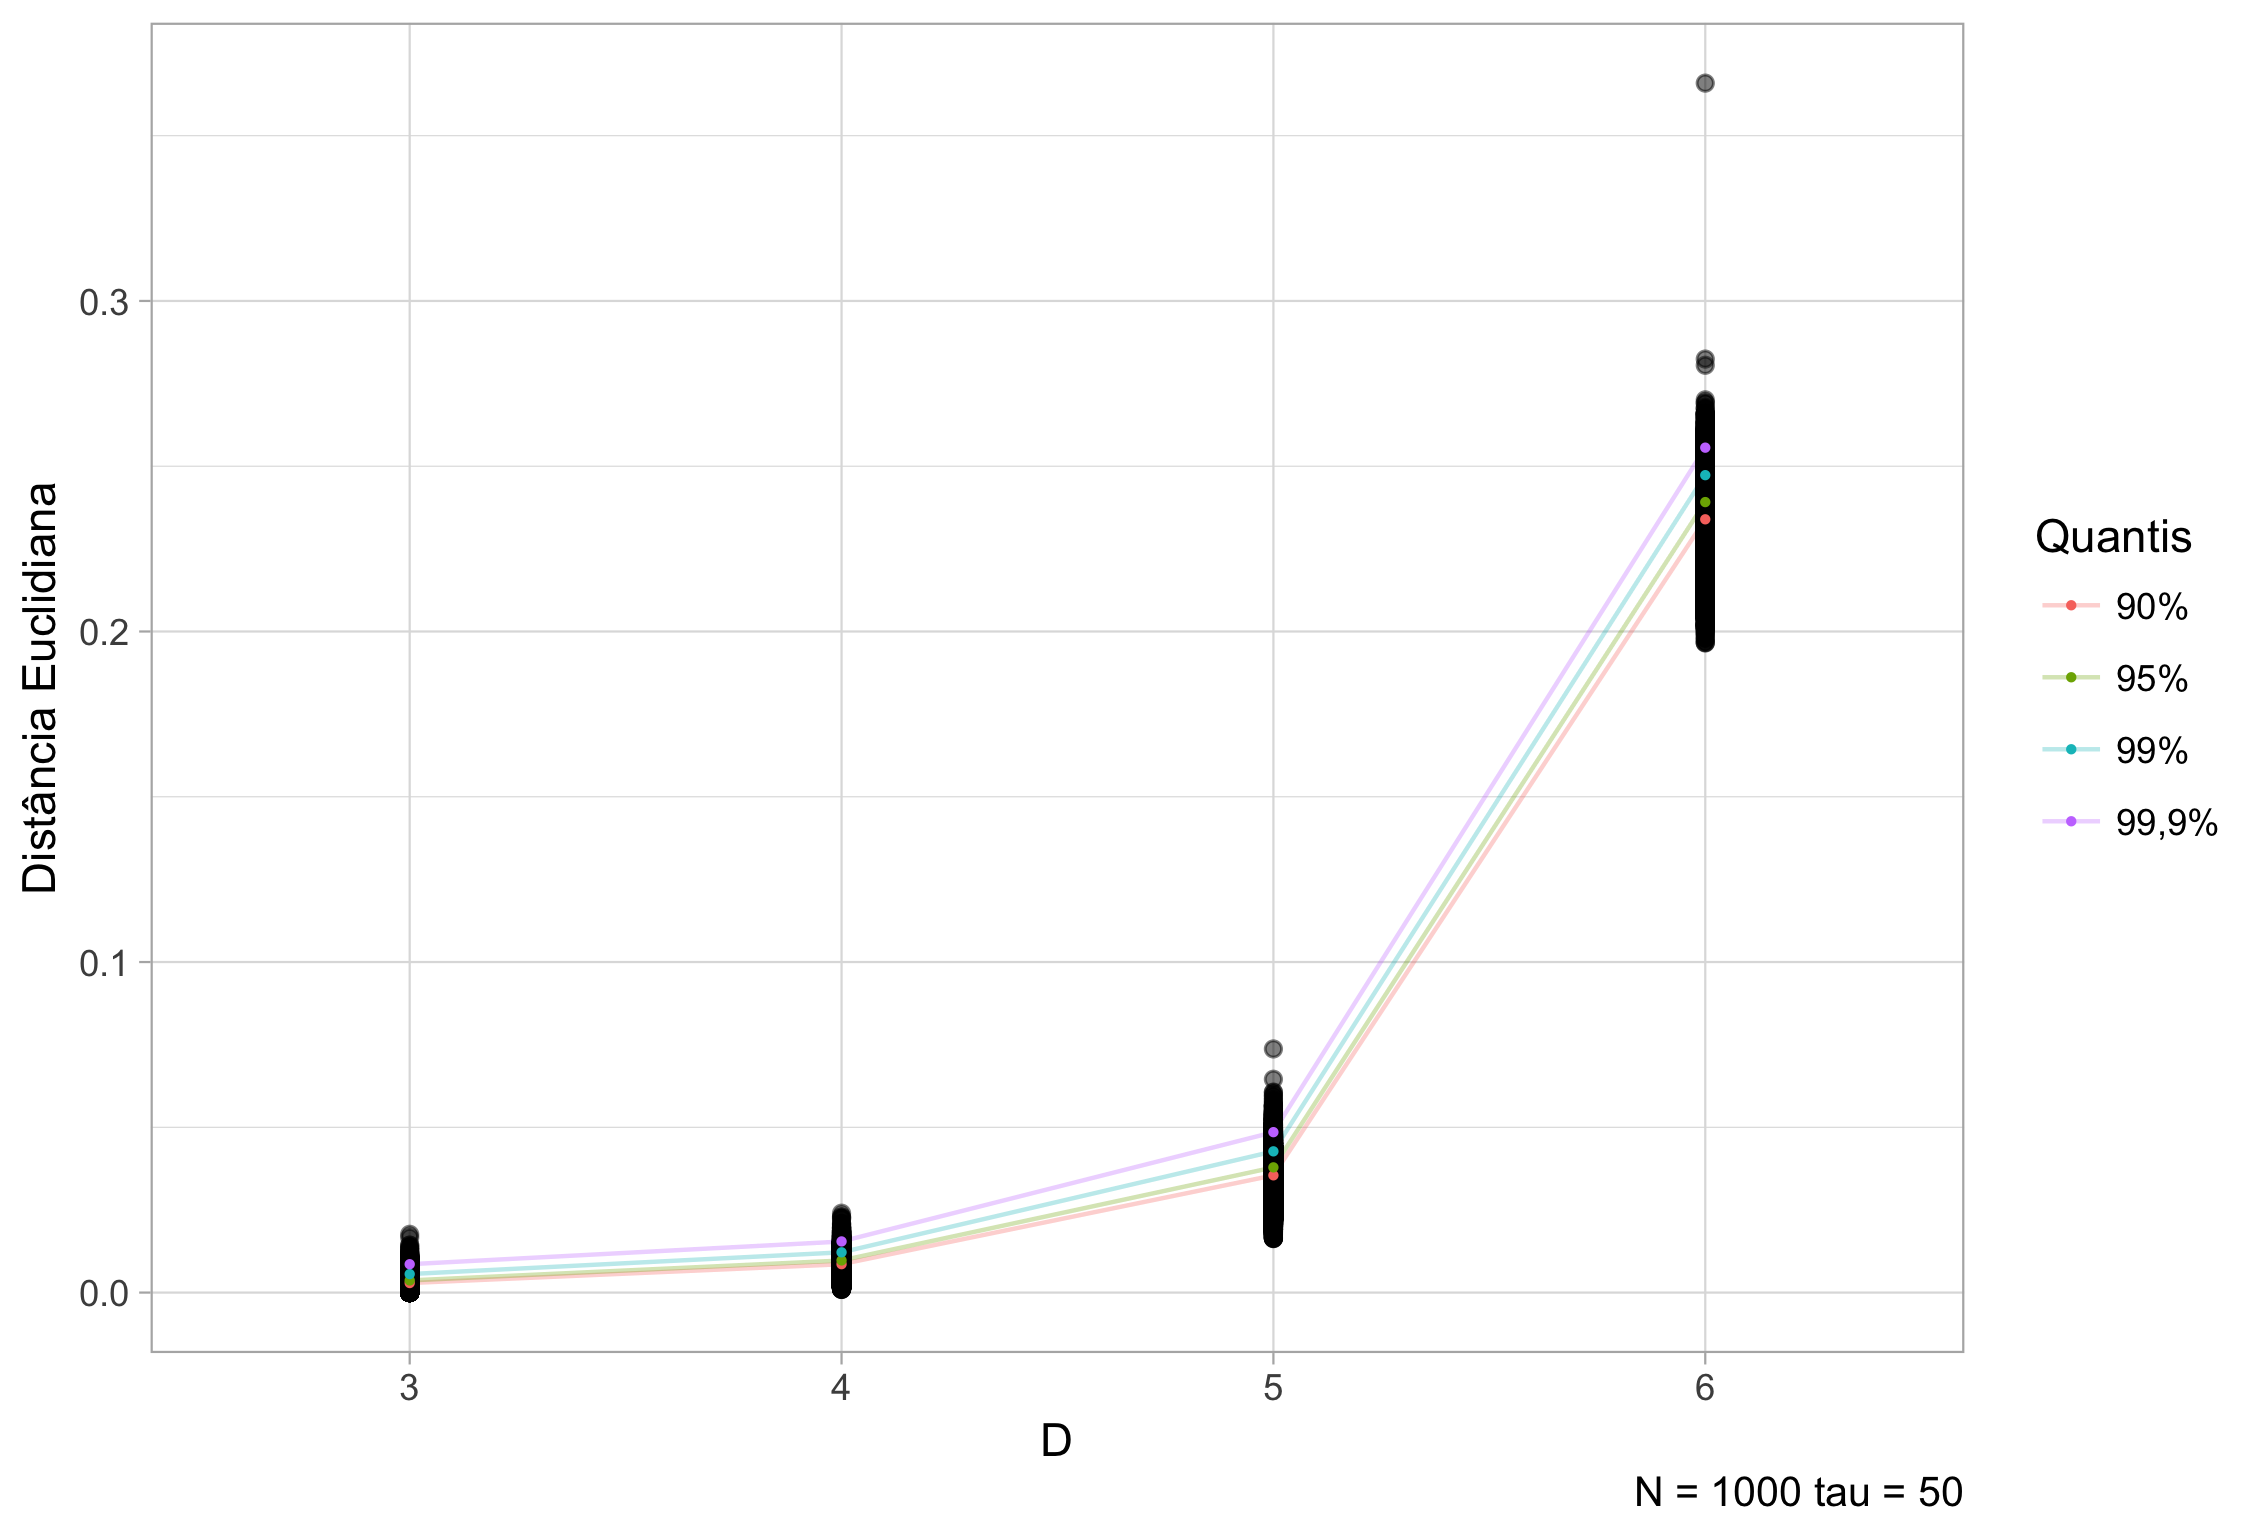
\includegraphics[width=1\linewidth]{Conf_Int_1k_T50_noMT}
	\caption{Intervalos de confiança para o caso $N=1.000$ e $\tau=50$.}\label{Fig:Conf_Int_1k_T50}
\end{figure}
%%

%% N=50.000
\begin{figure}
	\centering
	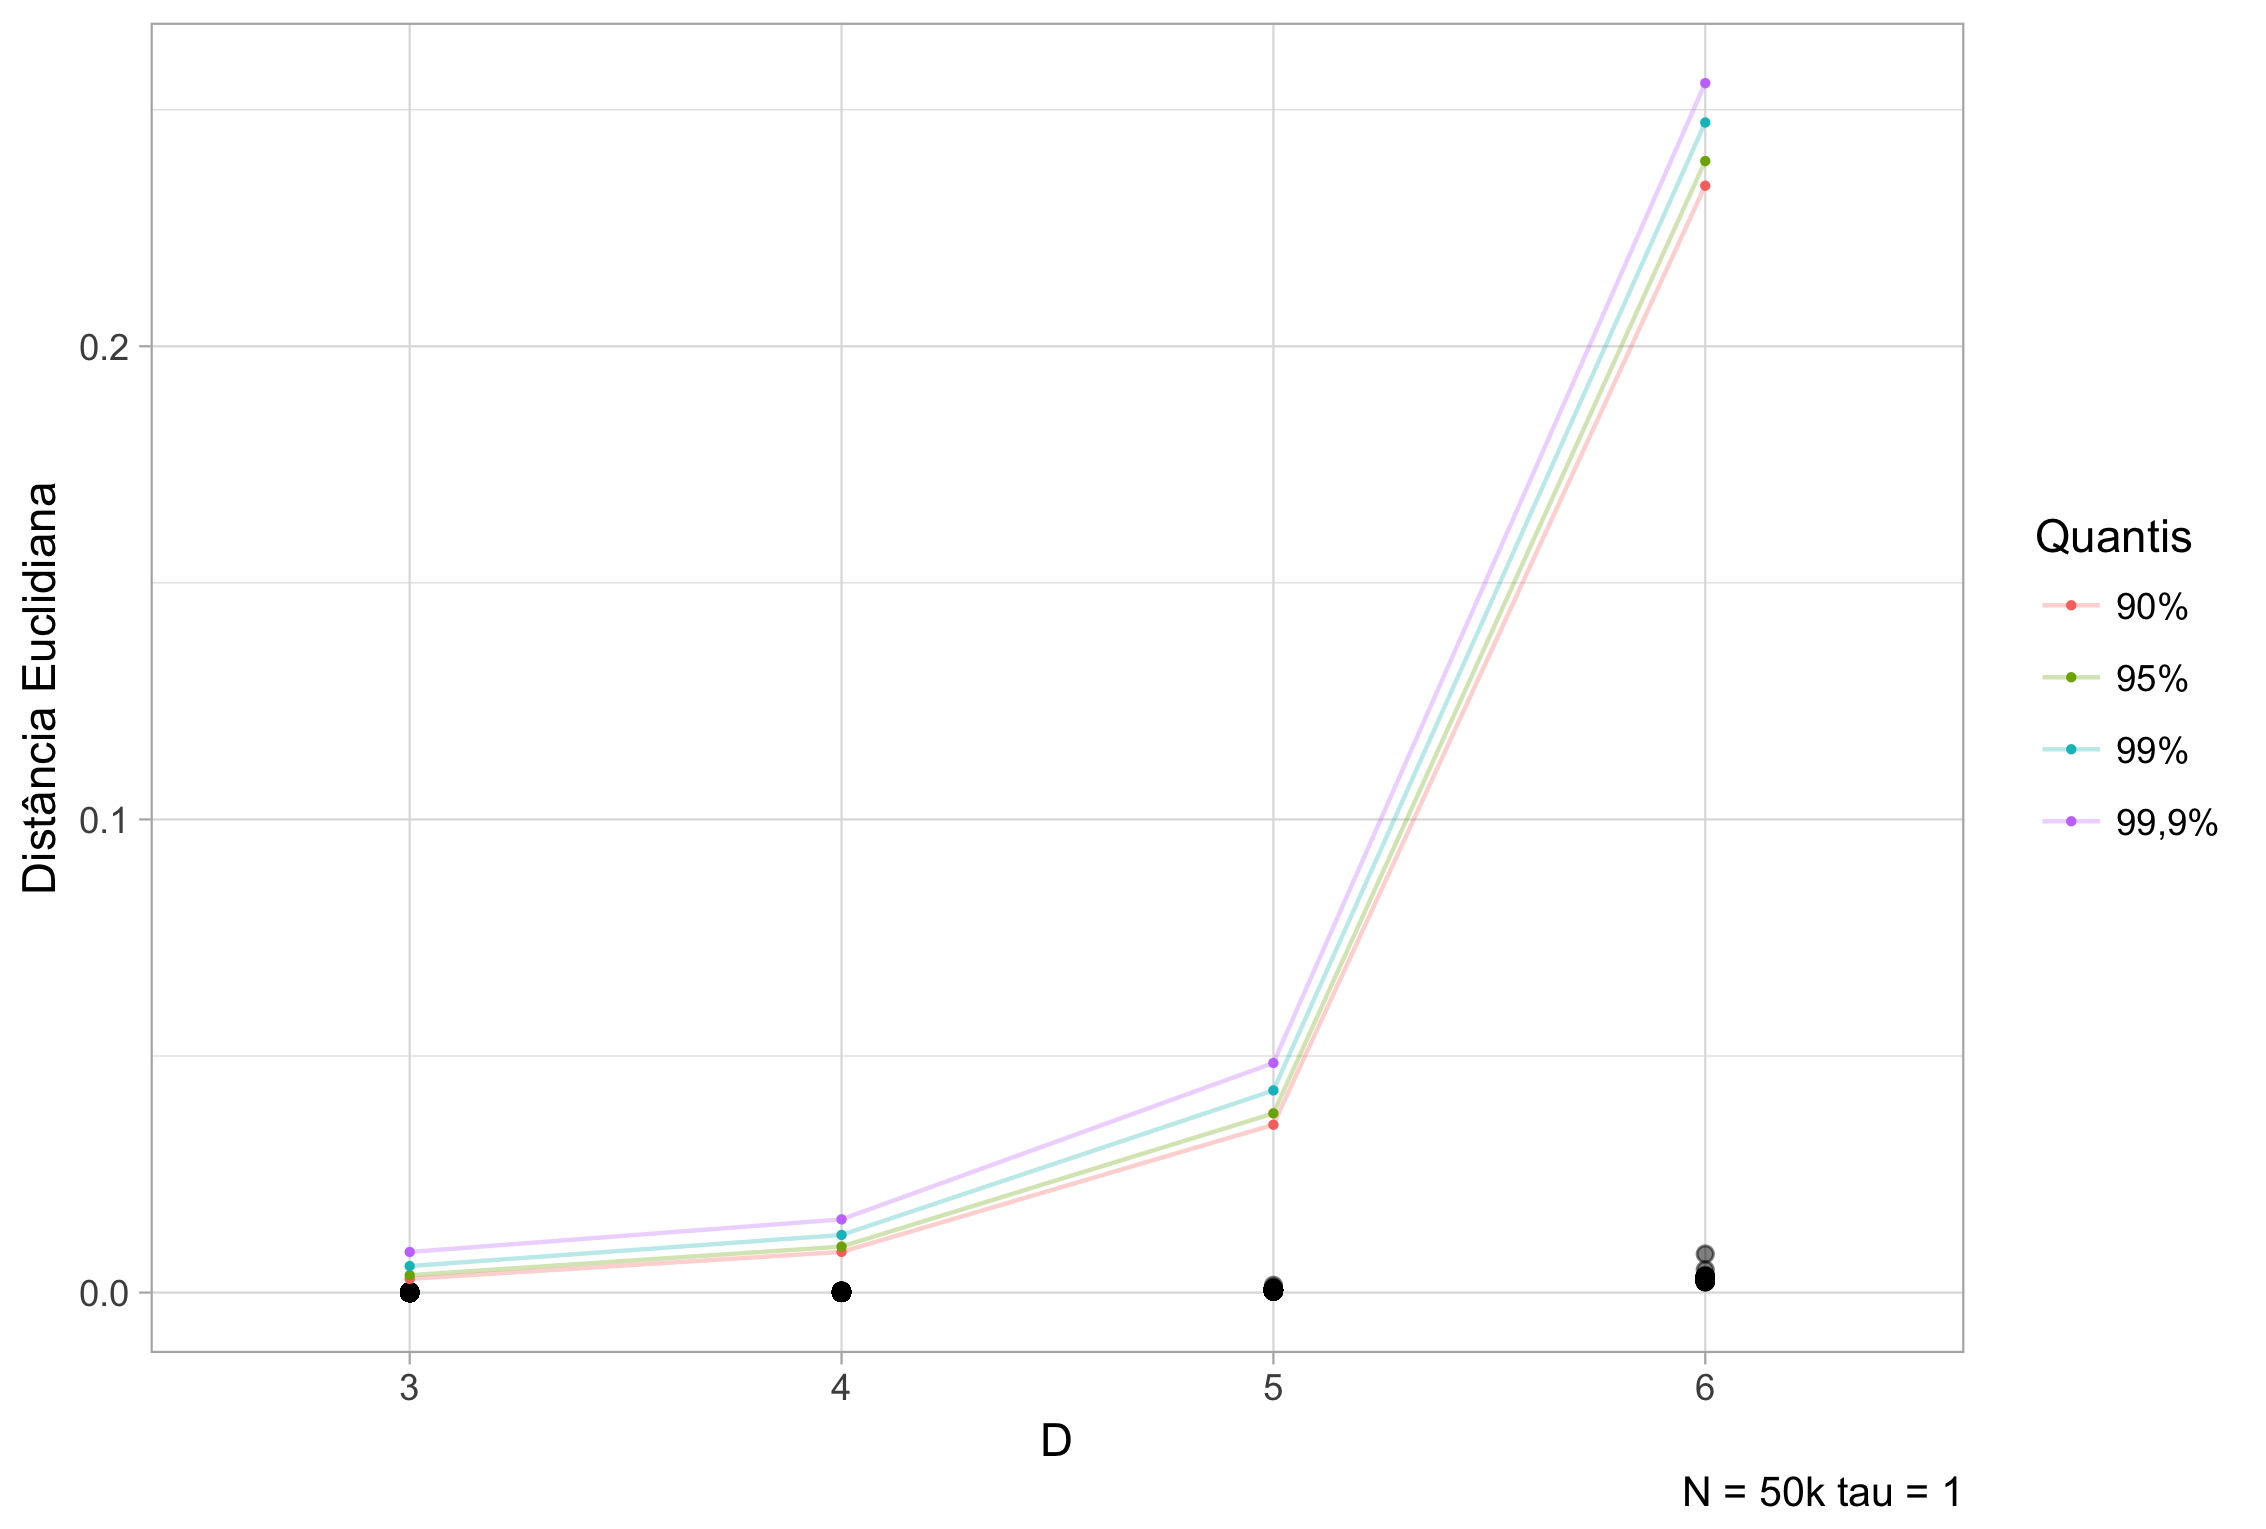
\includegraphics[width=1\linewidth]{Conf_Int_50k_T1_noMT}
	\caption{Intervalos de confiança para o caso $N=50.000$ e $\tau=1$.}\label{Fig:Conf_Int_50k_T1}
\end{figure}

\begin{figure}
	\centering
	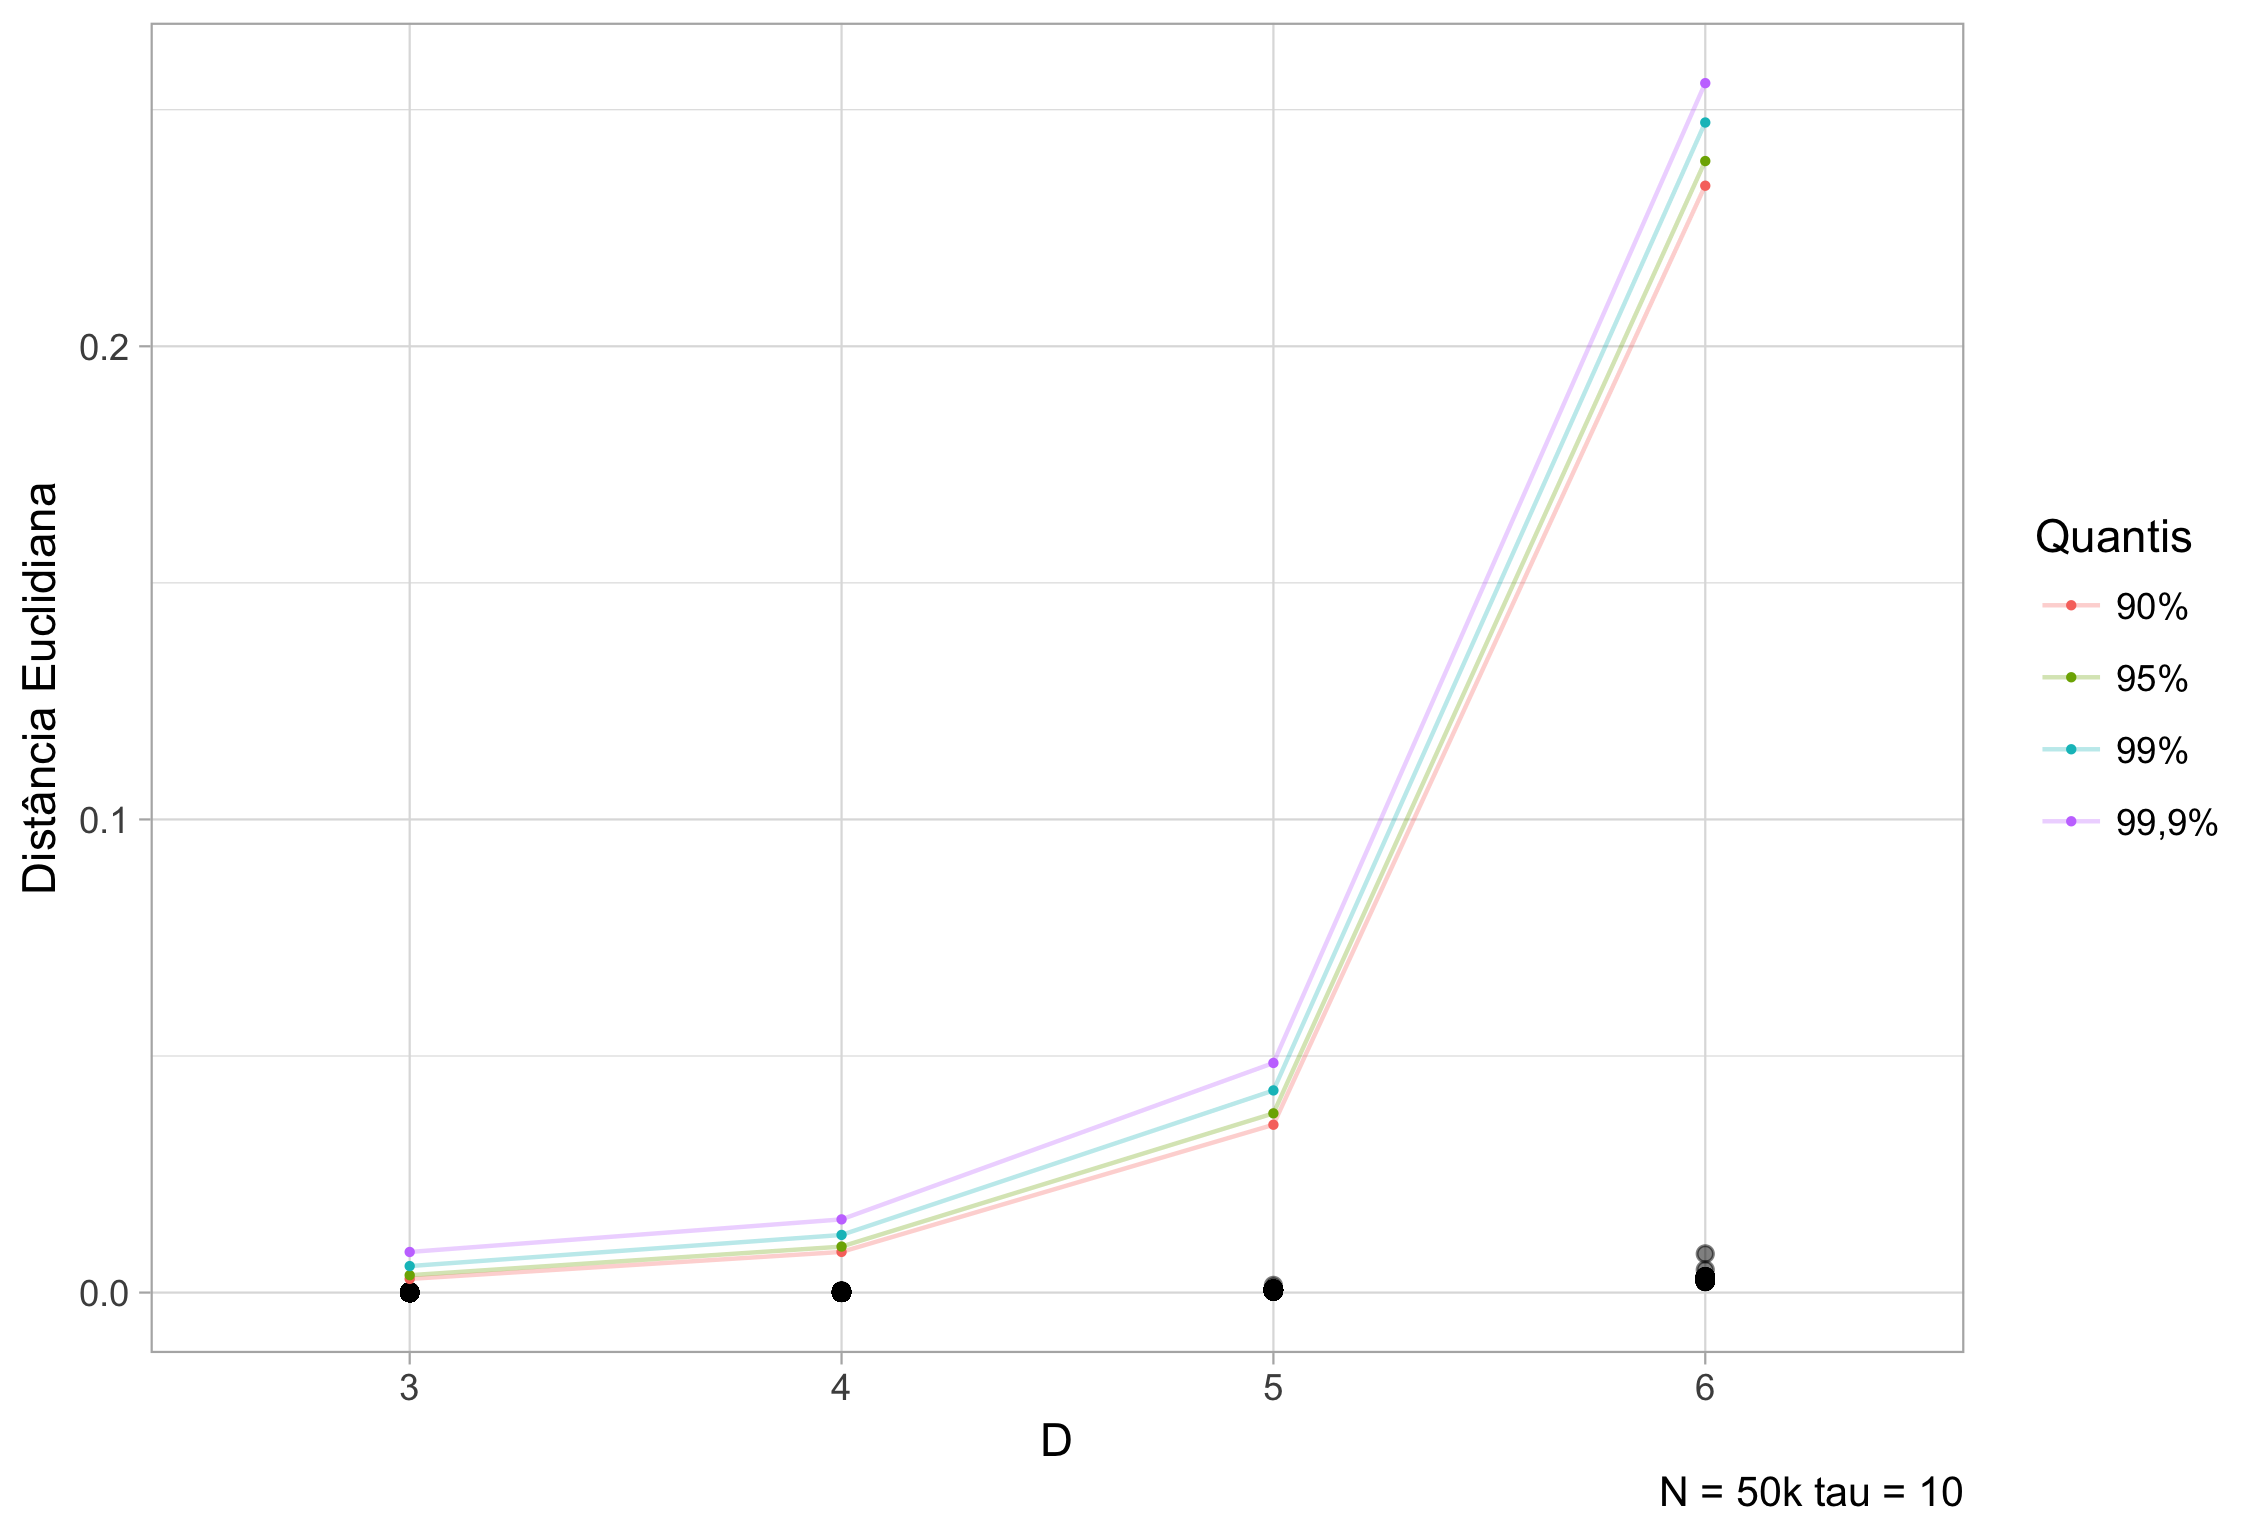
\includegraphics[width=1\linewidth]{Conf_Int_50k_T10_noMT}
	\caption{Intervalos de confiança para o caso $N=50.000$ e $\tau=10$.}\label{Fig:Conf_Int_50k_T10}
\end{figure}

\begin{figure}
	\centering
	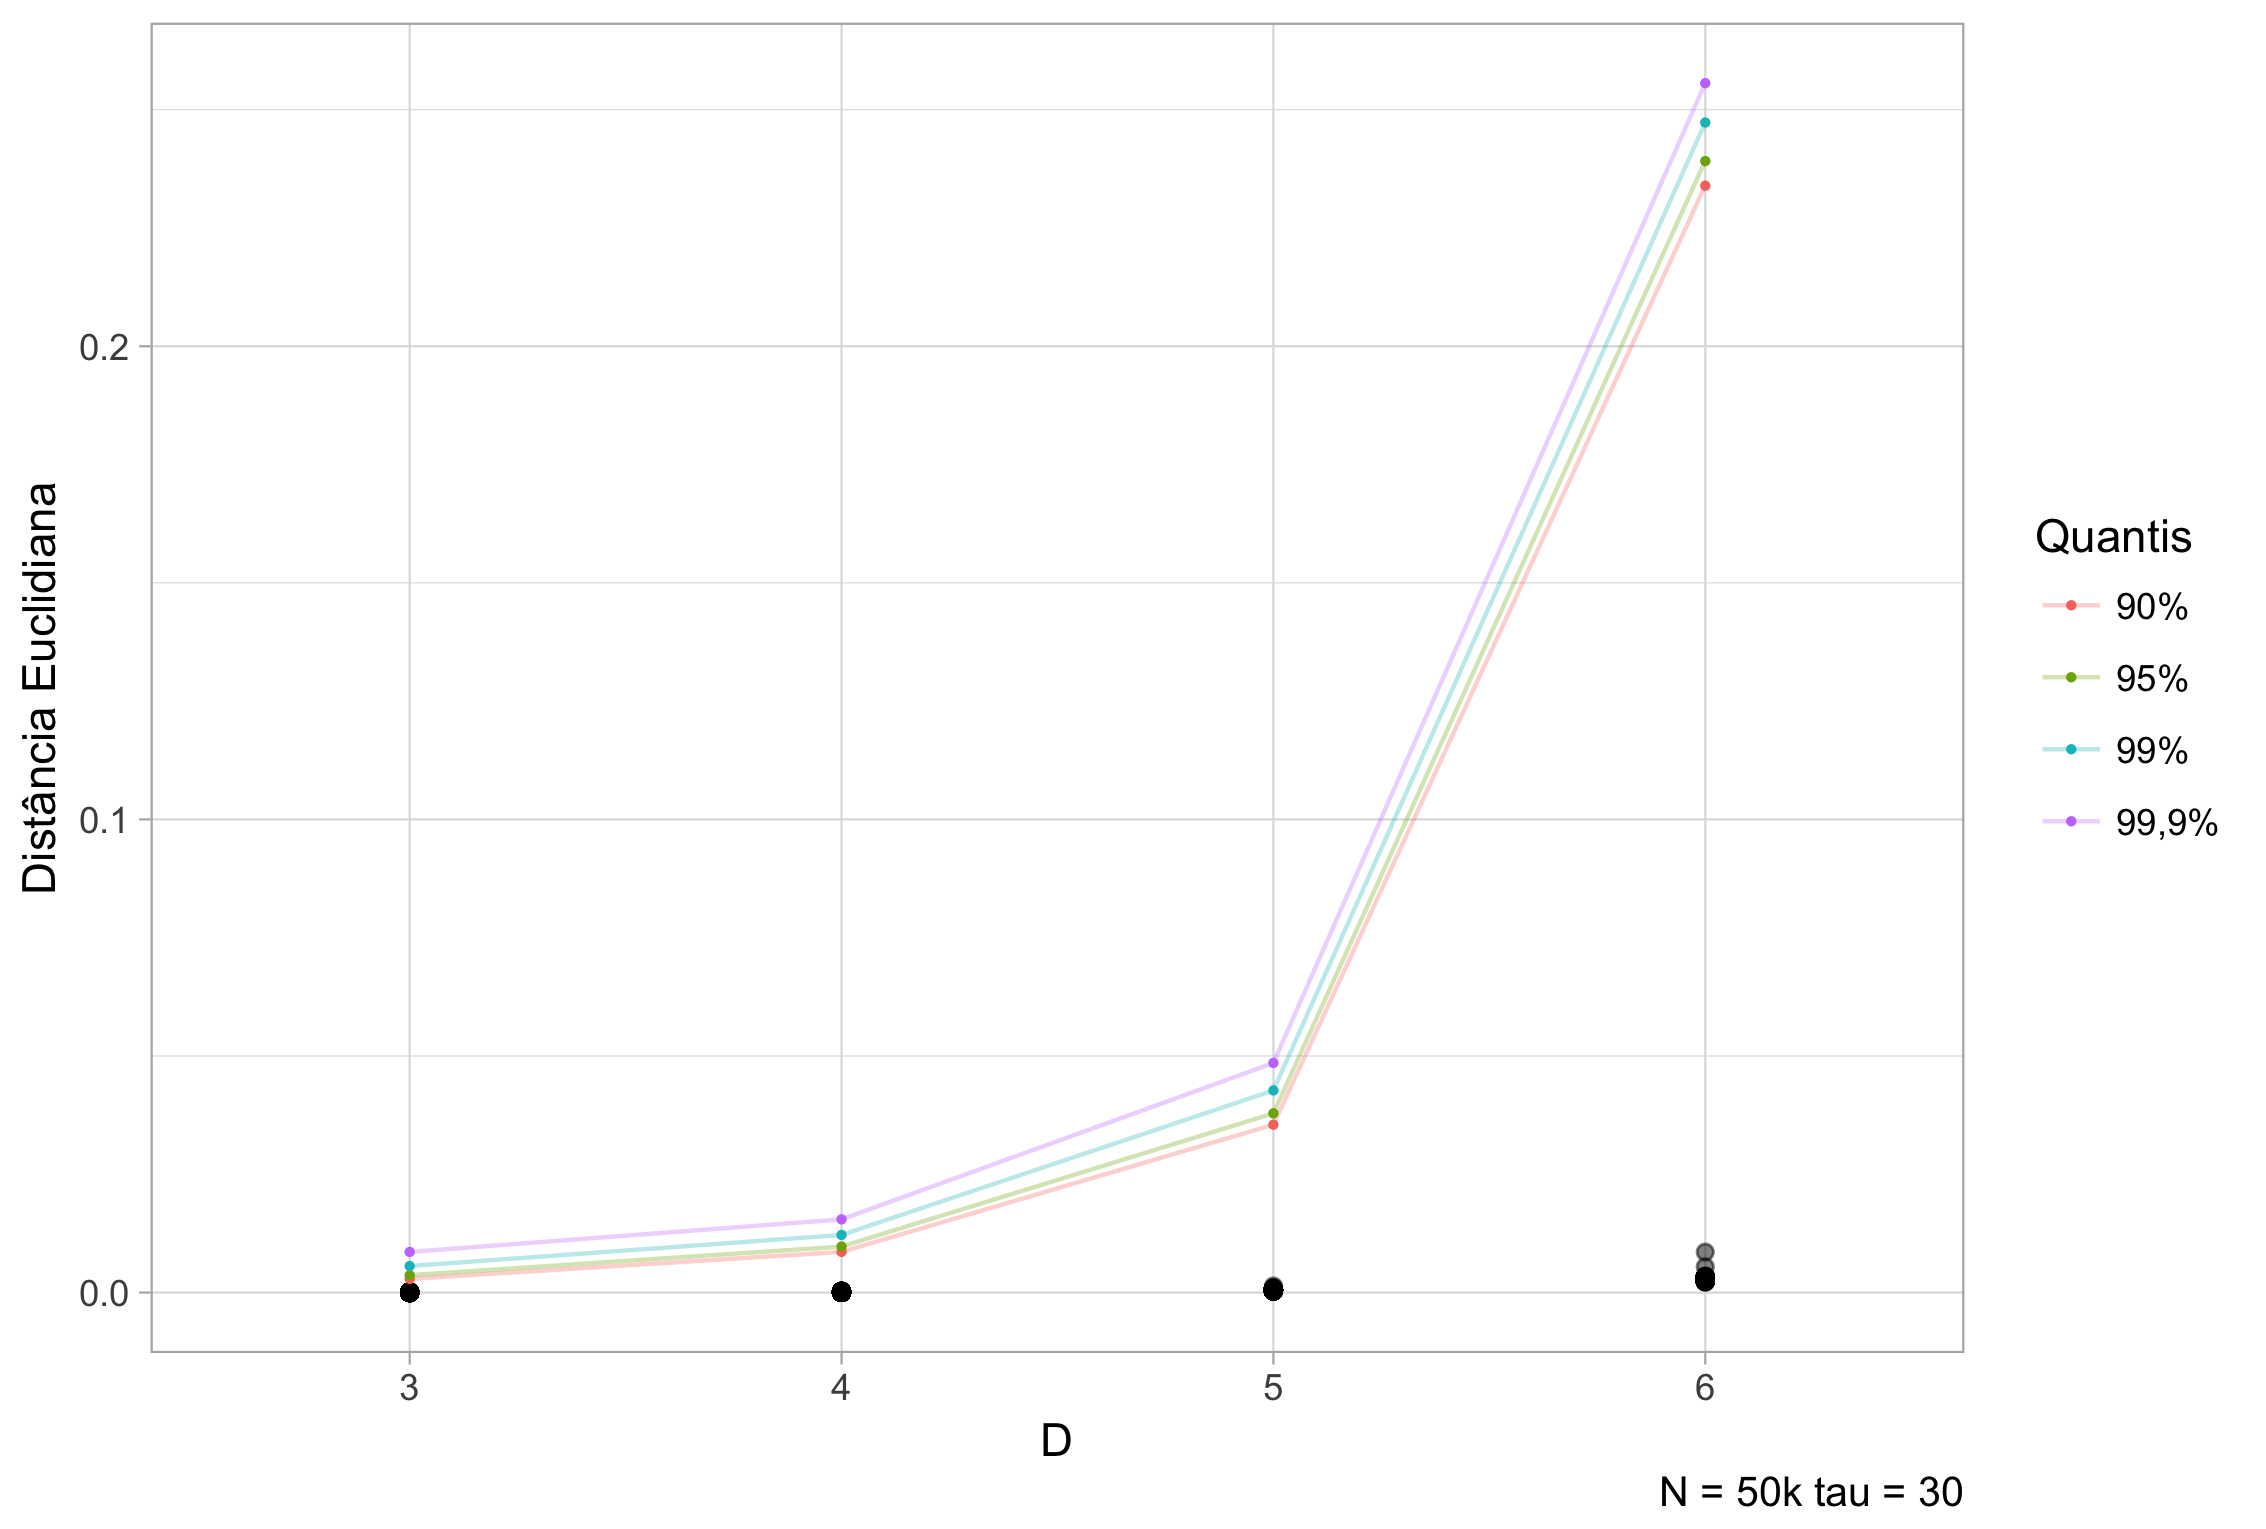
\includegraphics[width=1\linewidth]{Conf_Int_50k_T30_noMT}
	\caption{Intervalos de confiança para o caso $N=50.000$ e $\tau=30$.}\label{Fig:Conf_Int_50k_30}
\end{figure}

\begin{figure}
	\centering
	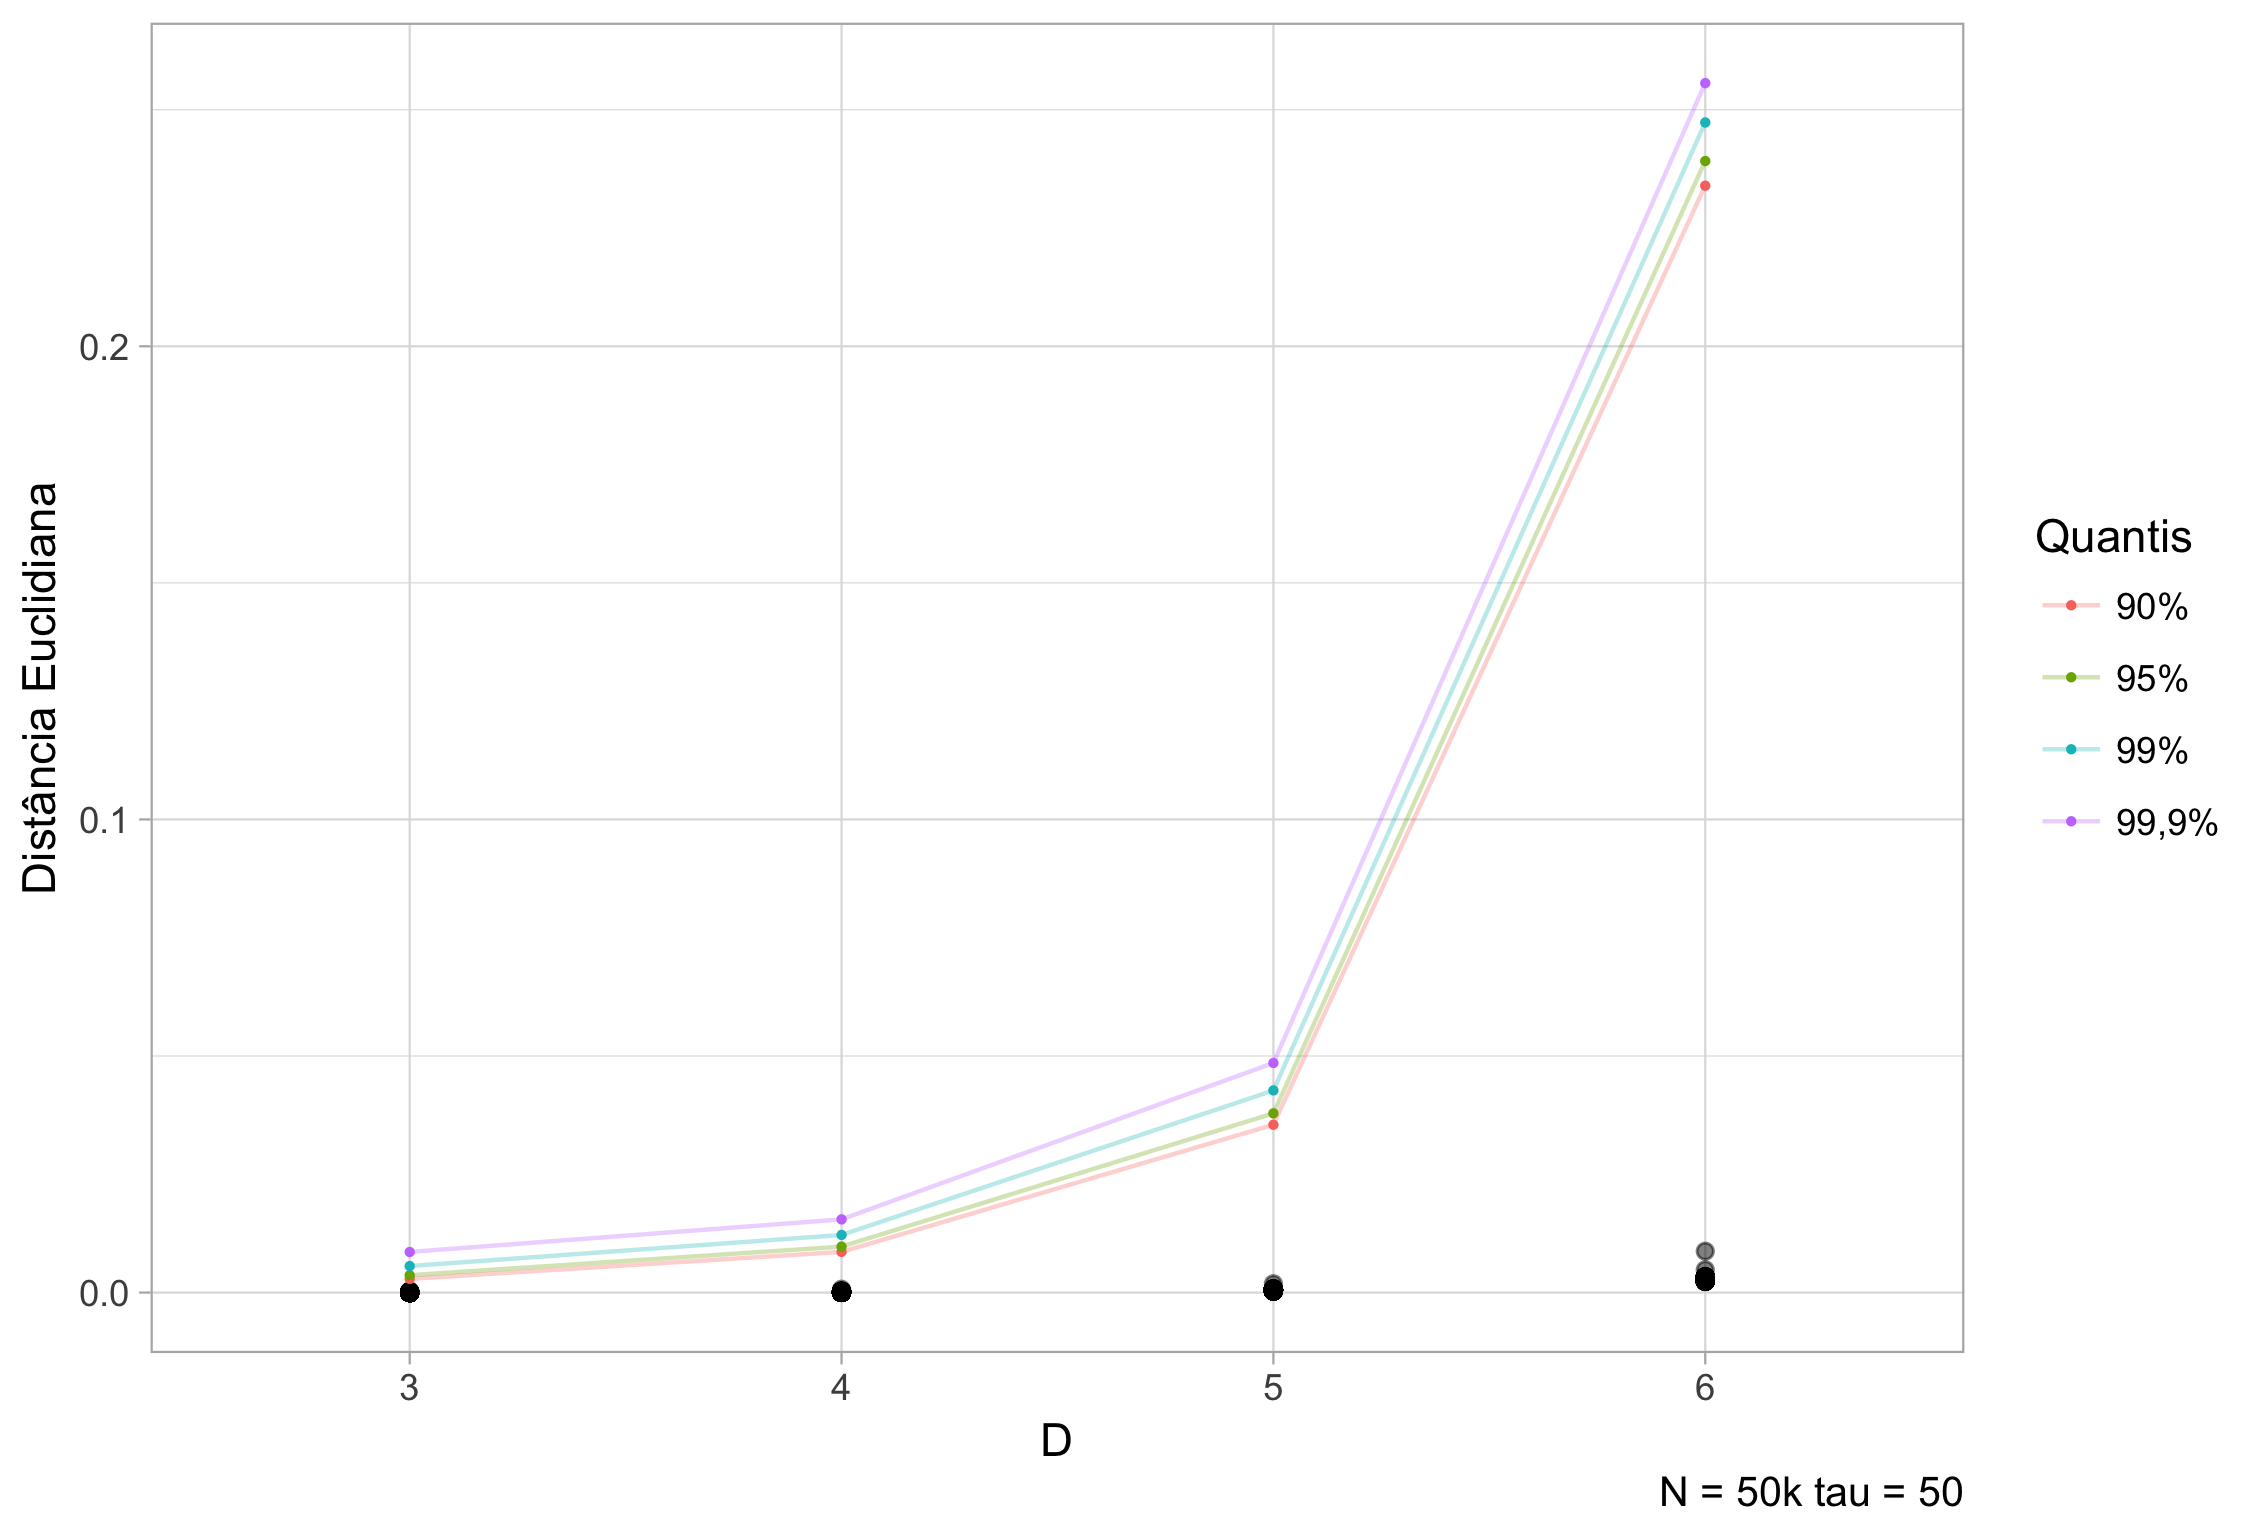
\includegraphics[width=1\linewidth]{Conf_Int_50k_T50_noMT}
	\caption{Intervalos de confiança para o caso $N=50.000$ e $\tau=50$.}\label{Fig:Conf_Int_50k_T50}
\end{figure}
%%


\begin{center}
	\fbox{
	\colorbox[RGB]{227, 227, 227}{
	\parbox[t]{.8\linewidth}
		{Neste capítulo tratamos os resultados esperados com a realização do trabalho enquanto que no próximo faremos a conclusão alcançada com o mesmo.}} }
\end{center}


\mychapter{Conclusão}{chp:conclusao}
\lhead{CONCLUSÃO}

Neste trabalho analisamos a possibilidade de a distância euclidiana de pontos no plano $(H\times C)$ de sequências ao ponto $(1,0)$, referência teórica de ruído branco, poderem ser usadas como uma estatística de teste para a hipótese de a sequência ser ruído branco.
Verificamos que essa possibilidade existe, e que essa estatística é capaz de identificar, com limitações, o mapa logístico (que já foi usado como gerador de números pseudoaleatórios), movimento browniano e ruído com autocorrelação.
Para este último, fizemos uma análise preliminar do poder do teste em função da intensidade da correlação.

Verificamos, também, que os geradores Mersenne-Twister e Randu são considerados ruído branco, mesmo sendo eles técnicas algorítmicas de geração de observações pseudoaleatórias.

A técnica permite discriminar observações de ruído browniano (não estacionário), do mapa logístico e, com limitações, de ruído estacionário obtido pela convolução de uma sequência de ruído branco com uma máscara.
Sendo a máscara parametrizada, fizemos uma análise preliminar do poder do teste.

Uma limitação deste trabalho é que apenas verificamos a qualidade do gerador em relação a um de estrutura ideal.
Com isso, limitamos a aplicabilidade do nosso trabalho à análise de séries que, potencialmente, são ocorrências de variáveis aleatórias independentes e identicamente distribuídas.

Há farta literatura que caracteriza diferentes tipos de estruturas como, por exemplo, processos estocásticos do tipo $f^{-k}$.
A nossa metodologia pode, em princípio, ser aplicada a quaisquer processos mas, para isso, é necessário o conhecimento da distribuição dos padrões ordinais do processo de referência.
No nosso caso, trata-se da lei uniforme sobre os padrões, que é característica de ruído branco.
Não conhecemos resultados que caracterizem de forma teórica as leis de outros processos.

Há, contudo, uma solução para esse problema: estimar a lei característica do padrão de interesse.
Isso pode ser feito através de estudos Monte Carlo, mas tal extensão foge ao objetivo deste trabalho.


\appendix

\chapter{Apêndice 1 - Agoritmos}\label{codigo}


\begin{lstlisting}[language=R, caption={Mersenne Twister}, label=code:MersenneTwister]
set.seed(1234567890, kind = "Mersenne-Twister")

MT1k <- runif(1000)
MT50k <- runif(50000)
\end{lstlisting}

\begin{lstlisting}[language=R, caption={Randu}, label={code:Randu}]
RANDU <- function() {
seed <<- ((1103515245 * seed) + 12345 ) %% (2^31)
}

Randu1k <- vector()
for(i in 1:1000) {

Randu1k[i] <- c(RANDU())
}
\end{lstlisting}


\begin{lstlisting}[language=R, caption={Não Estacionária}, label={code:NaoEstacionaria}]
NoEst1k <- diffinv(rnorm(1000))
NoEst1k <- abs(NoEst1k/max(NoEst1k))

NoEst50k <- diffinv(rnorm(50000))
NoEst50k <- abs(Randu50k/max(NoEst50k))
\end{lstlisting}


\begin{lstlisting}[language=R, caption={Estacionária}, label={code:Estacionaria}]
Est1k <- filter(rnorm(1000), filter=rep(1,3), circular=TRUE)

Est50k <- filter(rnorm(50000), filter=rep(1,3), circular=TRUE)
\end{lstlisting}


\begin{lstlisting}[language=R, caption={Mapa Logístico}, label={code:MapaLogistico}]
logisticmap <- function(N, x0) {

saida <- vector(mode="double", length=10000)
saida[1] <- x0

for(i in 2:10000)
saida[i] <- 4 * saida[i-1] * (1 - saida[i-1])

x0 <- saida[10000]
saida <- vector(mode="double", length=N)
saida[1] <- x0

for(i in 2:N)
saida[i] <- 4 * saida[i-1] * (1 - saida[i-1])

return(saida)
}

LogMap1k <- logisticmap(1000, .01)
LogMap50k <- logisticmap(50000, .01)

\end{lstlisting}


\begin{lstlisting}[language=R, caption={}, label={code:}]

\end{lstlisting}


% Apêndices e Anexos
\appendix
% % \mychapter{\textsc{Ambiente Reprodutível e Computacional}}{app:ambiente}
\chapter{\textsc{Ambiente Reprodutível e Computacional}}~\label{app:ambiente}
\lhead{\textsc{Ambiente Reprodutível e Computacional}}


\lettrine{O}{} \citet{ISI2012} 

%======================================================%
%============= REFERÊNCIAS BIBLIOGRÁFICAS =============%
%======================================================%
\begin{raggedright}
\renewcommand{\bibsection}{
\chapter*{\vspace{-3cm}\centering \Large \textsc{Referências Bibliográficas}}
\addcontentsline{toc}{chapter}{Referências Bibliográficas}
}
\lhead{\textsc{Referências Bibliográficas}}
\bibliography{references}
\newpage\lhead{\rightmark}
\end{raggedright}

%======================================================%

\chapter*{}
\vfill
\singlespacing
\thispagestyle{empty}
\begin{center}

\includegraphics[width=.3\textwidth]{./capitulos/figs/knot}

\vspace{.5cm}

Este trabalho foi redigido em {\large \LaTeX}\ utilizando uma modificação do estilo \textsf{IC-UFAL}.
As referências bibliográficas foram preparadas no \textsf{JabRef} e administradas pelo {\large\BibTeX}\ com o estilo \textsf{LaCCAN}.
O texto utiliza fonte \NomeFonte\ e os elementos matemáticos a família tipográfica \NomeFonteMat, ambas em corpo de 12 pontos.
% A numeração dos capítulos segue com a família tipográfica \NomeFonteCap.\\ 
\vspace{.5cm}
%
\includegraphics[width=.5\textwidth]{./capitulos/figs/celtic_knot_cross_stitch}
\end{center}

\end{document}
